%% AIAA Journal submission. Uses the AIAA class `new-aiaa` (Overleaf), journal format:
%% single-column, double-spaced, 10pt Times. Requires new-aiaa.cls + new-aiaa.bst (this directory)
%% and the newtx fonts. Build: pdflatex main; bibtex main; pdflatex main; pdflatex main.
\documentclass[journal]{new-aiaa}

\usepackage{graphicx}
\usepackage{float}
\usepackage[section]{placeins}  % keep floats within their section (no drift into later sections)
\usepackage{amsmath}
\let\Bbbk\relax  % this TeX Live predefines \Bbbk; free the name so amssymb can redefine it
\usepackage{amssymb}
\usepackage{booktabs}
\usepackage{CJKutf8}  % Daodejing epigraphs + inline terms (user-tree install: tlmgr --usermode, TL2021 historic repo)

\renewcommand{\topfraction}{0.9}
\renewcommand{\bottomfraction}{0.8}
\renewcommand{\textfraction}{0.07}
\renewcommand{\floatpagefraction}{0.8}

\graphicspath{{figs/}}

\title{A One-Equation Transition Model: Autogenous Inception from the
Spalart--Allmaras Working Variable}

\author[1,2]{Qiqi Wang\footnote{Founding Technologist, Flexcompute, Inc.;
Associate Professor, Department of Aeronautics and Astronautics, Massachusetts
Institute of Technology. AIAA Associate Fellow.}}
\affil[1]{Flexcompute, Inc.}
\affil[2]{Department of Aeronautics and Astronautics, Massachusetts Institute of Technology}

\begin{document}
\maketitle

\begin{abstract}
We present a one-equation Reynolds-averaged Navier--Stokes (RANS) transition
model in which the Spalart--Allmaras (SA) working variable $\tilde\nu$ serves as
its own transition indicator. We repurpose its sub-$O(1)$ range---inert in the
baseline model---as a Tollmien--Schlichting amplification factor: a blended
production term---with the destruction tied to it and the molecular diffusion
coefficient reduced in the $\tilde\nu$ equation only---drives the SA transport
equation, unchanged in structure,
through laminar instability growth and turbulent eddy-viscosity production,
handing over near $\chi\!=\!\tilde\nu/\nu\!\sim\!1$. No auxiliary field is
introduced. The amplification rate depends only on the local mean
flow---a vorticity Reynolds number and two profile-shape indicators, a
vorticity fraction and an accumulated-inflection (Rayleigh) coordinate---with no
pressure-gradient parameter anywhere, and
is anchored to canonical stability limits: the free-shear growth
eigenvalue, the linear-stability onset of the Falkner--Skan family, and
the Blasius $e^N$ envelope; the freestream seed is set by Mack's
receptivity correlation. The
model is tested on three cases spanning zero, favorable, and adverse
pressure gradients---a flat plate, the NLF(1)-0416 airfoil at
$Re\!=\!4\!\times\!10^6$, and the Eppler 387 at
$Re\!=\!6\!\times\!10^4$--$4.6\!\times\!10^5$---across wide incidence ranges,
on structured and unstructured meshes at three refinement levels, with
the same constants throughout. The Eppler Reynolds sweep locates the
model's bubble-bursting boundary one Reynolds step above the measured
one and traces the displacement to the deliberately unmodeled
transition zone. The model is also deployed in three
dimensions on the wing of the Daedalus human-powered aircraft.
\end{abstract}

\begin{center}
  \begin{minipage}{0.6\textwidth}\centering
  \begin{CJK}{UTF8}{bsmi}埏埴以為器，當其無，有器之用。\end{CJK}\\[3pt]
  \emph{Clay is shaped into a vessel:\\
  it is the emptiness within that makes it useful.}\\[3pt]
  ---\emph{Daodejing}, ch.~11
  \end{minipage}
\end{center}

\section*{Nomenclature}
\begin{tabbing}
  $N,\;N_\mathrm{crit},\;Re_\Omega^{\mathrm{c}}$\quad\quad \= \kill
  $\tilde\nu$ \> SA working variable \\
  $\tilde S$ \> SA modified vorticity \\
  $\nu,\;\nu_t$ \> kinematic (laminar) and eddy viscosity ($\nu_t=\tilde\nu[(1-b)f_{v1}+b]$, Eq.~\eqref{eq:fv1bypass}) \\
  $c_{v1},\;f_{v1}$ \> SA near-wall constant and function \\
  $P,\;D$ \> production and destruction of $\tilde\nu$ \\
  $P_\mathrm{SA},\;P_\mathrm{AI}$ \> turbulent (SA) and laminar-amplification production terms \\
  $c_{\nu,\mathrm{ai}}$ \> laminar-viscosity scale in the SA diffusion term only ($1/6$) \\
  $\hat\nu$ \> disturbance field of the parabolized march, Eq.~\eqref{eq:transport} \\
  $\chi,\;\chi_\infty$ \> $\tilde\nu/\nu$ and its freestream value \\
  $d$ \> distance to the nearest wall \\
  $\omega$ \> vorticity magnitude \\
  $Re_\Omega$ \> vorticity Reynolds number, $d^2\omega/\nu$ \\
  $X,\;Y,\;Z$ \> velocity, vorticity (shear), and curvature indicators, Eq.~\eqref{eq:indicators} \\
  $\hat\Omega,\;\lambda$ \> vorticity fraction $Y/\sqrt{X^2+Y^2}=\sin\lambda$ and longitude, Eq.~\eqref{eq:shat} \\
  $I,\;\hat I$ \> accumulated inflection $I=d\,u'-u-\tfrac12 d^2u''$ and its normalized (sphere) coordinate $\hat I=Y-X-Z$, Eqs.~\eqref{eq:parabola} and~\eqref{eq:g_integral} \\
  $\hat\Omega \hat I$ \> amplifying (rate) coordinate: the even product of the vorticity fraction and the accumulated-inflection coordinate, Eq.~\eqref{eq:rate} \\
  $\hat{\mathbf{n}}$ \> unit wall-normal direction (gradient of $d$) \\
  $a,\;a_{\max}$ \> laminar amplification rate and its free-shear ceiling ($0.19$) \\
  $Re_\Omega^{\mathrm{c}}(\hat\Omega \hat I)$ \> vorticity-Reynolds onset threshold, Eq.~\eqref{eq:reomc} \\
  $C,\;A,\;B,\;k$ \> onset-threshold shape constants and scale, Eq.~\eqref{eq:reomc} \\
  $Re_{\theta 0}(H)$ \> Drela--Giles critical (first-instability) momentum-thickness Reynolds number \\
  $w$ \> onset ramp width scale, Eq.~\eqref{eq:onset} \\
  $\sigma_P,\sigma_D;\;\tau$ \> production and destruction handover weights and the production width, Eq.~\eqref{eq:blend} \\
  $N,\;N_\mathrm{crit}$ \> amplification factor and its critical value ($e^N$ method) \\
  $Tu$ \> freestream turbulence intensity \\
  $p,\;\rho$ \> static pressure and density \\
  $|u|$ \> velocity magnitude relative to the nearest-wall point \\
  $\mathbf d,\;\boldsymbol\omega$ \> wall-distance vector $d\,\nabla d$ and vorticity vector \\
  $\boldsymbol\ell$ \> curvature vector $\tfrac12\langle\mathbf d,\mathbf d\rangle\,\nabla^2\mathbf u$, Eq.~\eqref{eq:gram} \\
  $\langle\cdot,\cdot\rangle$ \> Euclidean inner product of vectors \\
  $b;\;q,\;s,\;G$ \> f$_{v1}$-bypass blend weight and its gate inputs, Eqs.~\eqref{eq:fv1q}--\eqref{eq:fv1bypass} \\
  $H$ \> boundary-layer shape factor \\
  $\alpha$ \> angle of attack \\
  $c,\;x/c$ \> airfoil chord and chordwise coordinate \\
  $x_\mathrm{tr},\;x_R$ \> transition-onset and turbulent-reattachment locations \\
  $Re,\;M$ \> chord Reynolds number and Mach number \\
  $Re_x,\;Re_\theta$ \> streamwise and momentum-thickness Reynolds numbers \\
  $C_f,\;C_d,\;C_l$ \> skin-friction, drag, and lift coefficients \\
\end{tabbing}

\section{Introduction}

Laminar flow over a lifting surface offers one of the largest available
viscous-drag reductions, and predicting where it ends is a first-order requirement
for natural-laminar-flow design. This is not only a transport-aircraft concern:
at the low-to-moderate chord Reynolds numbers of general-aviation and sport
aircraft and of small---increasingly electric---rotors and drones, the laminar run
is a large fraction of the chord, and its extent sets efficiency, range and
endurance, and acoustic signature.
In a low-disturbance environment the laminar boundary layer first becomes
unstable to gentle two-dimensional Tollmien--Schlichting (TS) waves
\cite{mack_1977,schmid_henningson_2001}: as the layer thickens, the envelope of the
strongest TS mode grows quasi-exponentially over a long streamwise stretch until,
at an amplitude of a few percent of the mean, three-dimensional secondary
instabilities trigger localized turbulent spots that spread and merge into a fully
turbulent layer \cite{schubauer_klebanoff_1956,schmid_henningson_2001}. The slow
TS-envelope stage can occupy most of the streamwise distance and set
where transition is observed, so it is the stage a transition model must reproduce.
The classical tool is the $e^N$ method \cite{smith_gamberoni_1956, vaningen_2008}:
linear stability theory is integrated along the boundary layer to accumulate an
amplification factor $N$, and transition is declared where $N$ reaches an empirical
threshold $N_\mathrm{crit}$ set by the disturbance environment \cite{mack_1977}.
Drela and Giles reduced the stability integration to an approximate envelope
correlation, making $e^N$ practical inside an integral-boundary-layer method
\cite{drela_giles_1987, drela_xfoil_1989}.

The $e^N$ method is non-local: it presumes a boundary layer that can be marched and
integrated, which is foreign to a general unstructured RANS solver. The community
has therefore recast transition as locally computable transport equations,
along three lines. \emph{Amplification factor transport} carries $N$ itself: Coder
and Maughmer's AFT model transports an amplification factor whose source reproduces
the $e^N$ envelope and couples it to SA through the $f_{t2}$ term, the variant
catalogued as SA-AFT2017b on the NASA Turbulence Modeling Resource adding a second
(intermittency) equation \cite{coder_maughmer_2014, nasa_tmr}; Halila et al.
smoothed this model (AFT-S) for implicit Newton--Krylov solution in
gradient-based optimization, retaining the separate amplification-factor equation
\cite{halila_2022}. \emph{Local-correlation intermittency transport} instead carries
an intermittency: the Langtry--Menter $\gamma$--$Re_\theta$ model adds two transport
equations \cite{menter_langtry_2006, langtry_menter_2009}, reduced to one in a later
$\gamma$-only formulation \cite{menter_gamma_2015} and coupled to SA by Medida and
Baeder \cite{medida_baeder_2011}; Walters and Cokljat transport a
laminar-fluctuation energy \cite{walters_cokljat_2008}. Finally, \emph{algebraic}
models add no transport equation: the Bas--Cakmakcioglu model and its
revision (BC/BCM) multiply the SA production by an intermittency computed from
purely local correlations \cite{cakmakcioglu_2018, cakmakcioglu_2020}, an approach
extended in several recent SA modifications \cite{rahman_2024, crivellini_2023}.

These nearest neighbors share a premise we depart from: the SA working
variable $\tilde\nu$ is treated as a purely turbulent quantity, switched on either
by an extra transported field (AFT, $\gamma$--$Re_\theta$) or by an external
algebraic intermittency (BC/BCM). Equation count alone therefore does not separate
the present approach from the algebraic family, which is also one-equation. The
distinction is in \emph{what the field is used for}. A scaling argument
motivates---it is a motivation, not a representation claim---placing a
Tollmien--Schlichting envelope variable in the sub-$O(1)$ range of
$\tilde\nu$. The SA working
variable has the dimensions of an eddy viscosity---a product $u'\ell$ of a
fluctuation-velocity scale $u'$ and a coherence length $\ell$. In a Blasius-like
layer just before secondary instability, the TS-envelope amplitude $u'$ is a few
percent of the mean and its wall-normal coherence length $\ell$ is a fraction of
the boundary-layer thickness, at $Re_\theta\!\sim\!O(10^2)$--$O(10^3)$
\cite{schmid_henningson_2001,abu_ghannam_shaw_1980}. Their product is therefore
at most a few times the molecular viscosity,
\begin{equation}
  \frac{u'\ell}{\nu}\;\lesssim\;1,
  \label{eq:scaling}
\end{equation}
so a disturbance-viscosity scale fits within $\chi\!=\!\tilde\nu/\nu$ of
order one or below through the pre-transitional layer.

This is the part of the SA state space the baseline model barely uses:
for $\chi\!\lesssim\!1$ the field is dynamically
inert \cite{spalart_allmaras_1994}---a useful emptiness
(\begin{CJK}{UTF8}{bsmi}無之以為用\end{CJK}, ``usefulness comes from what is
not there''; \emph{Daodejing}~11) we exploit by
letting that range \emph{be} the
amplification factor. In the laminar regime the production of $\tilde\nu$ is replaced by a local,
envelope-method-inspired instability rate, so $\ln\tilde\nu$ accumulates
monotonically in the manner of an amplification factor; as $\tilde\nu$ approaches its
turbulent level the production reverts smoothly to the standard SA form. One
transport equation---the SA equation, unchanged in structure---spans laminar
instability and turbulence with no auxiliary field. The same working variable
whose magnitude measures how turbulent the flow already \emph{is} thus also
carries the inception of that turbulence: the field gives rise to its own
transition from within.

We refer to the model as SA-AI\footnote{Where the prevailing pursuit of
artificial intelligence is all Yang---ever more parameters, more compute---this
model tries the Yin: transition arising autogenously---of itself,
\emph{ziran} (\begin{CJK}{UTF8}{bsmi}自然\end{CJK}, ``self-so'')---from a
variable the baseline
equation already carries, with no equation added. Here ``AI'' abbreviates
\emph{Autogenous Inception}, not the other kind.} (Spalart--Allmaras with
\emph{A}utogenous \emph{I}nception), distinguishing it from Coder's
SA-AFT. Table~\ref{tab:taxonomy} had one empty
cell---amplification-factor ($e^N$-like) physics carried by the
turbulence working variable itself, through a local, continuous
source---which the last row fills, and this paper is an exploration of it: what has to be added
for the working variable to carry its own inception, and what comes
out when it does.\footnote{\begin{CJK}{UTF8}{bsmi}為學日益，為道日損。損之又損，以至於無為。\end{CJK}---``In
the pursuit of learning, every day something is gained; in the pursuit of the
Way, every day something is shed. Shed and shed again, until one arrives at
non-action'' (\emph{Daodejing}~48). The ``extra equations'' column of
Table~\ref{tab:taxonomy} records the field's gains; the Spalart--Allmaras
model, one equation built by judgment in a two-equation era, was already the
other road, and this paper walks it one step further---what is shed is the
extra equation itself.}

\begin{table}[t]
  \centering
  \caption{RANS-compatible transition-model families and where the present model
  (SA-AI) sits. ``Extra equations'' counts transport equations beyond the baseline
  turbulence model.}
  \label{tab:taxonomy}
  \begin{tabular}{lcl}
    \toprule
    Family & Extra eqns & Transition mechanism \\
    \midrule
    $e^N$ envelope \cite{smith_gamberoni_1956, drela_giles_1987} & --- (non-local) & stability-integral $N$ \\
    AFT \cite{coder_maughmer_2014, halila_2022} & $1$--$2$ & transported amplification factor \\
    $\gamma$--$Re_\theta$ \cite{langtry_menter_2009, medida_baeder_2011} & $2$ & transported intermittency, $Re_{\theta t}$ \\
    one-equation $\gamma$ \cite{menter_gamma_2015} & $1$ & transported intermittency \\
    algebraic SA \cite{cakmakcioglu_2018, rahman_2024} & $0$ & local intermittency gates production \\
    \textbf{SA-AI (present)} & $\mathbf{0}$ & working variable \emph{is} the factor \\
    \bottomrule
  \end{tabular}
\end{table}
SA-AI targets natural, Tollmien--Schlichting
transition in two-dimensional, low-speed flow, and it aims at the
transition \emph{location} and the macroscopic aerodynamics that follow
from it---not at the transitional zone's internal structure
(Sec.~\ref{sec:model}). In the same spirit, we do not constrain
$\tilde\nu$ to represent how large the disturbance is; the model is built to
reproduce the \emph{effect} of the
disturbances, and the scaling of Eq.~\eqref{eq:scaling} says only that
the range in which it does so is dimensionally natural. Bypass transition (high freestream
turbulence, $Tu\!\gtrsim\!1\%$, where the mechanism is streak-induced and demands a
closure driven by freestream turbulence energy; Sec.~\ref{sec:flatplate}),
crossflow transition on swept geometries, and compressible/transonic regimes lie
outside the present formulation and are left to future work; the validation here is
incompressible ($M\!=\!0.1$).
Section~\ref{sec:model} formulates the model and fixes all its constants
but the freestream seed in one pass: the blended production term that lets $\tilde\nu$ amplify in the laminar
range and revert to standard SA past handover, with each constant anchored, as
its form is introduced, to a canonical stability limit or established
correlation---the free-shear growth ceiling, the Blasius $e^N$ envelope, Drela's
critical Reynolds number, and the fully turbulent log law---rather than to the
transition test cases.
The model is exercised across three pressure-gradient regimes, all with the same
solver and laminar seeding.
Section~\ref{sec:flatplate} fixes the one input the model leaves to the
boundary condition---the freestream seed, via Mack's receptivity
map---and uses a zero-pressure-gradient flat plate to verify the
resulting onsets against the Abu-Ghannam \& Shaw correlation over
the natural-transition $Tu$ range.
Section~\ref{sec:nlfval} uses the NLF(1)-0416 natural-laminar-flow airfoil to
test the favorable rooftop---held laminar by $\hat\Omega \hat I\!\to\!0$ with no
pressure-gradient parameter---against the $e^N$ rooftop ignition, and its
handover in the recovery.
Section~\ref{sec:eppval} uses the Eppler 387 at low Reynolds number to test the
adverse-pressure-gradient, laminar-separation-bubble regime. The same
constants (collected in Appendix~E) are used across all three
regimes and across every coupled-RANS case run for each airfoil
(cavity unstructured $+$ structured O-grid, three refinement levels, four
incidences, plus finest-grid incidence extensions). Section~\ref{sec:eppresweep} sweeps the Eppler across the
tunnel's Reynolds range at fixed incidence, locating the model's
bubble-bursting boundary and the mechanism that misplaces it.
Section~\ref{sec:daedalus} closes with a three-dimensional
deployment on the Daedalus human-powered-aircraft wing.

\section{The amplification model}\label{sec:model}\label{sec:calib}

The model is a single algebraic source term added to the Spalart--Allmaras
transport equation, built entirely from the local mean-velocity profile. This
section constructs it from what it must reproduce, on a geometric picture of
the local profile that we build up in turn.

The Spalart--Allmaras model \cite{spalart_allmaras_1992} solves a transport equation
for $\tilde\nu$,
\begin{equation}
  \frac{D\tilde\nu}{Dt} = P_\mathrm{SA} - D_\mathrm{SA}
  + \frac{1}{\sigma}\nabla\!\cdot\!\big[(\nu+\tilde\nu)\nabla\tilde\nu\big]
  + \frac{c_{b2}}{\sigma}|\nabla\tilde\nu|^2,
  \qquad
  P_\mathrm{SA} = c_{b1}\tilde S\,\tilde\nu,
  \quad
  D_\mathrm{SA} = c_{w1}f_w\!\left(\frac{\tilde\nu}{d}\right)^{\!2},
  \label{eq:sa}
\end{equation}
with the modified
vorticity $\tilde S$, the wall function $f_w$, the constants
$c_{b1},c_{b2},c_{w1},\sigma,\kappa$, and the eddy viscosity $\mu_t=\rho\,\tilde\nu f_{v1}(\chi)$,
$\chi=\tilde\nu/\nu$, all as defined there; we use the negative-$\tilde\nu$
safeguards of the standard implementation~\cite{allmaras_2012}. The eddy-viscosity function
$f_{v1}(\chi)\!=\!\chi^3/(\chi^3+c_{v1}^3)$ vanishes cubically for
$\chi\!\ll\!c_{v1}$ (with $c_{v1}\!=\!7.1$,
$f_{v1}\!\approx\!2.8\!\times\!10^{-3}\,\chi^3$): even at $\chi\!=\!1$ the
eddy viscosity $\mu_t\!=\!\rho\,\tilde\nu f_{v1}$ is $\sim\!0.3\%$ of
$\rho\tilde\nu$. The field $\tilde\nu$
therefore contributes negligibly to the mean flow while $\chi\lesssim1$: this
sub-$O(1)$ range is dynamically inert in the baseline model and is what we
repurpose.

In the laminar range we replace the turbulent production $P_\mathrm{SA}$ by a
laminar amplification production of the same algebraic form,
\begin{equation}
  P_\mathrm{AI} \;=\; a\,\omega\,\tilde\nu,
  \label{eq:pai_def}
\end{equation}
with $\omega$ the vorticity magnitude supplying the inverse time scale in place
of $c_{b1}\tilde S$ and $a$ a nondimensional rate; the remainder of this section
constructs $a$ from the local mean-velocity profile.

\subsection{The profiles the kernel must match}\label{sec:reproduce}
The canonical laminar instabilities are each a self-similar mean-velocity
profile, and for each, linear stability theory tells the kernel \emph{two}
things: the growth \emph{rate}, and \emph{where}, across the
layer, the disturbance extracts its energy. We take the profiles in order of
increasing instability. The attached Falkner--Skan family~\cite{falkner_skan_1931} runs from
\emph{favorable} gradients, whose full, convex profiles are stable, through the
\emph{Blasius} layer (Tollmien--Schlichting), to \emph{adverse}
gradients, where the instability waves amplify faster than the
Tollmien--Schlichting waves of a flat plate. Past separation the
\emph{reversed-flow} lower branch of Falkner--Skan (Stewartson~\cite{stewartson_1954}) is the detached
shear layer of a laminar separation bubble, the fastest-growing wall-bounded
case. Its unbounded limit is the free \emph{mixing layer}, the most unstable of
all; its Kelvin--Helmholtz eigenvalue sets the rate ceiling (\S\ref{sec:rate}).

The second requirement---resolving \emph{where} the disturbance grows---is easy
to overlook but also important, because the rate $a$ of \eqref{eq:pai_def} is a
\emph{temporal} one. With the diffusion and destruction of \eqref{eq:sa}
negligible against production in the amplifying range, \eqref{eq:pai_def} drives
the working variable along particle paths, $D\tilde\nu/Dt=a\,\omega\,\tilde\nu$;
in a steady, thin shear layer the material derivative collapses to streamwise
convection ($\partial_t\!=\!0$, $v\,\partial_y\!\ll\!u\,\partial_x$), giving
$u\,\partial_x\tilde\nu = a\,\omega\,\tilde\nu$.
Transition, however, is set by the \emph{spatial} amplification---the
$N$-factor accumulated along the wall---and the two differ by the local
advection speed: the spatial growth the model deposits at height $y$ is
$(a\,\omega)/u(y)$. Placing the rate at the wrong wall-normal station therefore
does not merely slightly mis-scale the growth; through the $1/u$ weighting it
can \emph{over}-amplify unboundedly wherever $u$ is small. The laminar separation bubble is the
sharp case: the physical wavepacket rides the detached shear layer at a phase
speed near half the edge velocity ($c\!\approx\!0.5\,U_e$ for the detached
shear layer~\cite{michalke_1964}), but a kernel that lets growth slide toward
the dividing streamline ($u\!\approx\!0$) deposits a diverging spatial rate. The
kernel must resolve not only how fast a disturbance grows but where, and that
calls for local sensors of the profile shape rich enough to place it.

\subsection{The indicator sphere}\label{sec:sphere}
The local sensors are few. In a thin, quasi-two-dimensional boundary layer only
one velocity component is significant and only its wall-normal derivatives are
large, so to second order about any wall-normal point the profile is captured by
exactly three velocity scales formed from the wall distance $d$---the velocity $u$, the
shear (in-plane vorticity) $d\,u'$, and the curvature $\tfrac12 d^2u''$ (the Taylor coefficients weighted
by $d^{k}$, the $\tfrac12$ the quadratic term's actual velocity contribution).
There is a fourth independent local number, the vorticity Reynolds number
$Re_\Omega=d^2\omega/\nu$; but the amplification \emph{rate} is
Reynolds-independent beyond its viscous cutoff~\cite{drela_giles_1987}, so
$Re_\Omega$ does not enter the rate and is reserved for the onset
(\S\ref{sec:onset}). The three velocity scales, nondimensionalized by their
common magnitude $R$, place the local state on the unit sphere of directions
\begin{equation}
  (X,Y,Z) = \big(u,\; d\,u',\; \tfrac12 d^2 u''\big)\big/R,
  \qquad R=\sqrt{u^2+(d u')^2+(\tfrac12 d^2u'')^2}.
  \label{eq:indicators}
\end{equation}
Because the growth is invariant under $u\!\to\!-u$ (a layer and its mirror are
equally unstable), the state is a direction defined only up to sign---a point
of the real projective plane $\mathbb{RP}^2$, the space of lines through the
origin in $\mathbb{R}^3$.\footnote{$\mathbb{RP}^2=S^2/\{\pm\}$; the sphere
double-covers it. We plot one hemisphere, with the antipode of any point
understood to be identified with it.}

The kernel built on this sphere must be smooth: a profile evolves continuously
along the wall and up through the layer, tracing a continuous curve on
$\mathbb{RP}^2$, so a rate with jumps would inject non-physical discontinuities
into the source. That requirement is strict over the bulk of the sphere, but it
relaxes at the curvature poles, for a concrete reason. The curvature carries a
$d^2$ scale where velocity and shear carry $d^0$ and $d^1$, so the curvature
pole ($Z\!\to\!\pm1$, $X,Y\!\to\!0$) is typically reached in the shears and
vortices standing away from the wall, where the growing $d^2$ inflates $Z$ until
it dominates the velocity and shear: a real wall-bounded profile approaches it
but never sits on it. The pole is thus a
measure-zero limit the kernel is never evaluated \emph{at}; only the approach
matters, and along it the longitude $\lambda=\operatorname{atan2}(Y,X)$ stays
finite and distinguishes a detached shear layer standing off the wall from a
genuine no-shear extremum. The kernel may therefore be left continuous but
non-differentiable at the poles while smooth everywhere a profile actually
visits. The vorticity fraction
\begin{equation}
  \hat\Omega \;=\; \frac{Y}{\sqrt{X^2+Y^2}} \;=\; \sin\lambda,
  \label{eq:shat}
\end{equation}
is an example: continuous everywhere on the sphere but non-differentiable at the
curvature pole---where $X,Y\!\to\!0$ and the ratio depends on the direction of
approach---yet legitimate on $\mathbb{RP}^2$. A function of longitude alone, it
does not vanish merely because a layer is far from the wall, unlike the
components normalized by $R$ in \eqref{eq:indicators}.

The projective identification also fixes an algebra the model must obey. A
single indicator, or any degree-one combination of them, reverses sign under
the antipodal identification $(X,Y,Z)\!\sim\!(-X,-Y,-Z)$ and so is \emph{not} a
single-valued function on $\mathbb{RP}^2$; only \emph{even} products---of two
such odd quantities---are well defined. Every modeling term must therefore be
built as such a product. This is not cosmetic: it is what lets the kernel carry
to three dimensions, where there is no global orientation (no ``$u>0$'') and
only rotation-invariant products of the indicator vectors survive.

\begin{figure}[tp]
  \centering
  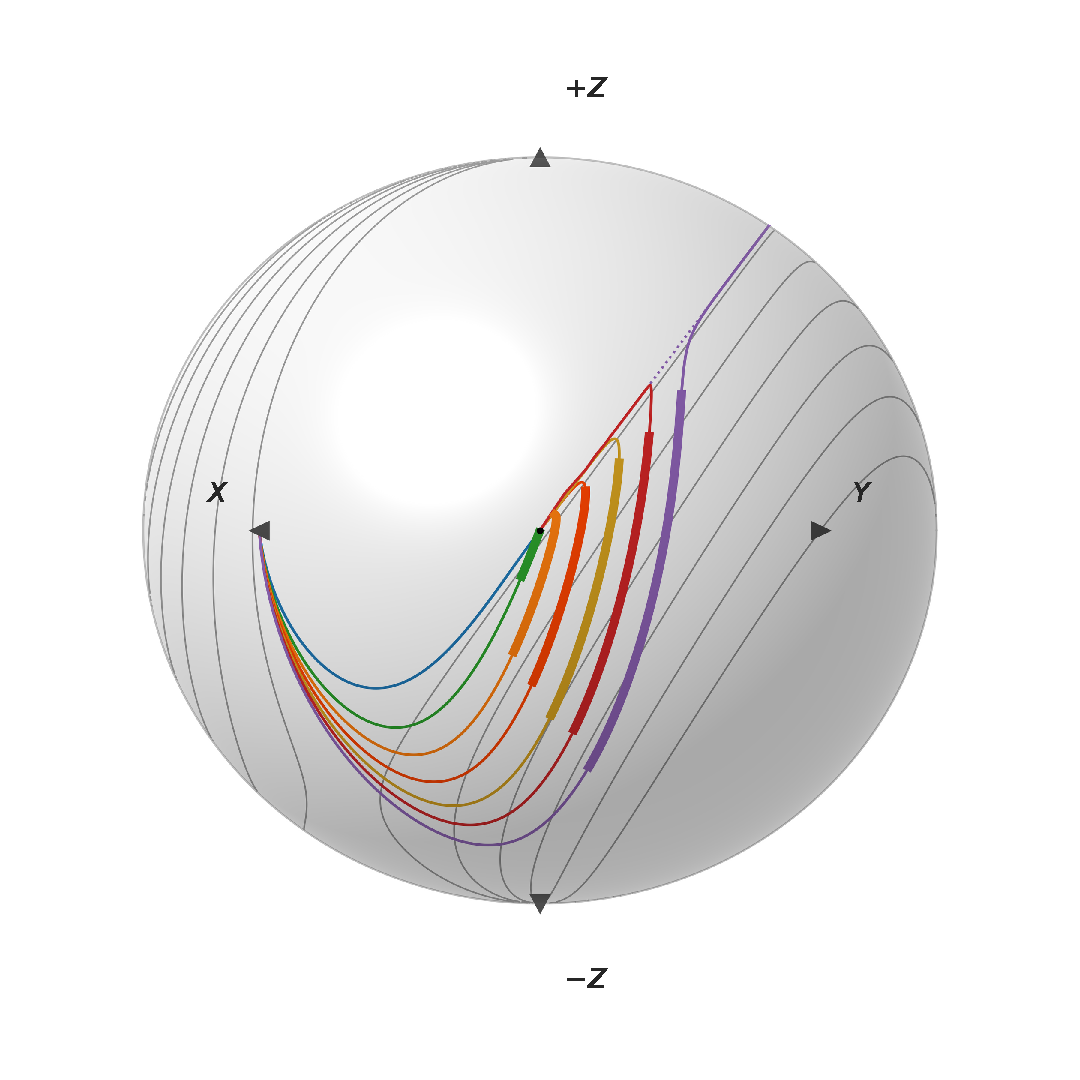
\includegraphics[width=0.68\textwidth]{indicator_sphere.pdf}
  \caption{The profiles the kernel must match, on the $\mathbb{RP}^2$ indicator
  sphere \eqref{eq:indicators} (orthographic x-ray view: curvature vertical,
  vorticity$-$velocity horizontal; near hemisphere solid, far side dotted;
  triangles mark the four visible poles---velocity left, vorticity right,
  $\pm$curvature top and bottom). Seven Falkner--Skan profiles run as thin
  curves from the wall (center) toward the freestream: favorable
  ($\beta\!=\!+0.30$, blue), Blasius ($\beta\!=\!0$, green), moderate
  adverse ($\beta\!=\!-0.10$, orange), strongly adverse
  ($\beta\!=\!-0.16$, red-orange), near-separation attached
  ($\beta\!=\!-0.19$, gold), incipient separation
  ($\beta\!=\!-0.1988$, red), and a separated reversed-flow shear
  layer---the Stewartson
  lower-branch solution at $\beta\!=\!-0.19$, $H\!\approx\!4.9$ (purple).
  The \textbf{thick} segment on each marks
  the wall-normal band where its linear-stability (Orr--Sommerfeld
  Reynolds-stress production) density exceeds half its peak---where the
  disturbance actually grows; the attached profiles are evaluated at
  $Re_\theta\!=\!500$ (the favorable layer is still subcritical there and
  carries no band), the reversed-flow profile at $Re_\theta\!=\!200$. Gray lines are contours of the rate coordinate
  $\hat\Omega \hat I$ at $\{0.025,0.2,0.4,0.6,0.8,1.0\}$.}
  \label{fig:model}
\end{figure}

The profiles of \S\ref{sec:reproduce} become curves on this sphere
(Fig.~\ref{fig:model}), and following one fixes the coordinate the rate will
need. Every profile begins at the same \emph{wall point}: the linear sublayer
$u\!\approx\!u'_w d$ makes velocity and shear equal, and although the curvature
$u''$ is finite there, its $d^2$ weight sends the indicator $Z\!\to\!0$, so the
state sits at $X\!=\!Y$, $Z\!=\!0$ (longitude $\lambda\!=\!45^\circ$, on the
equator). What every profile shares as it leaves is not a common direction but a
\emph{constraint}. To second order the near-wall profile is a parabola, and a
parabola $u=By+Cy^2$ satisfies, through \eqref{eq:indicators}, the single linear
relation
\begin{equation}
  \hat I \;\equiv\; Y - X - Z \;=\; \text{vorticity}-\text{velocity}-\text{curvature} \;=\; 0
  \label{eq:parabola}
\end{equation}
identically, so the parabola great circle $\hat I=0$ is the neutral locus. A real
profile matches its osculating parabola through second order; $\hat I$ and its first
two wall derivatives therefore vanish, and $\hat I$ departs zero only at third order
(a Taylor identity). The profiles do not all leave the wall point along the same
sphere-tangent---only those with wall curvature ($u''_w\!\neq\!0$, a
pressure-gradient effect) leave tangent to the circle, while a zero-gradient
layer, having $u''_w\!=\!0$, peels off at a small angle---but every one departs
with $\hat I$ third-order small. What distinguishes them is \emph{how they leave} that circle,
and a profile can leave it only through its third derivative: integrating
\eqref{eq:parabola} by parts against $u(0)=0$ gives, for the unnormalized
combination,
\begin{equation}
  I(d) \;\equiv\; R\,\hat I \;=\; d\,u' - u - \tfrac12 d^2 u''
  \;=\; -\int_0^d \tfrac12\,s^2\,u'''(s)\,\mathrm{d}s ,
  \label{eq:g_integral}
\end{equation}
so $I$ is exactly the residual of the near-wall parabolic fit: the
\emph{accumulated inflection}---the integrand
$-\tfrac12 s^2 u''' = \tfrac12 s^2\omega''$ is the third-derivative
contribution to the wall-to-point change of the vorticity, and $I$
accumulates it from the wall to the probe point. Since
$u'''\!=\!-\omega''$ (with the two-dimensional sign
convention $\omega=-u'$ used in this section; elsewhere $\omega$ denotes the
vorticity magnitude), it is the
accumulated curvature of the vorticity profile, the inflectional content
Rayleigh's theorem ties to inviscid instability~\cite{schmid_henningson_2001};
$\hat I>0$ marks the inflectional side.

Read against Fig.~\ref{fig:model}, the family orders itself by how its wall
curvature evolves, since \eqref{eq:g_integral} integrates the slope of that
curvature. The \emph{favorable} layer carries a negative wall curvature
($u''_w\!<\!0$) that only relaxes toward zero at the edge; its slope $u'''$ stays
positive, so $\hat I$ leaves the circle tangentially and dives at once to the stable
$\hat I\!<\!0$ side, never turning inflectional. \emph{Blasius} starts flat
($u''_w\!=\!0$): its curvature first builds up---dipping negative a short way off
the wall---before decaying back, so $u'''\!<\!0$ near the wall lifts $\hat I$ into a
small positive bump (the weak instability) before $u'''\!>\!0$ aloft draws it
down again. An \emph{adverse} gradient deepens and widens that curvature deficit,
and the $s^2$ weight and thicker layer amplify its contribution, so the bump
grows into a large positive hump: the adverse and incipient-separation profiles
sit well onto the inflectional ($+\hat I$) side. The \emph{separated} profile leaves
the wall the \emph{other} way (dotted, reversed flow) along the same parabola,
and along that arc it too is stable; but as it crosses the velocity-zero
longitude---the vorticity pole on the equator---$\hat I$ turns sharply positive, past even
the separation threshold, the most unstable member of the family. Every profile
finally settles at the \emph{velocity pole} ($X\!\to\!1$, $\hat I\!\to\!-1$) as the
shear dies at the edge; what distinguishes them is only the size of the positive
excursion in between.

\subsection{Where and how much the instabilities amplify}%
\label{sec:live}\label{sec:rate}\label{sec:calib_rate}\label{sec:nulamscale}
On each of these curves we thicken the wall-normal band where the disturbance
actually grows---the contiguous interval over which the most-unstable
Orr--Sommerfeld mode's production density
$\tfrac{\alpha_x}{2}\,|\mathrm{Im}(\phi'\phi^{*})|\,|U'|$ ($\alpha_x$ the
streamwise wavenumber) stays above half its
peak (the thick segments in Fig.~\ref{fig:model}). Two facts then read straight
off the plot. First,
\emph{every} amplifying band lies east of the velocity-pole longitude,
toward the vorticity pole $+Y$ and away from the pure-curvature poles. Second, the amplifying region is bounded below by exactly
the parabola great circle $\hat I=0$ of \eqref{eq:parabola}: a parabola being
inviscidly neutral by Rayleigh's theorem, $\hat I=0$ is the neutral boundary and
every band sits on the inflectional $\hat I>0$ side identified in
\S\ref{sec:sphere}. Where amplification can \emph{begin} follows from the same
integral \eqref{eq:g_integral}: the $s^2$ weight and the steady-wall
compatibility $u'''_w=0$~\cite{white_2006} start every profile at $\hat I=0$, tangent
to the neutral circle. This has two consequences. A layer reaches the
inflectional side only once accumulated curvature reversal carries it across
$\hat I=0$---the lower bound the bands of Fig.~\ref{fig:model} sit above. And because
the rate coordinate $\hat\Omega \hat I$ inherits $\hat I=0$ at the wall, the kernel produces nothing
there: amplification is held off the wall by construction, never seeded at the
no-slip line where the eddy viscosity vanishes. The growing region sits at a
viscous standoff fixed by the $Re_\Omega$ onset gate (\S\ref{sec:onset}), which
is what makes the inception Reynolds-number dependent even though the rate itself
is not.

The rate joins the two odd sphere functions---the vorticity fraction $\hat\Omega$ and
the accumulated-inflection coordinate $\hat I$---into their even product $\hat\Omega\,\hat I$, the single amplifying coordinate the projective algebra allows: positive on the
inflectional (shear) side, negative on the parabola's stable side, zero on the
neutral circle, and---being weighted by the longitude-only $\hat\Omega$---finite at
the curvature pole, so a detached shear layer standing off the wall still
registers. The rate is
\begin{equation}
  a \;=\; a_{\max}\,\operatorname{clip}\!\big\langle\, \hat\Omega\,\hat I\,\big\rangle_{0}^{1},
  \qquad
  \operatorname{clip}\langle x\rangle_{0}^{1} \;=\; \min\!\big(\max(x,0),\,1\big),
  \label{eq:rate}
\end{equation}
linear in the even product, with $a_{\max}$ the free-shear ceiling (fixed just
below), reached where $\hat\Omega \hat I\!\ge\!1$ at the vorticity pole ($\hat\Omega\!\to\!1$, the
free-shear-layer limit). No
near-neutral shaping is needed: measured against the Drela--Giles envelope,
the linear rate tracks it across the attached shape-factor family, softening
only at the separation edge (below). Because a favorable gradient keeps the profile's curvature
single-signed (the accumulated curvature reversal that carries a layer
across the neutral circle never builds), $\hat\Omega \hat I\!\to\!0$ on the
favorable side and the
rate vanishes with it; no
separate suppression term is needed.

The prefactor $a_{\max}$ is a natural physical limit, set by the structure of
the amplification itself. To
the accuracy of the $e^N$ method, the envelope amplification a profile earns per
unit $Re_\theta$ is a function of its shape alone---Reynolds-%
independent~\cite{drela_giles_1987}. The canonical layers therefore form a
single shape-driven continuum: from the near-parabolic Blasius profile, through
the adverse layers as an inflection point emerges and the growth turns inviscid
(Rayleigh), to the detached shear layer of a separation bubble and its unbounded
limit, the free mixing layer. The coordinate $\hat\Omega \hat I$ runs along exactly this
continuum---zero on the neutral parabola, unity at the fully-inflectional
vorticity pole---so one ceiling closes it.

At that pole the profile \emph{is} a free shear layer, and its amplification is
the inviscid Kelvin--Helmholtz instability: a \emph{temporal} eigenvalue with no
free constant. For the hyperbolic-tangent layer the most-amplified mode grows at
$\omega_{i,\max}=0.1897\,U_0/\delta$ against a peak vorticity
$\omega_{\mathrm{peak}}=U_0/\delta$~\cite{michalke_1964}, a ratio independent of
the velocity and thickness normalization, so
\begin{equation*}
  a_{\max} \;=\; \omega_{i,\max}/\omega_{\mathrm{peak}} \;=\; 0.19 ,
\end{equation*}
an eigenvalue---the head of the continuum. The model grows
$\tilde\nu$ along particle paths at $a(\hat\Omega \hat I)\,\omega$, a
\emph{temporal} rate that convection lays down as the spatial $N$-factor
(Eq.~\eqref{eq:pai_def}): the same temporal-to-spatial passage that connects a
growth eigenvalue to an accumulated amplification.

How well does the closed rate hold up, quantitatively, against the
correlation it must reproduce? The comparison can be made analytically,
before any transport equation is solved. Hold a Falkner--Skan profile
frozen and parallel: a disturbance riding it grows at $a(\hat\Omega \hat I)\,\omega$
while it advects at the local $u$, so the growth the rate can hand the
transport per unit length---before any viscous loss---is the pointwise
supremum $\max_y a\,\omega/u$. Drela's envelope correlation states the
same quantity as an explicit spatial rate, $s_{\mathrm{DG}}/\theta$ with
$s_{\mathrm{DG}}\!=\!\tfrac{m(H)+1}{2}\,\ell(H)\,\mathrm dN/\mathrm dRe_\theta$
($\ell$, $m$ the Falkner--Skan similarity factors of Drela's spatial
conversion~\cite{drela_giles_1987}), so the two compare with no wave-speed
convention on either side. Table~\ref{tab:ratelimit} lists the ratio
across the family---which stops at $H\!\approx\!5$, where Drela's
Orr--Sommerfeld data end and no similarity profile remains validated
against measured bubble profiles---and two facts read off it. Across the attached
branch the inviscid slope rides a nearly uniform $1.30$--$1.42\times$
above the correlation---headroom, and what consumes it is the subject of
the next paragraphs. At the separation limit and onto the
shallow reversed-flow branch the ratio is $0.97$.

\begin{table}[tp]
  \centering
  \small
  \caption{The inviscid frozen-profile slope of the rate \eqref{eq:rate},
  $\max_y a\,\omega/u$, as a ratio to the Drela--Giles spatial envelope
  rate $s_{\mathrm{DG}}/\theta$, on five Falkner--Skan profiles (starred:
  the reversed-flow, Stewartson lower-branch solution of the same
  $\beta$). $\max_y\hat\Omega \hat I$ is each profile's peak rate coordinate---the
  scale the airfoil visualizations of
  Secs.~\ref{sec:nlfval}--\ref{sec:eppval} are read against. The ratio is
  independent of Reynolds number and of any diffusion: it is the most
  growth per unit length the rate can sustain on the profile. The
  diffusion retained by the working variable, taken up next, lowers the
  realized slope toward and below these values at transitional Reynolds
  numbers (Table~\ref{tab:frozeneig}).}
  \label{tab:ratelimit}
  \begin{tabular}{lrrrc}
    \toprule
    profile & $\beta$ & $H$ & $\max_y \hat\Omega \hat I$ & $\theta\,\max_y(a\,\omega/u)\;/\;s_{\mathrm{DG}}$\\
    \midrule
    moderate favorable & $+0.10$ & 2.48 & 0.037 & 1.30\\
    Blasius & $0$ & 2.59 & 0.078 & 1.42\\
    moderate adverse & $-0.10$ & 2.80 & 0.162 & 1.30\\
    separation limit & $-0.1988$ & 3.98 & 0.510 & 0.97\\
    separated, shallow$^\ast$ & $-0.19$ & 4.92 & 0.657 & 0.97\\
    \bottomrule
  \end{tabular}
\end{table}

The headroom is spent on viscosity. The working variable that carries the
disturbance lives in the SA equation \eqref{eq:sa}, and it diffuses with
the molecular coefficient all the while it grows. On the frozen profile
the contest is an eigenvalue problem: growth, diffusion, and advection
compose the generalized problem
\begin{equation}
  \Bigl[\,a(\hat\Omega \hat I)\,\omega
  \;+\;\frac{c_{\nu,\mathrm{ai}}\,\nu}{\sigma}\,\partial_y^2\Bigr]\,v
  \;=\; s\,u\,v,
  \label{eq:frozeneig}
\end{equation}
whose leading eigenvalue $s$ is the growth per unit length the transport
can actually realize on that profile at that Reynolds number---the
inviscid supremum of Table~\ref{tab:ratelimit} recovered as
$Re_\theta\!\to\!\infty$, approached like $Re_\theta^{-1/2}$ as the
eigenfunction narrows onto its peak. The problem is well posed and cheap:
$v\!=\!0$ at the wall and the far field, the reversed-flow advection
floored at $0.02\,U_e$ (a choice the result is insensitive to: floors
$0.01$--$0.05\,U_e$ move no printed digit), and the substitution
$v\!\to\!u^{-1/2}v$ then makes the operator symmetric, so each entry
below is one symmetric tridiagonal eigenvalue. Here
$c_{\nu,\mathrm{ai}}$ is a scale on the molecular coefficient, equal to
one until decided otherwise. Table~\ref{tab:frozeneig} carries the
result, at the stations where each profile is unstable by the
Drela--Giles criterion ($Re_\theta\!>\!Re_{\theta 0}(H)$, third column):
below its critical Reynolds number a profile earns no envelope growth,
and there is nothing to compare against. With the
coefficient untouched ($c_{\nu,\mathrm{ai}}\!=\!1$, left half), the
equation declines the correlation everywhere the family grows: half of
Drela's slope just past the Blasius critical station ($0.49$ at
$Re_\theta\!=\!400$), $0.63$ at the favorable wedge's lone unstable
station, and $0.64$--$0.85$ even on the separation branch, where
diffusion should matter least. At full molecular
diffusion the drain does not perturb the growth; it overwhelms it.

So we let the disturbance keep less of it. The laminar viscosity in the
SA diffusion term---and only there---is scaled by a constant factor
$c_{\nu,\mathrm{ai}}\!<\!1$,
\begin{equation}
  (\nu+\tilde\nu)\;\longrightarrow\;(c_{\nu,\mathrm{ai}}\,\nu+\tilde\nu)
  \quad\text{in the diffusion term of Eq.~\eqref{eq:sa} only,}
  \label{eq:nulamscale}
\end{equation}
leaving the mean-flow viscosity, the SA production and destruction, and the
definition $\chi=\tilde\nu/\nu$ (formed with the \emph{true} $\nu$)
untouched. Doing so barely disturbs the original SA calibration---the
scaling multiplies a term that is negligible or exactly zero wherever
that calibration acts, quantified in Sec.~\ref{sec:calib_diff}. How much
less, the eigenvalue decides, read against a
constraint that pulls the other way. Halving the coefficient down the
ladder $c_{\nu,\mathrm{ai}}=1,\tfrac12,\tfrac13,\tfrac16,\tfrac1{12}$,
the station just past the Blasius critical station ($Re_\theta\!=\!400$) climbs
$0.49$, $0.75$, $0.87$, $1.02$, $1.13$: the growth arrives on the
correlation at $\tfrac16$ and overshoots past it. The family arrives
together---the favorable wedge's lone unstable station reads $1.02$ at
the same $\tfrac16$, and the moderate adverse crosses unity between
$\tfrac13$ and $\tfrac16$ ($1.04$ at $Re_\theta\!=\!400$). Pressing
further toward the inviscid ceiling would demand ever more grid
resolution: the molecular floor sets
the smallest wall-normal scale the $\tilde\nu$ field can develop, the
equilibrium band thickness scaling as $\sqrt{c_{\nu,\mathrm{ai}}}$, so
every halving thins the disturbance band the mesh must resolve by
$\sqrt2$. We stop at
\begin{equation*}
  c_{\nu,\mathrm{ai}} \;=\; \tfrac{1}{6},
\end{equation*}
where the just-past-critical stations sit on the correlation and the
separation branch holds $0.82$--$0.91$ (right half of
Table~\ref{tab:frozeneig}); what remains is a mild drift above it later
in each profile's unstable decade (Blasius $1.21$ by
$Re_\theta\!=\!1600$, where transition on that layer is already
complete), climbing toward the finite ceiling of
Table~\ref{tab:ratelimit} as the diffusion keeps vanishing. The
negative-$\tilde\nu$ safeguards~\cite{allmaras_2012} carry over with one
consistency requirement: the negative-branch factor $f_n$ is formed with
the scaled coefficient $c_{\nu,\mathrm{ai}}\,\nu$, which keeps the total
diffusivity positive, $c_{\nu,\mathrm{ai}}\nu + f_n\tilde\nu\!>\!0$.

\begin{table}[tp]
  \centering
  \small
  \caption{The frozen-profile eigenvalue of Eq.~\eqref{eq:frozeneig}---the
  growth per unit length the transport realizes with diffusion
  retained---as a ratio to the Drela--Giles rate $s_{\mathrm{DG}}/\theta$
  across the transitional decade $Re_\theta=200$--$1600$, at the untouched
  molecular coefficient ($c_{\nu,\mathrm{ai}}\!=\!1$) and at the adopted
  $c_{\nu,\mathrm{ai}}\!=\!\tfrac16$. Profiles are identified by their
  peak rate coordinate $\max_y\hat\Omega \hat I$ (the $\beta$ map is
  Table~\ref{tab:ratelimit}). Entries appear only at stations
  above the profile's Drela--Giles critical Reynolds number
  $Re_{\theta 0}(H)$ (third column): where the profile is stable, the
  correlation has no growth to compare against. Each entry is one
  symmetric tridiagonal eigenvalue ($u^{1/2}$ similarity; $v\!=\!0$ at
  the wall and the far field; reversed-flow advection floored at
  $0.02\,U_e$, floors $0.01$--$0.05$ moving no printed digit). The
  starred row is the reversed-flow (Stewartson lower-branch) solution at
  $\beta\!=\!-0.19$; the $Re_\theta\!\to\!\infty$ limit of every row is
  Table~\ref{tab:ratelimit}.}
  \label{tab:frozeneig}
  \begin{tabular}{lrr cccc cccc}
    \toprule
    & & & \multicolumn{4}{c}{$c_{\nu,\mathrm{ai}}=1$}
      & \multicolumn{4}{c}{$c_{\nu,\mathrm{ai}}=1/6$}\\
    \cmidrule(lr){4-7}\cmidrule(lr){8-11}
    profile & $\max_y \hat\Omega \hat I$ & $Re_{\theta 0}$ & $200$ & $400$ & $800$ & $1600$
                      & $200$ & $400$ & $800$ & $1600$\\
    \midrule
    moderate favorable & $0.037$ & $827$ & -- & -- & -- & $0.63$
                                 & -- & -- & -- & $1.02$\\
    Blasius            & $0.078$ & $242$ & -- & $0.49$ & $0.75$ & $0.94$
                                 & -- & $1.02$ & $1.13$ & $1.21$\\
    moderate adverse   & $0.162$ & $97$ & $0.50$ & $0.72$ & $0.87$ & $0.99$
                                 & $0.94$ & $1.04$ & $1.11$ & $1.16$\\
    separation limit   & $0.510$ & $36$ & $0.64$ & $0.72$ & $0.79$ & $0.83$
                                 & $0.82$ & $0.86$ & $0.89$ & $0.91$\\
    separated, shallow$^\ast$ & $0.657$ & $26$ & $0.68$ & $0.75$ & $0.80$ & $0.85$
                                 & $0.83$ & $0.87$ & $0.89$ & $0.91$\\
    \bottomrule
  \end{tabular}
\end{table}

What the rate and its retained diffusion do not set is where the growth
may \emph{begin}. A laminar layer does not amplify from birth: linear
theory gives each shape a floor, the critical Reynolds number
$Re_{\theta 0}(H)$ below which every disturbance decays (the third
column of Table~\ref{tab:frozeneig}), and growth starts only past it.
The frozen profile of Eq.~\eqref{eq:frozeneig} knows no such floor:
growth beats the drain from $Re_\theta$ of a few tens
($\approx\!20$ on Blasius at the adopted coefficient)---far below the
physical floor---so the laminar regime cannot be held by the drain
alone: the inception is a threshold of its own, and it is the subject of
the next subsection.

\subsection{The onset threshold}%
\label{sec:onset}\label{sec:calib_onset}
In the $e^N$ envelope description a laminar layer amplifies in two
regimes: nothing grows until the layer reaches a shape-dependent
critical Reynolds number $Re_{\theta 0}(H)$, and past it the envelope
earns amplification at a rate that is, to the accuracy of the method,
Reynolds-independent---a function of the shape
alone~\cite{drela_giles_1987}. The algebraic rate \eqref{eq:rate}
carries the second regime and no explicit Reynolds number; the
first---the viscous inception---is a separate,
multiplicative gate on the vorticity Reynolds number, rising smoothly from $0$
to $1$,
\begin{equation}
  S\!\big(Re_\Omega / Re_\Omega^{\mathrm c}(\hat\Omega \hat I)\big),
  \qquad S(\zeta) = \tfrac12\big[1+\tanh\!\big((\zeta-1)/w\big)\big],
  \qquad Re_\Omega = d^2\omega/\nu ,
  \label{eq:onset}
\end{equation}
with $w$ the onset ramp width scale and
its threshold a function of the \emph{same} product $\hat\Omega \hat I$ (the form
\eqref{eq:reomc}, fixed below). The width is not a fitted quantity. We
set $w\!=\!0.35$---the gate runs from $12\%$ to $88\%$ open as
$Re_\Omega$ crosses from $0.65$ to $1.35$ of its threshold---and the
model barely notices: along a growing layer the vorticity Reynolds
number sweeps through the ramp quickly ($Re_\Omega$ grows like
$Re_\theta^2$ at fixed shape), so the marched $N\!=\!1$ stations of the
family (Sec.~\ref{sec:calib_onset}) move by under $1\%$ when $w$ is
halved and under $2.5\%$ when it is doubled, shifts the anchor absorbs.
A smooth ramp of finite width is still the right form: linear-stability
onset is itself not sharp (the graze scatter below is $6$--$14\%$), and a
near-discontinuous source is hostile to the coupled solver's meshes and
Newton convergence. Rate and onset reinforce: near the
parabola a low rate \emph{and} a high threshold give the late, slow transition
of a zero-pressure-gradient layer; inflectional profiles get a high rate
\emph{and} a low threshold, hence early, fast transition. The complete source
is
\begin{equation}
  P_{\mathrm{AI}} \;=\; a_{\max}\,\operatorname{clip}\!\big\langle \hat\Omega \hat I\,\big\rangle_{0}^{1}\;
  S\!\big(Re_\Omega/Re_\Omega^{\mathrm c}(\hat\Omega \hat I)\big)\;\omega\,\tilde\nu .
  \label{eq:pai}
\end{equation}
Two functions of the one even coordinate $\hat\Omega \hat I$---the rate and the onset
threshold---carry the whole model. A favorable gradient drives
$\hat\Omega \hat I\!\to\!0$, so both shut off geometrically, with no pressure-gradient
parameter anywhere.

\begin{figure}[tp]
  \centering
  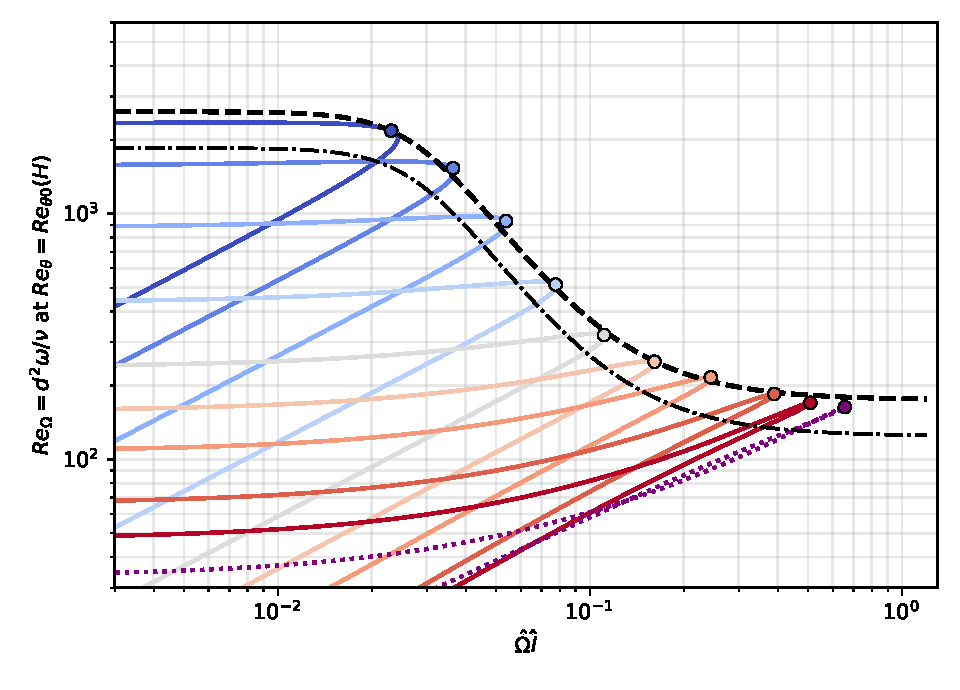
\includegraphics[width=0.62\textwidth]{onset_graze.pdf}
  \caption{The onset threshold's shape from the linear-stability graze. Each
  Falkner--Skan profile, at its Drela--Giles critical Reynolds number
  $Re_{\theta 0}(H)$, traces a curve in the $(\hat\Omega \hat I,\,Re_\Omega)$ plane:
  solid, colored blue to red with decreasing $\beta$, the attached family
  $\beta = +0.15$, $+0.10$, $+0.05$, $0$ (Blasius), $-0.05$,
  $-0.10$, $-0.15$, $-0.19$, $-0.1988$ (incipient separation); dotted, a
  separated reversed-flow profile, the Stewartson lower-branch solution at
  $\beta\!=\!-0.19$ ($H\!\approx\!4.9$). The attached family
  shares the dashed outer envelope, which each member grazes at its marked
  closest-approach point: graze ratios $0.93$--$1.14$ (root-mean-square
  $\sim\!6\%$) from incipient separation through $\beta=+0.15$. The
  soft-min
  shape of Eq.~\eqref{eq:reomc}, at $k\!=\!1$, is that envelope: a ceiling on the favorable
  (small $\hat\Omega \hat I$) side, an additive floor toward separation; dash-dot,
  the model threshold---the same shape scaled by the calibrated
  $k\!=\!0.712$ of the march anchor below.}
  \label{fig:onsetgraze}
\end{figure}

The one free function is the onset threshold $Re_\Omega^{\mathrm c}(\hat\Omega \hat I)$ of the
gate \eqref{eq:onset}, and its \emph{shape} follows from linear theory.
Figure~\ref{fig:onsetgraze} makes the construction concrete. Each attached
Falkner--Skan profile, evaluated at its Drela--Giles critical Reynolds number
$Re_{\theta 0}(H)$---the station where the layer first turns linearly
unstable---traces a curve in the $(\hat\Omega \hat I,\,Re_\Omega)$ plane, and the family
shares a common outer envelope: a threshold curve that each profile
\emph{grazes}, touching without crossing, at its own most-critical point. The
graze collapses the family onto one monotone shape. On the favorable side the
threshold saturates toward a ceiling---an accelerated layer must grow thicker
before any point of it turns critical, but not indefinitely so---while near
separation it flattens onto an additive floor, inception becoming essentially
immediate. The collapse does not stop at the separation limit: the
reversed-flow profile grazes the same envelope at its own critical
Reynolds number, and because that critical value is tiny
($Re_{\theta 0}\!\approx\!26$), at any Reynolds number a bubble actually
reaches the profile rides far above the floor and ignites at once, as it
should.
We represent the shape by a soft minimum of the two limits,
\begin{equation}
  Re_\Omega^{\mathrm c}(\hat\Omega \hat I) \;=\; k\,\operatorname{softmin}_2\!\Big(C,\;
      A + B\,\langle\hat\Omega \hat I\rangle_+^{-2}\Big),
  \qquad (C,\,A,\,B) \;=\; (2600,\;175,\;2),
  \label{eq:reomc}
\end{equation}
with $\operatorname{softmin}_2(x_1,x_2)\!=\!x_1 x_2/\sqrt{x_1^2+x_2^2}$; the
graze fixes the three shape constants to a root-mean-square graze error of
$\sim\!6\%$ from incipient separation through $\beta\!=\!+0.15$ (the
soft-min exponent $2$ is the best of the sharpnesses tried), and they are
never refit; strongly favorable members ($\beta\!\geq\!+0.25$, beyond
the plotted family) graze
$1.27$--$1.34$ high, consistent with the favorable-branch departure the
calibration will meet below.

That leaves the single scale $k$, and its role is physical. Linear theory
knows only the profile; the working variable that must carry the
amplification also \emph{diffuses}, with the retained molecular
coefficient $c_{\nu,\mathrm{ai}}\nu$ of Sec.~\ref{sec:nulamscale}, all
the while it grows. The drain is felt most where inception
happens at low Reynolds number---in a thin layer the young disturbance loses
to viscosity for a while after the model first lets its growth rate turn
positive, so
net growth starts late. The compensation is to permit inception
\emph{earlier} than the inviscid graze: one factor $k\!<\!1$ scales the
whole threshold, so that the accumulated growth reaches the correlation's
first station on time. Its size has to be measured, with the model's
own equation marched down the layer.

The simplest such instrument is a parabolized march of that equation:
in non-dimensional boundary-layer variables (length in $\nu/U_\infty$,
velocity in $U_\infty$),
\begin{equation}
  u\,\frac{\partial\hat\nu}{\partial x} + v\,\frac{\partial\hat\nu}{\partial y}
  = \frac{c_{\nu,\mathrm{ai}}}{\sigma}\,\frac{\partial^2\hat\nu}{\partial y^2}
    + a(\hat\Omega \hat I)\,S\!\big(Re_\Omega/Re_\Omega^{\mathrm c}(\hat\Omega \hat I)\big)\,\omega\,\hat\nu,
  \label{eq:transport}
\end{equation}
keeping the amplification and the molecular part of the SA cross-stream
diffusion. The $\tilde\nu\,\nabla^2\tilde\nu$ self-diffusion and $c_{b2}$
gradient terms are $O(\chi)$ smaller in this range and are dropped,
in the manner of the classical parabolized boundary-layer
equations~\cite{white_2006}. No SA
production or destruction enters: production is switched off outright
where $\chi\!\le\!1$ ($\sigma_P\!=\!0$, Sec.~\ref{sec:blend}), and the
tied destruction floor is inert at the disturbance's scale ($<10^{-3}$
of the amplification, same section). The
march is seeded
at the leading edge with one unit of an arbitrary infinitesimal: the
equation is linear in $\hat\nu$, so the seed's magnitude cancels from
every ratio and only the accumulated growth is meaningful. Measured in
that unit, $N\!=\!\ln\hat\nu$ is the
amplification factor by construction, and its envelope can be laid directly
against Drela--Giles~\cite{drela_giles_1987}. (The crossings quoted in this
subsection are grid-converged values of the march; the $N\!=\!1$ crossing in
particular demands a fine wall-normal grid, the amplifying band being thin
where inception occurs.)

\begin{figure}[tp]
  \centering
  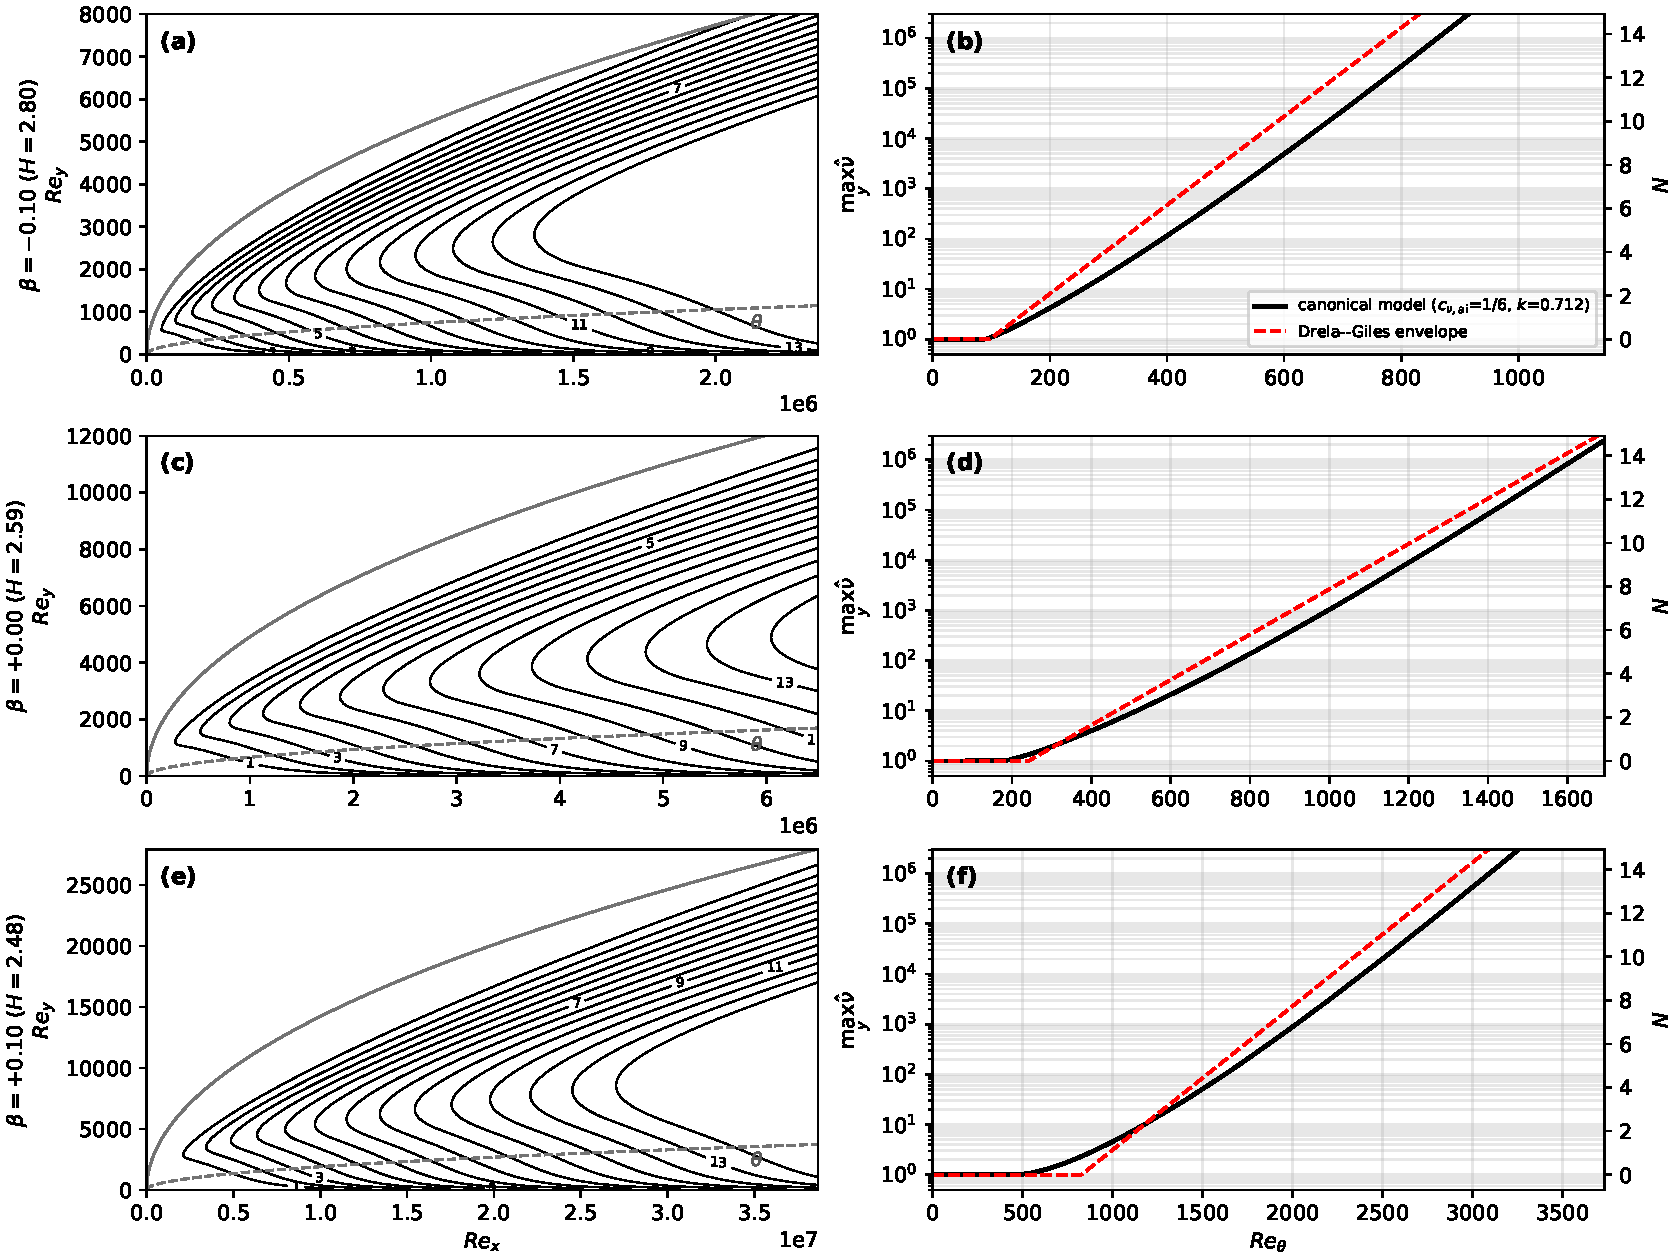
\includegraphics[width=0.99\textwidth]{fs_nuHat_rows.pdf}
  \caption{The disturbance transport \eqref{eq:transport} on three wedge
  flows---adverse ($\beta\!=\!-0.10$, top), Blasius ($\beta\!=\!0$, middle:
  the calibration anchor), and mildly favorable ($\beta\!=\!+0.10$,
  bottom; $\max_y\hat\Omega \hat I=0.162$, $0.078$, and $0.037$,
  respectively)---seeded
  $\hat\nu_\infty\!=\!1$, $a_{\max}=0.19$.
  \textbf{Left column} (a,c,e): contours of $N\!=\!\ln\hat\nu$ at the
  canonical $(c_{\nu,\mathrm{ai}},k)=(\tfrac16,\,0.712)$ in the
  local-Reynolds plane, concentrated between the overlaid
  momentum thickness $\theta$ (dashed) and edge thickness $\delta_{99}$
  (solid) where the amplifying band sits. \textbf{Right column} (b,d,f): the
  marched envelope $\max_y\hat\nu$ vs $Re_\theta$ (log left axis; $N$ linear
  right axis) at the canonical
  $(c_{\nu,\mathrm{ai}},k)=(\tfrac16,\,0.712)$ (black), against each
  profile's Drela--Giles
  envelope~\cite{drela_giles_1987} (red dashed). On the anchor (d) the
  canonical envelope meets the correlation at $N\!=\!1$ by construction
  (Sec.~\ref{sec:calib_onset}); its $N\!=\!9$ crossing is an untuned
  prediction, $7\%$ past Drela's. The adverse wedge (b) ignites earlier and
  grows faster. The mildly favorable wedge (f) stays close to the
  correlation---its $N\!=\!1$ station lands ${\sim}11\%$ early---with the
  suppressed rate stretching the growth over a run nearly twice
  Blasius's in $Re_\theta$ (over four times in $Re_x$), and no
  pressure-gradient parameter anywhere. A
  physical case seeded with $\chi_\infty$ hands over where its envelope
  crosses $N_\mathrm{crit}=\ln(c_{v1}/\chi_\infty)$ ($\chi\!=\!c_{v1}$; the
  seed convention of Sec.~\ref{sec:flatplate}).}
  \label{fig:nuhat}
\end{figure}

Marching the equation untouched
($c_{\nu,\mathrm{ai}}\!=\!1$, $k\!=\!1$) on the wedges of
Fig.~\ref{fig:nuhat} confirms the eigenvalue's
verdict of Sec.~\ref{sec:nulamscale} in accumulated form (not
plotted): the envelope
falls far short of the correlation, its early secant (the
$N\!\in\![1,5]$ span of the Blasius layer) running $24\%$ below the late
one ($N\!\in\![5,9]$), where the envelope's own curvature---the
$c_{\nu,\mathrm{ai}}\!\to\!0$ limit of the same march---is under $1\%$.
The march also adds what the asymptotic eigenvalue cannot see: at full
molecular diffusion the \emph{inception} fails outright, the Blasius
$N\!=\!1$ crossing sitting at $Re_\theta\!=\!392$ even with the threshold
removed entirely ($k\!\to\!0$)---the drain, not the threshold, sets the
inception, and no compensation exists. At the committed
$c_{\nu,\mathrm{ai}}\!=\!\tfrac16$ the drain is light enough that the
threshold is back in command, and $k$ has a value to take.

The compensation takes its value from a single anchor, stated
operationally: $k$ is chosen so
that the march \eqref{eq:transport}, on the Blasius layer at the committed
$c_{\nu,\mathrm{ai}}\!=\!\tfrac16$, crosses $N\!=\!1$ at the Drela--Giles
station $Re_\theta\!=\!338$; this gives $k\!=\!0.712$---the threshold
permitting inception $29\%$ earlier than the inviscid graze, the drain
consuming the difference.

Everything after that anchor is prediction. The marched Blasius envelope's
$N\!=\!9$ crossing lands at $Re_\theta\!=\!1181$, $7\%$ past Drela's
$1108$---the residual footprint of the retained diffusion (the late-envelope
slope itself matches Drela's to a fraction of a percent; the offset is
accumulated in the early, drain-affected span). Across the attached family
the $N\!=\!1$ stations land on the Drela--Giles stations to $6\%$
root-mean-square: the adverse wedges within $\pm4\%$, the favorable pair
$11$--$12\%$ early (Fig.~\ref{fig:calibrate}b)---the graze shape, anchored at
one point, carrying the family's two-decade threshold variation.

\begin{figure}[tp]
  \centering
  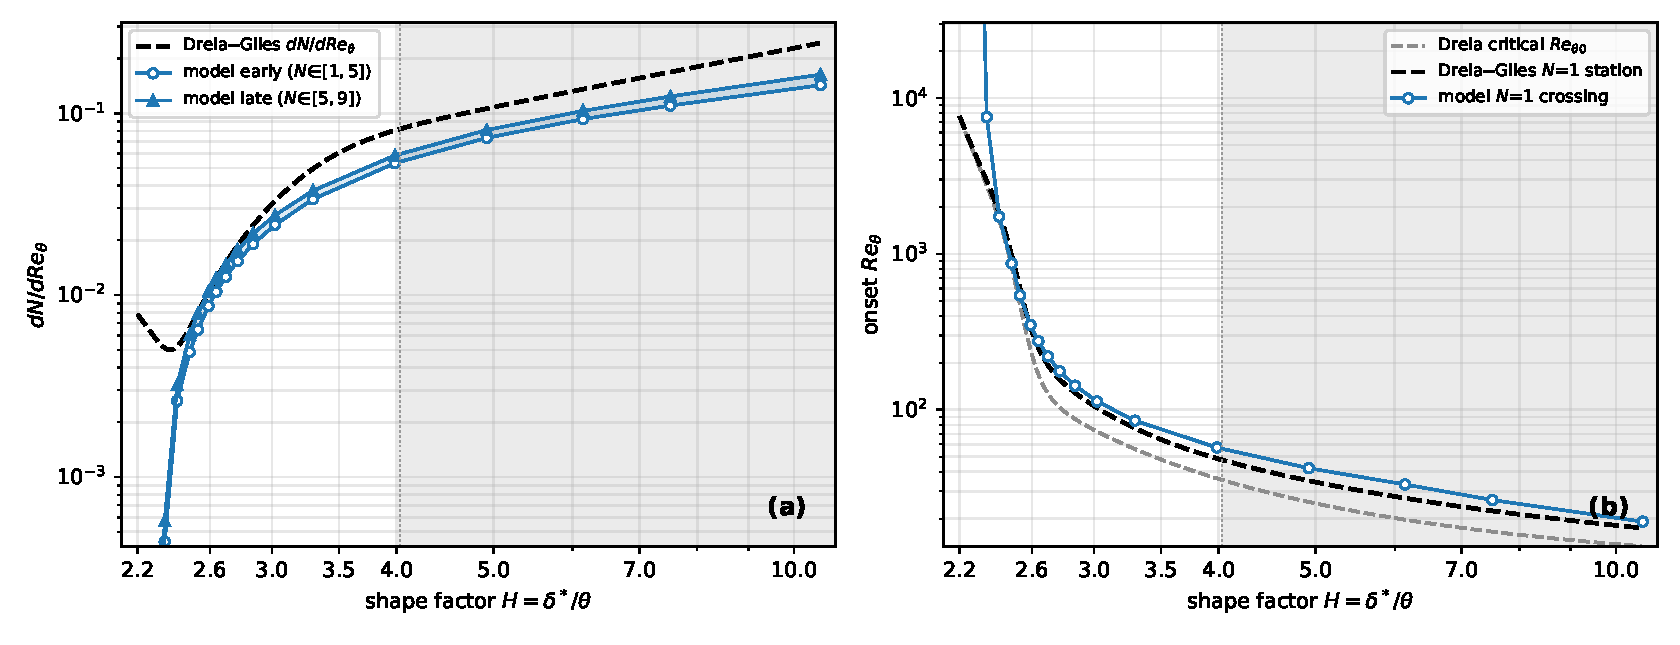
\includegraphics[width=\textwidth]{model_calibrate.pdf}
  \caption{The calibrated model compared with the Drela--Giles envelope
  across the full Falkner--Skan family, from the stagnation profile
  ($H\!\approx\!2.2$) through Blasius ($H\!\approx\!2.59$) and the separation
  limit ($H\!=\!3.98$, dotted) onto the reversed-flow (Stewartson lower)
  branch ($H\!\approx\!10.6$; separated region shaded). (a)~model rate
  $\mathrm dN/\mathrm dRe_\theta$ as an early ($N\!\in\![1,5]$) and a late
  ($N\!\in\![5,9]$) secant, band shaded---set entirely by the fixed
  eigenvalue $a_{\max}\!=\!0.19$ and $c_{\nu,\mathrm{ai}}\!=\!1/6$, with
  nothing tuned to this curve.
  (b)~model onset $Re_\theta$ (the $N\!=\!1$ crossing) against the
  Drela--Giles $N\!=\!1$ station $Re_{\theta 0}+1/(dN/dRe_\theta)$:
  anchored at Blasius,
  tracking the stations within ${\sim}\pm12\%$ across the attached
  family, from $H\!=\!2.44$ ($\beta\!=\!+0.15$) to $H\!=\!3.98$ (the
  separation limit).
  Both vertical axes extend slightly past the Drela range to show the
  favorable-regime departure---the rate falling below, the onset rising
  above---before the curves leave the panels.}
  \label{fig:calibrate}
\end{figure}

With $a_{\max}$ and the threshold both fixed, the marched envelope tracks
Drela--Giles across the attached family and softens through the separation limit
onto the reversed-flow branch (Fig.~\ref{fig:calibrate}a); the softening is
structural---the amplifying band thins as the profile approaches full
inflection, so the integrated envelope falls below the pointwise rate. The
favorable branch is where the model degrades, and the rate coordinate
grades the degradation (Fig.~\ref{fig:calibrate}). At
$\max_y\hat\Omega \hat I\!\approx\!0.04$ ($\beta\!=\!+0.10$, the bottom row of
Fig.~\ref{fig:nuhat}) the model is still roughly right, the marched
$N\!=\!1$ station ${\sim}11\%$ early; the family holds that level through
$\max_y\hat\Omega \hat I\!\approx\!0.02$ ($\beta\!=\!+0.15$). Beyond, the rate falls
faster than Drela's and the onset climbs above the critical Reynolds
number: by $\max_y\hat\Omega \hat I\!\approx\!2\!\times\!10^{-3}$
($\beta\!=\!+0.35$, $H\!\approx\!2.34$) the rate is
$\approx\!0.1\times$ Drela and the onset $\approx\!3\times$ its critical
$Re_\theta$; by $\beta\!\approx\!0.45$
($\max_y\hat\Omega \hat I\!\approx\!5\!\times\!10^{-4}$) transition has retreated beyond any
station of practical relevance (the marched $N\!=\!1$ station past
$Re_\theta\!\sim\!5\!\times\!10^5$), and stronger favorable wedges are
suppressed outright. The linear $\hat\Omega \hat I$ has no
near-neutral floor to hold the small favorable growth Drela's envelope keeps;
matching the strongly favorable branch is left to future work.

\subsection{The blend and its handover}\label{sec:blend}
A handover weight ties the laminar and turbulent regimes to the single state
variable through $\chi$,
\begin{equation}
  \sigma_t(\chi;\tau) = \max\!\left[\,1-e^{-(\chi-1)/\tau},\;0\right] \;=\;
  \begin{cases} 0, & \chi \le 1, \\ 1-e^{-(\chi-1)/\tau}, & \chi > 1. \end{cases}
  \label{eq:sigma}
\end{equation}
The
production and destruction of Eq.~\eqref{eq:sa} are blended, the production
with a width of its own, the destruction tied to it,
\begin{equation}
  P = \max\!\big[(1-\sigma_P)\,P_\mathrm{AI},\;\sigma_P\,P_\mathrm{SA}\big], \qquad
  D = \sigma_D\,D_\mathrm{SA}, \qquad
  \sigma_P = \sigma_t(\chi;\tau), \quad
  \sigma_D = 1-\frac{c_{b1}}{\kappa^2c_{w1}}\,(1-\sigma_P).
  \label{eq:blend}
\end{equation}
The $\max$ hands the production from amplification to SA at the
crossover: for $\chi\!\le\!1$ ($\sigma_P\!=\!0$) it returns $P_\mathrm{AI}$,
leaving the $e^N$ amplification unchanged, and once $\sigma_P P_\mathrm{SA}$
overtakes it just past $\chi\!=\!1$ the source reverts to standard SA with no
laminar residue. The production width $\tau$ is chosen for numerics
rather than physics, and is bracketed by its failure modes: too wide
throttles the SA production past $\chi\!=\!c_{v1}$, where the eddy
viscosity is already dynamically active; too narrow snaps to full SA at
$\chi\!=\!1$, compressing the transition zone into a front steeper than
the streamwise mesh can resolve. $\tau\!=\!4$ sits between them---the
handover is $78\%$ complete where $f_{v1}$ is half active
($\chi\!=\!c_{v1}$) and $97\%$ complete where $f_{v1}$ reaches $90\%$
($\chi\!\approx\!14.8$).
The destruction is not gated off but \emph{tied}, and needs no width of
its own: $\sigma_D$ tracks
$\sigma_P$ with slope $c_{b1}/(\kappa^2c_{w1})\!\approx\!0.249$ from the
floor $(1+c_{b2})/(\sigma c_{w1})\!\approx\!0.751$, the two summing to one
by the definition of $c_{w1}$. The tie is the weighting under which
Spalart's linear wall solution
$\tilde\nu\!=\!\kappa u_\tau y$ survives the gates exactly, at every
height and for any width $\tau$---derived in
Sec.~\ref{sec:calib_diff}. In
the laminar range ($\sigma_P\!=\!0$) the destruction now runs at its
floor instead of vanishing, but the floor is inert below the crossing:
$D_\mathrm{SA}$ is quadratic in $\tilde\nu$, and its
ratio to the amplification production stays below $10^{-3}$ up to
$\chi\!=\!1$ (quantified below), so the $e^N$
growth \emph{to} the crossing is untouched. Past the crossing the
retained SA terms are no longer passive---they pace the growth of
$\chi$ through the handover, and at low Reynolds numbers, where the
handover occupies a macroscopic streamwise extent, that pacing becomes
dynamically significant (Sec.~\ref{sec:epphandover}). The limit
$\sigma_t\!\to\!1$ recovers the unmodified SA
equation and its fully turbulent calibration.

The floor's inertness deserves its numbers, since it is the tie's one
back-reaction on the laminar branch. $D_\mathrm{SA}$ is quadratic in
$\tilde\nu$ and
carries $f_w\!\approx\!0.7\,r$ with $r\!\ll\!1$ in the amplifying band,
so its ratio to the amplification production grows like $\chi^2$ along
the envelope. Measured at the $\tilde\nu$ peak of the frozen-profile
marches of this section, across wedges from $\beta\!=\!+0.10$ to the
separation limit and seeds $N_\mathrm{crit}\!=\!7$--$11$
(\texttt{repro/analytic/floor\_backreaction\_table.py}): the ratio
is $3\!\times\!10^{-6}$--$1.2\!\times\!10^{-5}$ at $\chi\!=\!0.1$,
$(2$--$8)\!\times\!10^{-4}$ at the $\chi\!=\!1$ crossing---below
$10^{-3}$ for every wedge and seed, growing toward lower seeds, whose
crossings sit at smaller $Re_\Omega$---and
$(0.9$--$2.3)\!\times\!10^{-2}$ at $\chi\!=\!c_{v1}$, where it is
also at most $1.4\%$ of the $\sigma_P$-weighted SA production it is
tied against (largest at the separation limit, where the tied SA
production is weakest). The
calibration instrument of
Sec.~\ref{sec:calib_onset} omits the term; marching with it included
moves the anchor and prediction stations by less than $1\%$
(within the solve residuals) and the favorable-family stations' mean by
$-2.6\%$ (measured on an earlier anchor variant; the ratios above
bound the effect at the current canon), most of it accumulated past the $\chi\!=\!1$ crossing,
where the coupled model starts handing production over to SA.

Between its $\sigma_t\!=\!0$ and $\sigma_t\!=\!1$ limits the blend is
an interpolation, and we claim no
physics for it. The model does not attempt to represent the transitional
zone's internal dynamics---turbulent-spot formation, growth, and
merging, or the intermittency distribution they produce---and nothing
above constrains what $\hat\Omega \hat I$ and $D$ should be mid-handover. The target is
deliberately narrower: the transition \emph{location}, and the
macroscopic aerodynamics that follow from it. Because the actively
transitional region is often short on the scale of the geometry, the
integrated quantities are often insensitive to how the interpolation crosses
it, and $\sigma_t$ is asked only to cross smoothly and monotonically.
The exception is a flow whose transitional zone itself occupies a
macroscopic extent---a long laminar separation bubble may close or
burst depending on how fast the handover completes;
Sec.~\ref{sec:epphandover} meets exactly such a flow, on the Eppler
387 at $Re\!\leq\!10^5$, where the handover zone grows to a large
fraction of the chord and sets the model's bubble-bursting boundary.

\subsection{The eddy-viscosity assembly in lifted transitional
layers}\label{sec:fv1bypass}

One further term acts during the handover: the near-wall damping
$f_{v1}$ in the eddy-viscosity assembly
$\mu_t\!=\!\rho\tilde\nu f_{v1}(\chi)$. Its derivation is the
attached-wall-layer identity $\chi\!=\!\kappa y^+$, under which
$f_{v1}$ enforces the $\mu_t\!\propto\!y^3$ sublayer scaling; its
half-saturation at $\chi\!=\!c_{v1}$ \emph{is} $y^+\!\approx\!17$,
the middle of the buffer layer, by construction. In a lifted
transitional shear layer---the free shear layer over a laminar
separation bubble in mid-handover---that identity is void at every
$\chi$: there is no wall scale for $f_{v1}$ to enforce, and its
damping is an unearned sink on exactly the young turbulence that must
close the bubble. Whether a point is in an attached wall layer is
decidable from the state itself, with no new calibrated constants: writing
$y^+\!:=\!\chi/\kappa$ (exact in any SA-consistent attached layer,
where $\tilde\nu\!=\!\kappa y u_\tau$ through buffer and log
regions), the reconstruction
\begin{equation}
  q \;=\; \frac{|\mathbf u|\,d/\nu}{\,y^+\,U^+(y^+)\,},
  \label{eq:fv1q}
\end{equation}
with $U^+$ the Reichardt law of the wall, equals unity identically in
an attached equilibrium layer and is many times larger in a lifted
layer, whose $|\mathbf u|$ and $d$ are set by the bubble geometry
rather than the wall unit. The assembly is therefore blended,
\begin{equation}
  \mu_t = \big[(1-b)\,f_{v1}(\chi) + b\big]\,\rho\tilde\nu,
  \qquad
  b = s(\chi)\,G(q),
  \label{eq:fv1bypass}
\end{equation}
where $G$ ramps on over $q\!\in\!(2,4)$---the margin covers how far
attached layers stray from Reichardt under pressure gradient: a
composite log--wake profile
(\texttt{repro/analytic/fv1\_qmargin\_composite.py}) keeps
$q\!<\!2$ in the gated band for wake parameters up to
$\Pi\!\approx\!3.5$, while near-separation wakes can open $G$
partially, with the batteries bounding the consequence---and
$s\!=\!\mathrm{clip}(\chi-1,0,1)$ is a smoothing ramp across the
amplification threshold. The $s$ ramp is deliberately \emph{faster}
than the $\sigma_t$ handover: $\sigma_t$ encodes turbulence maturity
and is already applied to the production, while $f_{v1}$ encodes wall
proximity---gating the bypass on maturity would charge the young
turbulence twice for the same immaturity. The construction is inert
everywhere it should be: for $\chi\!<\!1$, $\mu_t$ is negligible
under either assembly; for $\chi\!\gtrsim\!30$, $f_{v1}\!\to\!1$
and the blend is the identity; and in the inner attached wall layer
$q\!=\!1$ by construction and $G$ stays shut. At an attached
layer's \emph{outer edge}, where $\chi$ descends back through the
handover band, the gate does open---there $f_{v1}$ is already close
to one, and the flat-plate and NLF batteries bound the net effect
below $1.5$ drag counts (\texttt{data/fv1bypass\_battery\_results.json}). Its effect is confined to lifted transitional layers.
\emph{Status of the results that follow:} the bypass entered the
model after the original campaigns were computed; the controlled
on/off batteries (flat plate and NLF within $1.5$ counts at their
cold-budget protocol, Eppler moved toward the measurement at every
condition) motivated the promotion, and the full recomputation is
now adopted: every two-dimensional figure, table, and
quoted number in Secs.~\ref{sec:flatplate}--\ref{sec:eppresweep} is
from the bypass-active model (the converged recomputation moved the
finest-grid results by more than the cold-budget batteries bounded:
up to $8$ counts on the NLF at high incidence---$27$ on its coarsest
grids---and $-10$ counts at the Eppler benchmark's
$\alpha\!=\!5^\circ$, all toward the measurement); the
three-dimensional deployment of Sec.~\ref{sec:daedalus} is being
recomputed, and its figures, tables, and quoted numbers still show
the bypass-inactive model.

\subsection{Preservation of the Spalart--Allmaras calibration}\label{sec:calib_diff}

The reduced diffusion (Eq.~\eqref{eq:nulamscale}) and the two handover
gates (Eq.~\eqref{eq:blend}) must leave SA's calibrated behavior alone.
Neither enters the momentum equation, which keeps the true molecular
viscosity: $c_{\nu,\mathrm{ai}}$ rescales the molecular coefficient in
the $\tilde\nu$-transport equation only, and the gates scale that
equation's source terms, so the velocity field can change only through
the eddy viscosity $\nu_t\!=\!\rho\tilde\nu f_{v1}$. This subsection
introduces nothing new; it walks Spalart and Allmaras's own calibration
stages (\S II.2--II.5 of Ref.~\cite{spalart_allmaras_1994}) and shows
each is preserved---exactly, not approximately.

The high-Reynolds-number stages are untouched by construction. \S II.2,
\emph{Free shear flows}, fixes $c_{b1}$, $\sigma$, $c_{b2}$ on
mixing-layer and wake spreading rates with the molecular viscosity
excluded from the equation outright; \S II.3, \emph{Near-wall region,
high Reynolds number}, fixes $c_{w1}$ and the $f_w$ calibration on the
log layer and flat-plate skin friction at
$\chi\!=\!\kappa y^+\!\gg\!1$. Both are formulated where $\chi$ is
large or $\nu$ absent: there the gates are fully open
($\sigma_P\!=\!\sigma_D\!=\!1$) and the molecular diffusion is at most
a sub-percent addend to $\tilde\nu$, so neither modification acts.
\S II.5, \emph{Laminar region and trip term}, is replaced outright:
the trip devices are dropped and the laminar region becomes the
model's active domain. What must be managed is \S II.4,
\emph{Near-wall region, finite Reynolds number}---the calibration that
introduces $\chi$ itself and sets the viscous functions $f_{v1}$,
$f_{v2}$ through the buffer layer, where $\chi$ passes through $O(1)$
and the gates run partially open.

That calibration rests on a single flow: the constant-stress inner
layer (sublayer, buffer layer, log layer), on which SA's solution is
the linear profile $\tilde\nu\!=\!\kappa u_\tau y$. Through the
handover band ($\chi\!=\!1$--$20$, $y^+\!\approx\!2$--$50$) the
amplification branch $P_\mathrm{AI}$ is negligible---the
near-wall profile is nearly parabolic, so $\hat\Omega \hat I\!\le\!0$ over
most of the band (where the clip returns exactly zero) and the onset
threshold $Re_\Omega^{\mathrm c}$ sits far above the local
$Re_\Omega$, which stays below $\sim\!10^2$ across the band---so
what runs there is standard SA with
both sources reduced, $\sigma_P P_\mathrm{SA}$ and
$\sigma_D D_\mathrm{SA}$. On the linear solution Spalart's $\tilde S$
construction holds $\tilde S\!=\!\tilde\nu/(\kappa^2d^2)$---hence
$r\!\equiv\!1$ and $f_w\!\equiv\!1$---at every height, so all three
terms of the balance are height-independent:
$P_\mathrm{SA}\!=\!c_{b1}u_\tau^2$,
$D_\mathrm{SA}\!=\!c_{w1}\kappa^2u_\tau^2$, and the self-diffusion of
the linear profile contributes $(1+c_{b2})\,\kappa^2u_\tau^2/\sigma$.
Requiring the gated balance
$\sigma_P P_\mathrm{SA}-\sigma_D D_\mathrm{SA}+\mathrm{diffusion}\!=\!0$
to hold pointwise gives
\begin{equation}
  \sigma_D \;=\; \frac{(1+c_{b2})/\sigma + \sigma_P\,c_{b1}/\kappa^2}{c_{w1}}
  \;=\; 1-\frac{c_{b1}}{\kappa^2c_{w1}}\,(1-\sigma_P),
  \label{eq:sigmadtie}
\end{equation}
the tie of Eq.~\eqref{eq:blend}. (Equal-fraction weighting,
$\sigma_D\!=\!\sigma_P$, would instead remove about four times as much
destruction as production---on the linear solution
$P/D\!=\!c_{b1}/(c_{w1}\kappa^2)\!\approx\!1/4$---and leave a spurious
buffer surplus of $\tilde\nu$.) With the tie,
$\tilde\nu\!=\!\kappa u_\tau y$ is an exact solution of the gated
equation at every height and for any $\tau$; and because $\chi$ is
formed with the true $\nu$, the damping function
$f_{v1}\!=\!\chi^3/(\chi^3+c_{v1}^3)$ still switches on the eddy
viscosity at exactly the calibrated $\chi$. The inner-layer
$\nu_t$---and with it the velocity solution---is standard SA's.

The preserved solution is \emph{linear}, and that settles the
diffusion reduction: the molecular diffusion multiplies a curvature
that is identically zero,
$(c_{\nu,\mathrm{ai}}\nu/\sigma)\,\partial^2\tilde\nu/\partial y^2\!=\!0$
at any coefficient, so $c_{\nu,\mathrm{ai}}$ does not act on the inner
layer at all. Nowhere in SA's calibrated domain does the reduced
coefficient multiply anything nonzero. The preservation is discrete as
well as continuous: a linear field has exact gradients and fluxes under
any consistent discretization and the source terms are pointwise, so
the linear profile is an exact solution of the \emph{discretized} gated
equation too, and SA-AI's inner-layer solution coincides with standard
SA's to round-off independent of the numerical scheme and resolution
(verified on the constant-stress layer with two unrelated
discretizations---a second-order finite-difference solve on grids with
first-cell $y^+$ from $0.25$ to $8$, and a fourth-order collocation
BVP solve: both return the linear profile and identical log-law
intercepts for both models, deviations below $10^{-10}$).

The assembled equation, its closure functions, and the complete
constant set are collected for reference in Appendix~E.

\section{Zero pressure gradient: the Blasius flat plate}\label{sec:flatplate}

The coupled-RANS results in this and the following sections were produced with
Flow360, an unstructured, node-centered, second-order finite-volume solver with
a Roe flux; the
freestream modified-viscosity ratio $\chi_\infty$ sets both the SA freestream value
and the disturbance seed (Sec.~\ref{sec:calib}).

\begin{figure}[tp]
  \centering
  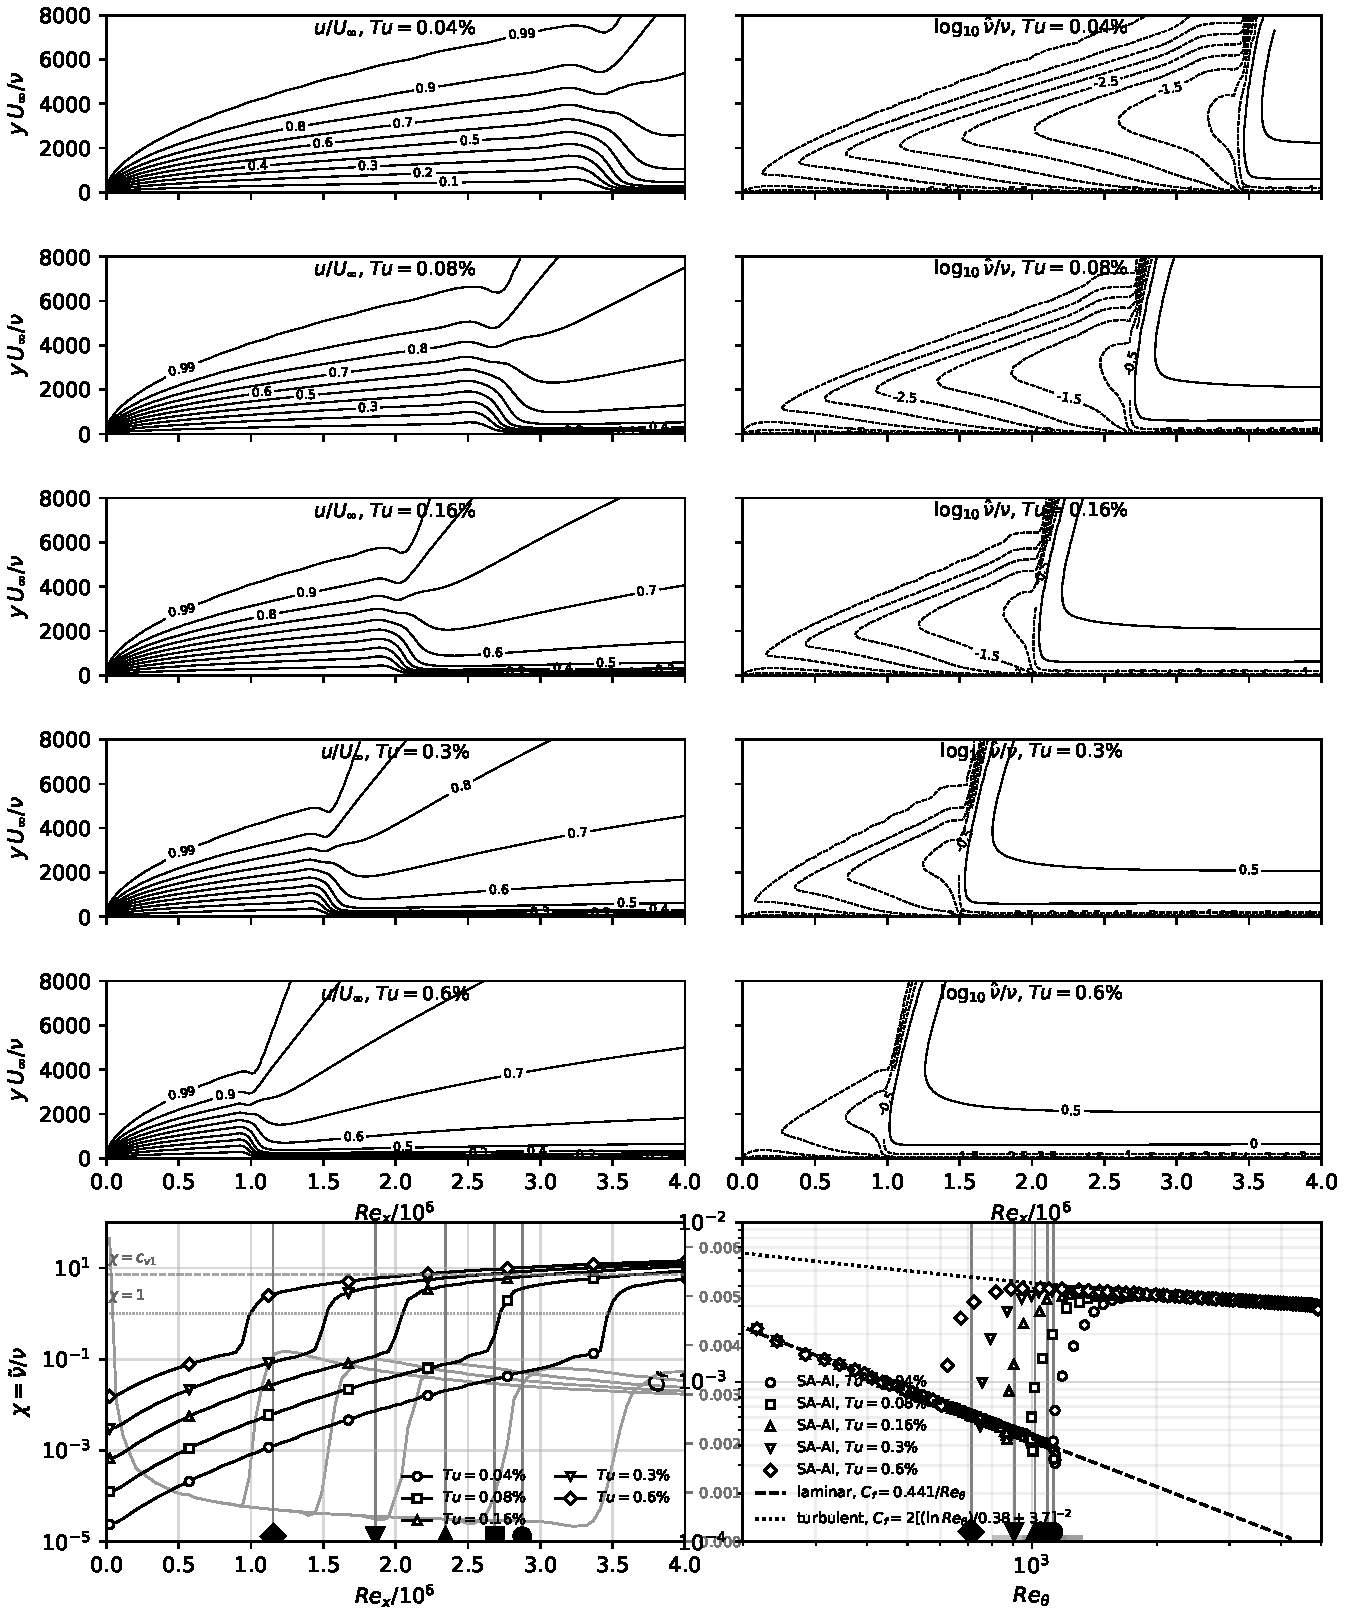
\includegraphics[width=0.90\textwidth]{flat_plate_batch_flow360.pdf}
  \caption{Freestream-turbulence sweep on the flat plate at five levels in the
  natural-transition range $Tu\!=\!0.04$--$0.60\%$ (rows). \emph{Left columns}:
  contours of $u/U_\infty$ and $\log_{10}\chi$ in the $(Re_x,Re_y)$ plane
  ($Re_x\!=\!x\!\cdot\!10^6$). \emph{Bottom-left}: in-BL maximum
  $\chi\!=\!\tilde\nu/\nu$ vs $Re_x$, with horizontal references at $\chi\!=\!1$
  (onset of the $\sigma_t$ blend) and $\chi\!=\!c_{v1}\!=\!7.1$ (eddy-viscosity
  half-saturation). \emph{Bottom-right}: $C_f$ vs $Re_\theta$ with the laminar
  ($C_f\!=\!0.441/Re_\theta$, dashed) and turbulent
  ($C_f\!=\!2[(\ln Re_\theta)/0.38+3.7]^{-2}$, dotted) correlations. Both
  bottom panels use black curves with one symbol per $Tu$ (legend); the
  bottom-left panel overlays $C_f$ (gray, right axis) on the $\chi$
  trajectories, locating each case's $C_f$ rise between its $\chi\!=\!1$
  and $\chi\!=\!c_{v1}$ crossings; solid-gray
  verticals and filled bottom-edge symbols mark the Abu-Ghannam \&
  Shaw~\cite{abu_ghannam_shaw_1980} transition-onset reference, and the
  bottom-right adds the digitized Schubauer--Skramstad
  Fig.~7 band (faint bars) for context. Thin steel-blue curves in both
  bottom panels: the independent cell-centered incompressible
  (OpenFOAM) implementation of the model on the same grid
  specification. With the receptivity taken from Mack's
  $e^N$ correlation, the model's half-saturation ($\chi\!=\!c_{v1}$)
  onset brackets AGS within
  $10\%$ across the range---late at the lowest $Tu$, early at the
  higher levels---while the $\chi\!=\!1$ blend-onset reading drifts
  early as the seed approaches unity (markers placed via the laminar
  $Re_\theta$--$Re_x$
  relation; the quoted residuals use the integrated $Re_\theta$ of the
  text); the
  $C_f$ follows the laminar branch then recovers the turbulent correlation
  (baseline SA, with no laminar branch, does not produce this).}
  \label{fig:flatplate_batch}
\end{figure}

\label{sec:calib_tu}%
A higher freestream turbulence intensity is a larger seed
$\chi_\infty$ and thus fewer $e$-folds to the handover, moving transition
upstream: a case seeded with $\chi_\infty$ reaches the handover where
its envelope crosses
$N_\mathrm{crit}\!=\!\ln(c_{v1}/\chi_\infty)$---the half-saturation
threshold $\chi\!=\!c_{v1}$ at which the eddy viscosity engages. We map
the turbulence intensity to the seed
by
\begin{equation}
  N_\mathrm{crit}(Tu) = -8.43 - 2.4\,\ln(Tu_{\mathrm{frac}}),
  \qquad
  \chi_\infty = c_{v1}\,e^{-N_\mathrm{crit}},
  \label{eq:tumap}
\end{equation}
with $Tu_{\mathrm{frac}}$ the rms turbulence intensity as a fraction. This is
Mack's~\cite{mack_1977, nasa_tmr} $e^N$ critical-$N$-factor correlation. The
correspondence is not exact: $e^N$ methods
declare transition at a sharp $N_\mathrm{crit}$, while the model's
threshold is smeared over the $\chi\!=\!1\!\to\!O(c_{v1})$
handover---several $e$-folds of the envelope.
Sensitivity to the seed is that of any $e^N$ method: one $e$-fold in
$\chi_\infty$ is one unit of $N_\mathrm{crit}$, which on the Blasius envelope
($dN/dRe_\theta\!\approx\!10^{-2}$) shifts onset by
$\Delta Re_\theta\!\approx\!100$.

In the solver the indicator triple is assembled from four local
vector-calculus objects and their invariant pairings alone: the
velocity $\mathbf u$ (taken relative to the nearest wall point, which
makes the triple Galilean invariant; for the static walls of this
paper, the absolute velocity), the vorticity $\boldsymbol\omega$, the
wall-distance vector $\mathbf d = d\,\nabla d$, and the curvature
vector
$\boldsymbol\ell = \tfrac12(\mathbf d\!\cdot\!\mathbf d)\,
\nabla^2\mathbf u$, where the divergence-free identity
$\nabla^2\mathbf u=-\nabla\times\boldsymbol\omega$ supplies the
second derivative; the onset gate's
$Re_\Omega\!=\!d^2|\boldsymbol\omega|/\nu$ completes the set. The
three-dimensional realization---its division-free Gram form,
Eq.~\eqref{eq:gram}, how the magnitude-based components realize the
signed algebra of Sec.~\ref{sec:model} exactly on all but a thin
mixed-sign layer of reversed profiles, and the two further pairings
the same four vectors admit---is stated in Appendix~E. Because the
rate depends on the frozen mean flow and never on $\tilde\nu$, the
production's $\tilde\nu$-derivative is analytic---the handover
derivative is its only stiff piece---and it is treated implicitly with
the same clipping as the baseline SA production.

Figure~\ref{fig:flatplate_batch} computes the model on the flat plate at five
freestream-turbulence levels spanning the natural-transition
range, $Tu\!=\!0.04\%,\,0.08\%,\,0.16\%,\,0.30\%,\,0.60\%$. The plate is
resolved by a structured $320\!\times\!80$ grid (streamwise $\times$
wall-normal). In units of the reference length (unit Reynolds
number $10^6$), the domain spans $0\!\le\!x\!\le\!6$
($Re_x\!\le\!6\!\times\!10^6$) streamwise and $0.5$ in the wall-normal direction;
the streamwise spacing is clustered at the leading edge (from
$\Delta x\!\approx\!8\!\times\!10^{-4}$, coarsening toward the outflow) and the
wall-normal spacing grows geometrically at ratio $1.12$ from a first-cell height
of $\approx\!7\!\times\!10^{-6}$ ($y^+\!\lesssim\!0.3$), resolving the laminar and
transitional boundary layer. The boundary conditions are no-slip on the plate, a
characteristic freestream on the far boundary, and slip walls on the two span
planes (quasi-2D); the freestream Mach number is $0.1$. An independent
cell-centered, pressure-based incompressible implementation of the
model, run on this same grid specification, reproduces the onset
crossings quoted below within $5\%$ in $Re_\theta$ uniformly across
the sweep, so neither the grid nor the discretization carries the
result. We compare the
resulting transition onset to the Abu-Ghannam \&
Shaw zero-pressure-gradient
correlation~\cite{abu_ghannam_shaw_1980}, $Re_\theta^\mathrm{tr}\!=\!163+\exp(6.91-Tu[\%])$ --- the
community-standard low-disturbance reference, itself a smooth fit through
flat-plate data including Schubauer \& Skramstad~\cite{schubauer_skramstad_1948}.
We use that correlation rather than Schubauer \& Skramstad's raw
Fig.~7 because that figure's low-$Tu$ \emph{plateau} (transition
fixed near $Re_x\!\approx\!2.8\!\times\!10^6$ below $Tu\!\approx\!0.08\%$) was
later shown by Wells~\cite{wells_1967} to be largely an artifact of
wind-tunnel acoustic noise rather than a true insensitivity to turbulence ---
a caveat Schubauer \& Skramstad themselves raise.

The Tu $\to\chi_\infty$ map of Eq.~\eqref{eq:tumap} sends each case to a single
freestream seed
($\chi_\infty\!\approx\!2.3\!\times\!10^{-4}$, $1.2\!\times\!10^{-3}$,
$6.3\!\times\!10^{-3}$, $2.9\!\times\!10^{-2}$, $1.5\!\times\!10^{-1}$ at the
five $Tu$; the delivered ambient matches these set values to four
digits at the boundary-layer edge at every station). Starting from this small laminar seed, $\tilde\nu$ remains inert
while the skin friction follows the laminar Blasius law (dashed); the
amplification \eqref{eq:pai} grows the disturbance through the unstable region
until $\chi$ reaches unity, after which $C_f$ rises toward the turbulent
log-law correlation (dotted). As $Tu$ rises the transition moves
forward.

The two bottom panels collect the in-BL maximum
$\chi$ (vs $Re_x$) and the resulting $C_f(Re_\theta)$. The
operational transition --- the $C_f$ rise --- runs between the $\chi\!=\!1$
crossing (the start of the $\sigma_t$ blend) and the
$\chi\!=\!c_{v1}\!=\!7.1$ crossing (the eddy-viscosity half-saturation
point): the bottom-left panel overlays $C_f$ (gray, right axis) on the
$\chi$ trajectories, and each case's rise starts at its $\chi\!=\!1$
crossing and levels off at its $\chi\!=\!c_{v1}$ crossing. Because the
modeled transition has finite extent, quoting a single onset number
against AGS requires choosing a crossing, and the comparison depends on
the choice; we state the convention and give both readings, with
$Re_\theta$ integrated from the computed profiles at the crossing
station (edge-normalized momentum thickness, integral cut at the
boundary-layer edge). At the
$\chi\!=\!1$ crossing---the start of the blend---the model reads
$+2\%$ late at the lowest disturbance level ($Tu\!=\!0.04\%$) and
drifts steadily early as the seed grows, $-8\%$ at $0.08\%$ to
$-27\%$ at $0.60\%$: the seed itself spans $15\times$ and approaches
unity, so the first crossing measures receptivity as much as growth
and is seed-level-sensitive by construction---which is why the quoted
onset convention is the other crossing. At the
$\chi\!=\!c_{v1}$ crossing---the half-saturation point, mid-way up
the $C_f$ rise, and the threshold the receptivity map itself is
anchored to ($\chi_\infty\!=\!c_{v1}e^{-N}$)---the model brackets the correlation within $10\%$
across the whole sweep: $+7\%$ late at $Tu\!=\!0.04\%$, $-2\%$ at
$0.08\%$, and $4$--$10\%$ early over $0.16$--$0.60\%$. The
onset residuals have different roots: the late bias at low $Tu$ is the
retained-drain footprint of the calibration (the marched Blasius
envelope runs $7\%$ past Drela's station by $N\!=\!9$,
Sec.~\ref{sec:calib_onset}, and the low-$Tu$ seeds hand over near that
depth), while the early bias at the higher levels traces to the
receptivity map \eqref{eq:tumap}, taken from
Mack's $e^N$ correlation without adjustment here; tightening either is
left to future work.

Strongly bypass-dominated
conditions ($Tu\!\gtrsim\!1\%$, e.g. the ERCOFTAC T3A and T3B test cases at
$Tu\!=\!3\%$ and $6\%$) lie outside this scope: at
$Tu\!=\!1\%$ the map
\eqref{eq:tumap} leaves only $N_\mathrm{crit}\!\approx\!2.6$---a seed already
within a few $e$-folds of handover---and by $Tu\!\approx\!3\%$ the seed
$\chi_\infty$ exceeds $c_{v1}$ outright, no longer a meaningful kinematic
parametrization of bypass transition. We therefore do not present T3A/T3B
comparisons.

\section{The NLF(1)-0416 airfoil at $Re\!=\!4\!\times\!10^6$}\label{sec:nlfval}

The natural-laminar-flow airfoil NLF(1)-0416 demands an $e^N$-style
instability tracker.
Figure~\ref{fig:nlfaft} tells most of the story: the computed
transition fronts across the incidence matrix, on every grid of both
mesh families, against the microphone measurements and the $e^N$
references. The model is evaluated at $Re\!=\!4\!\times\!10^6$, $M\!=\!0.1$,
$\chi_\infty\!=\!c_{v1}\,e^{-9}\!\approx\!8.76\!\times\!10^{-4}$
(the $N_\mathrm{crit}\!=\!9$ anchor, set through the map of Sec.~\ref{sec:calib_tu}; via Mack's
map, Eq.~\eqref{eq:tumap}, it corresponds to $Tu\!\approx\!0.07\%$, consistent
with the low-turbulence tunnel), across
$\alpha\!\in\!\{0^\circ, 4^\circ, 9^\circ,
15^\circ\}$, on a three-level isotropic refinement ladder of both mesh families
(unstructured cavity-mesher and structured O-grid, L0--L2, twenty-four
cases total). The finest grids extend the matrix to the
negative-incidence pair $\alpha\!=\!-8^\circ$ and $-4^\circ$
(Fig.~\ref{fig:nlfnegalpha}; wall-anchored contour sheets in
Appendix~A). The unstructured mesher uses a shared NLF contour (a natural cubic
spline in arc length through the published coordinates, resampled with
piecewise-cosine clustering) with
blunt-trailing-edge--aware spacing ($h_\mathrm{TE}$ scales with first-cell
height $h_0$ at every level; the TE ramp ratio $r_\mathrm{TE}$ decays from
$2.0$ at L0 to $1.25$ at L2 so that the local cell size at fixed chord-distance
from the TE also halves); the structured O-grid is generated with the same
contour by Construct2D~\cite{prosser_construct2d}. Every length scale---surface point count, $h_0$,
growth-ratio offset (the wall-normal growth ratio minus one), TE step, and TE
ramp---refines by a factor of two
per level. The two families also separate the solver classes: the
cavity meshes' anisotropic boundary-layer triangles are tractable for
the node-centered least-squares operators used here but defeat a
cell-centered compact-stencil discretization outright (the independent
cell-centered implementation of Sec.~\ref{sec:flatplate} diverges on
both the primal triangulation and its median dual, for standard SA as
much as for SA-AI), so the cross-solver replication carries the
structured family only.
Figures~\ref{fig:nlfmesh_str} and~\ref{fig:nlfmesh_cav} (appendix) show the
two mesh families at the leading and trailing edges across the three
refinement levels, and Table~\ref{tab:nlfmesh} lists their resolution
quantitatively.

\begin{figure}[tp]
  \centering
  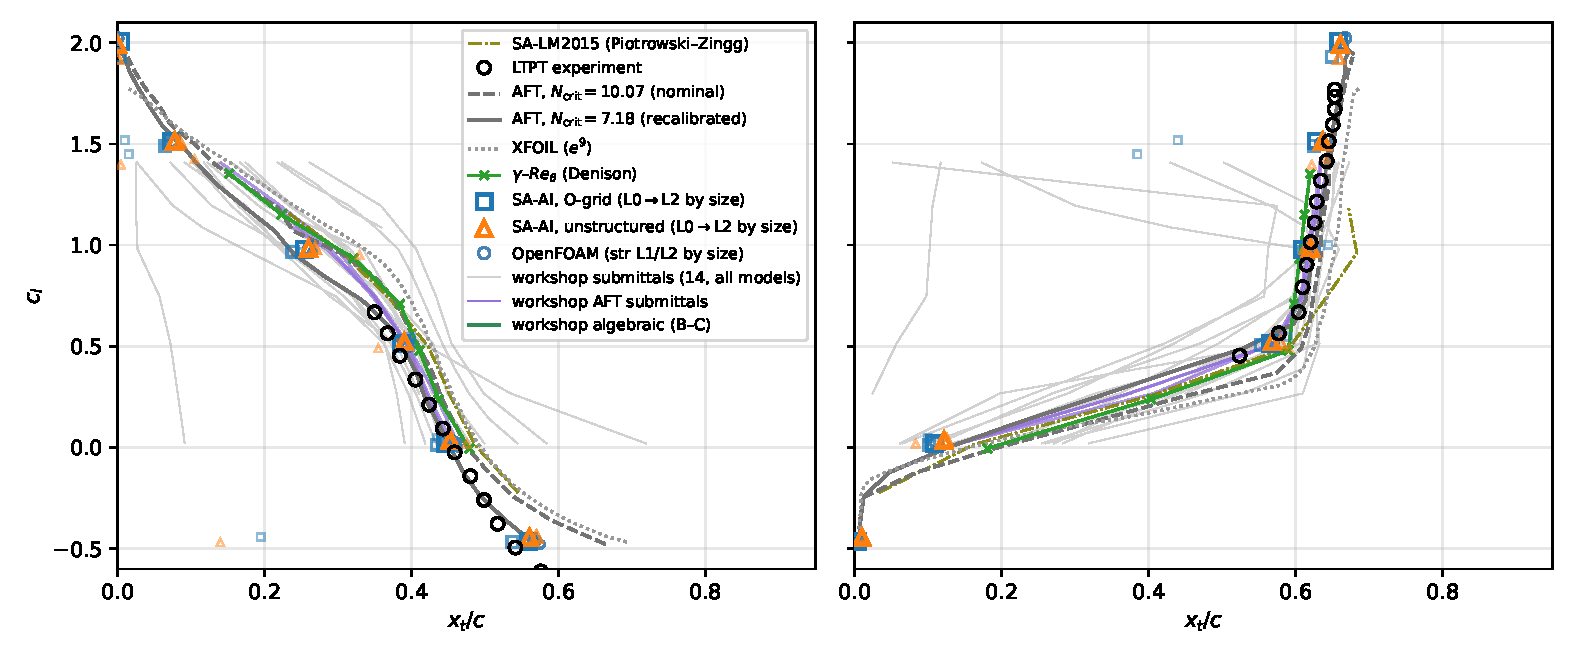
\includegraphics[width=\textwidth]{nlf_aft_transition.pdf}
  \caption{NLF(1)-0416 at $Re\!=\!4\!\times\!10^6$: transition location
  against lift coefficient, upper (left) and lower (right) surfaces.
  Circles: LTPT microphone measurements. Gray curves: the AFT model in
  OVERFLOW from Coder's dissertation~\cite{coder_thesis_2014} at its
  nominal $N_\mathrm{crit}\!=\!10.07$ (dashed) and after the
  source's recalibration to $N_\mathrm{crit}\!=\!7.18$ (solid), with
  its XFOIL reference (dotted); all extracted vector-exact from the
  source figures
  (\texttt{data/aft\_nlf0416\_digitized.json}). Thin underlaid
  curves: \emph{all fourteen submittals} to the First AIAA CFD
  Transition Modeling and Prediction Workshop's NLF(1)-0416 incidence
  sweep ($\alpha\!=\!-4^\circ$--$8^\circ$), digitized per
  submittal from the workshop-summary overlay~\cite{coder_tmpw_summary}
  (\texttt{data/workshop\_nlf\_submittals.json}, the only published
  collection of all participants) and placed on the lift axis through
  the computed structured-L2 lift curve (fourteen submittals,
  nineteen curves: two participants supplied second model variants and
  three line-only series carry no letter code); the AFT submittals are
  purple, the algebraic Bas--Cakmakcioglu submittal thin sea-green,
  all others light gray. Olive dash-dot: the SA-LM2015 fine-grid sweep of
  Piotrowski and Zingg~\cite{piotrowski_zingg_2021}, vector-digitized
  at its native $c_l$ ordinate. Dark-green crosses: the
  Langtry--Menter $\gamma$--$Re_\theta$ model in OVERFLOW (fine grid)
  from the transition-workshop exercise of
  Denison~\cite{denison_2021_overflow}, digitized from its Fig.~11
  (\texttt{data/lm\_nlf0416\_transition\_digitized.json}; the
  workshop condition is $M\!=\!0.2$, $Tu\!=\!0.15\%$---immaterial
  on transition-vs-$c_l$ axes). No published SA-BCM incidence
  \emph{sweep} exists at this condition; the one open SA-BCM result
  is a single-incidence ($\alpha\!=\!0^\circ$) mesh-adaptation
  study~\cite{tarsia_2025}. The isolated coarse-grid points at incidence are under-resolved-front artifacts (cf.\ the L0 discussion of Fig.~\ref{fig:nlfcflow}); the cavity-L1 $15^\circ$ lower front is the one unsettled case of the twenty-four, still drifting over $0.65$--$0.67\,c$ (the final value is plotted). Open squares/triangles:
  SA-AI on all six grids (L0--L2 by marker size, both families) at
  $\alpha\!=\!0^\circ,4^\circ,9^\circ,15^\circ$, plus the
  negative-incidence pair $\alpha\!=\!-8^\circ$ (well into the
  negative branch of the measured polar) and $-4^\circ$ (zero lift) on
  the finest grids,
  all at the paper-wide untuned seed. At $-8^\circ$ the drag sits $8$--$11$ counts below
  the measured polar at matched lift, the suction (lower) surface trips at
  $0.004$--$0.011\,c$, on the references' leading-edge trip ($e^9$:
  $0.015$--$0.018\,c$), and the pressure-side (upper) front
  converges at $0.559$--$0.561\,c$ (families agreeing to
  $0.002\,c$)---on the measured ${\approx}0.54\,c$, with the
  recalibrated AFT at $0.57$ and $e^9$ at $0.66\,c$.}
  \label{fig:nlfaft}
\end{figure}


\begin{table}[tp]
  \centering
  \small
  \caption{NLF(1)-0416 mesh ladder: size, wall-tangential and wall-normal
  resolution, and resulting $y^+$. Tangential spacing $\Delta s/c$ is measured on
  the upper surface; the wall-normal first-cell height $h_0$ and the cell size
  $0.5c$ off the wall are read from the center-span slice; the $y^+$ percentiles
  aggregate the four incidences ($\alpha\!=\!0^\circ,4^\circ,9^\circ,15^\circ$).
  The cavity meshes are all-triangular, the structured O-grids all-quadrilateral.}
  \label{tab:nlfmesh}
  \begin{tabular}{l cccccc}
    \toprule
    & \multicolumn{3}{c}{Unstructured cavity} & \multicolumn{3}{c}{Structured O-grid}\\
    \cmidrule(lr){2-4}\cmidrule(lr){5-7}
    & L0 & L1 & L2 & L0 & L1 & L2 \\
    \midrule
    Nodes    & 15{,}268 & 53{,}182 & 193{,}476 & 15{,}920 & 63{,}840 & 255{,}680 \\
    Elements & 29{,}855 & 105{,}481 & 385{,}665 & 15{,}721 & 63{,}441 & 254{,}881 \\
    \addlinespace
    $\Delta s/c$ @ LE ($\times10^{-3}$)      & 0.55 & 0.28 & 0.14 & 5.31 & 2.66 & 1.33 \\
    \quad @ $0.05c$                          & 5.73 & 2.85 & 1.42 & 10.5 & 5.23 & 2.61 \\
    \quad @ $0.25c$                          & 11.3 & 5.59 & 2.78 & 17.6 & 8.81 & 4.40 \\
    \quad @ $0.98c$                          & 6.57 & 6.22 & 4.10 & 2.74 & 1.38 & 0.69 \\
    \quad @ TE                               & 2.70 & 1.75 & 0.98 & 0.72 & 0.38 & 0.20 \\
    \addlinespace
    $h_0/c$ ($\times10^{-6}$)                & 12.6 & 5.6 & 2.6 & 7.0 & 3.5 & 1.8 \\
    cell @ $0.001c$ ($\times10^{-6}c$)       & 227 & 97 & 49 & 159 & 82 & 43 \\
    cell @ $0.5c$ ($\times10^{-2}c$)         & 8.45 & 4.41 & 2.21 & 2.19 & 1.07 & 0.52 \\
    \addlinespace
    $y^+$ (95th pct)                         & 2.99 & 2.10 & 1.22 & 1.90 & 0.92 & 0.46 \\
    $y^+$ (99th pct)                         & 4.26 & 3.12 & 2.05 & 2.53 & 1.39 & 0.70 \\
    \bottomrule
  \end{tabular}
\end{table}

The unstructured family is deliberately adversarial. Unlike the usual
``unstructured'' airfoil mesh---which grows a \emph{structured} layer of
wall-normal quadrilaterals or prisms through the boundary layer and Delaunay-triangulates
only the isotropic exterior---the cavity mesher applies the same
constrained-Delaunay triangulation everywhere, the boundary layer
included. There the metric is stretched by
$O(10^2\text{--}10^3)\!:\!1$, and the cavity point-insertion uses an anisotropic
distortion metric (with a skewness/normal-deviation objective) to promote
near-right-angled stretched triangles ($\sim\!90^\circ$-$90^\circ$-$0^\circ$)
over flat slivers ($\sim\!180^\circ$-$0^\circ$-$0^\circ$); but this is a
preference, not a guarantee, and the resolved boundary layer carries many
near-degenerate triangles (visible in Fig.~\ref{fig:nlfmesh_cav}, and reflected in
the elevated peak $y^+$ of the cavity grids in Table~\ref{tab:nlfmesh}). This directly
stresses the model, whose indicators ($Re_\Omega$ and the sphere coordinate
$\hat\Omega \hat I$, the latter carrying a \emph{second} velocity derivative in its
curvature term $\tfrac12 d^2\nabla^2u$) are all \emph{local} and gradient-based,
so sliver-induced errors in the computed gradients feed
straight into the amplification rate.
Figure~\ref{fig:nlfaft} shows the result: at L1 and L2 the cavity
markers land on the O-grid markers on every front.

This case also permits the paper's one direct comparison with the AFT
model, whose dissertation-stage validation ran the same airfoil at the
same Reynolds number in OVERFLOW~\cite{coder_thesis_2014}.
Figure~\ref{fig:nlfaft} overlays the two (the AFT, XFOIL, and
measurement curves are vector-exact extractions from the source's
figures). At its nominal tunnel calibration
($N_\mathrm{crit}\!=\!10.07$) the AFT fronts sit systematically
downstream of the microphone measurements, and the source closes the
gap by recalibrating to $N_\mathrm{crit}\!=\!7.18$
($Tu\!=\!0.15\%$), chosen from the transition-location discrepancy
itself. SA-AI's fronts, computed with the untuned $N\!=\!9$-class seed
($\chi_\infty\!=\!c_{v1}e^{-9}$), land
on the measurements where the recalibrated AFT lands, on both
surfaces and both mesh families. We do not read the untuned agreement
as a ranking, because it may be partly compensatory: the model's
laminar-to-turbulent handover is least decisive at low $Re_\theta$
(Sec.~\ref{sec:epphandover}), the $c_{v1}$-based $N_\mathrm{crit}$
convention was anchored on flat-plate transition at lower $Re_\theta$
than these fronts, and at the NLF's higher-$Re_\theta$ fronts the
same convention is effectively sharper---while AFT's recalibrated
freestream may equally be read as absorbing the tunnel's true
disturbance level rather than as a per-case tuning.

\begin{figure}[tp]
  \centering
  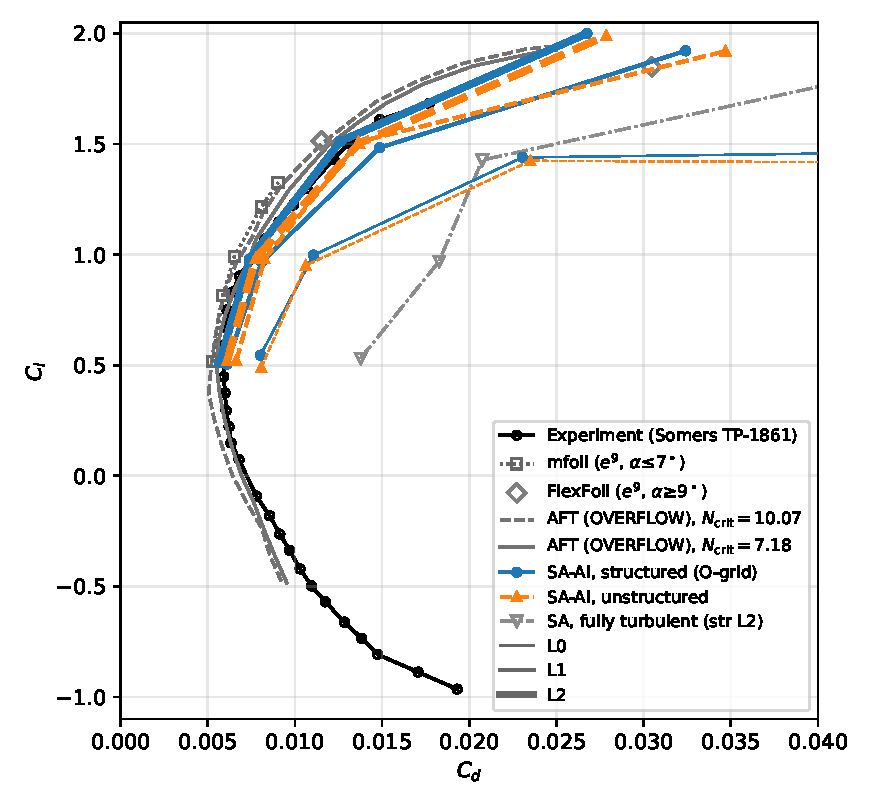
\includegraphics[width=0.62\textwidth]{nlf_polar_compare.pdf}
  \caption{Drag polar of the NLF(1)-0416 at $Re\!=\!4\!\times\!10^6$: the present
  SA-AI prediction (structured O-grid and unstructured meshes, all three
  refinement levels) at $\alpha\!\in\!\{0^\circ,4^\circ,9^\circ,15^\circ\}$ (all
  six grids), extended on the finest grids through
  $\alpha\!=\!-4^\circ$ and $-8^\circ$ to $c_l\!\approx\!-0.46$,
  overlaid on the digitized experimental section characteristics (Somers, NASA
  TP-1861, Fig.~11d~\cite{somers_1981}) and the mfoil $e^9$ reference. Mesh family
  sets the color (blue = O-grid, orange = unstructured); refinement sets the line
  weight (L0 thin $\to$ L2 thick). The mfoil reference (gray squares) is shown
  where its coupled solve converges to an attached solution ($\alpha\!\le\!7^\circ$);
  at $\alpha\!=\!9^\circ$ and $15^\circ$, where mfoil fails, the $e^9$ reference is
  FlexFoil's (gray diamonds; FlexFoil is a separate implementation
  of XFOIL's viscous--inviscid $e^9$
  method~\cite{drela_xfoil_1989}, cross-checked against mfoil and
  XFOIL to $<\!1\%$ where all three converge). The two gray AFT (OVERFLOW) polars are digitized from the same
  dissertation source as Fig.~\ref{fig:nlfaft} (dashed:
  $N_\mathrm{crit}\!=\!10.07$; solid: the recalibrated $7.18$); they
  end mid-plot because the source figure's axis stops at
  $c_d\!=\!0.025$. Thin underlaid curves: the
  workshop submittals' polars, as in Fig.~\ref{fig:nlfaft}
  (AFT purple, Bas--Cakmakcioglu sea-green, others light gray; segments
  break where the source's marker identity is ambiguous). The gray dash-dot curve is
  fully turbulent SA ($\chi_\infty\!=\!3$, same solver, structured L2 grid):
  without the laminar run the drag sits $1.6$--$2.5\times$ above the
  SA-AI polar ($+144$/$+150\%$ in the bucket at $\alpha\!=\!0^\circ$/$4^\circ$,
  $+67$/$+74\%$ at $9^\circ$/$15^\circ$).}
  \label{fig:nlfpolar}
\end{figure}

Two entries in the polar (Fig.~\ref{fig:nlfpolar}) need
qualification. The $\alpha\!=\!15^\circ$ point lies beyond the measured
stall ($C_{l,\max}\!\approx\!1.68$ in the tunnel data), where the quasi-2D
computation does not capture stall and returns a higher
$C_l$ at elevated drag; and the coarse L0 mesh over-predicts drag at
$\alpha\!\ge\!9^\circ$ (under-resolved transition front). The absence of an
mfoil reference above $\alpha\!=\!7^\circ$ is a solver failure, not a
method-class limit: FlexFoil converges at the identical conditions
($C_l\!=\!1.51$ at $\alpha\!=\!9^\circ$, consistent with the present
RANS), as does XFOIL (its digitized $e^9$ curve in
Fig.~\ref{fig:nlfaft} spans these incidences). The fully turbulent SA
polar on the same structured L2 grid closes on SA-AI only as the laminar
run shrinks ($+144\%$ at $0^\circ$ narrowing to $+67$--$74\%$ at
$9^\circ$--$15^\circ$).

The airfoil surface distributions are presented as five-row figures
(Figs.~\ref{fig:nlfcflow}--\ref{fig:nlfcfhigh} here and
Figs.~\ref{fig:eppcflow}--\ref{fig:eppcfhigh} for the Eppler 387) with a
common layout: \emph{row 1} the wall-normal-probe maximum of $Re_\Omega$
(log, the onset gate); \emph{row 2} the wall-normal-probe maximum of the sphere
rate coordinate $\hat\Omega \hat I$ (Eq.~\eqref{eq:rate})---the amplifying inflectional
coordinate the kernel acts on, on a log axis spanning the amplifying
decades (suppressed and favorable stations, $\hat\Omega \hat I\!\le\!0$,
fall below the plotted range), with the rate
$a_{\max}\operatorname{clip}\langle \hat\Omega \hat I\rangle$; the field is
neighbor-smoothed (${\approx}0.5\%$ chord streamwise, $5\%$ of the
probe wall-normal) before the maximum is taken, because the
transported $\tilde\nu$ integrates production along streamlines, so
isolated single-point rate values---mesh noise on the unstructured
family---have no effect on the solution and a raw pointwise maximum
would over-report them; \emph{row 3} the in-BL maximum
$\chi\!=\!\max_y\tilde\nu/\nu$ on a log axis with the amplification factor $N$ from
mfoil~\cite{fidkowski_mfoil_2022}, a coupled viscous--inviscid $e^N$ panel solver,
on a linear right axis, the two linked by $N\!=\!\ln(\chi/\chi_\infty)$ so
one unit on the right equals one $e$-fold on the left (vertical dotted lines:
mfoil $x_\mathrm{tr}$); \emph{row 4} $-C_p$; \emph{row 5} $C_f$.

\begin{figure}[tp]
  \centering
  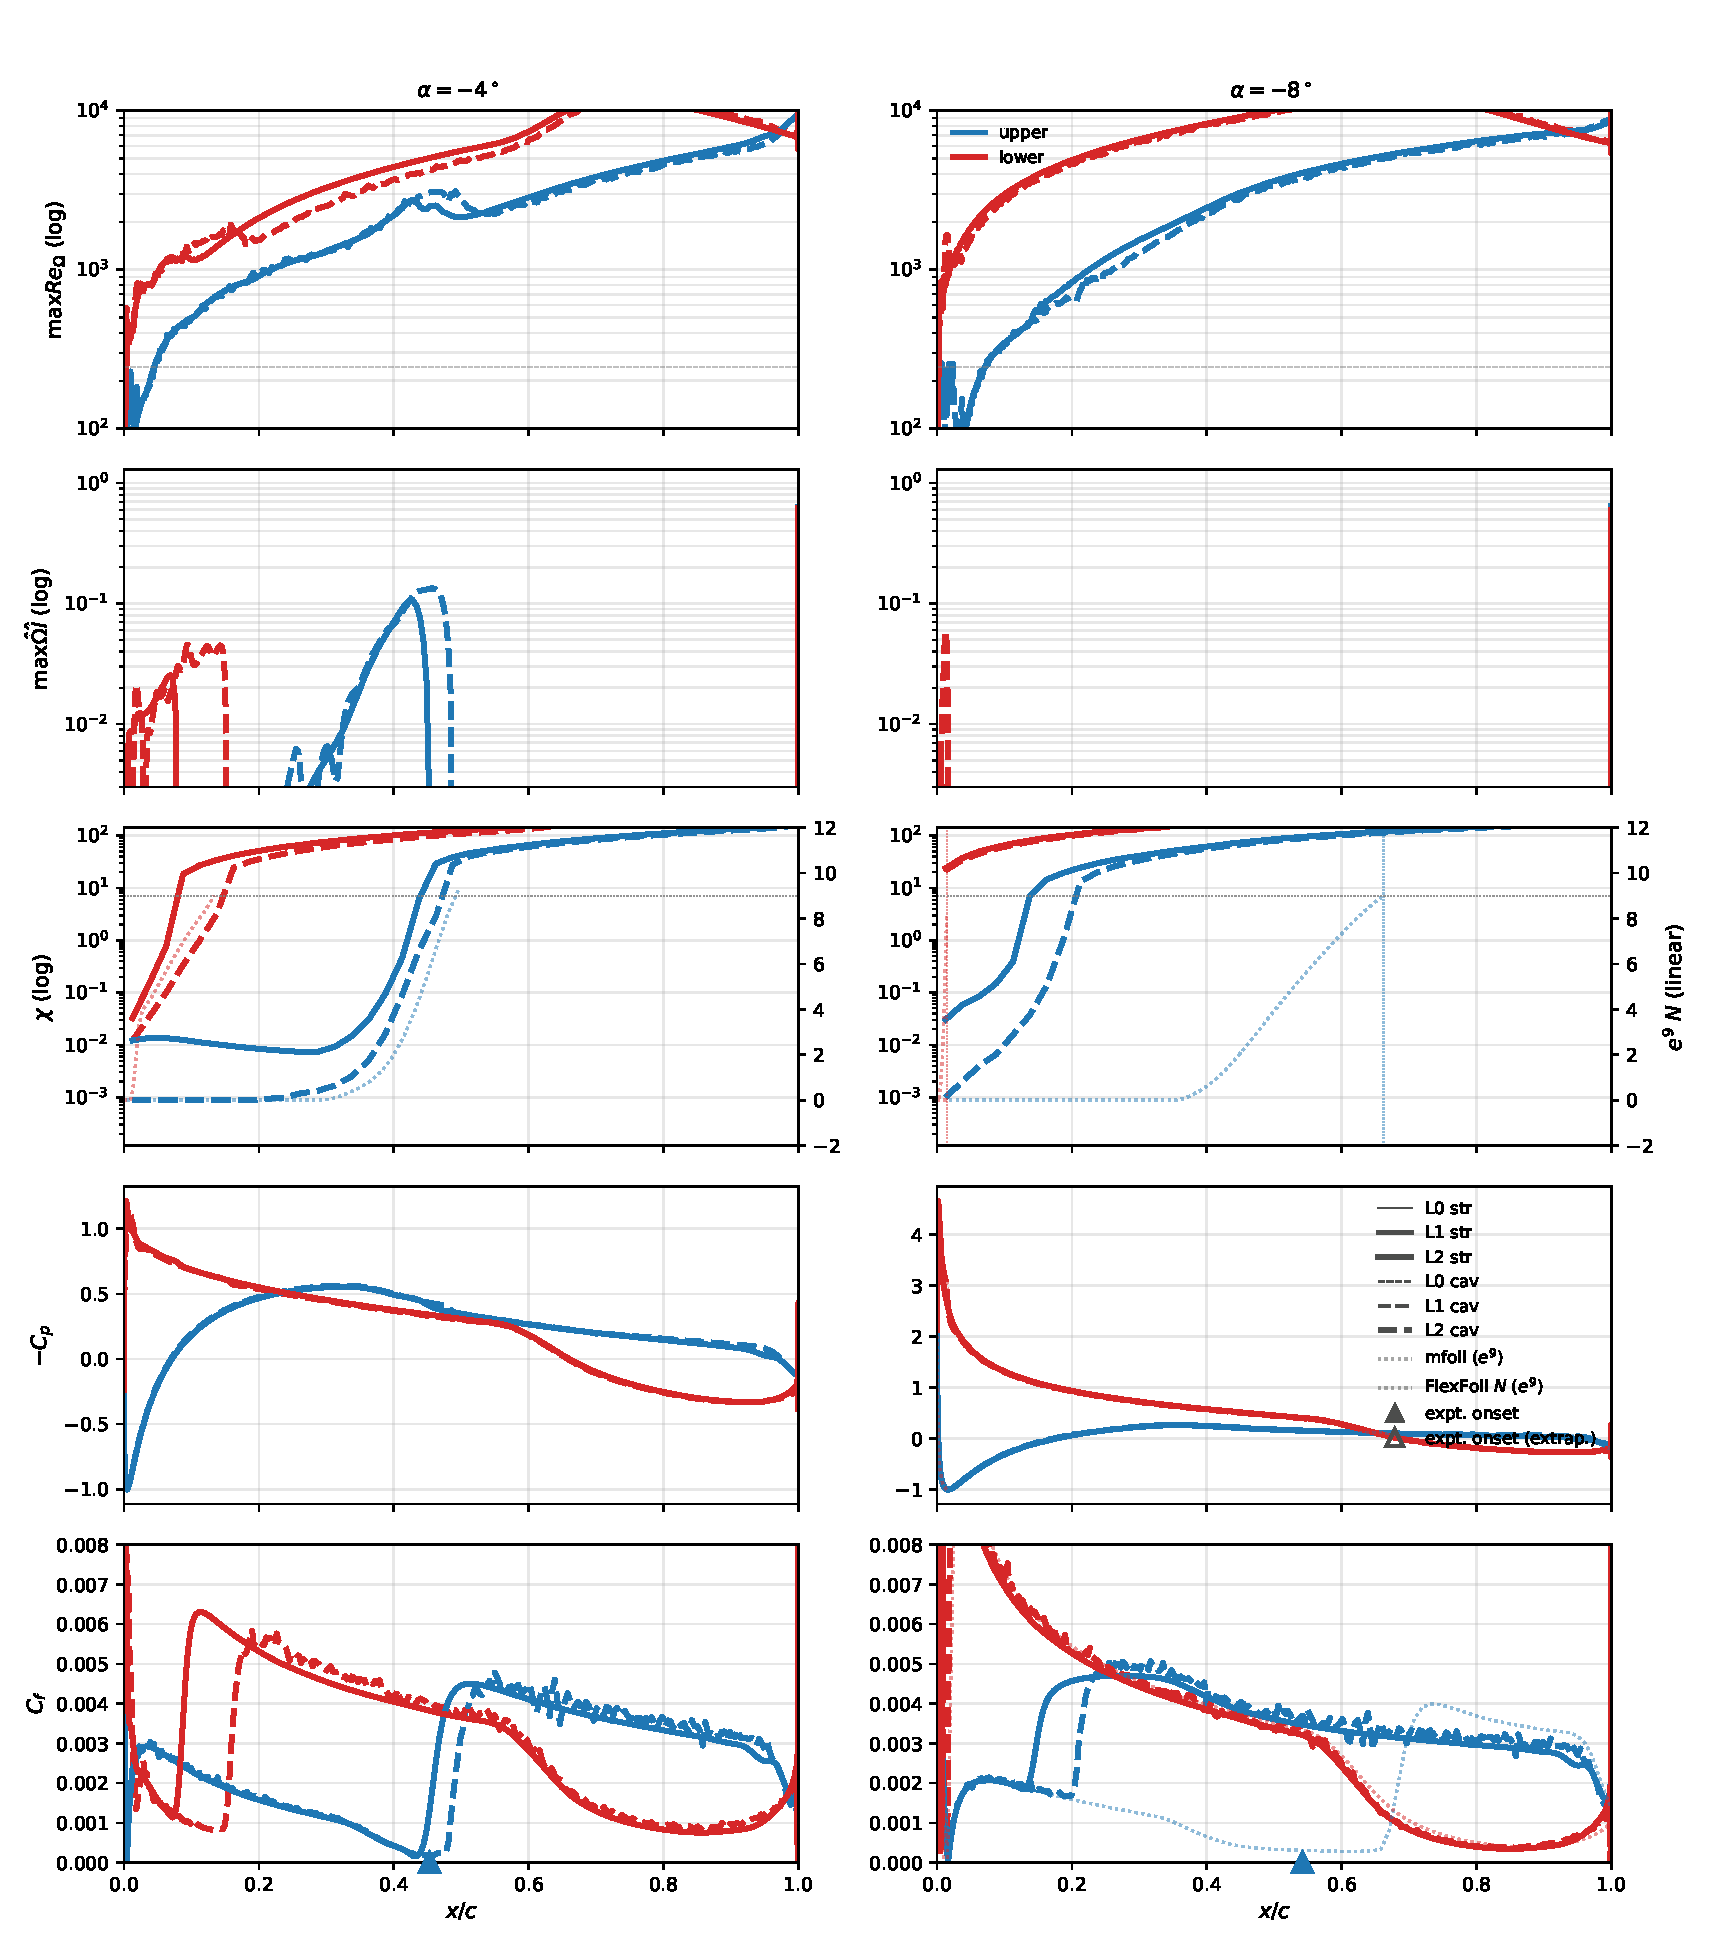
\includegraphics[width=0.96\textwidth]{nlf_cf_negalpha.pdf}
  \caption{NLF(1)-0416 at the negative-incidence pair
  $\alpha\!=\!-8^\circ$ (left, well into the negative branch of the
  measured polar) and $-4^\circ$ (right, zero lift), finest (L2)
  grids of both mesh families, with the five-row suite and line
  conventions described in the text (rows: probe-max
  $Re_\Omega$, probe-max $\hat\Omega \hat I$, near-wall $\max\chi$ with the
  $e^9$ $N$ envelope, $-C_p$, signed $C_f$; upper surface blue, lower
  red). The $e^9$ overlay is mfoil at $-8^\circ$ and FlexFoil at
  $-4^\circ$, where mfoil's coupled solve does not converge; filled
  triangle: measured onset at the computed lift. At $-4^\circ$ both
  fronts land on the references. At $-8^\circ$ the suction (lower)
  surface trips at $0.004$--$0.011\,c$, on the $e^9$ leading-edge
  trip, while the pressure-side (upper) front settles at
  $0.559$--$0.561\,c$, on the measured ${\approx}0.54\,c$ ($e^9$:
  $0.66\,c$).
  The wall-anchored contour sheets appear in Appendix~A
  (Figs.~\ref{fig:sheet_nlf0416_negalpha_upper}--\ref{fig:sheet_nlf0416_negalpha_lower}).}
  \label{fig:nlfnegalpha}
\end{figure}

\begin{figure}[tp]
  \centering
  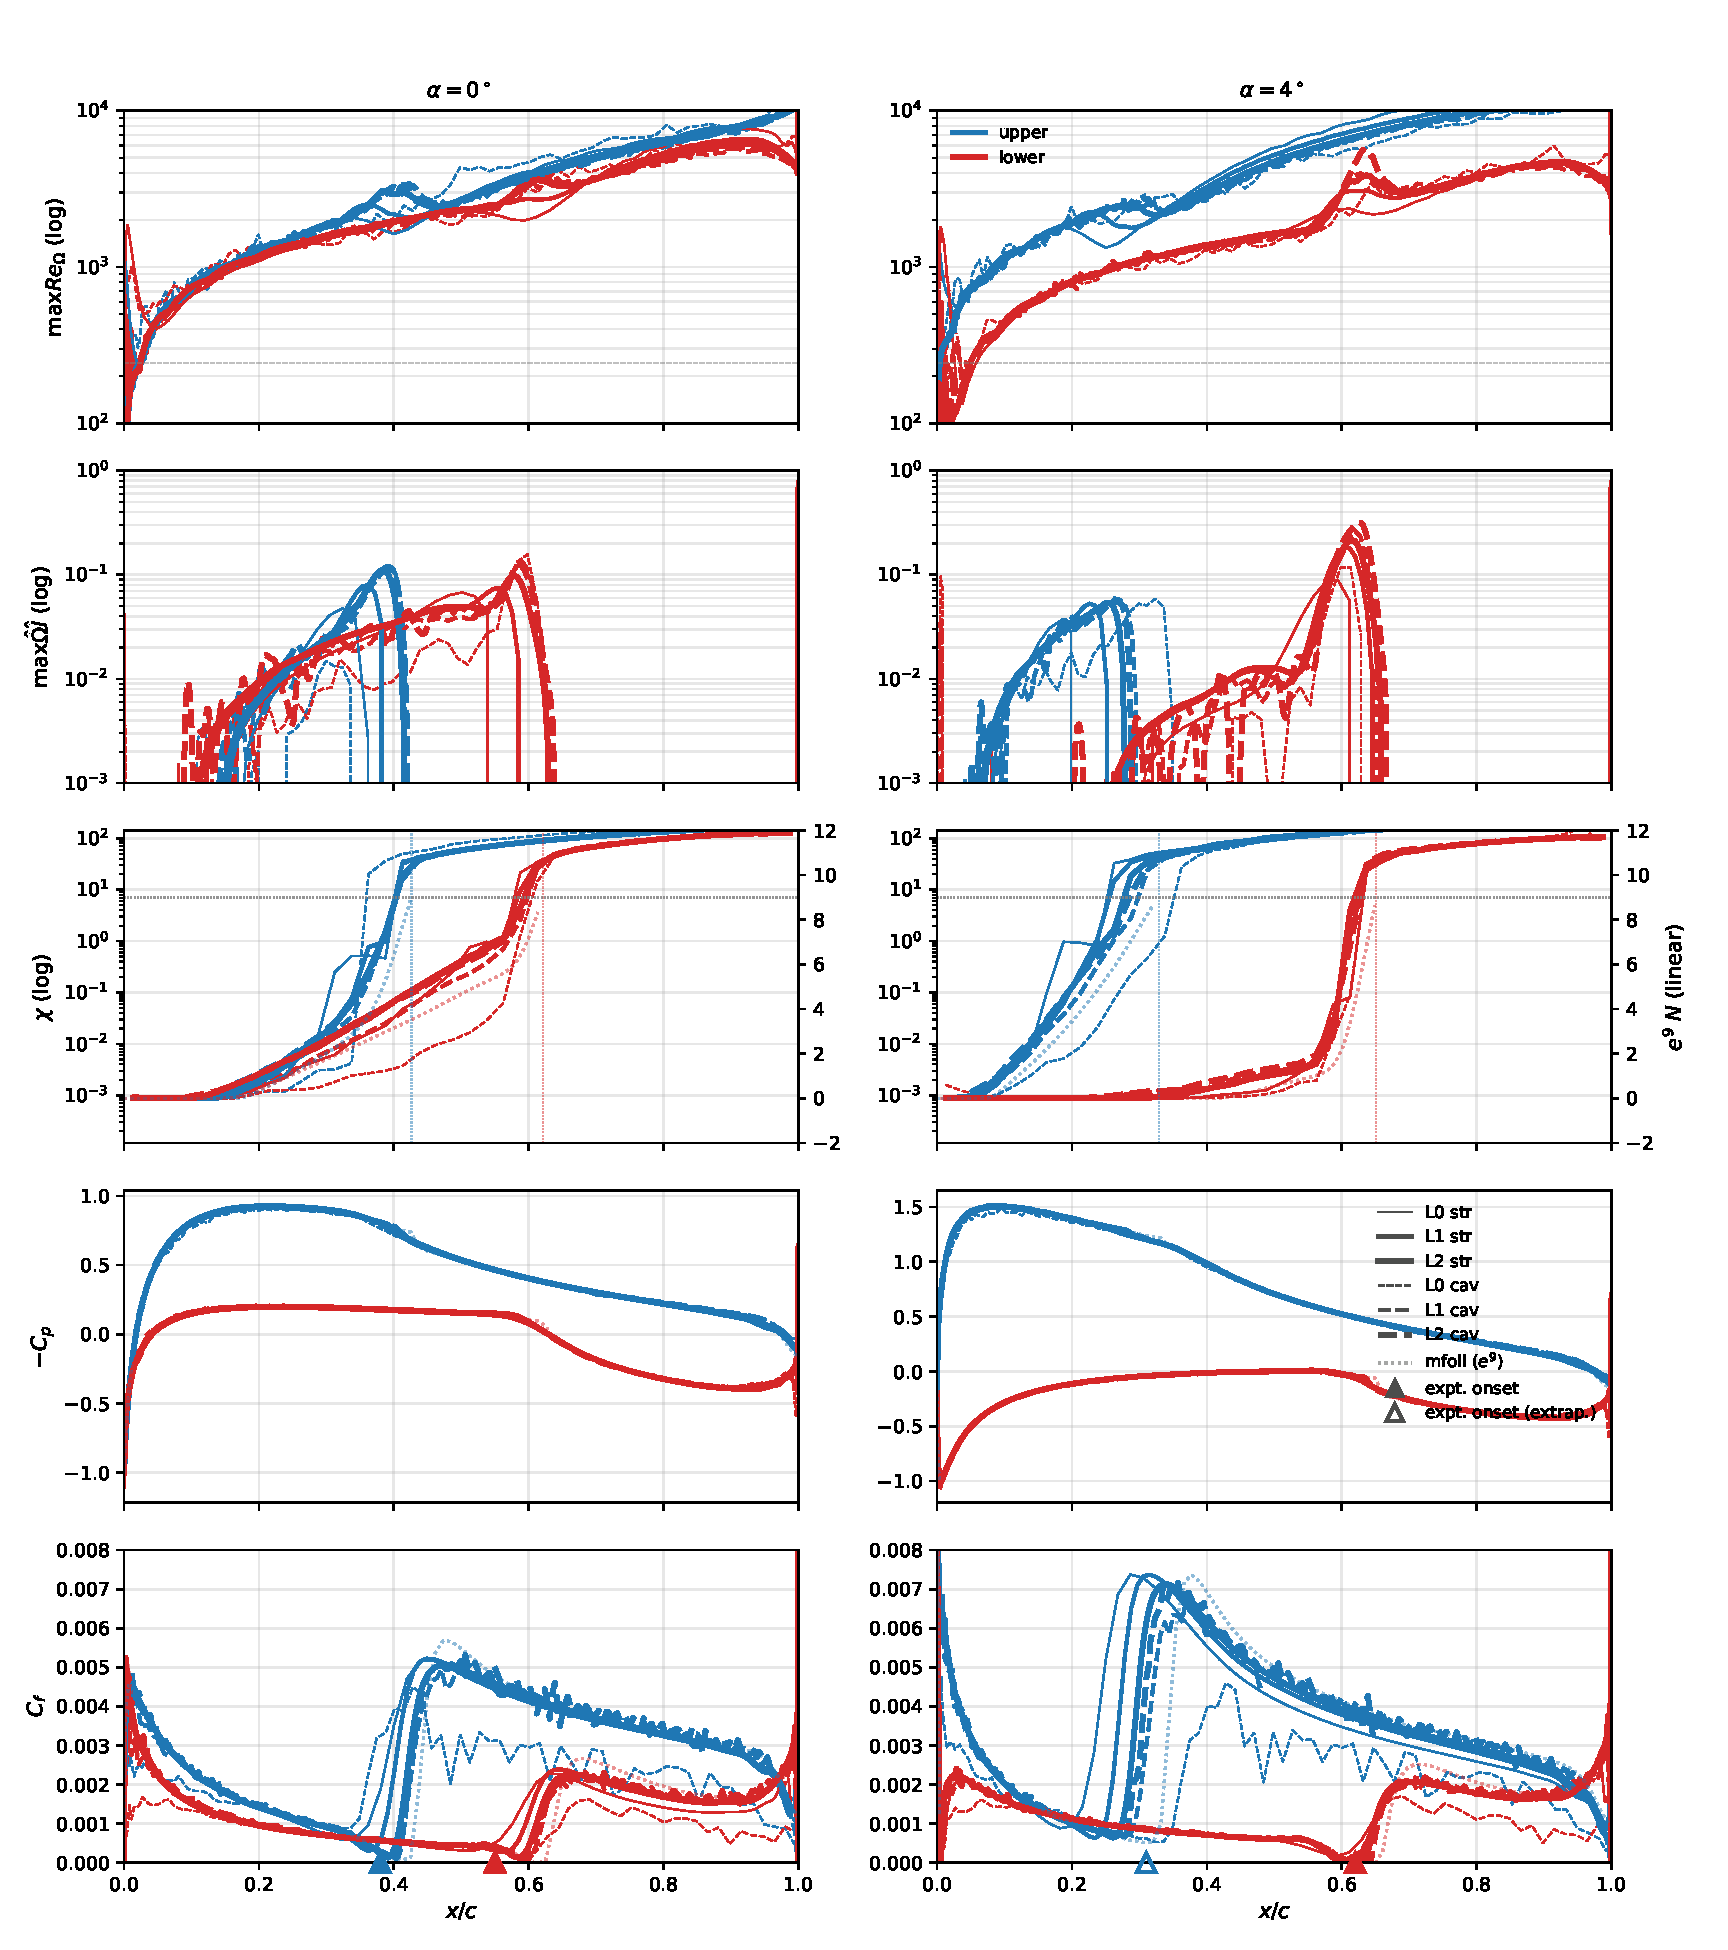
\includegraphics[width=0.99\textwidth]{nlf_cf_lowalpha.pdf}
  \caption{NLF(1)-0416 surface distributions at $\alpha\!\in\!\{0^\circ,4^\circ\}$,
  $Re\!=\!4\!\times\!10^6$, $\chi_\infty\!=\!8.76\!\times\!10^{-4}$. Five-row
  layout and line conventions as described in the text (row~1 $\max Re_\Omega$,
  row~2 $\max \hat\Omega \hat I$, row~3 $\chi$
  with mfoil $N$, row~4 $-C_p$,
  row~5 $C_f$; upper blue / lower red, O-grid solid / cavity dashed,
  L0--L2 by thickness, mfoil $e^9$ dotted; triangles on the $C_f$ row mark
  the measured onsets---Somers's transition orifices
  (Fig.~9d of Ref.~\cite{somers_1981}) read at the
  computed section $c_l$---open where extrapolated beyond the recorded
  data). At $\alpha\!=\!0^\circ$ both
  surfaces run laminar past a third of the chord (upper
  $x/c\!\approx\!0.38$--$0.39$, lower $0.56$--$0.57$), recovering the
  low-drag
  bucket; at $\alpha\!=\!4^\circ$ the upper-surface transition has marched
  forward to $x/c\!\approx\!0.25$ while the lower stays near design. The
  stall-and-dip of the L0 $\chi$ curves over the last two cells before
  transition is a purely numerical artifact of the under-resolved
  laminar--turbulent jump ($\sigma_t$ is not involved: $\chi\!<\!1$ there).
  Compressed into less than one cell, the jump's discretization error
  reaches two to three cells upstream and distorts the velocity profile;
  the rate coordinate $\hat\Omega \hat I$ at the amplifying point collapses toward zero,
  stalling the amplification. On L1 and L2, $\hat\Omega \hat I$ holds steady through the same station,
  $\chi$ rises monotonically, and the small L0 onset shift converges out.}
  \label{fig:nlfcflow}
\end{figure}

\begin{figure}[tp]
  \centering
  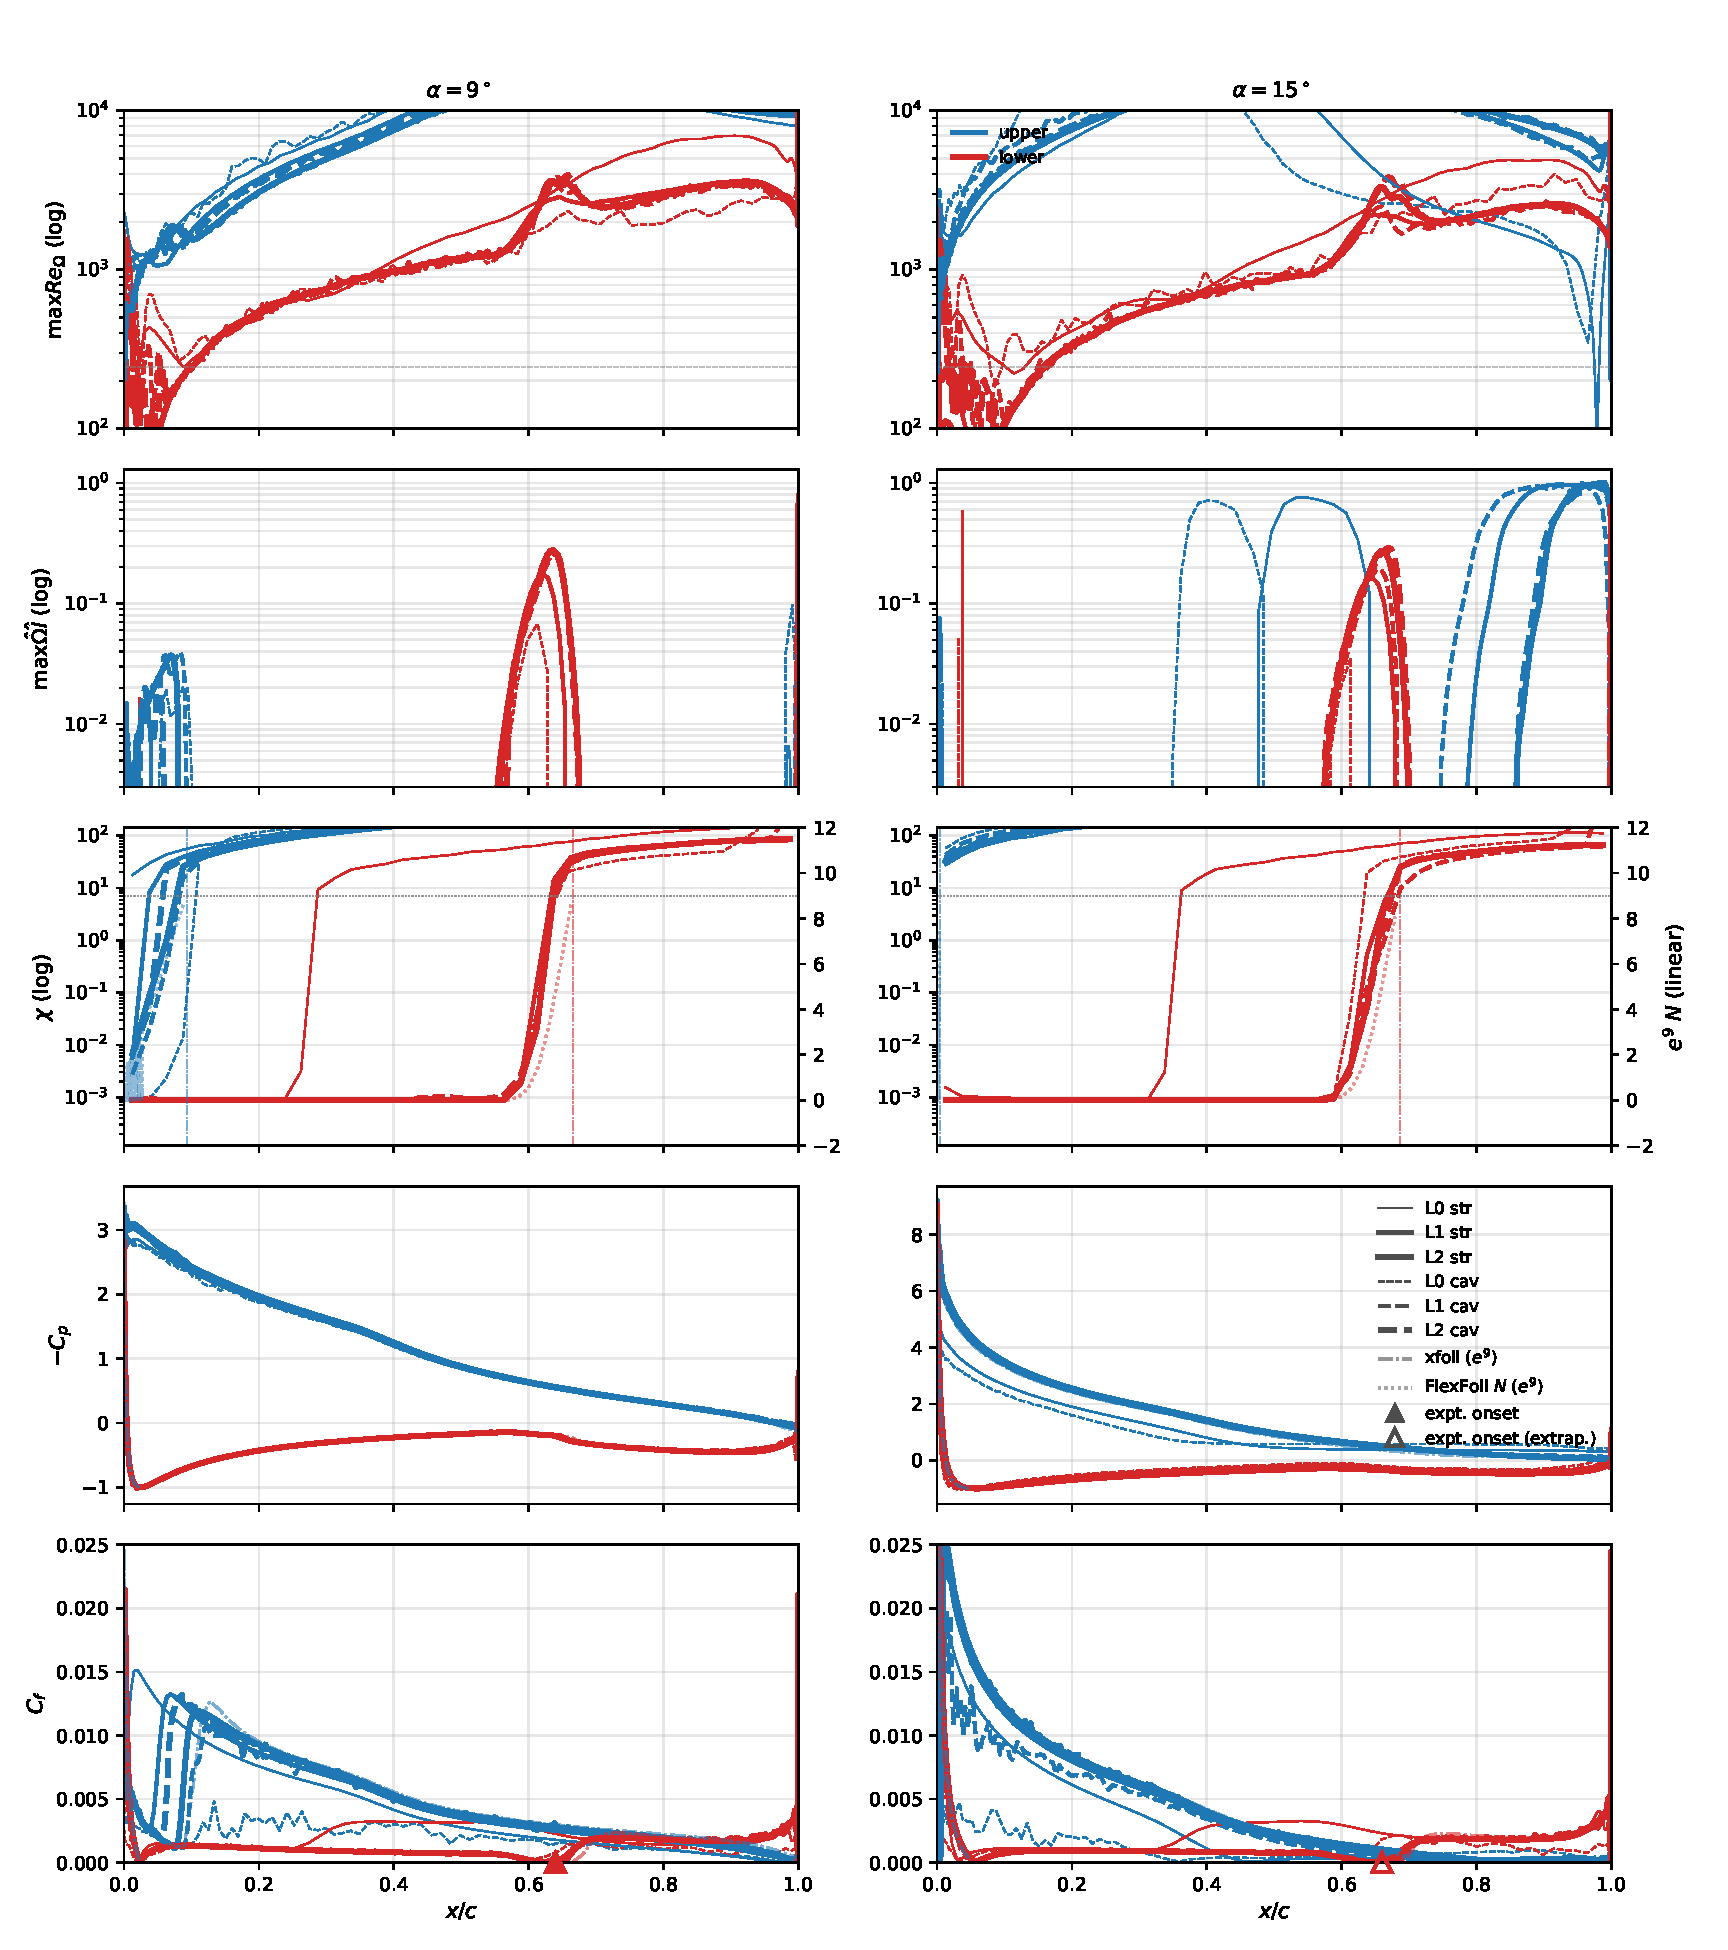
\includegraphics[width=0.99\textwidth]{nlf_cf_highalpha.pdf}
  \caption{As Fig.~\ref{fig:nlfcflow}, at $\alpha\!\in\!\{9^\circ,15^\circ\}$.
  The upper-surface transition has marched to $x/c\!\lesssim\!0.05$ at
  $\alpha\!=\!9^\circ$ and is at the LE by $\alpha\!=\!15^\circ$, while the
  lower transition remains aft of mid-chord. mfoil does not converge at
  $\alpha\!=\!9^\circ$ and stalls at $15^\circ$, so the $e^9$ overlay
  (dash-dot: $C_p$, $C_f$---converted from XFOIL's edge-normalized
  dump to the freestream convention, $\times u_e^2$---and transition
  location) is XFOIL's~\cite{drela_xfoil_1989}, and the continuous
  amplification envelope $N(x)$ (row~3, dotted) is FlexFoil's---a
  separately written implementation of the same closure set whose
  envelopes match mfoil's where both exist
  (Sec.~\ref{sec:eppresweep}). The L0 unstructured under-resolves
  the LE suction peak by $\sim\!1$ in $-C_p$ at $\alpha\!=\!15^\circ$ (thin
  dashed blue); L1/L2 collapse on both grids. The high-incidence cases test
  the amplification model under a strong adverse gradient:
  $\chi$ rises through $c_{v1}$ within the first few percent of chord on the
  upper surface, but the model still resolves a finite laminar dip and the
  laminar/turbulent handover stays at one chordwise location across the
  refinement series.}
  \label{fig:nlfcfhigh}
\end{figure}


Because a favorable gradient keeps the profile's curvature single-signed
($\hat\Omega \hat I\!\to\!0$), the model holds the favorable rooftop laminar with no
pressure-gradient parameter anywhere: amplification is confined to the
recovery stretch, where the profile turns inflectional ($\hat\Omega \hat I\!>\!0$)
and the fronts are set.

\section{The Eppler 387 low-Reynolds-number airfoil}\label{sec:eppval}

The Eppler 387 tests the low-Reynolds-number,
bubble-dominated regime. The McGhee, Walker, and Millard experiment in
the NASA Langley Low-Turbulence Pressure Tunnel \cite{mcghee_1988} tested this
airfoil from $Re\!=\!6\!\times\!10^4$ to $4.6\!\times\!10^5$ at tunnel
turbulence levels between $0.06\%$ and $0.18\%$; the data are the canonical
reference for low-$Re$ transition modeling and supply the comparison condition
used by Coder and Maughmer's AFT-2014, Coder's AFT-2017, the Langtry--Menter
$\gamma$--$Re_\theta$ benchmark, and the Bas--{\c C}akmak{\c c}{\i}o{\u g}lu
algebraic SA-BCM variant
\cite{coder_maughmer_2014, halila_2022, langtry_menter_2009, cakmakcioglu_2018}.
At these conditions the upper surface carries a long laminar-separation bubble
(LSB) that controls the section drag: laminar separation at the shoulder of the
suction peak, an inflectional shear layer in which the rate kernel must
accelerate amplification, turbulent reattachment, and a short turbulent wedge
to the trailing edge.

The model is evaluated at the de-facto benchmark condition of the
transition-modeling literature: $Re\!=\!2\!\times\!10^5$, $M\!=\!0.1$, across
$\alpha\!\in\!\{0^\circ,2^\circ,5^\circ,7^\circ\}$, with the freestream seed at
the same $N_\mathrm{crit}\!=\!9$ anchor as the NLF,
$\chi_\infty\!=\!8.76\!\times\!10^{-4}$ (the LTPT-class value). Three
refinement levels on two independently-generated mesh families
(unstructured cavity, structured O-grid) give twenty-four cases. The
finest (L2) pair extends the matrix with six further incidences,
$\alpha\!=\!-2^\circ$, $1^\circ$, $3^\circ$, $4^\circ$, $6^\circ$, and
$8.5^\circ$ (twelve additional solutions), spanning the measured polar
end to end.

Mesh generation reuses the NLF recipe verbatim. The 56-point Eppler 387
contour is read from the NASA TM 4062 Table I (design coordinates with the
trailing edge thickened from $0$ to $0.01\,\mathrm{in}$ blended at
$x/c\!=\!0.95$; $z_\mathrm{TE}\!=\!\pm0.000833\,c$, half the NLF
blunt-thickness), interpolated by the same natural cubic spline in
arc length as the NLF contour, resampled at $N\!\in\!\{200,400,800\}$
points with piecewise-cosine clustering at the LE and TE, and fed to both the
in-house unstructured cavity mesher and Construct2D; the far-field is fixed at
$100\,c$. The resulting grids range
from $1.5\!\times\!10^4$ nodes at L0 to $2.6\!\times\!10^5$ at L2.
Figures~\ref{fig:eppmesh_str} and~\ref{fig:eppmesh_cav} (appendix) show the
two mesh families at the leading and trailing edges across the three levels,
and Table~\ref{tab:eppmesh} lists their resolution quantitatively.

\begin{figure}[tp]
  \centering
  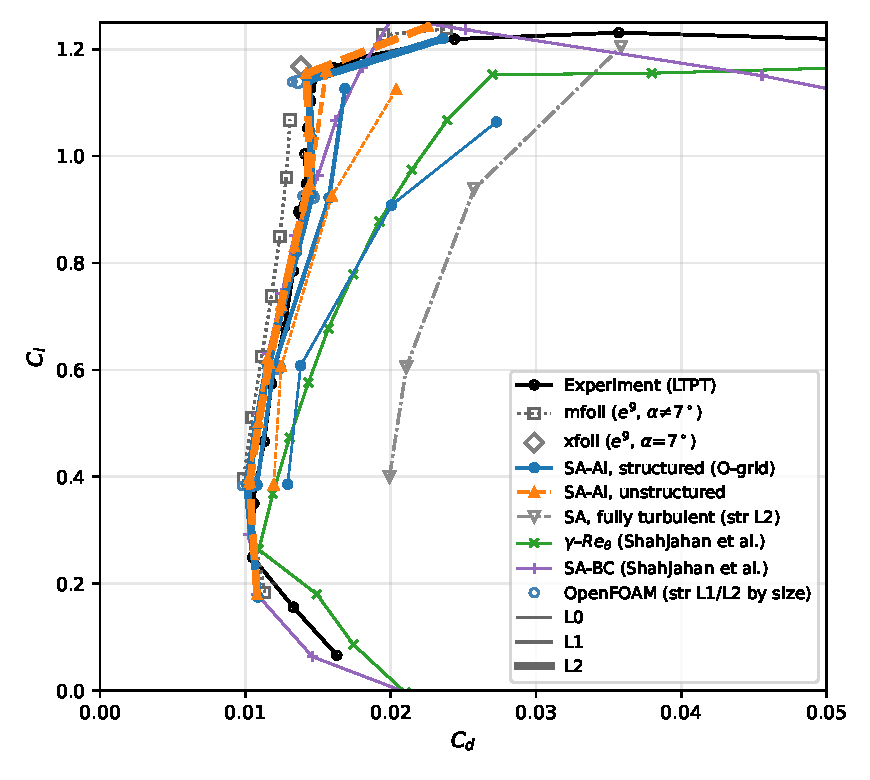
\includegraphics[width=0.62\textwidth]{eppler_polar_compare.pdf}
  \caption{Drag polar of the Eppler 387 at $Re\!=\!2\!\times\!10^5$: the present
  SA-AI prediction (all six grids at
  $\alpha\!\in\!\{0^\circ,2^\circ,5^\circ,7^\circ\}$; the finest
  L2 pair extended over $\alpha\!=\!-2^\circ$--$8.5^\circ$ with the
  six additional computed incidences) overlaid on the digitized
  experimental section characteristics from the Langley Low-Turbulence Pressure
  Tunnel (McGhee et al., NASA TM-4062, App.~B, $R\!=\!2\!\times\!10^5$) and the
  mfoil $e^9$ reference, spanning the same extended incidence
  range (XFOIL fills $\alpha\!=\!7^\circ$, where mfoil's coupled solve
  fails). The computed points track the low-drag laminar bucket;
  the two mesh families agree to within
  $\Delta C_d\!\le\!2.4\times10^{-4}$ across $\alpha\!=\!-2^\circ$--$7^\circ$
  and to $1.0\!\times\!10^{-3}$ at the unsteady $8.5^\circ$ point.
  The gray dash-dot curve is fully turbulent SA ($\chi_\infty\!=\!3$, same
  solver, structured L2 grid), $77$--$97\%$ above the SA-AI drag in the
  bucket and $+151\%$ at $\alpha\!=\!7^\circ$. The green and purple
  curves are the $\gamma$--$Re_\theta$ (Langtry--Menter, OpenFOAM) and
  SA-BC (SU2) transition models at the same condition and
  $Tu\!=\!0.1\%$, digitized vector-exact from
  Ref.~\cite{shahjahan_2024}
  (\texttt{data/lmbcm\_eppler387\_digitized.json}); the SA-BC
  intermittency correlation was calibrated in part on this
  airfoil~\cite{cakmakcioglu_2017}.}
  \label{fig:epppolar}
\end{figure}

On the finest grids the SA-AI polar (Fig.~\ref{fig:epppolar}) tracks the
measured low-drag bucket over $\alpha\!=\!0^\circ$--$7^\circ$
($c_l\!\approx\!0.38$--$1.15$) at matched lift:
$3.7$--$6.4\%$ \emph{below} the data at the bucket edges ($-5.8\%$/$-4.3\%$
structured/unstructured at $\alpha\!=\!0^\circ$, $-4.4\%$/$-3.8\%$
at $2^\circ$, $-3.7\%$/$-6.4\%$ at $7^\circ$) and
$+3.7\%$/$+1.3\%$ at the $\alpha\!=\!5^\circ$ bubble apex (every
percentage reads the experimental polar's drag at the computed lift),
where
the pressure-drag footprint of the slightly over-long
laminar-separation bubble (\S\ref{sec:calib_rate}) remains the
largest positive residual. At the two extension endpoints the
comparison changes character: at $-2^\circ$ the computed drag sits
${\approx}14\%$ below the measured curve---the model's bucket extends
below $c_l\!\approx\!0.25$, where the LTPT's low-drag corner has
already ended---and at $8.5^\circ$ a matched-lift read is ill-posed
(the computed lift reaches the measured maximum and the solutions are
unsteady; the plotted points are medians over an oscillating
window). The one published SA-based
\emph{transported-intermittency} ($\gamma$-equation) result on this
benchmark---the
$\gamma$--SA coupling of Ref.~\cite{dalessandro_2025} (foam-extend,
$Tu\!=\!0.07\%$)---reports $c_l\!=\!0.91\pm0.02$ with
$c_d\!=\!0.0133$--$0.0140$ at matched lift, the natural family
comparison for SA-AI's ${\approx}0.0142$ (structured L2)
interpolated at the same lift. The coarsest grid (L0)
over-predicts drag markedly; refinement is essential in this bubble-dominated
regime.

\begin{table}[tp]
  \centering
  \small
  \caption{Eppler 387 mesh ladder: size, wall-tangential and wall-normal
  resolution, and resulting $y^+$, measured as in Table~\ref{tab:nlfmesh}; the
  $y^+$ percentiles aggregate the four incidences
  ($\alpha\!=\!0^\circ,2^\circ,5^\circ,7^\circ$). The lower Reynolds number
  ($2\times10^5$) keeps $y^+$ well below unity on every grid. The cavity meshes
  are all-triangular, the structured O-grids all-quadrilateral.}
  \label{tab:eppmesh}
  \begin{tabular}{l cccccc}
    \toprule
    & \multicolumn{3}{c}{Unstructured cavity} & \multicolumn{3}{c}{Structured O-grid}\\
    \cmidrule(lr){2-4}\cmidrule(lr){5-7}
    & L0 & L1 & L2 & L0 & L1 & L2 \\
    \midrule
    Nodes    & 15{,}219 & 53{,}109 & 192{,}714 & 15{,}920 & 63{,}840 & 255{,}680 \\
    Elements & 29{,}757 & 105{,}335 & 384{,}141 & 15{,}721 & 63{,}441 & 254{,}881 \\
    \addlinespace
    $\Delta s/c$ @ LE ($\times10^{-3}$)      & 1.13 & 0.57 & 0.28 & 4.94 & 2.48 & 1.24 \\
    \quad @ $0.05c$                          & 5.28 & 2.63 & 1.31 & 9.82 & 4.88 & 2.43 \\
    \quad @ $0.25c$                          & 11.0 & 5.46 & 2.72 & 17.4 & 8.63 & 4.30 \\
    \quad @ $0.98c$                          & 15.1 & 5.04 & 3.32 & 2.68 & 1.32 & 0.69 \\
    \quad @ TE                               & 2.27 & 2.97 & 0.86 & 0.58 & 0.32 & 0.19 \\
    \addlinespace
    $h_0/c$ ($\times10^{-6}$)                & 14.3 & 5.7 & 2.8 & 6.6 & 3.3 & 1.7 \\
    cell @ $0.001c$ ($\times10^{-6}c$)       & 226 & 98 & 51 & 168 & 86 & 44 \\
    cell @ $0.5c$ ($\times10^{-2}c$)         & 8.20 & 4.33 & 2.23 & 1.91 & 0.94 & 0.45 \\
    \addlinespace
    $y^+$ (95th pct)                         & 0.35 & 0.17 & 0.08 & 0.11 & 0.05 & 0.03 \\
    $y^+$ (99th pct)                         & 0.43 & 0.27 & 0.13 & 0.15 & 0.08 & 0.04 \\
    \bottomrule
  \end{tabular}
\end{table}

\begin{figure}[tp]
  \centering
  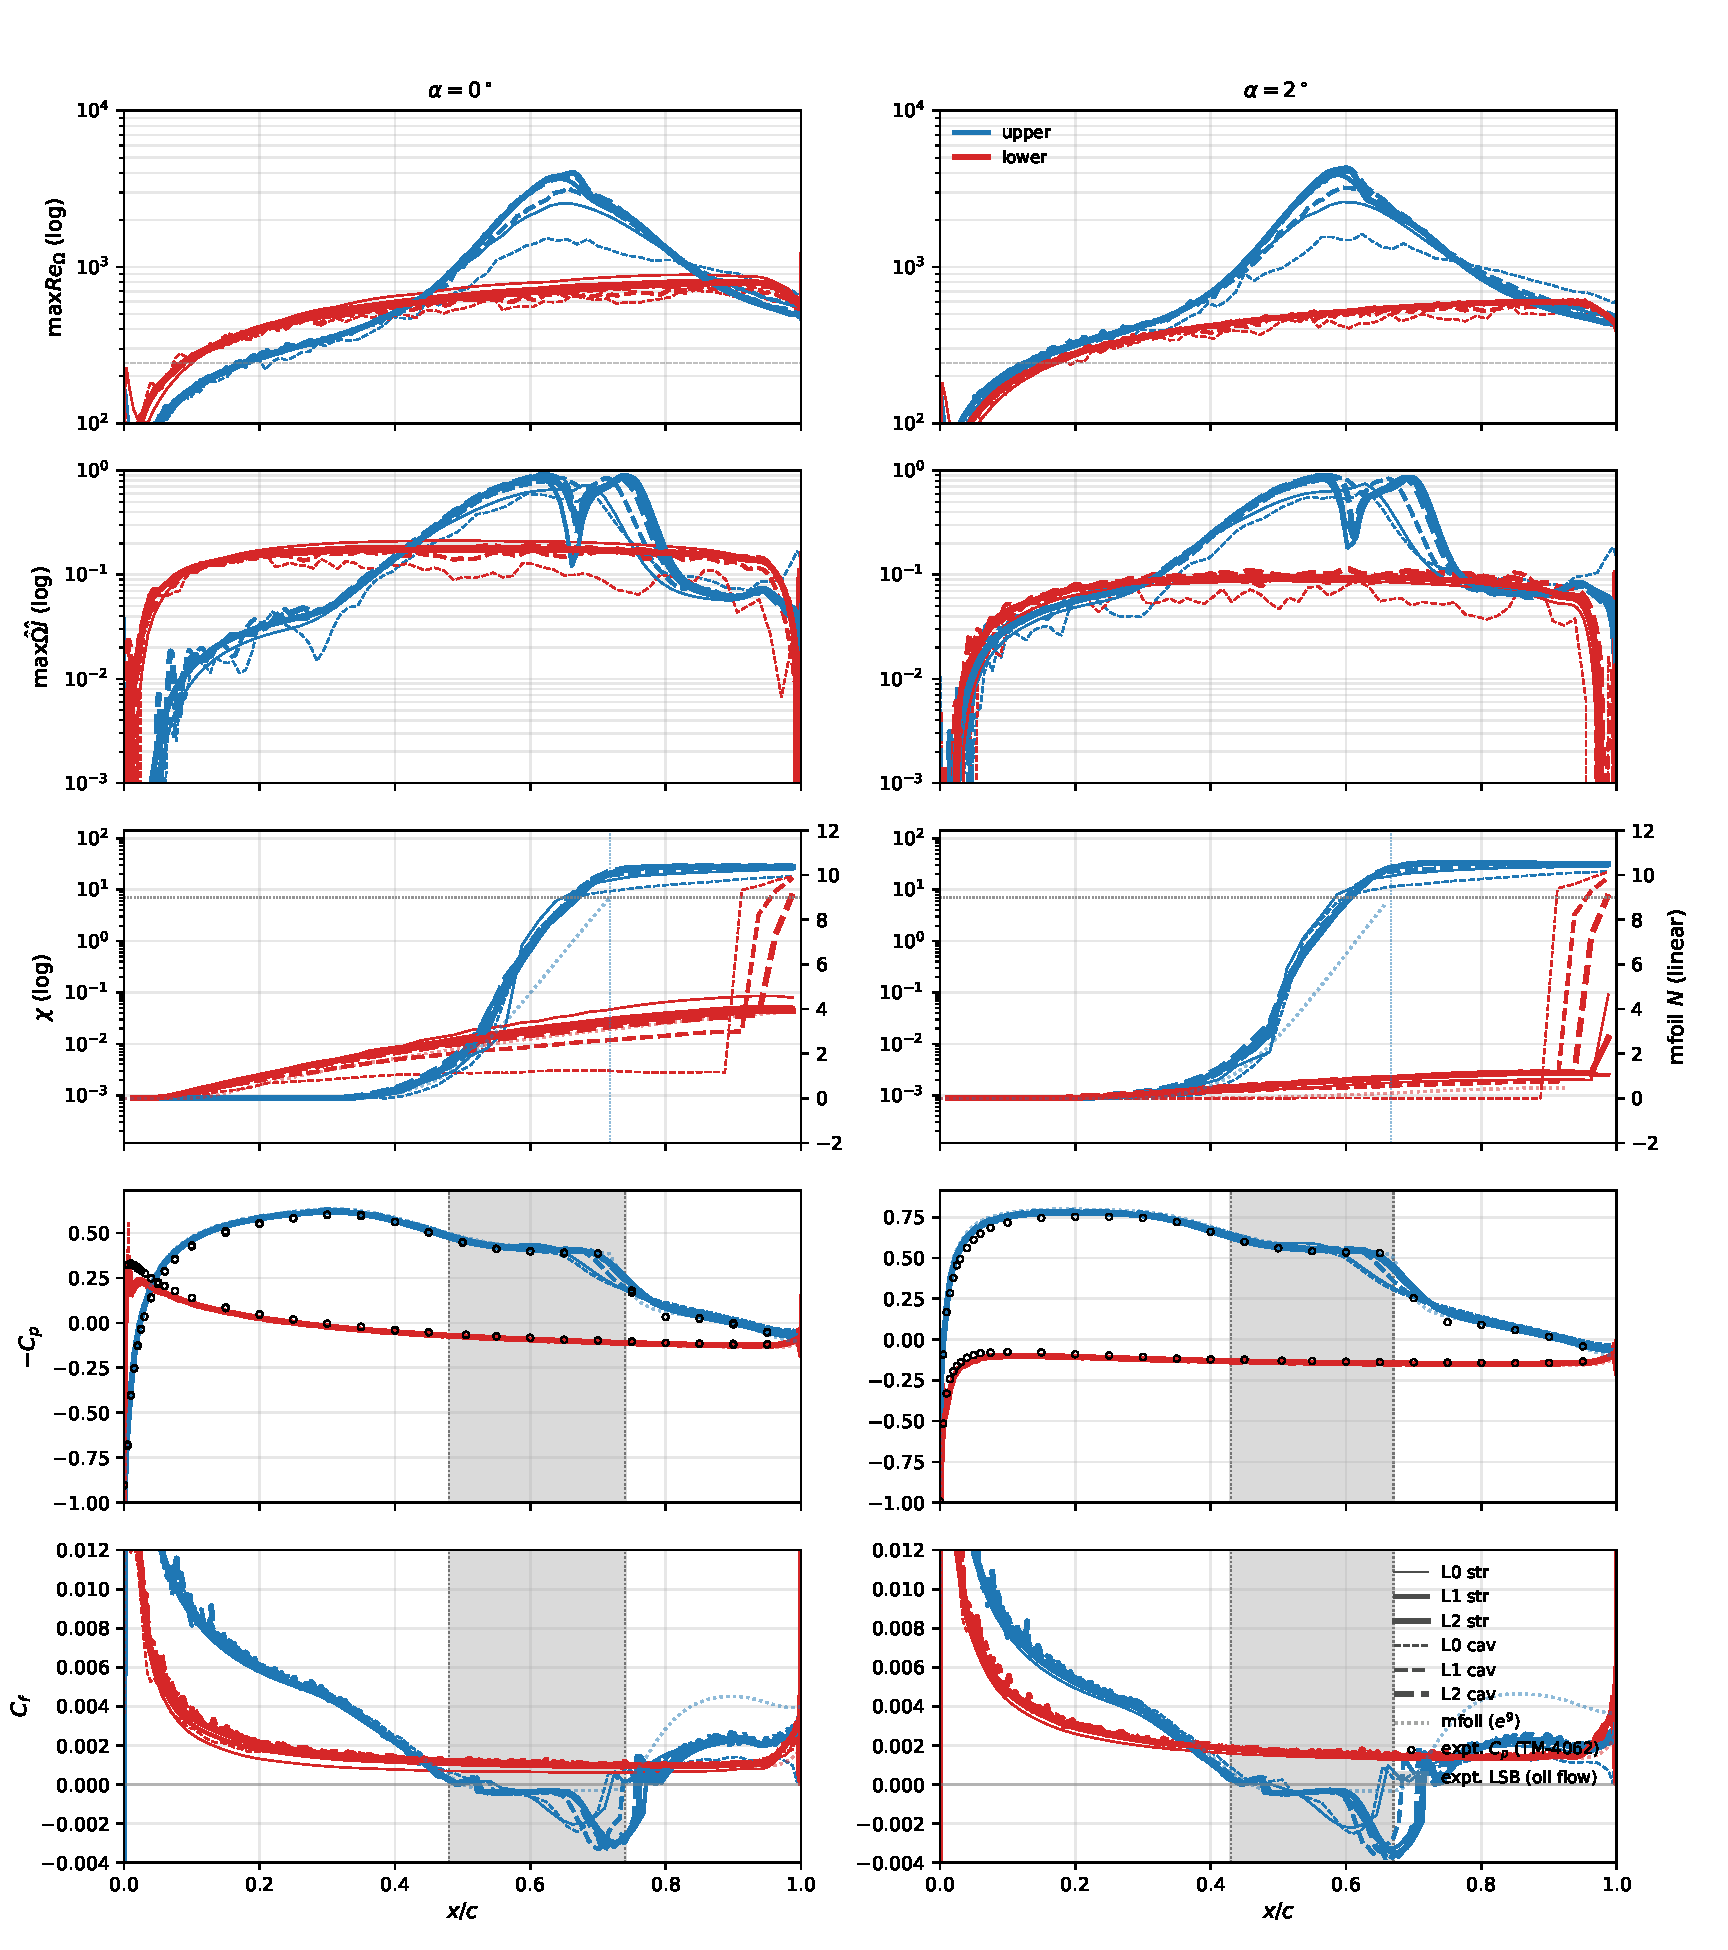
\includegraphics[width=0.99\textwidth]{eppler_cf_lowalpha.pdf}
  \caption{Eppler 387 surface distributions at $\alpha\!\in\!\{0^\circ,5^\circ\}$,
  $Re\!=\!2\!\times\!10^5$, $M\!=\!0.1$, $\chi_\infty\!=\!8.76\!\times\!10^{-4}$
  (matched to $N_\mathrm{crit}\!=\!9$). Five-row layout and line conventions as
  described in the text (row~1 $\max Re_\Omega$, row~2 $\max \hat\Omega \hat I$,
  row~3 $\chi$ with mfoil $N$, row~4 $-C_p$, row~5 signed $C_f$; upper blue /
  lower red, O-grid solid / cavity dashed, L0--L2 by thickness, mfoil $e^9$
  dotted, and the tabulated experimental $C_p$ (NASA TM-4062 App.~D, column with
  the nearest angle of attack) as open black circles on the $-C_p$ row). The signed $C_f$ (row~5) shows the laminar-separation bubble
  directly as the dip below zero on the upper surface. The bubble sits at
  $x/c\!\approx\!0.52$--$0.76$ at $\alpha\!=\!0^\circ$ and marches forward to
  $x/c\!\approx\!0.40$--$0.63$ at $\alpha\!=\!5^\circ$; both Flow360 and mfoil
  show the same recirculation structure.}
  \label{fig:eppcflow}
\end{figure}

\begin{figure}[tp]
  \centering
  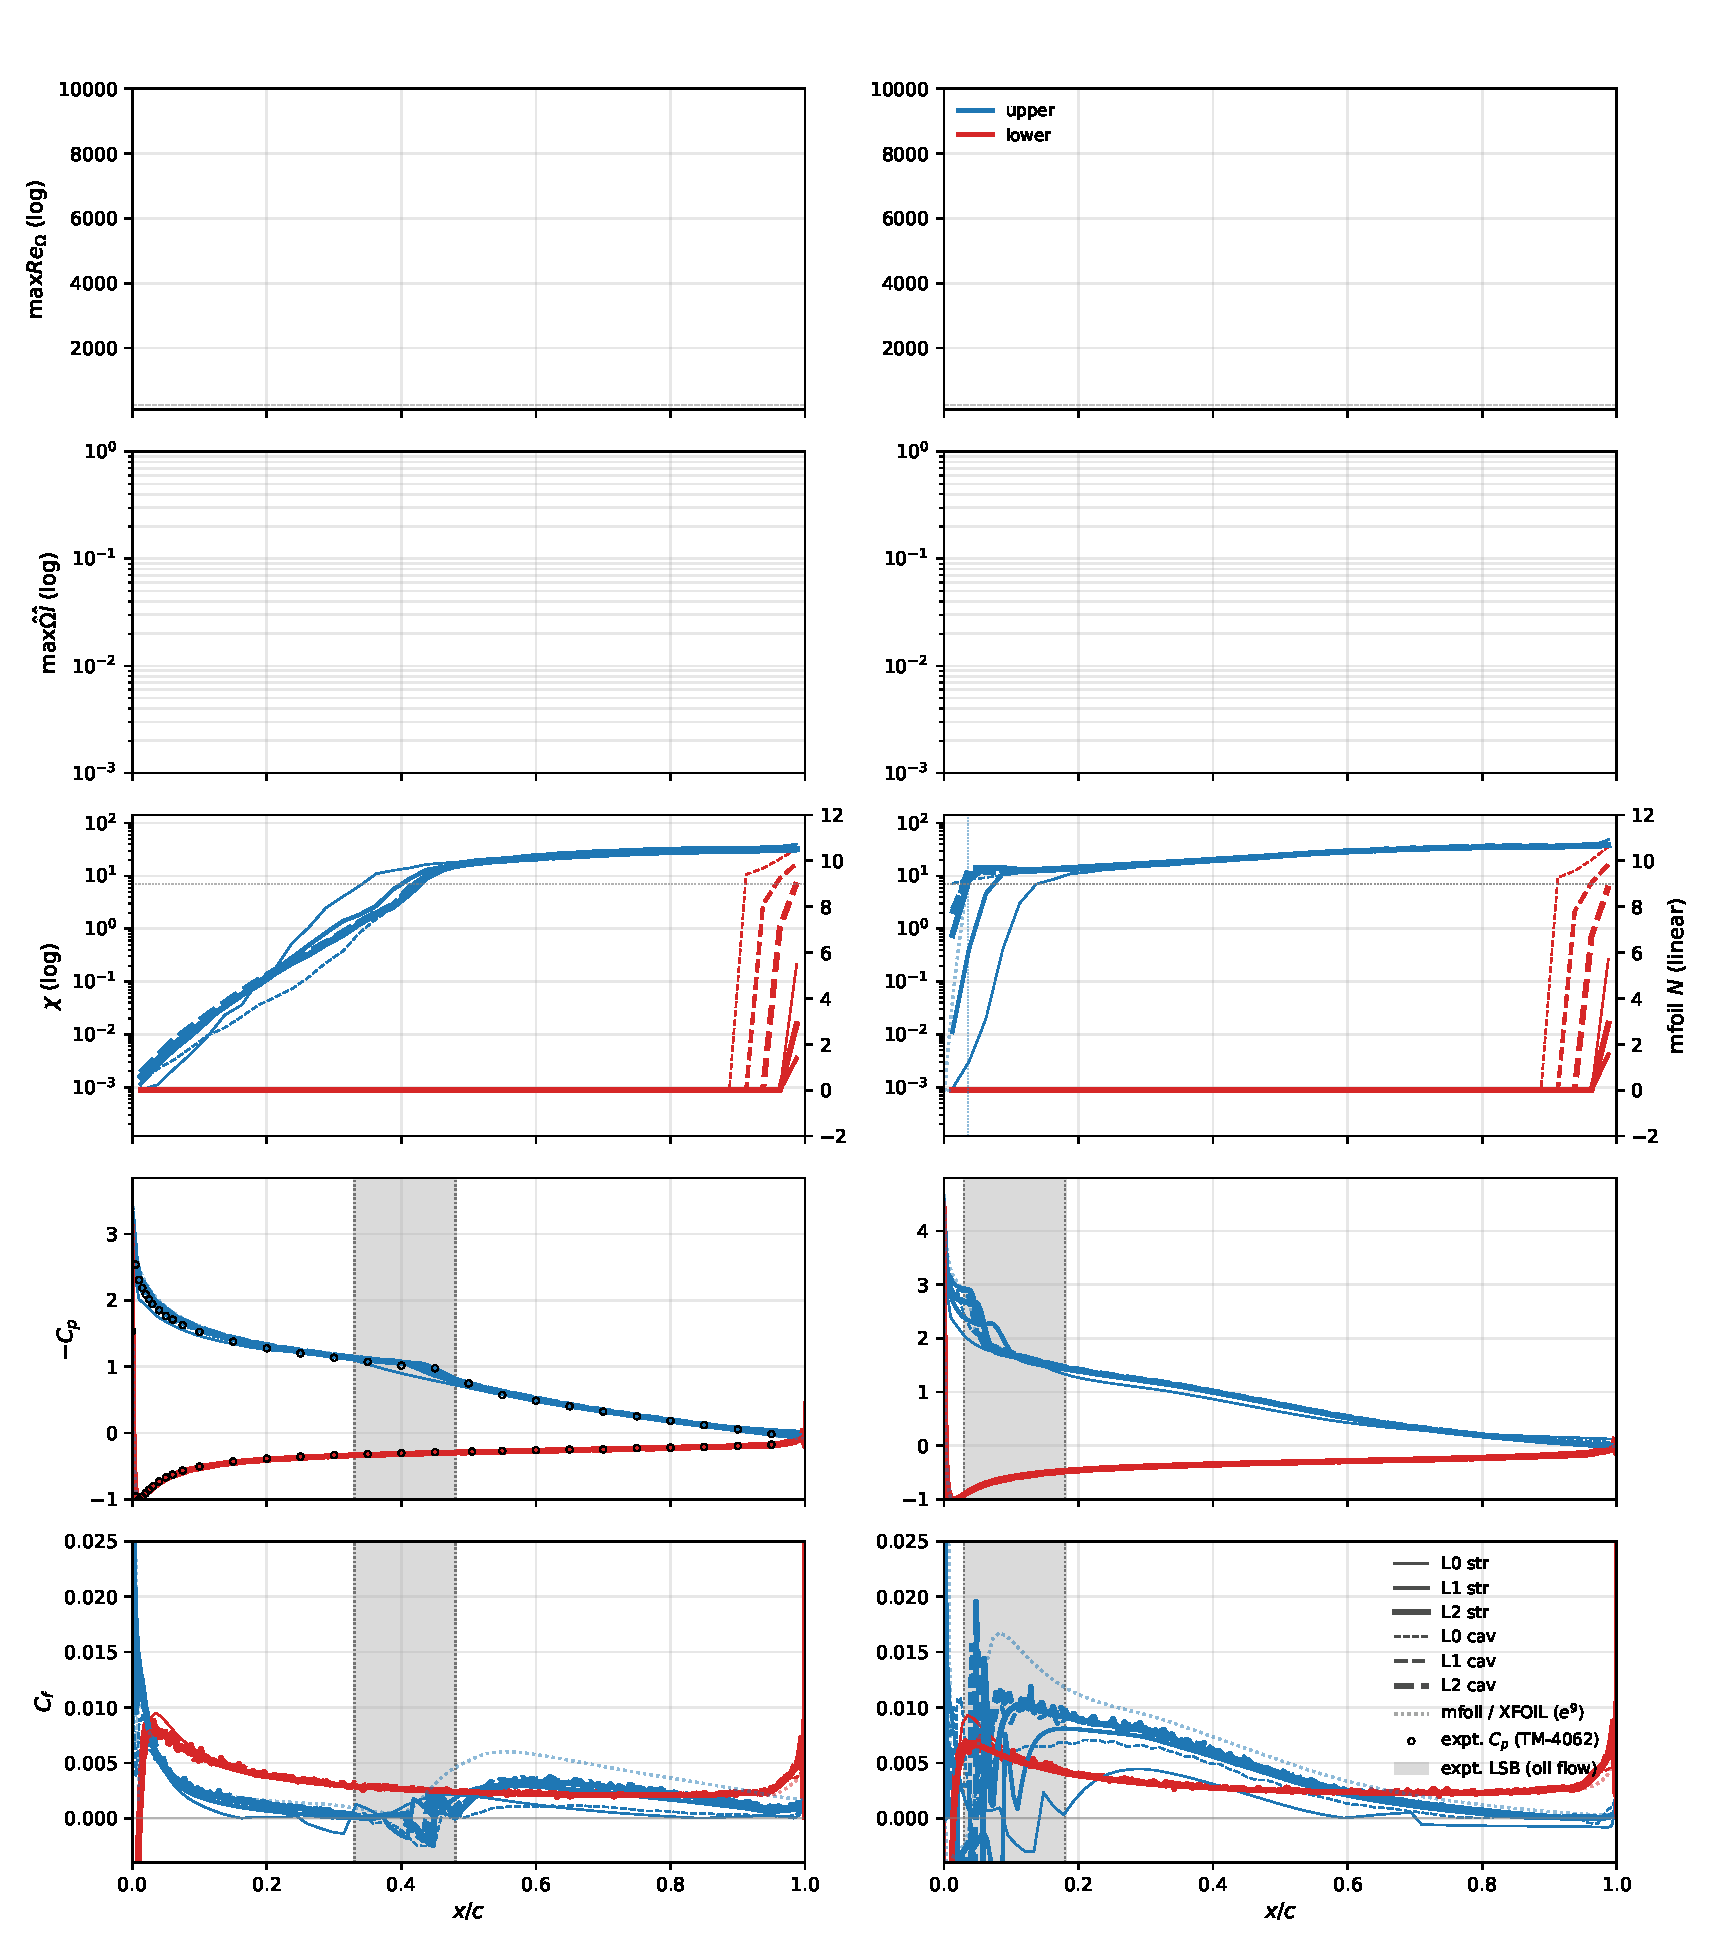
\includegraphics[width=0.99\textwidth]{eppler_cf_highalpha.pdf}
  \caption{As Fig.~\ref{fig:eppcflow}, at $\alpha\!\in\!\{7^\circ,8.5^\circ\}$
  ($8.5^\circ$ on the finest L2 pair only). At $\alpha\!=\!7^\circ$ the
  suction peak is near $-C_p\!\approx\!3$ and the model sits at the
  edge of bubble collapse: the upper-surface $C_f$ crosses zero only
  on three of the six grids (structured L0/L2 and cavity L0)---on the
  structured L2 a $x/c\!\approx\!0.39$--$0.41$ sliver, reattaching
  ${\sim}0.07\,c$ ahead of the measured oil-flow reattachment
  ($0.48\,c$)---while on the other three, transition preempts
  separation entirely, one incidence ahead of the experiment's
  $\alpha\!=\!8^\circ$ natural-transition point. At the post-stall
  $8.5^\circ$ both families trip in the leading-edge bubble (gray
  band: the oil flow's $0.03$--$0.18\,c$)---$\chi$ crosses $c_{v1}$
  within the first few percent of chord and the flow is turbulent and
  attached over the rest of the surface. The
  lower-surface boundary layer remains attached and laminar to
  $x/c\!\approx\!0.99$ across the entire $\alpha$ range, matching the
  $e^9$ prediction that the lower transition lies aft of the airfoil. At
  $\alpha\!=\!7^\circ$ the dotted reference is XFOIL rather than mfoil,
  which stalls numerically there (Fig.~\ref{fig:eppbubble});
  the surface distributions carry no $N$ curve, so
  row~3 shows no envelope at $7^\circ$ (at $8.5^\circ$ mfoil converges
  and the envelope returns). XFOIL's dumped $C_f$ is
  edge-normalized and is converted to the freestream convention of the
  computed rows ($\times u_e^2$).}
  \label{fig:eppcfhigh}
\end{figure}

The skin friction (Figs.~\ref{fig:eppcflow}--\ref{fig:eppcfhigh}, bottom rows)
shows the LSB directly: the upper-surface $C_f$ drops below zero over a band
that spans up to $\sim\!0.25\,c$ at low incidence---a shallow laminar separation
feeding a compact turbulent recirculation core---and collapses toward
$\alpha\!=\!7^\circ$, where only three of the six grids retain a
sliver of recirculation ($0.014\,c$ on the structured L2) and the
rest transition ahead of separation. Both
Flow360 and mfoil show the same recirculation structure at
$\alpha\!\le\!5^\circ$ on both mesh families.

The rate coordinate $\max_y \hat\Omega \hat I$ (row~2 of
Figs.~\ref{fig:eppcflow}--\ref{fig:eppcfhigh}) shows the adverse-gradient
response the Eppler~387 probes: on the upper surface $\hat\Omega \hat I$ rises from near zero
(the attached, near-neutral layer) into the strongly amplifying range across
the laminar-separation bubble (the inflectional profile), then relaxes after
reattachment, while the lower surface stays near zero; the growth of $\hat\Omega \hat I$ into
the amplifying region is what ignites transition at the bubble.
(The conspicuous double peak the upper-surface trace shows inside the
bubble---and the sharp notch between the two---is anatomized in
Appendix~B against the contour sheet of
Fig.~\ref{fig:sheet_eppler387_a5_upper}.)

\begin{figure}[tp]
  \centering
  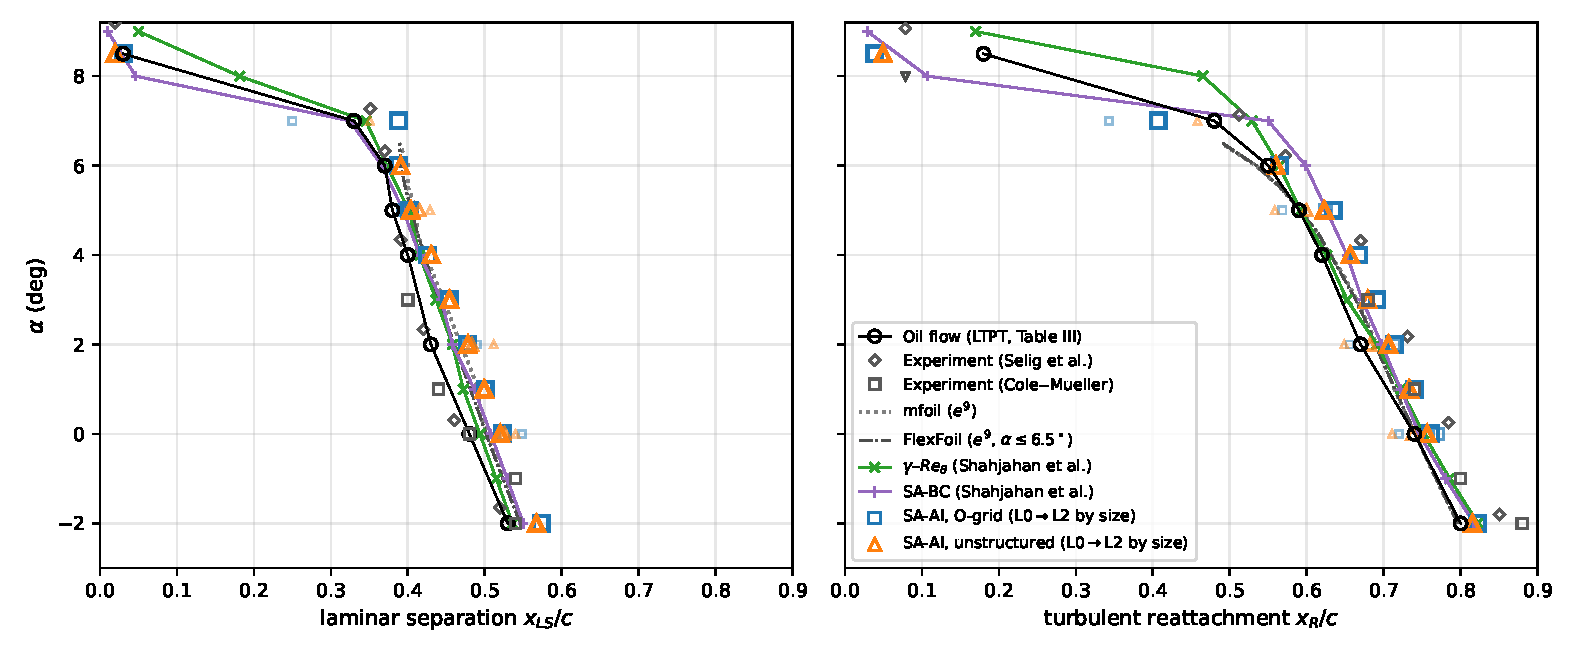
\includegraphics[width=\textwidth]{eppler_bubble_stations.pdf}
  \caption{Upper-surface laminar-separation (left) and
  turbulent-\emph{reattachment} (right) locations on the Eppler 387 at
  $Re\!=\!2\!\times\!10^5$ against incidence. For a laminar-separation
  bubble the physically observable stations are the separation and
  reattachment points, not the amplification onset; in the computation
  they are the signed-$C_f$ zero crossings (separation: first downward;
  reattachment: most-downstream upward---the physical return of
  attached flow aft of the bubble), and the same measure is taken from
  the $e^9$ references: mfoil (dotted; drawn to $\alpha\!=\!6.5^\circ$,
  beyond which it is at the edge of its convergence regime---at
  $\alpha\!=\!7^\circ$ it returns $C_l\!=\!0.928$, below its $5^\circ$
  value, while XFOIL~\cite{drela_xfoil_1989} converges there with
  $C_l\!=\!1.17$) and FlexFoil, a separate implementation of the
  same method (dash-dot). Past $\alpha\!=\!6.5^\circ$ the $e^9$
  closure \emph{transitions ahead of laminar separation}---its signed
  $C_f$ never crosses zero (FlexFoil and XFOIL agree, minimum
  $+4.7\!\times\!10^{-4}$ in the freestream convention at $7^\circ$)---and so predicts no bubble
  where the oil flow still shows one; the isolated FlexFoil marker at
  $8^\circ$ is a marginal three-point sliver. Black circles: the oil-flow visualization (McGhee et
  al., NASA TM 4062, Table~III; its nine tabulated incidences less
  $\alpha\!=\!8^\circ$, where the report notes natural transition at
  $0.32\,c$ and no bubble exists to plot---the $8.5^\circ$ point is
  the post-stall leading-edge bubble), i.e.\ the edges of the gray band on the $C_f$
  rows of Figs.~\ref{fig:eppcflow}--\ref{fig:eppcfhigh}. Gray diamonds:
  the independent Selig et al.\ measurement, digitized with the
  $\gamma$--$Re_\theta$ and SA-BC curves from
  Ref.~\cite{shahjahan_2024}
  (\texttt{data/lmbcm\_eppler387\_digitized.json}). Larger gray
  squares: the Cole--Mueller pressure-station
  measurements~\cite{cole_mueller_1990} at the same Reynolds number
  ($\pm1\%$ chord; their $\alpha\!\ge\!7^\circ$ entries are
  attached-transition values and plot no bubble). Open
  squares/triangles: SA-AI on all six grids (L0--L2 by marker size,
  both families); as on the polar, the $-2^\circ$--$8.5^\circ$
  extension incidences exist on the finest (L2) pair only, L0/L1
  keeping $\alpha\!\in\!\{0^\circ,2^\circ,5^\circ,7^\circ\}$. The
  lower surface stays attached and laminar to the
  trailing edge at every incidence.}
  \label{fig:eppbubble}
\end{figure}

The bubble stations are collected in Fig.~\ref{fig:eppbubble},
against the oil flow at its eight bubble incidences (the ninth,
$\alpha\!=\!8^\circ$, is natural transition with no bubble to
plot), the
independent Selig et al.\ measurement, the dense-$\alpha$ mfoil
sweep, and the two digitized transition-model references. The
separation location is
reproduced by every method on the plot, SA-AI included, to a few
percent of chord at every incidence. The reattachment---the bubble's
aft end, set by the post-transition turbulent recovery---is the
quantity this test hinges on, and it is where the model shows
its cost: at $\alpha\!\le\!5^\circ$, at grid convergence, both
families reattach late against the oil flow---a bubble
$0.02$--$0.04\,c$ too long---while at the near-stall $7^\circ$
the model sits at the edge of bubble collapse: three of six grids
(the unstructured finest among them) transition ahead of separation
and plot no stations---one incidence ahead of the experiment's
$\alpha\!=\!8^\circ$ natural-transition point---and the surviving
structured-L2 sliver closes $0.07\,c$ early; the lower surface runs
laminar to the trailing edge at every incidence and has no front to
move. That margin sits
\emph{inside} the facility-to-facility spread on the figure: the
Cole--Mueller pressure-station measurements at the same Reynolds
number~\cite{cole_mueller_1990} read reattachment $0.03$--$0.08\,c$
aft of the LTPT oil flow at and between its tabulated incidences
($\alpha\!=\!-2^\circ$--$3^\circ$; the oil flow interpolated where
the incidences do not coincide).

Past stall the trend continues: at the $8.5^\circ$ extension both
families reproduce the experiment's post-stall
\emph{leading-edge-bubble topology} (oil flow: separation at
$0.03\,c$, reattachment at $0.18\,c$) but reattach at
$0.032$--$0.049\,c$---roughly four times short of the measured
recovery---carrying the $\alpha\!\ge\!7^\circ$ early-reattachment
direction through the stall. The structured family's bubble is a
marginal few-sample sliver, and the solutions there are unsteady;
Fig.~\ref{fig:eppbubble} plots the stations of the time-median
surface solution.


This low-$\alpha$ over-length is not an amplification deficit: the
$\chi\!=\!1$ front sits mid-bubble,
slightly \emph{ahead} of the $e^9$ crossing
(Figs.~\ref{fig:eppcflow}--\ref{fig:eppcfhigh}, row~3), and the inflectional
profile saturates the rate coordinate ($\hat\Omega \hat I\!\approx\!1$) across the
mid-bubble. What is slow is the \emph{transition} itself: the
model carries no closure for the transition process, so
breakdown is represented by the transported-$\chi$ handover into SA
production, and the handover needs a fixed number of $e$-folds of
$\chi$ (${\approx}\ln c_{v1}$ to half commitment) whose physical
length is macroscopic at this Reynolds number. The turbulent stress
that closes the bubble therefore arrives aft of where spot-driven
breakdown completes in the tunnel, and reattachment---the quantity the
oil flow measures---lands $0.02$--$0.04\,c$ late even though the
front is placed correctly. Where that handover length leads as the
Reynolds number falls---to a bursting boundary, and to the loss of the
two-state structure the experiment shows---is the subject of the next
section, which quantifies it against the room the bubble has
(Sec.~\ref{sec:epphandover}).

\section{Reynolds-number study of the Eppler 387 at $\alpha\!=\!5^\circ$}\label{sec:eppresweep}

To assess whether the same constants follow the bubble across the
Reynolds-number range of the McGhee experiment, we hold everything of
Sec.~\ref{sec:eppval}'s study fixed---the incidence at
$\alpha\!=\!5^\circ$ and the freestream seed at
$\chi_\infty\!=\!8.76\!\times\!10^{-4}$---and sweep the four other tabulated
Reynolds numbers,
$Re\!\in\!\{6\!\times\!10^4,\,1\!\times\!10^5,\,3\!\times\!10^5,\,4.6\!\times\!10^5\}$,
reusing the grids of both mesh families at all three refinement levels
from the $Re\!=\!2\!\times\!10^5$
study unchanged (only the reference viscosity changes)---$24$ solutions
in all.
Figures~\ref{fig:eppresweep_low} and~\ref{fig:eppresweep_high} show the resulting
$-C_p$ and signed $C_f$, overlaid with the exact experimental surface pressures
(open markers, from the NASA TM-4062 Appendix~D tables at the column with the
nearest angle of attack---every repeat dataset the report holds at these
conditions) and the mfoil/XFOIL $e^9$ reference where it converges;
wall-anchored contour sheets for every solution of the sweep appear in
Appendix~C.
Every solution away from $10^5$ is steady---force coefficients flat
to $\Delta C_l\!\le\!3\!\times\!10^{-4}$ over the final $2000$
pseudo-steps, most below $10^{-4}$ (the loosest are the structured L1
benchmark at $2.6\!\times\!10^{-4}$ and the structured L0 at
$3\!\times\!10^5$ at $1.8\!\times\!10^{-4}$). At $10^5$, the
near-bursting condition discussed below, the cavity family carries
the residual unsteadiness ($\Delta C_l\!\approx\!3\!\times\!10^{-4}$
at L1, $7\!\times\!10^{-4}$ at L2) while the structured grids sit
at $\le\!3\!\times\!10^{-5}$; the structured-L1 bubble limit cycle
of the pre-bypass model does not recur under the recomputation.



The section lift, drag, and quarter-chord pitching-moment
coefficients are collected in Fig.~\ref{fig:eppresweepforces}, and
tabulated at L2 against the $e^9$ reference and the tunnel data in
Table~\ref{tab:eppresweep} (Appendix~C). The $e^9$ reference itself is
cross-checked: XFOIL (repaneled) and FlexFoil (a separately written
Rust implementation of the XFOIL closure set) were run at every
condition where mfoil serves as the reference in this paper, and the
three implementations agree to better than $1\%$ everywhere except
$Re\!=\!6\!\times\!10^4$, where mfoil visibly departs from the other
two; XFOIL---whose forces also sit closest to the measurement---is
presented as the reference there, in the table (mfoil in the footnote)
and in Fig.~\ref{fig:eppresweep_low}. \begin{figure}[tp]
  \centering
  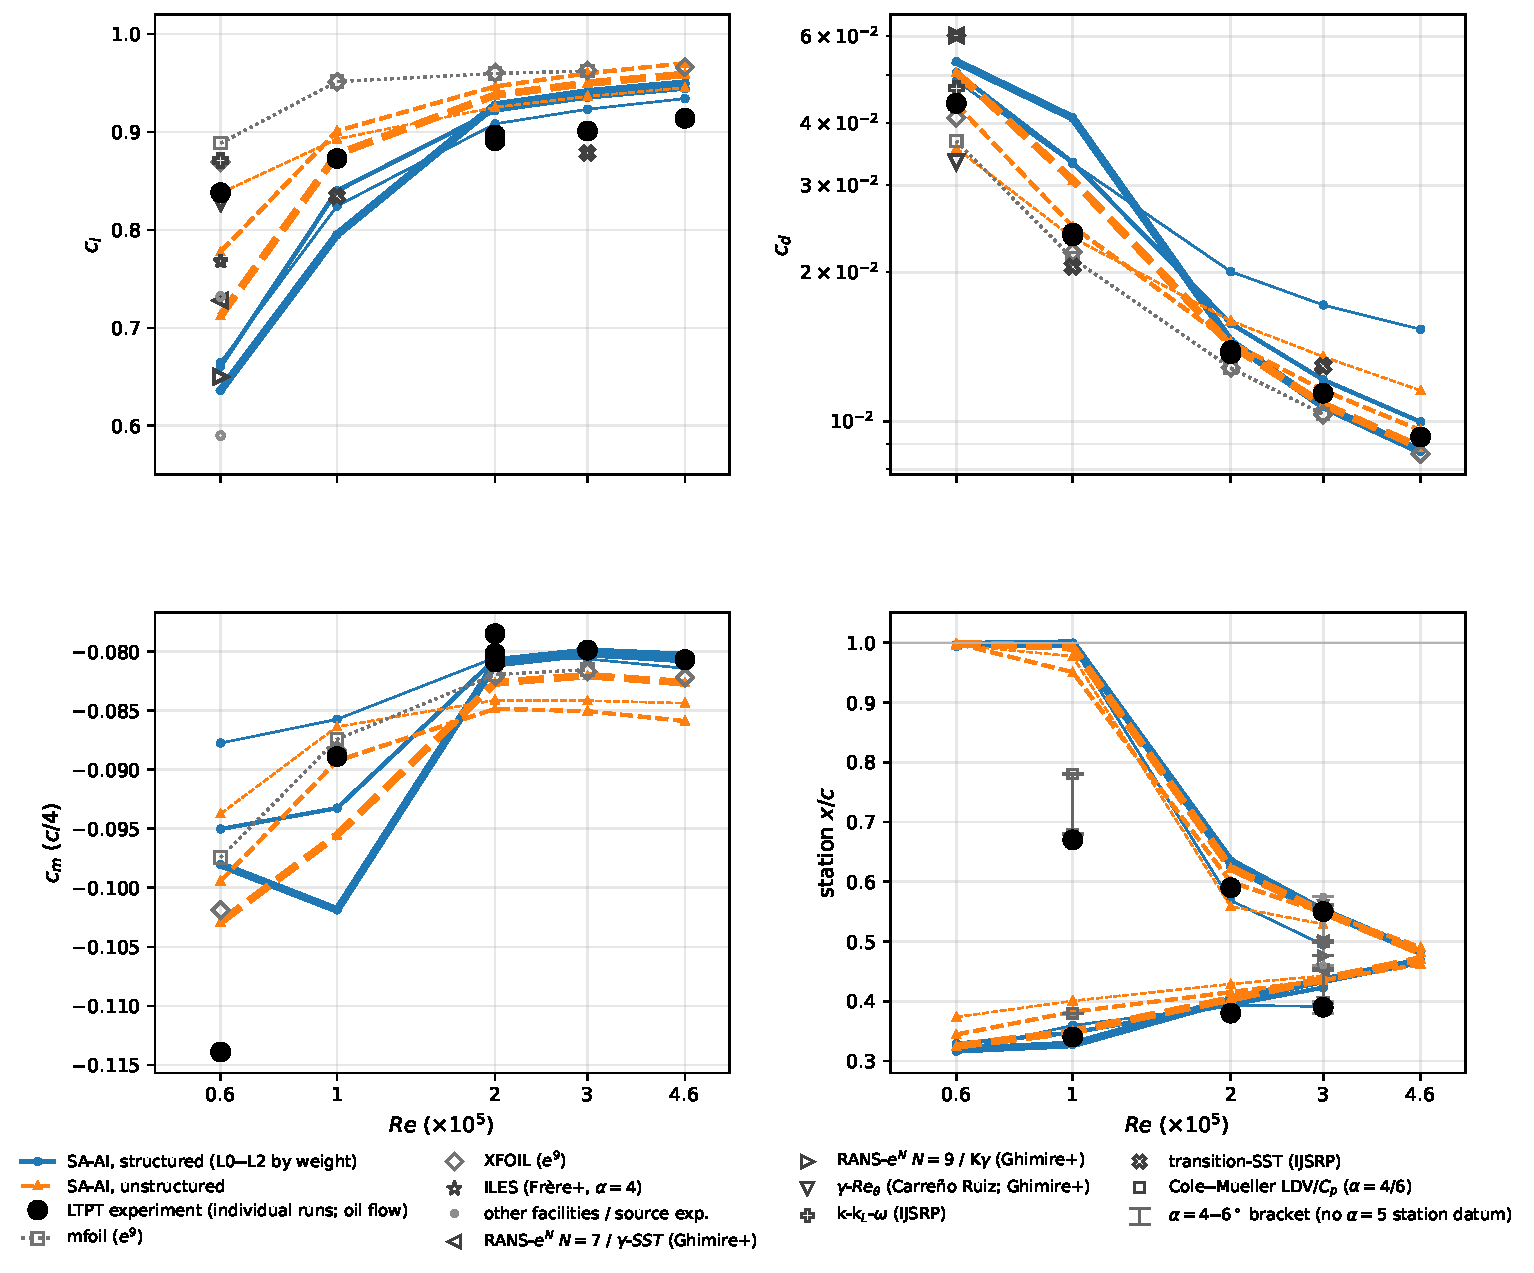
\includegraphics[width=\textwidth]{eppler_resweep_forces.pdf}
  \caption{The $\alpha\!=\!5^\circ$ Reynolds sweep. \emph{Top row}:
  section lift, drag (log), and quarter-chord moment---all $24$ SA-AI
  solutions (structured O-grid solid blue, unstructured cavity dashed
  orange, L0--L2 by line thickness), the $e^9$ panel reference (mfoil
  squares at $0.6$--$3\!\times\!10^5$, where its solve returns
  forces, XFOIL diamonds at all five Reynolds numbers,
  as in Table~\ref{tab:eppresweep}; $c_m$ from both), and the LTPT
  measurement (black circles; error bars are the repeat scatter,
  $\pm0.006$/$\pm0.0003$ at $Re\!\geq\!10^5$ and the
  $\alpha\!=\!4.00^\circ$ repeat half-spread $\pm0.04$/$\pm0.0023$
  at the bistable $6\!\times\!10^4$). Small dark-gray open symbols:
  published results at the shared conditions, read at
  $\alpha\!=\!5^\circ$---at $6\!\times\!10^4$ the ILES
  ($\alpha\!=\!4^\circ$, ahead of its reattachment jump) and coupled
  RANS-$e^N$ ($N\!=\!7/9$) of Ref.~\cite{frere_2016}, with that
  source's compiled Delft and Stuttgart $\alpha\!=\!5^\circ$ lift
  points (small dots), the $\gamma$--$Re_\theta$ of
  Ref.~\cite{carreno_ruiz_2022}, and the k-k$_L$-$\omega$ of
  Ref.~\cite{anushka_2019}, whose transition-SST appears at $1$ and
  $3\!\times\!10^5$ (its $6\!\times\!10^4$ series and as-plotted
  experiment are corrupt in the source and excluded;
  \texttt{data/ijsrp2019\_e387\_polars.json}). \emph{Bottom row}:
  upper-surface laminar-separation and turbulent-reattachment stations
  (SA-AI from the wall $C_f$; values pinned near $1.0$ mean no closure
  ahead of the trailing edge), the oil flow (open black circles,
  TM-4062 Table~III), the Cole--Mueller pressure/LDV stations at
  $10^5$~\cite{cole_mueller_1990} ($\alpha\!=\!4^\circ/6^\circ$
  bracket pair, connected), and the tabulated $\gamma$-variant
  stations of Ref.~\cite{ghimire_2025} at $3\!\times\!10^5$ (same
  bracket convention; small gray dots are that source's experiment
  columns). The refinement fan closes onto the measurement at
  $2$--$4.6\!\times\!10^5$ and \emph{opens} at $10^5$---the model's
  bursting boundary (Sec.~\ref{sec:epphandover})---where refinement
  drives both families away from the measured short-bubble state.}
  \label{fig:eppresweepforces}
\end{figure}

The one
systematic failure is at $Re\!=\!10^5$, where the computation sits past
the model's bursting boundary (the opening fan of
Fig.~\ref{fig:eppresweepforces}): on every grid the upper-surface recovery
is incomplete---the signed $C_f$ regains zero only within $0.05\,c$ of
the trailing edge, against the measured oil-flow reattachment near
$0.67\,c$---and the L2 drag sits $+30\%$ (unstructured) to $+73\%$
(structured) above the measurement, refinement pushing both
families toward the burst state rather than the measured short bubble
(the coarser grids only mask the failure: the unstructured L1 lands
$+4\%$ high).
The over-length has two contributions---the under-amplified detached
shear layer of \S\ref{sec:calib_rate}, dominant at $2\!\times\!10^5$,
and the stretching handover zone of Sec.~\ref{sec:epphandover}, which
takes over as the Reynolds number falls: at this Reynolds number the
model's extended laminar separation fails to close at all.
The remainder of this section takes this failure apart: the computed state
is unique---every initialization converges to it, on relaxation times
an order of magnitude longer than anywhere else in the sweep---and
what makes that unique state the burst one is the length of the
model's transition zone. The measured pressures confirm
the computed bubble structure where the bubble does close: the
suction-side plateau of the separated shear layer appears in the
open-circle data at $3\!\times\!10^5$ exactly where the computed $C_p$
flattens, and at $10^5$ over the bubble's front half, before the
computed and measured recoveries part company.

The solution is markedly more mesh-sensitive at $6\!\times\!10^4$ than at
the higher Reynolds numbers: the open separation gives
$C_l\!=\!0.71$ unstructured vs.\ $0.64$ structured at L2, against
$\Delta C_d\!\leq\!2\!\times\!10^{-4}$ ($8\!\times\!10^{-4}$ at L1) at
$3$--$4.6\!\times\!10^5$.
The experiment itself is bistable there: in the TM-4062 listing at
$Re\!=\!6\!\times\!10^4$, three consecutive repeat points at
$\alpha\!=\!4.00^\circ$ give $c_l\!=\!0.643$, $0.697$, and $0.721$
($c_d\!=\!0.0431$, $0.0386$, $0.0400$), and the measured lift collapses from
$0.838$ at $\alpha\!=\!4.99^\circ$ to $0.639$ at
$\alpha\!=\!5.51^\circ$---run-to-run scatter of the same order as the spread
between the two computed solutions. The condition sits near the bubble-bursting limit, where the measurement
is bistable and the computation most mesh-sensitive
(the branch question is taken up below); the mesh scatter
and the offset from the
$e^9$ reference there reflect that regime together with the model's over-long
bubble (\S\ref{sec:calib_rate}) and the post-separation turbulent recovery, and
we claim only the macroscopic trend.

The sweep traces the classic low-$Re$ bubble progression at fixed incidence: as
the Reynolds number rises the transition front moves forward and the
laminar-separation bubble shortens. The upper-surface $C_f$ shows an open,
non-reattaching separation at $Re\!=\!6\!\times\!10^4$---the flow separates near
$x/c\!\approx\!0.32$ and does not recover ahead of the trailing edge, the
low-$Re$ bubble-bursting limit---then an incompletely closing
separation at $10^5$, the $C_f$ regaining zero only within $0.05\,c$ of
the trailing edge on every grid (the model carries the bursting regime
one Reynolds step past the measurement), and then short, shallow
bubbles---the computed $C_f$
only grazes zero---recovering, on the two finer levels, at
$x/c\!\approx\!0.55$ ($3\!\times\!10^5$) and
$x/c\!\approx\!0.48$
($4.6\!\times\!10^5$).

The deep reverse-$C_f$ surge inside the long bubbles at
$Re\!=\!6\!\times\!10^4$ and $10^5$ ($C_f\!\approx\!-0.005$, several
times the turbulent peak that follows) is qualitatively physical---bubble
DNS shows a sharp negative surge near the rear of strongly separated
bubbles~\cite{spalart_strelets_2000, alam_sandham_2000}---but its
magnitude is outside the model's declared scope: the mid-bubble $C_f$
profile is an uncalibrated byproduct of the $\sigma_t$ handover and of
standard SA's separated-flow behavior, and we claim no accuracy for it.
What this section tests is the macroscopic content: separation,
transition, reattachment, and the forces that follow.

\begin{figure}[tp]
  \centering
  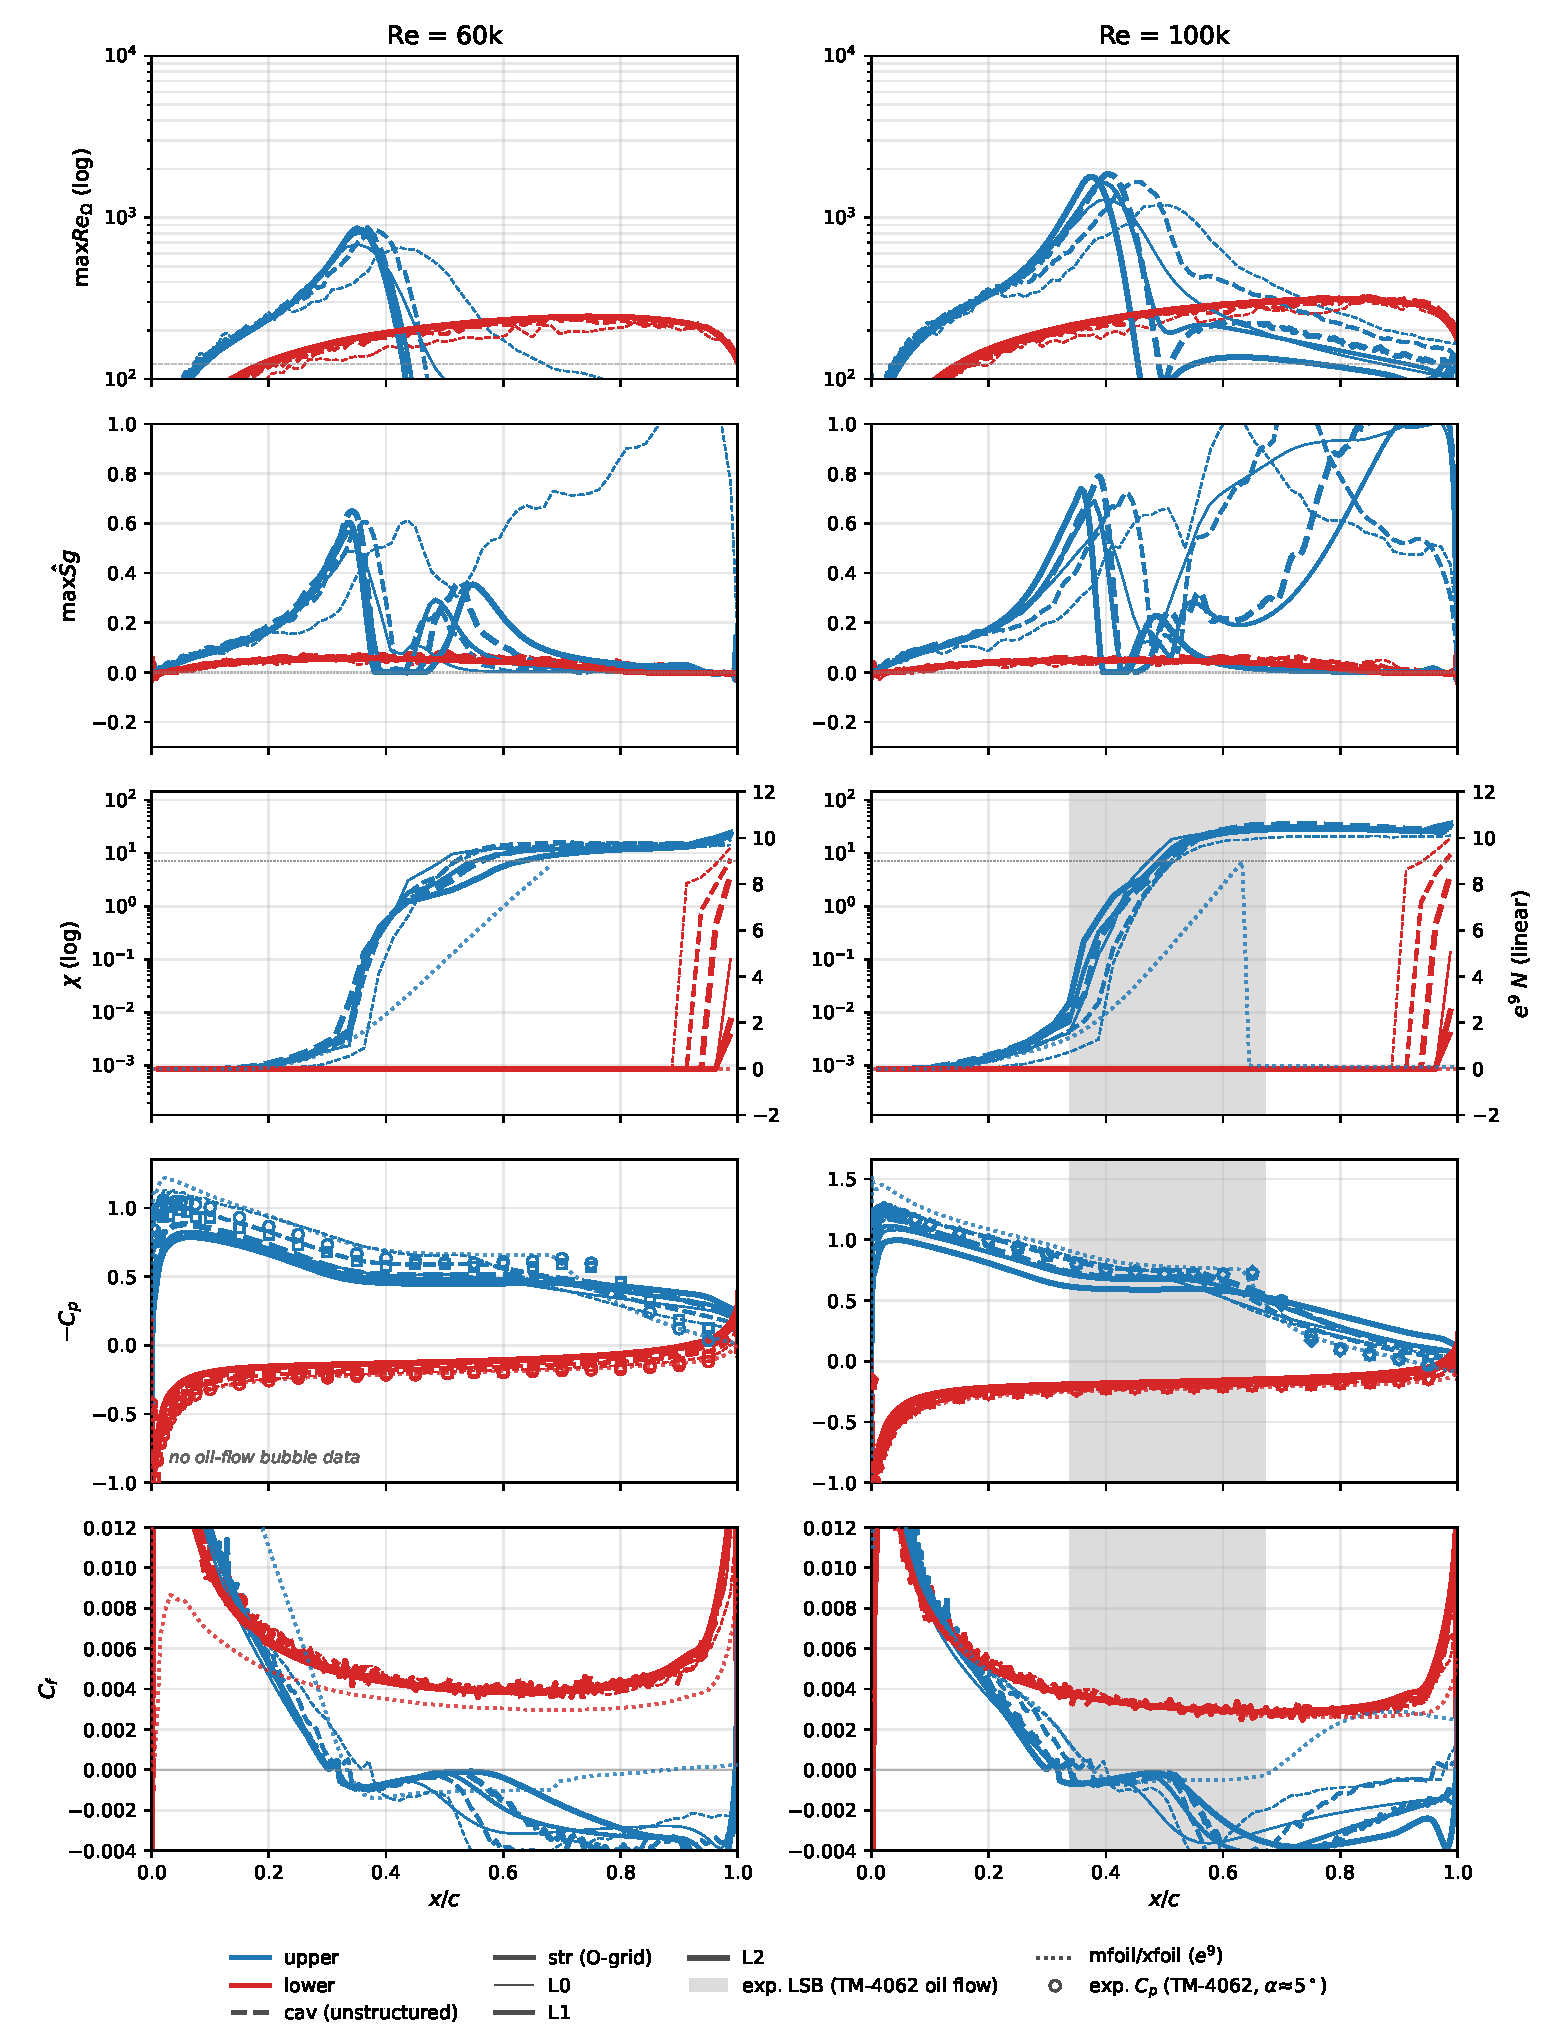
\includegraphics[width=\textwidth]{eppler_resweep_lowRe.pdf}
  \caption{Eppler 387 at $\alpha\!=\!5^\circ$, $Re\!=\!6\!\times\!10^4$ (left) and
  $1\!\times\!10^5$ (right): the five-row suite and line conventions of
  the benchmark figures (rows: $\max Re_\Omega$, $\max\hat\Omega \hat I$,
  $\max\chi$ with the $e^9$ $N$ envelope, $-C_p$, signed $C_f$), both
  mesh families, L0--L2 by line thickness. Dotted: the $e^9$
  reference---XFOIL at $6\!\times\!10^4$ (Table~\ref{tab:eppresweep}),
  mfoil at $10^5$; the $N$ envelope at $6\!\times\!10^4$ is
  FlexFoil's. Open markers: \emph{every} TM-4062 repeat pressure
  dataset at these conditions. At $6\!\times\!10^4$: circles the
  up-sweep, squares the decreasing-$\alpha$ hysteresis branch, whose
  weaker plateau and less complete recovery measure the experimental
  branch scatter at the bistable condition (see text). At $10^5$:
  circles/squares/diamonds are three tunnel conditions that coincide
  to repeat accuracy---the measured flow there is single-branch. Gray
  band: oil-flow bubble extent (TM-4062 Table~III; exists only at
  $10^5$ among these two). At $6\!\times\!10^4$ the computed
  separation does not reattach ahead of the trailing edge; at $10^5$
  the recovery is incomplete on every grid (see text).}
  \label{fig:eppresweep_low}
\end{figure}

\begin{figure}[tp]
  \centering
  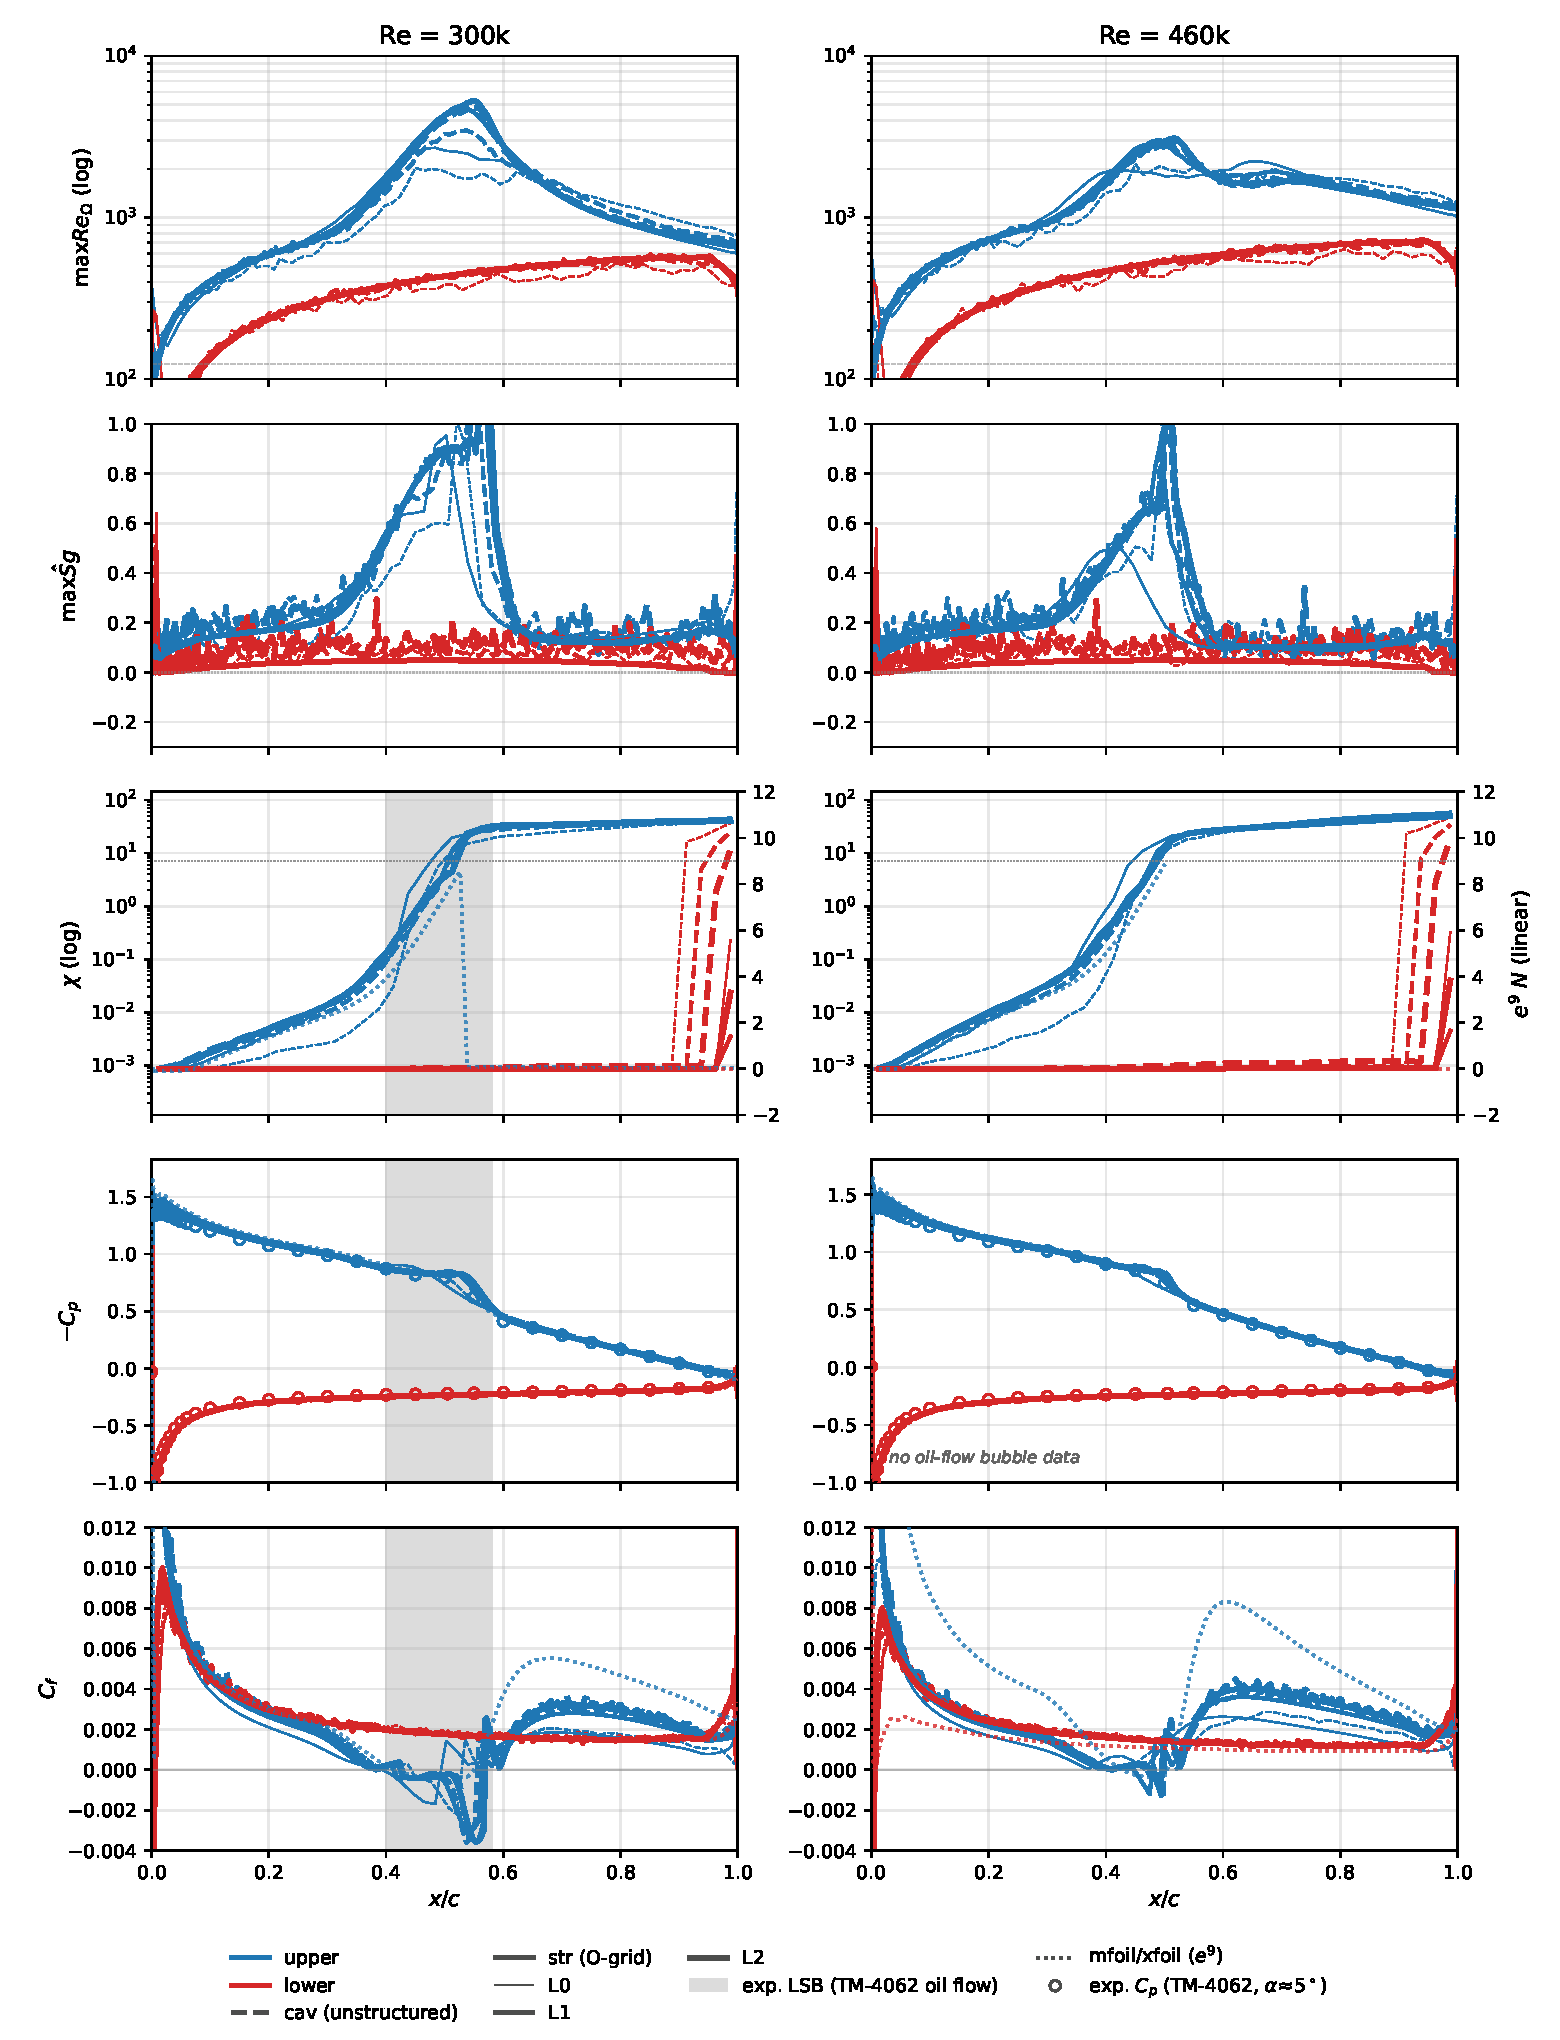
\includegraphics[width=\textwidth]{eppler_resweep_highRe.pdf}
  \caption{As Fig.~\ref{fig:eppresweep_low}, at $Re\!=\!3\!\times\!10^5$ (left) and
  $4.6\!\times\!10^5$ (right). The bubble is short and moves forward with Reynolds
  number, recovering (on the two finer levels) near
  $x/c\!\approx\!0.56$--$0.57$ at $3\!\times\!10^5$ and
  $\approx\!0.48$ at $4.6\!\times\!10^5$ (at these two Reynolds
  numbers the computed $C_f$ only grazes zero). The mfoil $e^9$ panel solver converges at
  $3\!\times\!10^5$ but diverges on the thin bubble at $4.6\!\times\!10^5$, where
  XFOIL supplies the $e^9$ $C_p$/$C_f$ reference (dotted) and FlexFoil the
  $N$ envelope ($\chi$ row) instead. The oil-flow bubble band is available at
  $3\!\times\!10^5$ only.}
  \label{fig:eppresweep_high}
\end{figure}

\phantomsection\label{sec:eppbistab}The measured flow is itself two-valued at
$6\!\times\!10^4$: the LTPT observed laminar separation with and
without turbulent reattachment at the same angle of attack over
$\alpha\!\approx\!3^\circ$--$7^\circ$ (McGhee et al.'s Fig.~11(a)), the
selection was environmental (at the slightly noisier tunnel condition
the flow always failed to reattach), repeat polars scatter an order of
magnitude more than at any higher Reynolds number
(Table~\ref{tab:eppresweep}), and the decreasing-$\alpha$ hysteresis
runs read a measurably weaker, less-recovered upper surface than the
up-sweep at the same angle ($\Delta C_p$ rms $0.06$, four times the
repeat scatter; squares vs.\ circles in
Fig.~\ref{fig:eppresweep_low})---while above $6\!\times\!10^4$
``turbulent reattachment always resulted'' and the $10^5$ repeat
conditions coincide. The model reproduces neither the second branch
nor the hysteresis: direct forks of each family's converged
$2\!\times\!10^5$ solution, slow one-step Reynolds descents and
climbs, and $40\,000$-iteration extensions of every $10^5$ endpoint
all converge to one family-specific state at $10^5$ (structured:
lift agreeing to $\le\!0.003$, drag to ${\approx}5\!\times\!10^{-4}$;
cavity: $\le\!0.005$ among cold, fork, and descent, with the slow
climb still $0.012$ away and drifting toward the pack at the end of
its $40\,000$-iteration extension) and collapse onto the burst branch
at $6\!\times\!10^4$
(repro: \texttt{repro/cfd/run\_bistability\_forks.py},
\texttt{run\_continuation\_ladders.py}, \texttt{run\_fork\_extensions.py},
\texttt{run\_dn\_extensions.py}; the probes were repeated in full at
the recomputed canon and the conclusion carried over). \emph{The
model is monostable throughout the sweep}; the only trace of the nearby fold is the
relaxation time at $10^5$---the warm-started paths need their full
$4\!\times\!10^4$-iteration extensions to close on the cold state
(the cavity climb is still drifting at the end of its), an order of
magnitude longer than anywhere else in the sweep---and the experiment's two-state structure, hysteresis included,
lives at $6\!\times\!10^4$, one Reynolds step below the model's
bistable-free burst.

\phantomsection\label{sec:epphandover}Why does the model burst where the
measurement reattaches? The account begun at the $2\!\times\!10^5$
benchmark (Sec.~\ref{sec:eppval})---separation on time, the front on
time to early, reattachment late---completes here as a length scale.
The handover from amplification to SA production must climb a fixed
number of $e$-folds of $\chi$: $\ln c_{v1}\!\approx\!2.0$ from the
$\chi\!=\!1$ crossing to eddy-viscosity half-saturation, another
$\approx\!1.4$ to effectively full production. The length one
$e$-fold costs, roughly $u_\mathrm{conv}/(a\,\omega)$, is not fixed:
it stretches like $\delta/c\!\propto\!Re^{-1/2}$ as the layers
thicken, and faster once the bubble grows. Measured on the computed
structured-L2 solutions
(repro: \texttt{repro/cfd/analyze\_handover\_length.py}), the
half-saturation length is $0.025$--$0.05\,c$ at $2$--$4.6\!\times\!10^5$,
where the bubble closes $0.04$--$0.15\,c$ past the crossing; at
$10^5$ half-saturation alone costs $0.05$--$0.10\,c$, full production
arrives only $0.18$--$0.30\,c$ downstream, and the bubble never closes;
at $6\!\times\!10^4$ full production is never reached on the airfoil.
The $e^9$ reference---whose closure switches to fully turbulent
\emph{at} the transition point---reattaches within $0.05\,c$ of its
transition station at $10^5$, on the measured reattachment, and
spot-driven breakdown in bubble DNS is similarly
abrupt~\cite{alam_sandham_2000, spalart_strelets_2000}. It is
therefore not the onset placement but the \emph{length of the modeled
transition zone}---the deliberately unphysical $\sigma_t$
interpolation---that starves the bubble of eddy viscosity, makes the
model's unique state the burst one, and pushes the bursting boundary
one Reynolds step above the measurement while erasing the two-state
structure the experiment shows at $6\!\times\!10^4$. Narrowing the
interpolation is not the remedy: at $\tau\!=\!1$ (a four-times-narrower
ramp) the handover becomes a relaxation oscillator---production closes
the bubble, closure destroys the amplification fetch that fired the
gate, and the bubble reopens---with $\Delta C_l\!\approx\!0.3$ at
$10^5$ and $\approx\!0.06$ even at the otherwise steady
$2\!\times\!10^5$ benchmark (cases
\texttt{tautest\_strL2\_Re\{100,200\}k\_a5\_tau1}, repeated at the
recomputed canon, where the oscillation persists). The gate is
memoryless where breakdown is irreversible. The identified remedy,
left to future work, is a transition-zone closure with physical
content: an outer-scaled breakdown trigger (a Reynolds-stress proxy
such as $\tilde\nu\omega/U^2$ reaching a mixing-layer saturation
level, in place of the molecular-units $\chi$ ladder) combined with
the transported memory of breakdown that spot-growth and
intermittency models carry.

The starved handover is one of \emph{two} low-Reynolds defects, and
the second runs in the opposite direction: below the bursting boundary
the amplification the model books inside the bubble outpaces the $e^N$
envelope. The mechanism is not the rate---the kernel's production in
the reversed ``dead air'' is onset-gated to effective zero---but the
topology of the transport: in the elliptic solution the bubble is a
closed cell, and $\tilde\nu$ produced in the shear layer diffuses
across it into the reversed stream, convects \emph{back upstream}, and
re-enters the amplifying band already elevated. Measured on the
structured-L2 sweep (\texttt{repro/cfd/measure\_lsb\_reseeding.py}),
the median $\chi$ in the reversed region over the bubble's first third
sits $21$--$27\times$ \emph{above} the incoming-envelope level just
upstream of separation at $Re\!\le\!10^5$, but $27\times$
\emph{below} it already at $2\!\times\!10^5$ and
$70$--$170\times$ below at $3$--$4.6\!\times\!10^5$; the flip is sharp at the
bursting boundary because the conducting overlap---an amplifying layer
running over un-closed reversed flow for half the chord---is itself
created by the starved handover, so the two defects are one causal
chain. The signature is readable directly in the $\chi$ sheets of
Appendix~C (Figs.~\ref{fig:sheet_eppler387_Re60k_upper}
and~\ref{fig:sheet_eppler387_Re460k_upper}): at low $Re$ the $\chi$
front is bottom-led---a cold front, the reversed flow carrying $\chi$
upstream along the wall---while at high $Re$ it is top-led, a warm
front riding the outer layer. No profile-based calibration can see
this defect: the frozen-profile instrument of
Sec.~\ref{sec:calib_rate} marches one-way by construction, and prices
the band's slow convection but not the spiral ledger path of a closed
cell.

The two defects meet, at the lowest Reynolds numbers, in a fortunate
cancellation, and the honest reading of this section is worth stating
plainly. At $2$--$4.6\!\times\!10^5$ both defects are small and the model
is genuine to the physics: the booked amplification tracks the $e^N$
envelope through bubbles and attached recoveries alike, and the
handover is short on the bubble's scale. At $Re\!\lesssim\!10^5$
the model still places separation and the transition front, and lands
within $11\%$ (family-dependently) on lift---but by
compensation: the re-seeded climb fires the $\chi\!=\!1$ front
$\sim\!0.16\,c$ \emph{ahead} of the physical envelope's equivalent
station (measured against the mfoil envelope at
$N\!=\!\ln(1/\chi_\infty)$: $0.41$ vs $0.57\,c$ at $10^5$,
$0.44$ vs $0.60\,c$ at $6\!\times\!10^4$), a head start that the
over-long handover then spends---and, below the boundary,
overspends---compounded by standard SA's own
low-$Re$ anemia: in a constant-stress layer the equilibrium
$\tilde\nu$ supports only $\chi\!\approx\!0.09\,Re_\tau$
(the friction-velocity Reynolds number;
\texttt{repro/analytic/sa\_sustain.py}), so at the $6\!\times\!10^4$
bubble shear
layer's $Re_\theta\!\approx\!220$--$330$ the reattached turbulence
would equilibrate near $\chi\!\sim\!c_{v1}$ with $f_{v1}$ only half
active. Low-$Re$ solutions
in this range should be read as the sum of two canceling errors, not
as resolved transition physics.


\section{Three-dimensional deployment: the Daedalus wing}\label{sec:daedalus}

(This section's campaign predates the lifted-layer bypass adoption of
\S\ref{sec:fv1bypass}; its recomputation is in progress, and every
number and figure here is from the bypass-inactive model.)

The model's first three-dimensional application is the wing of the
Daedalus human-powered aircraft: half-span $17.07\,$m, root chord
$0.917\,$m, aspect ratio $37.8$, Drela's DAE-11/21/31 low-Reynolds
sections~\cite{drela_daedalus_1988} blended along the span, constant
chord to $\eta\!=\!0.88$ and a straight taper to the tip. The operating
point is the aircraft's: $Re_\mathrm{root}\!=\!5\!\times\!10^5$,
$\alpha\!\in\!\{4^\circ,5^\circ,6^\circ\}$ spanning
$C_L\!\approx\!1.02$--$1.23$ about the design lift, with the flight-quiet
freestream seed $\chi_\infty\!=\!8.76\!\times\!10^{-6}$
($N_\mathrm{crit}\!\approx\!13.6$ by the map of
Sec.~\ref{sec:calib_tu}, the flight-environment amplification level of the
Daedalus design work~\cite{drela_daedalus_1988}). The solver and
kernel are exactly those of the airfoil studies: an earlier campaign
with a predecessor kernel (a shaped-rate variant whose onset threshold
lacked the in-bubble $B/\langle\hat\Omega \hat I\rangle_+^{2}$ arm of
Eq.~\eqref{eq:reomc}, with its own three-anchor constants) exposed the
compressed-bubble deficiency
discussed below, and this section reports the recomputation with the
final model. Two mesh families are used: a structured O-grid
stacked spanwise and pinched to a line at the tip, and a classical
three-dimensional unstructured mesh---anisotropic boundary-layer
prisms at the wall, hexahedra in the far field, and tetrahedra joining
the two---at the L1 and L2 refinement levels of
Table~\ref{tab:daemesh} (construction in Appendix~D); the reference
is the same $e^N$ framework
used throughout---a vortex-lattice model (AVL~\cite{drela_youngren_avl}) with strip-wise XFOIL
section polars at matched
local $c_l$ and $N_\mathrm{crit}$, and FlexFoil amplification envelopes at
section conditions (Sec.~\ref{sec:eppresweep}). Eleven converged RANS
solutions underlie the comparison---both families at L1 at all three
incidences, the structured family at L2 at all three, and the
unstructured family at L2 at $4^\circ$ and $5^\circ$; the one
remaining unstructured L2 run ($6^\circ$) is still in progress and is
excluded from the figures and tables that follow.

\begin{table}[tp]
  \centering
  \small
  \caption{Daedalus wing mesh ladder: size, spanwise and
  around-the-section resolution, and resulting $y^+$. Both families
  carry discrete spanwise stations---the structured family its stacked
  O-grid planes, the unstructured family the surface rings of its
  triangulated skin---uniform over the constant-chord panel and
  clustered through the taper and tip closeout; the $\Delta y$ rows are
  the exact station spacings. The around-the-section rows are measured
  at the $\eta\!=\!0.30$ section as in Tables~\ref{tab:nlfmesh}
  and~\ref{tab:eppmesh}; the $y^+$ percentiles are from the
  predecessor-kernel campaign's $\alpha\!=\!5^\circ$ solutions on
  these same meshes (a mesh-resolution property, insensitive to the
  kernel revision).}
  \label{tab:daemesh}
  \begin{tabular}{l ccc ccc}
    \toprule
    & \multicolumn{3}{c}{Unstructured (prism/tet/hex)} & \multicolumn{3}{c}{Structured O-grid}\\
    \cmidrule(lr){2-4}\cmidrule(lr){5-7}
    & L0 & L1 & L2 & L0 & L1 & L2 \\
    \midrule
    Nodes    & 1.70M & 8.27M & 54.9M & 0.72M & 5.05M & 36.7M \\
    Elements & 3.44M & 17.0M & 111M  & 0.70M & 4.96M & 36.4M \\
    \addlinespace
    Spanwise stations         & 81   & 161  & 321  & 42   & 82   & 162 \\
    $\Delta y$ @ root [mm]    & 335  & 167  & 84   & 654  & 331  & 167 \\
    \quad @ $\eta\!=\!0.98$   & 62   & 32   & 17   & 112  & 61   & 33  \\
    \quad @ tip               & 3.3  & 0.8  & 0.2  & 12.5 & 3.2  & 0.81 \\
    \addlinespace
    $\Delta s/c$ @ LE ($\times10^{-3}$) & 7.67 & 3.85 & 1.96 & 4.49 & 2.28 & 1.13 \\
    \quad @ $0.05c$                     & 11.5 & 5.85 & 2.92 & 8.26 & 4.13 & 2.06 \\
    \quad @ $0.25c$                     & 21.3 & 10.7 & 5.38 & 14.3 & 7.16 & 3.58 \\
    \quad @ $0.98c$                     & 6.66 & 3.18 & 1.55 & 3.51 & 1.76 & 0.85 \\
    \quad @ TE                          & 5.47 & 2.59 & 1.29 & 2.71 & 1.22 & 0.61 \\
    \addlinespace
    $h_0/c$ ($\times10^{-6}$)           & 39.9 & 20.0 & 10.0 & 39.9 & 20.0 & 10.0 \\
    cell @ $0.001c$ ($\times10^{-6}c$)  & 208  & 112  & 56   & 212  & 116  & 58 \\
    cell @ $0.5c$ ($\times10^{-2}c$)    & 3.62 & 1.74 & 0.87 & 2.85 & 1.52 & 0.74 \\
    \addlinespace
    $y^+$ (95th pct)          & 1.68 & 0.89 & 0.44 & 1.68 & 0.88 & 0.44 \\
    $y^+$ (99th pct)          & 1.88 & 1.03 & 0.54 & 2.00 & 1.07 & 0.55 \\
    \bottomrule
  \end{tabular}
\end{table}

\begin{figure}[tp]
  \centering
  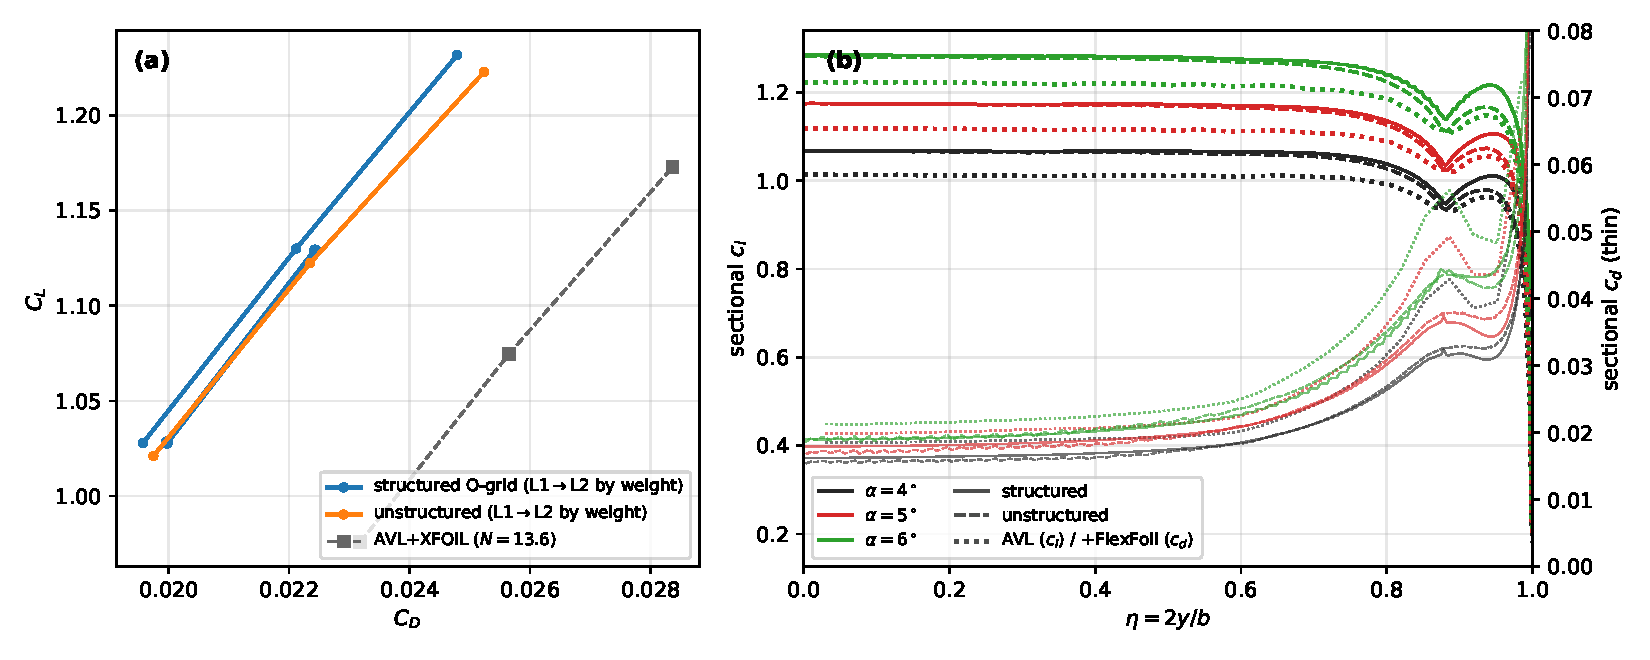
\includegraphics[width=0.99\textwidth]{daedalus_polar_sectional.pdf}
  \caption{The macroscopic comparison. \textbf{(a)} Wing polar: both
  mesh families at L1 and, where completed, L2 (color = family, line
  weight = level) against the AVL$+$XFOIL (vortex-lattice $+$ section
  polars) reference at matched $N_\mathrm{crit}$, trimmed to the RANS
  lift at each incidence (matched-lift reference). \textbf{(b)} Sectional lift on the finest
  grid with sectional output available per family and incidence
  against the AVL
  distribution (dotted), with sectional drag on the right axis (thin
  lines; the dotted reference is AVL induced drag, Trefftz-rescaled,
  plus the FlexFoil section profile drag): the loading agrees inboard
  to $\sim\!1\%$; the dip--recovery structure at the taper break
  ($\eta\!=\!0.88$) is mesh-family independent.}
  \label{fig:daepolar}
\end{figure}

The macroscopic ledger comes first (Fig.~\ref{fig:daepolar}; the
per-level coefficients are tabulated in Appendix~D,
Table~\ref{tab:daetotals}). The two families agree at L1 to
$0.6$--$0.8\%$ in $C_L$ and $0.9$--$1.8\%$ in $C_D$---and at
$\alpha\!=\!4^\circ$ and $5^\circ$, the incidences where both
finest grids are complete, to $0.6$--$0.7\%$ in $C_L$ and
$0.7$--$1.1$ counts ($0.35$--$0.5\%$) in $C_D$ at L2. Against the
AVL$+$XFOIL reference trimmed to the same total lift (the
lift-consistent comparison; the vortex lattice needs
$\sim\!0.5^\circ$ more incidence to carry the RANS $C_L$), the RANS
drag runs $13$ counts ($6.0\%$) low at $\alpha\!=\!4^\circ$,
$7$ ($3.1\%$) at $5^\circ$, and $2$ ($0.8\%$) at $6^\circ$ on the
finest grids---the deficit
shrinking with incidence, and entirely in the induced term's
territory, since the reference's profile drag barely moves with the
trim. (At matched \emph{incidence} the same reference sits $10$
counts lower still---the lattice carries $5\%$ less lift and hence
$\sim\!10\%$ less induced drag---which would flatter the RANS into
coincidence; the matched-lift numbers are the honest ones.)
The drag \emph{slope} disagrees more than the levels: mid-span
sectional drag grows at $\approx\!0.018$ per unit $c_l$ in the RANS
against the reference's $0.011$, all of whose growth is induced---the
strips' XFOIL profile drag is flat in lift, while the RANS profile
drag climbs $\approx\!6$ counts per $0.1$ of $c_l$. The sectional
diagnostic sheets of Appendix~D
(Figs.~\ref{fig:daesec10}--\ref{fig:daesec92}) locate the mechanism:
at fixed separation and reattachment---both match the strips at every
incidence---the model's handover-stretched pressure recovery inside
the bubble deepens with incidence, the $-C_p$ plateau persisting
further and recovering more gradually than the strip solution's
abrupt-closure recovery, and the area between the two curves growing
with $\alpha$: bubble pressure drag that an instant-transition
closure structurally cannot produce, the same mechanism as
Sec.~\ref{sec:epphandover} at the sections' $Re_c=5\times10^5$.
(The $\chi\!=\!1$ lead over $N\!=\!N_\mathrm{crit}$ holds its
$\sim\!0.09c$ convention offset at every incidence and contributes
no slope.) An accounting note for reading sectional comparisons
(\texttt{repro/cfd/daedalus\_strip\_accounting.py}): the RANS strip
curves reproduce their own force totals to a count, but the
reference's plotted sectional curve integrates a nearly
incidence-independent $18$--$21$ counts \emph{below} its own ledger
total---its induced shape is Trefftz-exact only in the integral, and
its profile term lives on nine FlexFoil stations that do not tile the
span---so sectional slopes are trustworthy where sectional level
differences are not.
At matched incidence the RANS lift runs $\sim\!5\%$ above the
lattice's---the excess a vortex lattice built on camber lines alone would
be expected to miss. A single-station decomposition makes it
quantitative: at $\eta\!=\!0.31$, $\alpha\!=\!4^\circ$
($\alpha_\mathrm{eff}\!\approx\!3.5^\circ$), the camber-only AVL
strip carries $c_l\!=\!1.011$, a thick-section inviscid panel solution
of the same DAE-11 gives $1.119$ ($+11\%$: thickness), viscous
FlexFoil at $N_\mathrm{crit}\!=\!13.6$ gives $1.053$ ($-6\%$:
decambering), and the RANS strip reads $1.066$---the wing's $5\%$
excess over the reference is the thin-airfoil truncation of the
vortex lattice, not a RANS surplus. Domain confinement does not explain the lift excess: the
two families' far fields differ by a factor of $\sim\!20$---the
O-grid's boundary is a cylinder of radius $100$ root chords,
$2.7$ spans for this wing, against the unstructured octree's
$\pm2$~km ($60$ spans)---yet their lifts agree to $0.7\%$. A
classical wall-interference estimate confirms the inference with room
to spare: treating the O-grid's outer boundary as a closed test section
of cross-section $C\!\approx\!4\!\times\!10^{4}$~m$^2$, the
upwash correction
$\Delta\alpha\!=\!\delta\,(S/C)\,C_L$ with
$\delta\!\approx\!0.12$ gives $\Delta C_L/C_L\!\sim\!0.06\%$
at these conditions---an order of magnitude below the families'
$0.7\%$ gap, which is therefore ordinary discretization difference,
not confinement. (Against the matched-lift reference the
predecessor-kernel campaign sat $15$--$26$ counts below; like-for-like
on each case, the final kernel's longer bubble---see below---returned
$6$--$14$ counts of bubble drag, leaving the $2$--$13$-count residual
above.) Sectional lift on the finest
grids with sectional output available
(Fig.~\ref{fig:daepolar}b) matches the vortex-lattice distribution
inboard to $\sim\!1\%$ and reproduces, identically on both families,
the dip--recovery structure at the taper break that the vortex lattice
smooths over.

\begin{figure}[p]
  \centering
  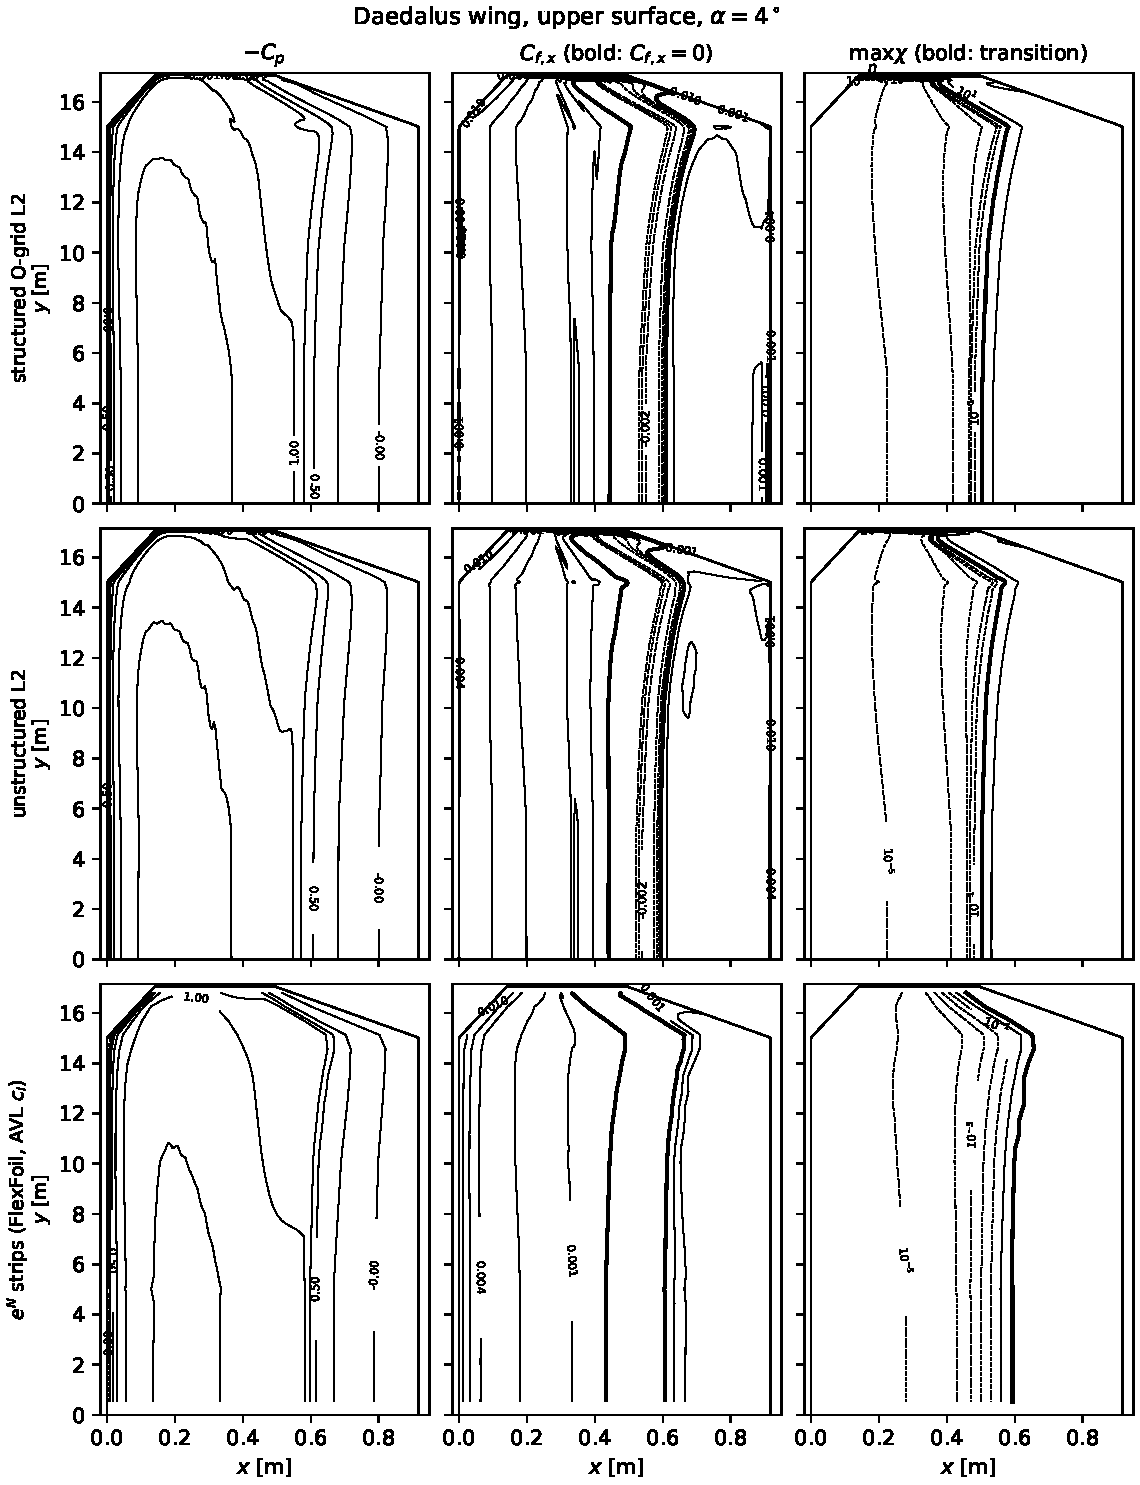
\includegraphics[width=0.99\textwidth]{daedalus_surface_a4.pdf}
  \caption{Daedalus wing upper surface at $\alpha\!=\!4^\circ$, finest
  completed grids, chord horizontal and span vertical (contour lines):
  $-C_p$ (left), streamwise skin friction $C_{f,x}$ (middle; the
  laminar separation bubble is bounded by the bold $C_{f,x}\!=\!0$
  contour), and the near-wall amplification $\max_n\chi$ in decade
  contours (right; bold: the model's transition front
  $\chi\!=\!1$). Rows: structured O-grid L2, unstructured L2, and the
  section-by-section $e^N$ reference---FlexFoil at each station's AVL
  $c_l$, local chord Reynolds number, and
  $N_\mathrm{crit}\!=\!13.6$, its $C_p$ from the Karman--Tsien-corrected
  edge velocity and its amplification drawn as $\chi_\infty e^{N}$ at
  the same decade levels (bold: $N\!=\!N_\mathrm{crit}$).}
  \label{fig:daesurf4}
\end{figure}

\begin{figure}[p]
  \centering
  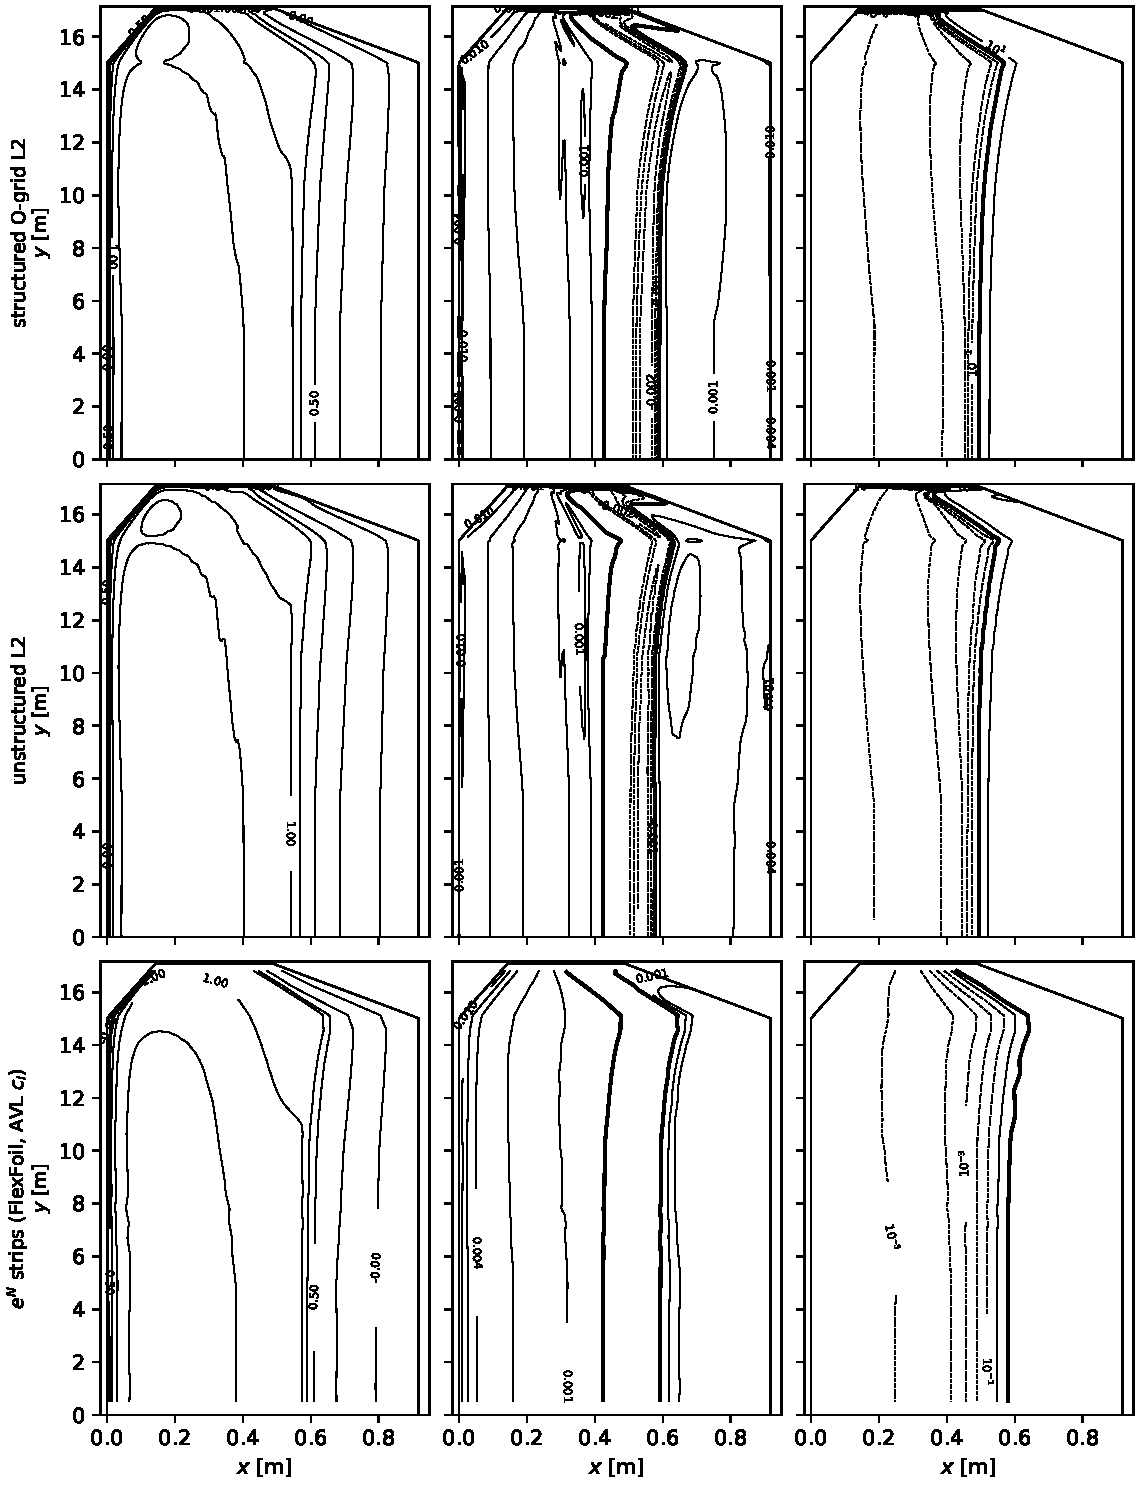
\includegraphics[width=0.99\textwidth]{daedalus_surface_a5.pdf}
  \caption{As Fig.~\ref{fig:daesurf4}, at $\alpha\!=\!5^\circ$ (the
  unstructured-L2 row will be added when that run's field output is
  regenerated).}
  \label{fig:daesurf5}
\end{figure}

\begin{figure}[p]
  \centering
  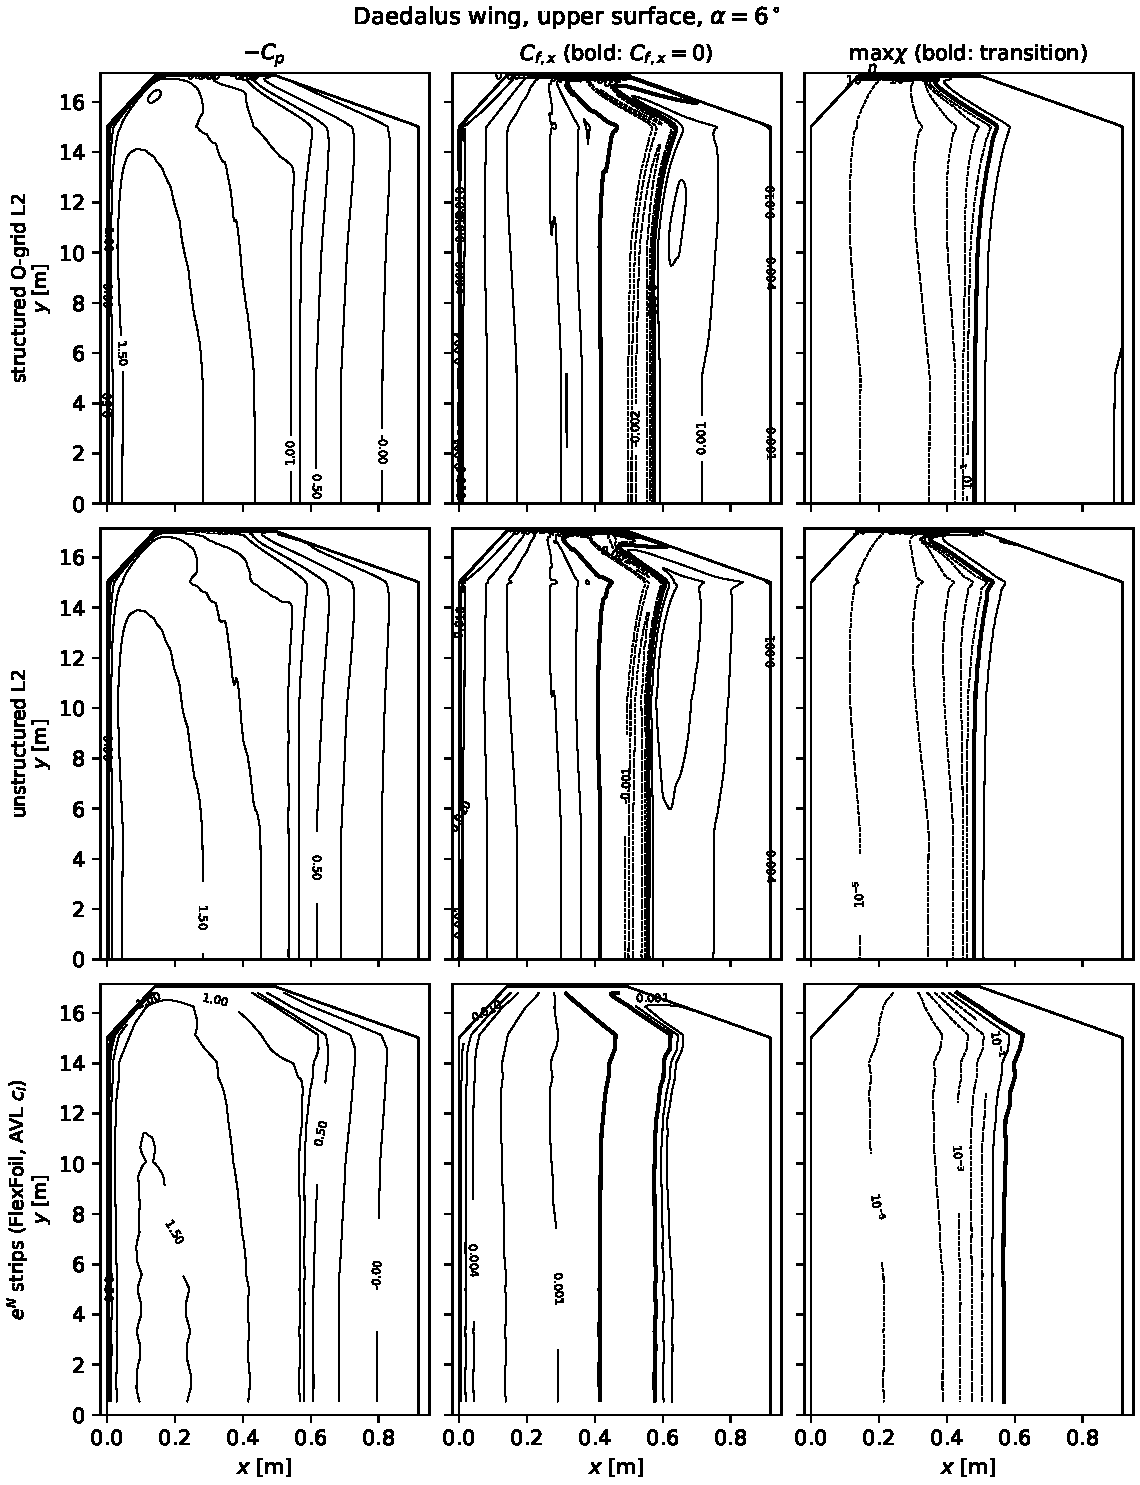
\includegraphics[width=0.99\textwidth]{daedalus_surface_a6.pdf}
  \caption{As Fig.~\ref{fig:daesurf4}, at $\alpha\!=\!6^\circ$ (the
  unstructured-L2 row will be added when that run completes).}
  \label{fig:daesurf6}
\end{figure}

The flow itself is read from the surface maps of
Figs.~\ref{fig:daesurf4}--\ref{fig:daesurf6}: the finest completed
RANS solution against the $e^N$ strips, column by column. The $-C_p$
maps
agree on the loading and carry the bubble's
pressure plateau at mid-chord. The $C_{f,x}$ maps carry the bubble
itself: a spanwise-uniform negative band whose extent now matches the
strips' station by station---at $\eta\!=\!0.31$,
$\alpha\!=\!4^\circ$ the RANS bubble spans $0.49$--$0.66\,c$ against
the strips' $0.47$--$0.66\,c$, at $5^\circ$ $0.47$--$0.65\,c$
against $0.47$--$0.65\,c$, and at $6^\circ$ $0.46$--$0.63\,c$
against $0.46$--$0.63\,c$: separation agrees to $0.02\,c$ and
reattachment to under $0.01\,c$ at every incidence. The reattachment is also the quantity
still moving under refinement---$0.63$ at L1 to $0.66$ at L2 against
the strips' $0.66$---while separation and the $\chi$ field are
level-converged, and the two families agree to $0.02\,c$ on
both edges---at L1 at every incidence, and at L2 at $4^\circ$
(fronts $0.002\,c$ apart, separation $0.008$, reattachment
$0.016\,c$). The $\chi$ maps show the interior anatomy: the bubble's
\emph{extent} matches the strips' station by station, but the model's
transition front ($\chi\!=\!1$, bold in the figure) sits near
mid-bubble, $\sim\!0.09\,c$ ahead of the strips' $N_\mathrm{crit}$
contour, which sits just ahead of reattachment. At this chord Reynolds
number the early front is the seed convention, not the low-$Re$ defect
pair of Sec.~\ref{sec:epphandover} (whose re-seeding measurement is
quiet at these $Re$): $\chi\!=\!1$ sits
$\ln(1/\chi_\infty)\!=\!11.7$ $e$-folds up the same envelope
against the strips' $N_\mathrm{crit}\!=\!13.6$, and the in-bubble
envelope climbs $\sim\!2$ $e$-folds per $0.09\,c$. What the wing
does share with Sec.~\ref{sec:epphandover} is the commit half: the
model spends the remainder of the bubble bringing the eddy viscosity
to closing strength where the $e^N$ reference commits at once---both
halves short enough here that the sum, separation to reattachment,
lands on the reference.

This bubble length is the final kernel's correction at work: the
predecessor-kernel campaign on the same grids returned the same
fronts---its $\chi\!=\!1$ contour sat the same $\sim\!0.1\,c$
ahead of the strips' $N_\mathrm{crit}$ contour---but closed the bubble
three to four times sooner ($0.04$--$0.06\,c$). That kernel applied the free-shear ceiling from
the separation point on, while a just-separated layer is still
wall-damped---its instability approaches the free-shear rate only as
it lifts several $\theta$ off the surface---and, as the frozen-profile
ledger of Appendix~D measures in temporal units, its transported
$\tilde\nu$ peak rode below the physical critical layer at roughly
half its convection speed, banking nearly twice the $e$-folds per unit
length (an excess intrinsic to a temporal rate advected by the local
velocity, \S\ref{sec:reproduce}). The in-bubble arm of the final
onset threshold (the $B/\langle\hat\Omega \hat I\rangle_+^{2}$ branch of
Eq.~\eqref{eq:reomc}, which suppresses the rate while the separated
layer is still wall-damped) was built to
close exactly this blind spot, and the recomputation confirms it
does: the wing bubble lengthened from $0.04$--$0.06\,c$ to the
strips' $\sim\!0.2\,c$, and the $6$--$14$ counts of bubble drag that
the predecessor was missing returned to the polar.

Two spanwise phenomena, invisible to any sectional diagnostic, close
the study; both are read directly off the maps of
Figs.~\ref{fig:daesurf4}--\ref{fig:daesurf6}. Outboard of the taper
break the falling chord Reynolds number stretches the bubble toward
the trailing edge---at $\alpha\!=\!4^\circ$ its reattachment retreats
from $0.66\,c$ at $\eta\!=\!0.31$ to $0.79\,c$ at $\eta\!=\!0.92$ and
$0.95\,c$ at $\eta\!=\!0.97$, mirroring the strips'
$0.66\!\to\!0.74\!\to\!0.84$, the $C_{f,x}$ bands bending aft in
unison. And over the last half-percent of span the tip vortex trips
the boundary layer, pulling transition to the leading edge in a
compact patch at the tip ($\chi$ exceeds unity from the leading edge
for $\eta\!\gtrsim\!0.995$; the bright sliver at the top of the RANS
$\chi$ maps): a genuinely three-dimensional transition mechanism,
captured by the transported amplification with no special
treatment---and absent, necessarily, from the sectional $e^N$ row.

\section{Toward crossflow: the 6:1 prolate spheroid}\label{sec:spheroid}

The inclined 6:1 prolate spheroid is the canonical fully
three-dimensional transition benchmark: the DFVLR campaign of Kreplin,
Vollmers, and Meier~\cite{kreplin_1985} mapped the wall shear stress
(magnitude and direction) over the whole body with surface hot films,
and the transition-modeling literature validates against it in a
standard presentation---the surface unrolled into the
$(x/L,\phi)$ plane ($\phi\!=\!0$ the windward symmetry line), with
skin-friction magnitude, wall-shear direction, and the transition
front drawn as maps. The definitive stability analysis of the case
is Stock's~\cite{stock_2006}: transition is pure-TS at low
incidence, mixed TS--crossflow at $\alpha\!\approx\!5$--$15^\circ$
and $Re_L\!\gtrsim\!6.5\!\times\!10^6$, pure-crossflow beyond---and
at $Re_L\!=\!1.5\!\times\!10^6$ the boundary layer stays laminar up
to the open free-vortex-layer separation, with the measured fronts
tracking the separation line itself. Figure~\ref{fig:spheroidmaps} shows SA-AI in
exactly this presentation: the analytic spheroid
($x^2\!/A^2+r^2\!/B^2\!=\!1$, $A\!=\!L/2$, $B\!=\!L/12$, half-model)
on a structured O-grid ladder (L0--L2:
$0.37$/$2.2$/$12.6$ million nodes, first wall spacing halving per
level from $5\!\times\!10^{-6}L$), at $Re_L\!=\!1.5\!\times\!10^6$,
$M\!=\!0.1$, $\alpha\!=\!10^\circ$, with the airfoil-study solver
settings, seed, and constants unchanged. All three levels are
computed; the figure shows L1, and the level-to-level totals are not
yet grid-converged ($C_L\!=\!0.205/0.208/0.186$ over L0/L1/L2), so
the finest-level map comparison accompanies the front overlays. The model carries no
crossflow closure---the amplification rate is calibrated on
two-dimensional TS growth---so this case probes what that economy
costs on a crossflow-dominated body; the maps here are the
infrastructure for that comparison, with the measured-front overlays
and the workshop condition ($Re_L\!=\!6.5\!\times\!10^6$) to follow.
Figure~\ref{fig:spheroid3d} shows the same skin friction on the body.

\begin{figure}[tp]
  \centering
  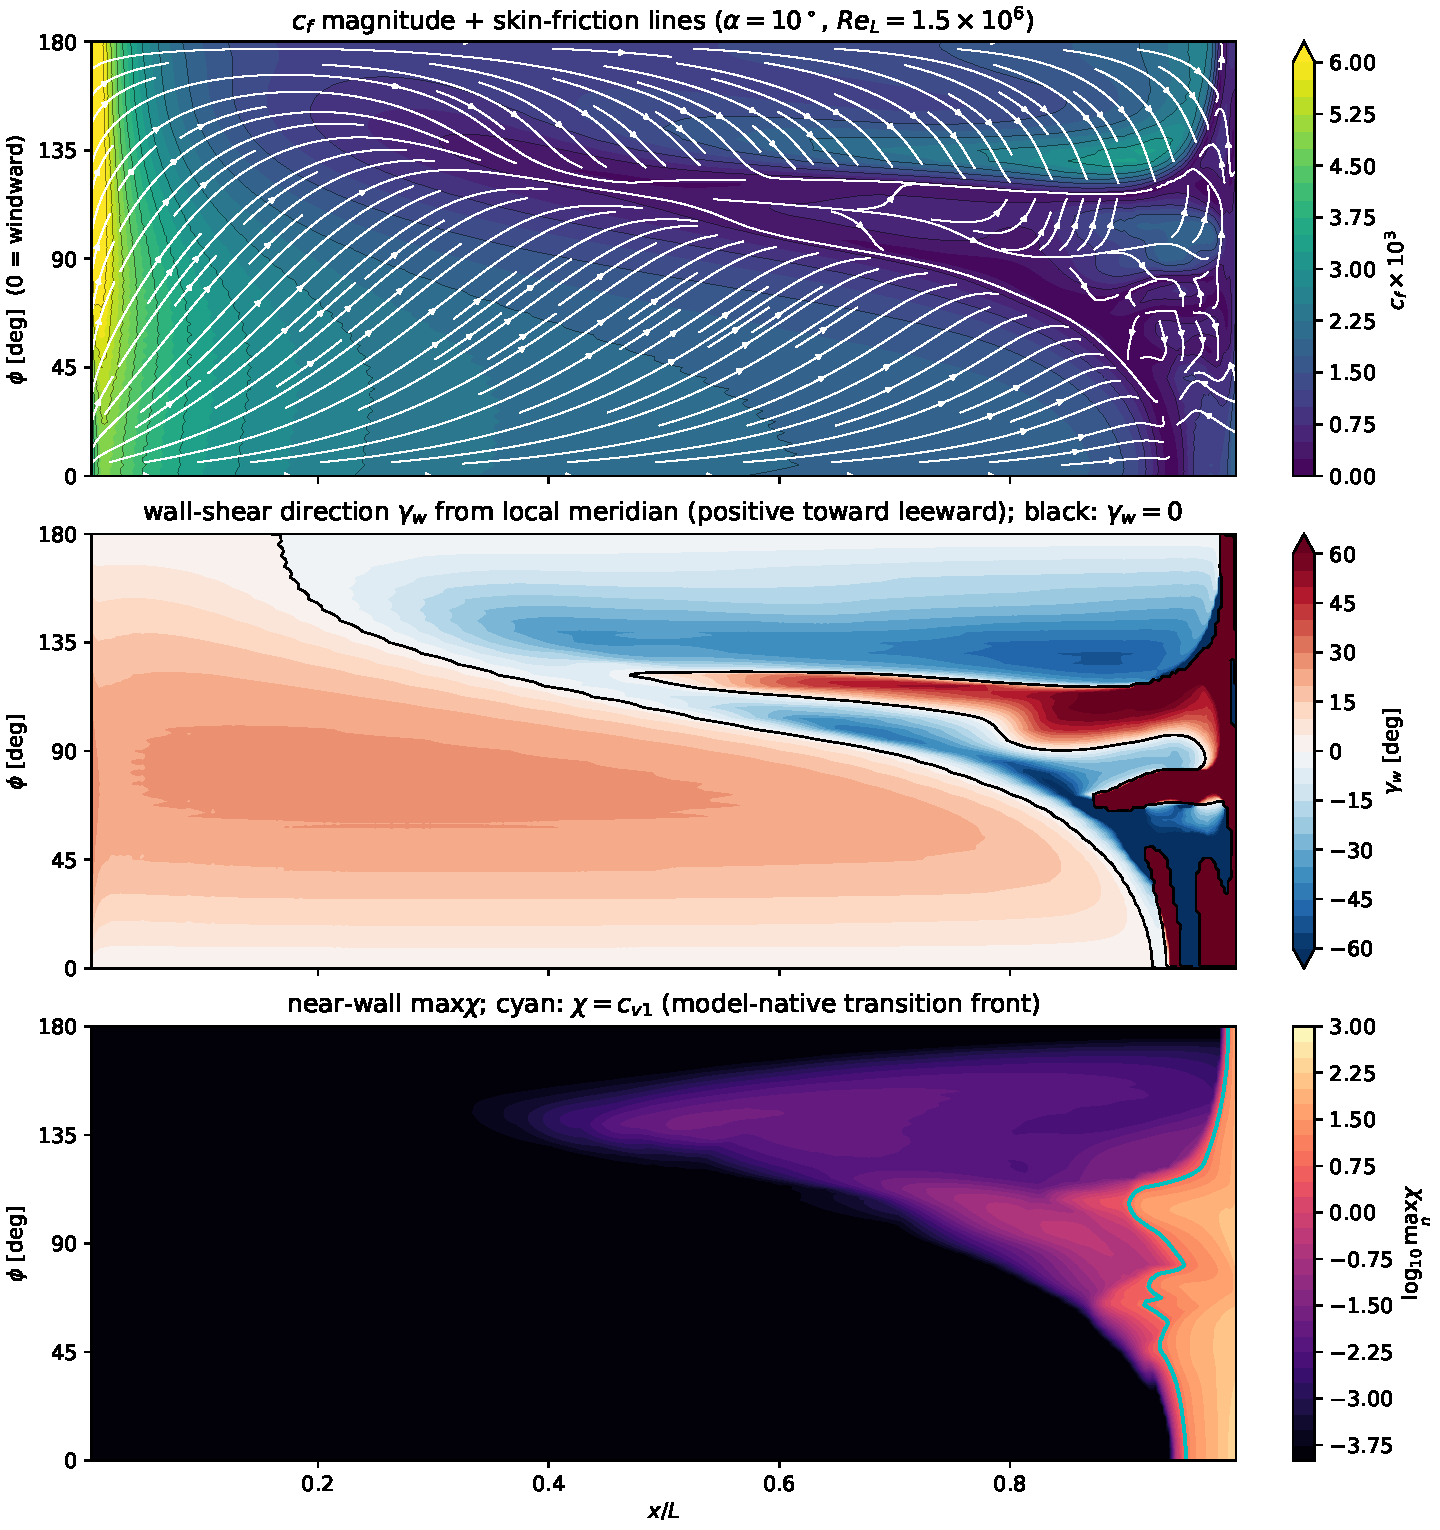
\includegraphics[width=0.99\textwidth]{spheroid_maps_L1.pdf}
  \caption{6:1 prolate spheroid, $Re_L\!=\!1.5\!\times\!10^6$,
  $\alpha\!=\!10^\circ$, SA-AI on the L1 O-grid ($2.2$M nodes),
  surface unrolled into $(x/L,\phi)$, windward line at
  $\phi\!=\!0$. Top: $c_f$ magnitude with skin-friction lines (the
  oil-flow analogue); the friction lines converge onto the leeward
  separation-line band at $\phi\!\approx\!100$--$135^\circ$. Middle:
  wall-shear direction $\gamma_w$ from the local meridian (positive
  toward leeward), the quantity the DFVLR hot films
  measured~\cite{kreplin_1985}; the black $\gamma_w\!=\!0$ line marks
  the crossflow reversal under the leeward vortex. Bottom: wall-normal
  maximum of $\chi$ with the $\chi\!=\!c_{v1}$ contour (cyan) as the
  model-native transition front: at this Reynolds number the body runs
  laminar to $x/L\!\approx\!0.9$ on the windward side, with
  amplification building (but not committing) under the leeward
  vortex from mid-body.}
  \label{fig:spheroidmaps}
\end{figure}

\begin{figure}[tp]
  \centering
  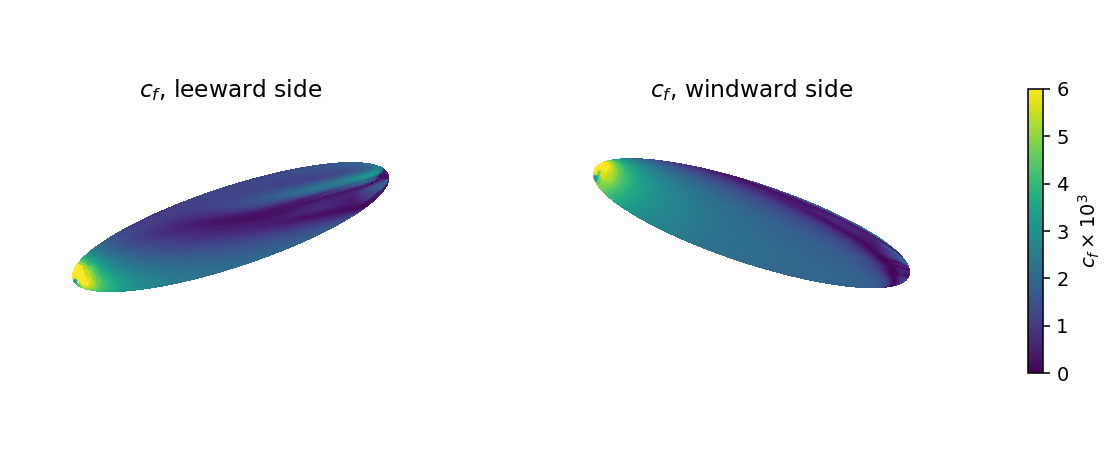
\includegraphics[width=0.9\textwidth]{spheroid_maps_L1_3d.png}
  \caption{The $c_f$ magnitude of Fig.~\ref{fig:spheroidmaps} rendered
  on the body (leeward and windward views), the presentation of the
  N-factor and skin-friction contour figures of the
  transition-prediction literature on this case.}
  \label{fig:spheroid3d}
\end{figure}

\section{Conclusion}

The Spalart--Allmaras working variable can, it turns out, serve as its
own transition indicator. By replacing the production in the laminar range with a local,
$e^N$-like amplification rate and reverting to standard SA near
$\chi\!\sim\!1$, a single transport equation predicts natural transition
without any auxiliary field.

The amplification rate is anchored to canonical stability limits, not to the
transition cases. Its ceiling $a_{\max}\!=\!0.19$ is the tanh free-shear
(Kelvin--Helmholtz) eigenvalue, reached undiluted at the vorticity pole; its
geometry---the vorticity fraction $\hat\Omega$ and the accumulated-inflection
coordinate $\hat I$, whose
even product $\hat\Omega\hat I$ is the single amplifying coordinate the projective
algebra allows---is fixed by the mean profile alone; and its viscous onset is a
gate on the vorticity Reynolds number whose threshold $Re_\Omega^{\mathrm c}(\hat\Omega \hat I)$
takes its shape from linear stability theory and its single free scale from
the $N\!=\!1$ crossing of the Blasius $e^N$ envelope alone---the $N\!=\!9$
crossing is then an untuned prediction, landing $7\%$ past Drela's---the
residual footprint of the retained laminar diffusion. A favorable gradient keeps the curvature single-signed, so
$\hat\Omega \hat I\!\to\!0$ and the rate extinguishes geometrically, with no pressure-gradient
parameter. The model was then exercised across three pressure-gradient regimes. The freestream-turbulence
closure $\chi_\infty(Tu)$ is Mack's $e^N$ correlation, and the destruction-gate
weight is tied to the production weight by a wall-layer identity, so the
linear $\tilde\nu$ wall solution---and with it the log law---is exactly
standard SA's. On a zero-pressure-gradient flat plate (Sec.~\ref{sec:flatplate}) the Mack
closure places transition onset (at the stated half-saturation
$\chi\!=\!c_{v1}$ convention,
$Re_\theta$ integrated from the computed profiles)
within $10\%$ of the Abu-Ghannam \& Shaw
correlation over the natural-transition range ($7\%$ late at the lowest
disturbance level---the retained-drain footprint---within $2\%$ at
$Tu\!=\!0.08\%$, and $4$--$10\%$ early above),
verifying the Blasius envelope. On
the NLF(1)-0416 at $Re\!=\!4\!\times\!10^6$ (Sec.~\ref{sec:nlfval}) the
model holds the designed laminar rooftop---the favorable run held by
$\hat\Omega \hat I\!\to\!0$ with no pressure-gradient term---and ignites at each recovery,
tracking the Somers fronts (the lower front's aft-ward march with lift
reproduced to within $0.02\,c$), and the
handover held across $\alpha\!\in\!\{0^\circ,4^\circ,9^\circ,15^\circ\}$ on
twenty-four cases (both mesh families, three refinement levels), plus the
finest-grid negative pair. On the Eppler
387 at
$Re\!=\!2\!\times\!10^5$ (Sec.~\ref{sec:eppval}) the
model resolved the adverse-gradient, laminar-separation-bubble regime---the signed
skin friction shows the recirculation directly---across another thirty-six cases
on the same two-family ladder (twelve of them the finest-pair extension over
$\alpha\!=\!-2^\circ$--$8.5^\circ$), though it reattaches late at low
incidence---$0.02$--$0.04\,c$ aft of the measured oil-flow reattachment at
$\alpha\!\le\!5^\circ$ ($0.76$ vs $0.74\,c$, $0.71$ vs $0.67\,c$, $0.63$ vs
$0.59\,c$, inside the facility-to-facility spread of the two
experiments on Fig.~\ref{fig:eppbubble}), and early at $7^\circ$
(\S\ref{sec:calib_rate}); an $\alpha\!=\!5^\circ$ sweep across five Reynolds numbers,
$Re\!=\!6\!\times\!10^4$ to $4.6\!\times\!10^5$, follows the bubble's march and
shortening. The same constants (Appendix~E) were used
throughout. Across both airfoils the L1$\to$L2 transition-location drift is at
or below $0.01\,c$ (reaching $0.008\,c$ at the NLF's near-LE
$\alpha\!=\!9^\circ$ front and $0.011\,c$ on the Eppler
reattachment), and the two independently-generated mesh families
agree to within $0.02\,c$ of chord on every transition front and to
$0.004$--$0.011\,c$ on the Eppler reattachment at L2 (the
edge-of-collapse $7^\circ$ case excepted, where three grids retain
no bubble). The Reynolds sweep
also locates the model's low-$Re$ boundary: the Eppler bubble fails to
close at $10^5$ on every grid, and an exhaustive initialization study
(cold starts, Reynolds-number forks, slow continuation in both
directions, each endpoint extended to convergence) shows the computed
state is \emph{unique} at every swept Reynolds number---the model
places its bursting boundary one Reynolds step above the measurement
and carries no counterpart of the two-state structure the experiment
shows at $6\!\times\!10^4$---traced quantitatively to the length of the
deliberately unmodeled transition zone, which at these Reynolds numbers
grows to a macroscopic fraction of the chord and starves the bubble of
eddy viscosity---and to a second, opposite-signed defect it partially
cancels against, the closed-cell re-seeding of the amplification by
$\tilde\nu$ recirculating under the bubble's shear layer; low-$Re$
bubbles the model gets right are the sum of these canceling errors
(Sec.~\ref{sec:epphandover}). In three dimensions, on
the Daedalus wing at flight conditions, the completed runs of the
final-kernel campaign put the mid-span bubble's separation within
$0.02\,c$ and its reattachment within $0.01\,c$ of the strip-theory
$e^N$ reference, and capture two spanwise mechanisms no sectional
method sees---the outboard bubble stretch past the taper break and the
tip-vortex trip (Sec.~\ref{sec:daedalus}).

Several extensions follow. The clearest limitation is the linear rate's
under-amplification of strongly favorable and strongly separated profiles---the
favorable envelope of Fig.~\ref{fig:calibrate} and the over-long Eppler bubble
both trace to it---so a shaped rate that restores the near-neutral floor without
a pressure-gradient parameter is the natural refinement. The second is
the transition zone itself: an outer-scaled, memory-carrying closure
for
$\sigma_t$---a spot-growth or intermittency treatment replacing the
memoryless fixed-$\chi$-width interpolation, whose narrowing alone only
trades the bias for a relaxation oscillation---would move
the bursting boundary toward the measured one
(Sec.~\ref{sec:epphandover}). A calibration against
linear-stability and $e^N$ databases beyond the anchors used here---and a
direct comparison with the algebraic SA-BCM model on community-standard
benchmarks---would establish accuracy beyond the present demonstration.
The out-of-scope regimes noted in the introduction---bypass, crossflow, and
compressible transition---are the natural next steps. For crossflow
specifically, the Gram algebra of Eq.~\eqref{eq:gram} already
contains the natural sensor: the odd pairing
$\langle\nabla d,\,\mathbf u\times(\boldsymbol\omega\times\mathbf d)\rangle$,
equal, for wall-parallel vorticity, to the helicity density times
the layer depth, vanishing
identically in two-dimensional flow, and measuring exactly the
crossed shear a swept boundary layer adds---a second amplification
channel in the same local language.

\begin{center}
  \begin{minipage}{0.6\textwidth}\centering
  \begin{CJK}{UTF8}{bsmi}天下萬物生於有，有生於無。\end{CJK}\\[3pt]
  \emph{The myriad things are born of being;\\
  being is born of non-being.}\\[3pt]
  ---\emph{Daodejing}, ch.~40
  \end{minipage}
\end{center}

\section*{Acknowledgments}
The initial idea for this approach was sparked by conversations with Mark Drela
and Philippe R.\ Spalart, whose insights on the amplification-factor envelope
and on the structure of the SA equation were formative.

\bibliography{references}

\clearpage
\appendix
\renewcommand{\thefigure}{A\arabic{figure}}
\setcounter{figure}{0}
\section*{Appendix A: the NLF(1)-0416---meshes and wall-anchored
contour sheets}

Each of the following appendices collects, for one main-text section,
the mesh views and the wall-anchored contour sheets of its cases:
Appendix~A for the NLF(1)-0416 study (Sec.~\ref{sec:nlfval}),
Appendix~B for the Eppler~387 benchmark (Sec.~\ref{sec:eppval}),
Appendix~C for the Eppler Reynolds sweep (Sec.~\ref{sec:eppresweep}),
and Appendix~D for the Daedalus wing (Sec.~\ref{sec:daedalus}).

Figures~\ref{fig:nlfmesh_str} and~\ref{fig:nlfmesh_cav} show the
leading- and trailing-edge close-ups of the structured O-grid and
unstructured cavity families at the three refinement levels. The
cavity mesher is driven by the anisotropic metric
\begin{equation*}
  \mathsf M(\mathbf x)=R\,\mathrm{diag}\!\left(h_n^{-2},\,h_t^{-2}\right)R^{\mathsf T},
  \qquad
  h_n=\min\!\big(h_0+(\gamma-1)\,d,\;h_\infty\big),
  \quad
  h_t=\min\!\big(h_w+(\gamma-1)\,d,\;h_\infty\big),
\end{equation*}
where $d$ is the distance to the nearest wall point, $R$ rotates into
the (wall-normal, wall-tangential) frame of that nearest point,
$h_0$ is the first-cell height of
Tables~\ref{tab:nlfmesh}/\ref{tab:eppmesh}, $\gamma$ the growth
ratio, $h_w$ the wall-tangential metric input, and $h_\infty$ the
isotropic far-field size; per level L0/L1/L2 the inputs are
$\gamma\!=\!1.2/1.1/1.05$, $h_w\!=\!0.008/0.004/0.002$, and
$h_\infty\!=\!3.0/2.0/1.5$ (chords). The metric governs the
interior only---the boundary spacing comes from the resampled
contour---and $h_\infty$, unlike every near-wall scale, does not
halve per level (it is reached only far outside the region the
sheets and tables measure).

Wherever a five-row figure's dotted or dash-dotted reference $C_f$
comes from an XFOIL or FlexFoil surface dump (the mfoil references
are already freestream-normalized), it is converted from the dumps'
edge normalization to the freestream convention of the computed rows
($\times u_e^2$).

The contour sheets present the computed fields in the manner of the
flat-plate figure (Fig.~\ref{fig:flatplate_batch}): line contours of
the velocity magnitude $|\mathbf{u}|/U_\infty$ (left column) and of
$\log_{10}\chi$ (right column; dashed contours are the laminar levels
$\chi<1$, solid are $\chi\!=\!1$, $c_{v1}$, $30$, and $10^2$---the
last two tracking the handover's completion and the turbulent
interior), on wall-anchored
coordinates---the abscissa is the $x/c$ of the wall anchor, the
ordinate the wall-normal distance from that anchor, so each wall-normal
probe scan is one vertical line of the panel. Rows pair the two mesh
families at each refinement level (cavity, then O-grid; L0, L1, L2).
The wall-normal range is chosen to hold the laminar band in frame
($0.0015c$ upper and $0.0025c$ lower for the NLF(1)-0416, scaled with
$1/\sqrt{Re}$ for the other cases), letting the turbulent layer
overshoot the frame top---except the Eppler upper surface, whose frame
is raised a further $5\times$ ($0.0335c$ at $2\times10^5$) so the
handover above the lifted bubble shear layer stays in frame.

\begin{figure}[p]
  \centering
  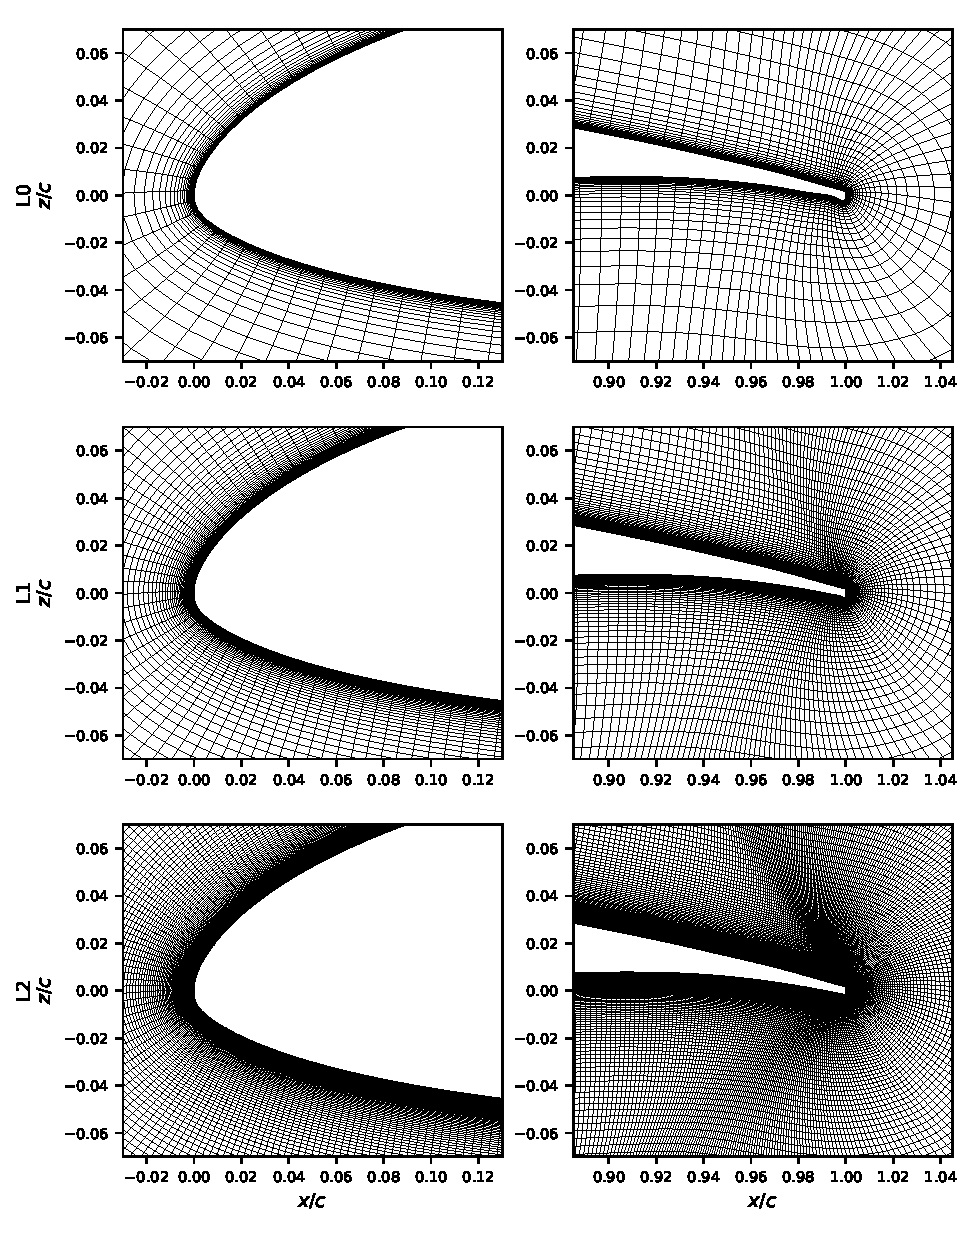
\includegraphics[width=\textwidth,height=0.92\textheight,keepaspectratio]{mesh_nlf_str.pdf}
  \caption{NLF(1)-0416 structured O-grid mesh at the leading edge (left column)
  and blunt trailing edge (right column) for the three refinement levels
  L0--L2 (rows). The O-grid wraps the section with wall-normal clustering for
  the boundary layer; every length scale halves per level. Chord normalized to
  unity ($z$ vertical).}
  \label{fig:nlfmesh_str}
\end{figure}

\begin{figure}[p]
  \centering
  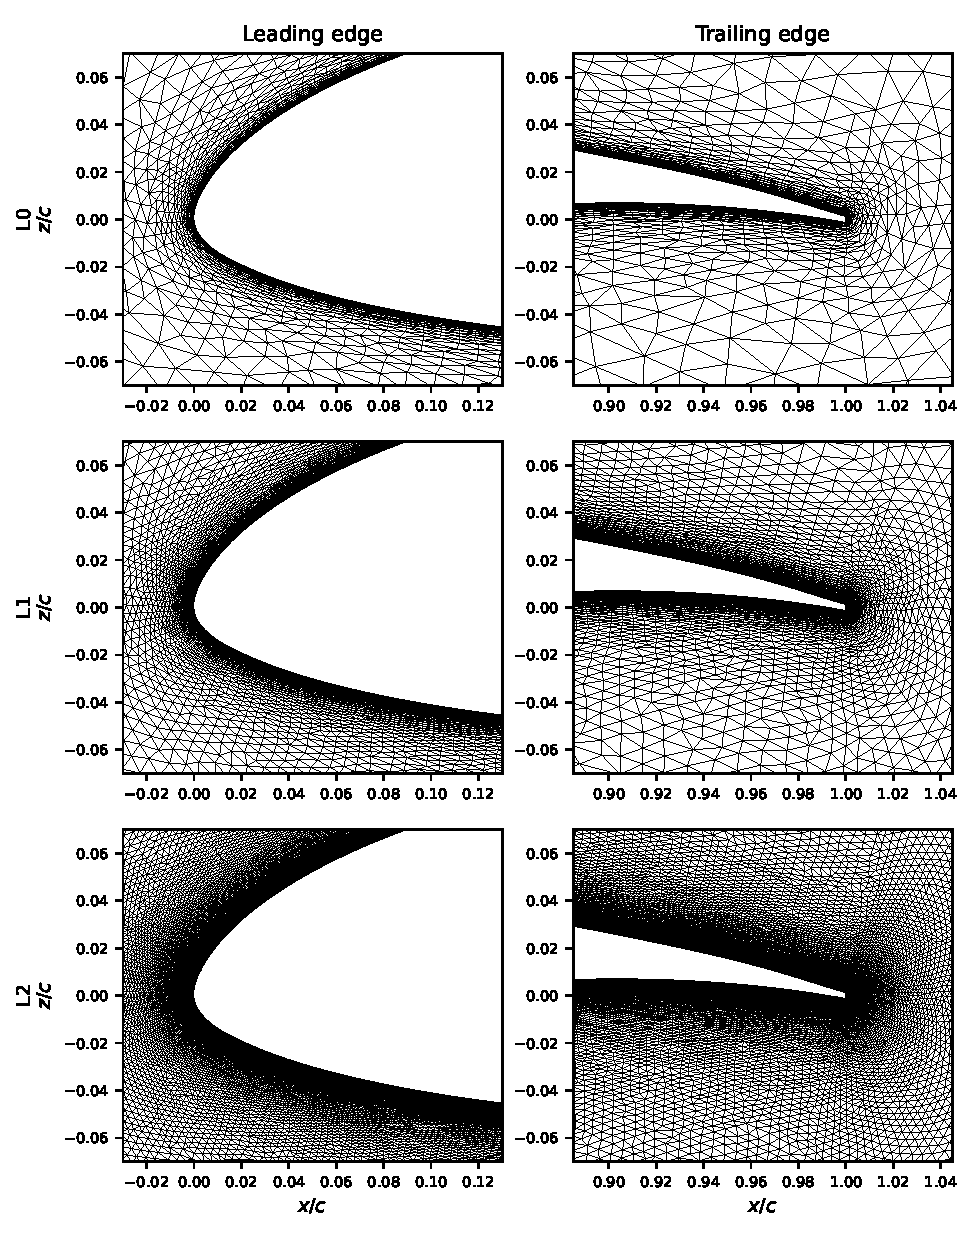
\includegraphics[width=\textwidth,height=0.92\textheight,keepaspectratio]{mesh_nlf_cav.pdf}
  \caption{NLF(1)-0416 unstructured cavity mesh (leading and trailing edges,
  levels L0--L2), built from the same arc-length cubic-spline contour as the structured grid of
  Fig.~\ref{fig:nlfmesh_str} with blunt-trailing-edge--aware spacing. Every
  length scale halves per level.}
  \label{fig:nlfmesh_cav}
\end{figure}

\begin{figure}[p]
  \centering
  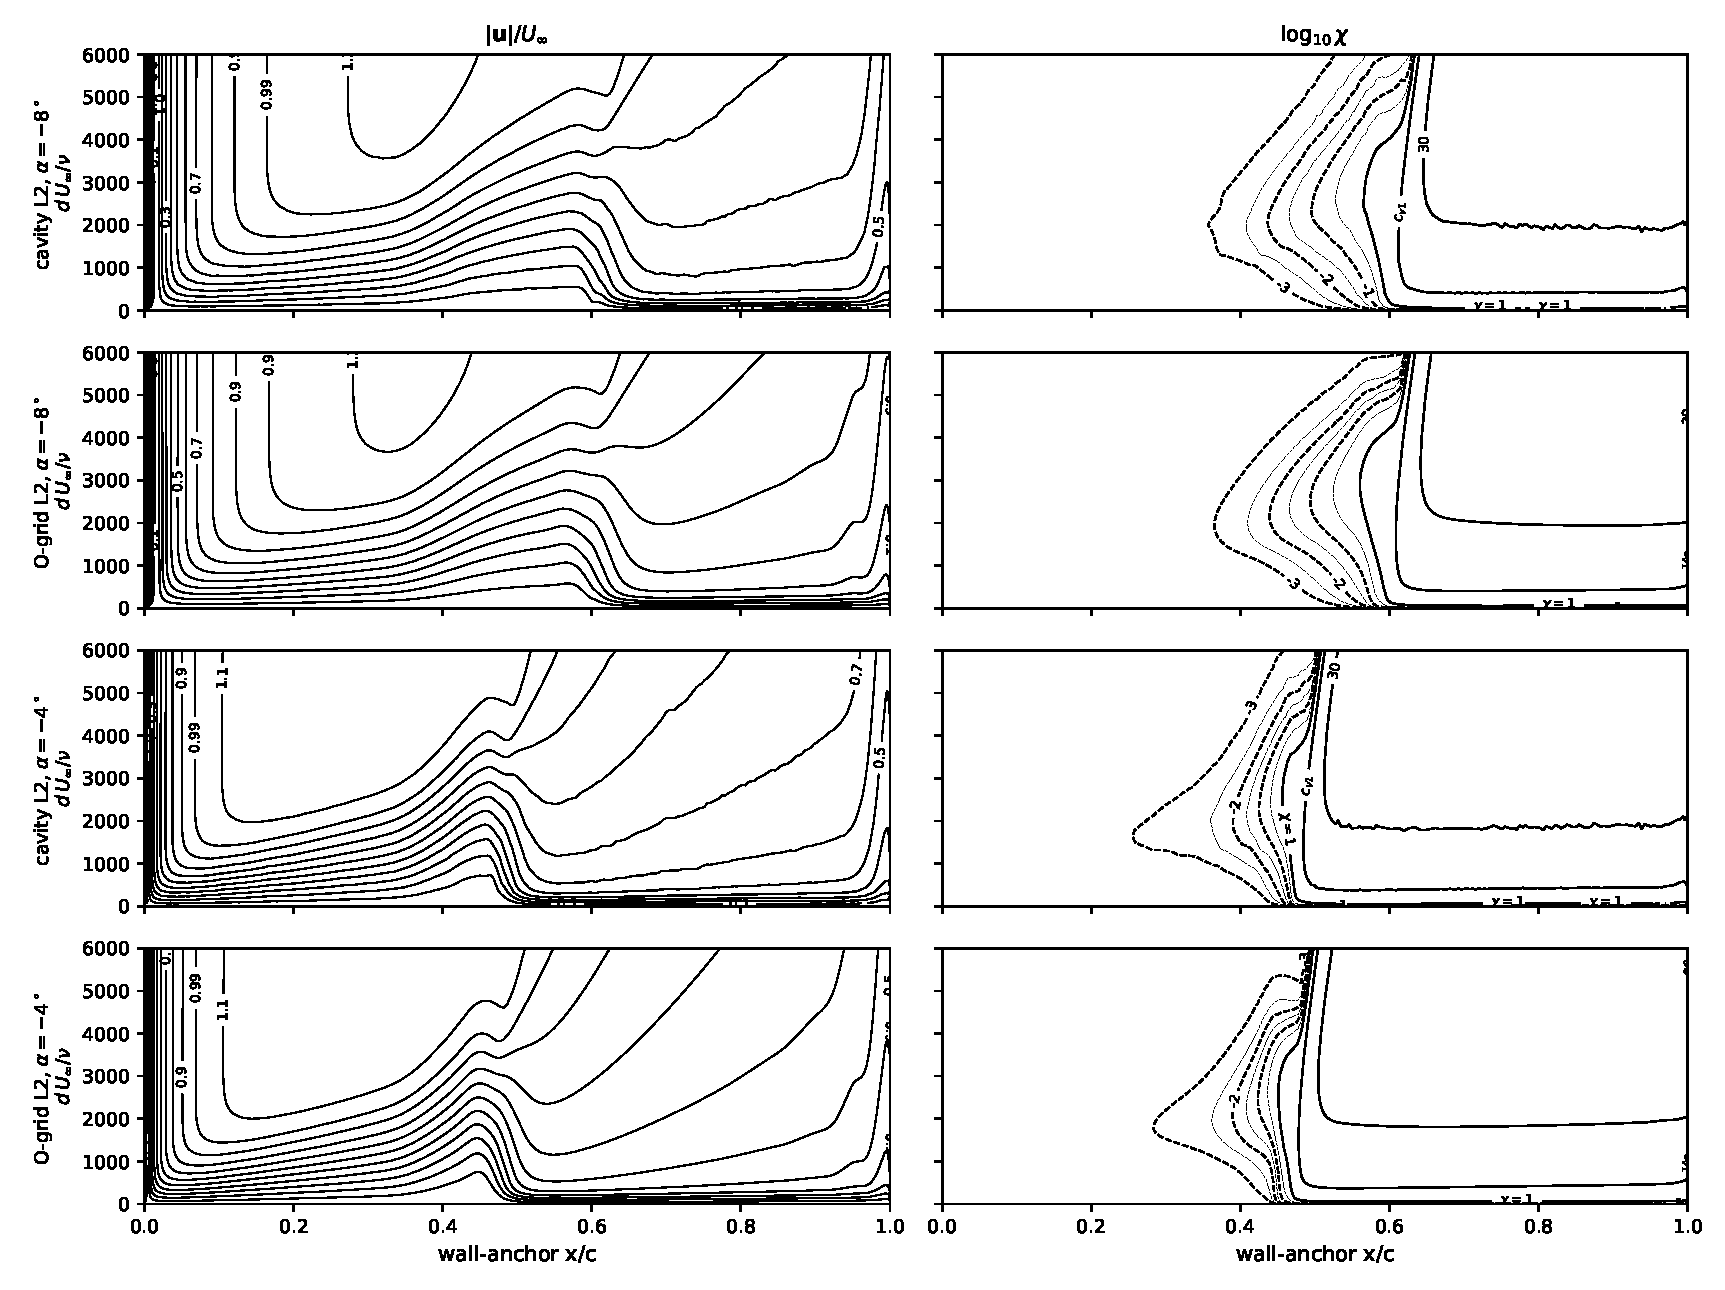
\includegraphics[width=0.99\textwidth]{chi_sheet_nlf0416_negalpha_upper.pdf}
  \caption{NLF(1)-0416 negative-incidence pair, upper surface: rows are
  (cavity, O-grid) L2 at $\alpha=-8^\circ$ then $-4^\circ$. At
  $-8^\circ$ this (pressure) surface holds a long laminar run before
  its front settles at $0.56\,c$ (Fig.~\ref{fig:nlfnegalpha}).}
  \label{fig:sheet_nlf0416_negalpha_upper}
\end{figure}

\begin{figure}[p]
  \centering
  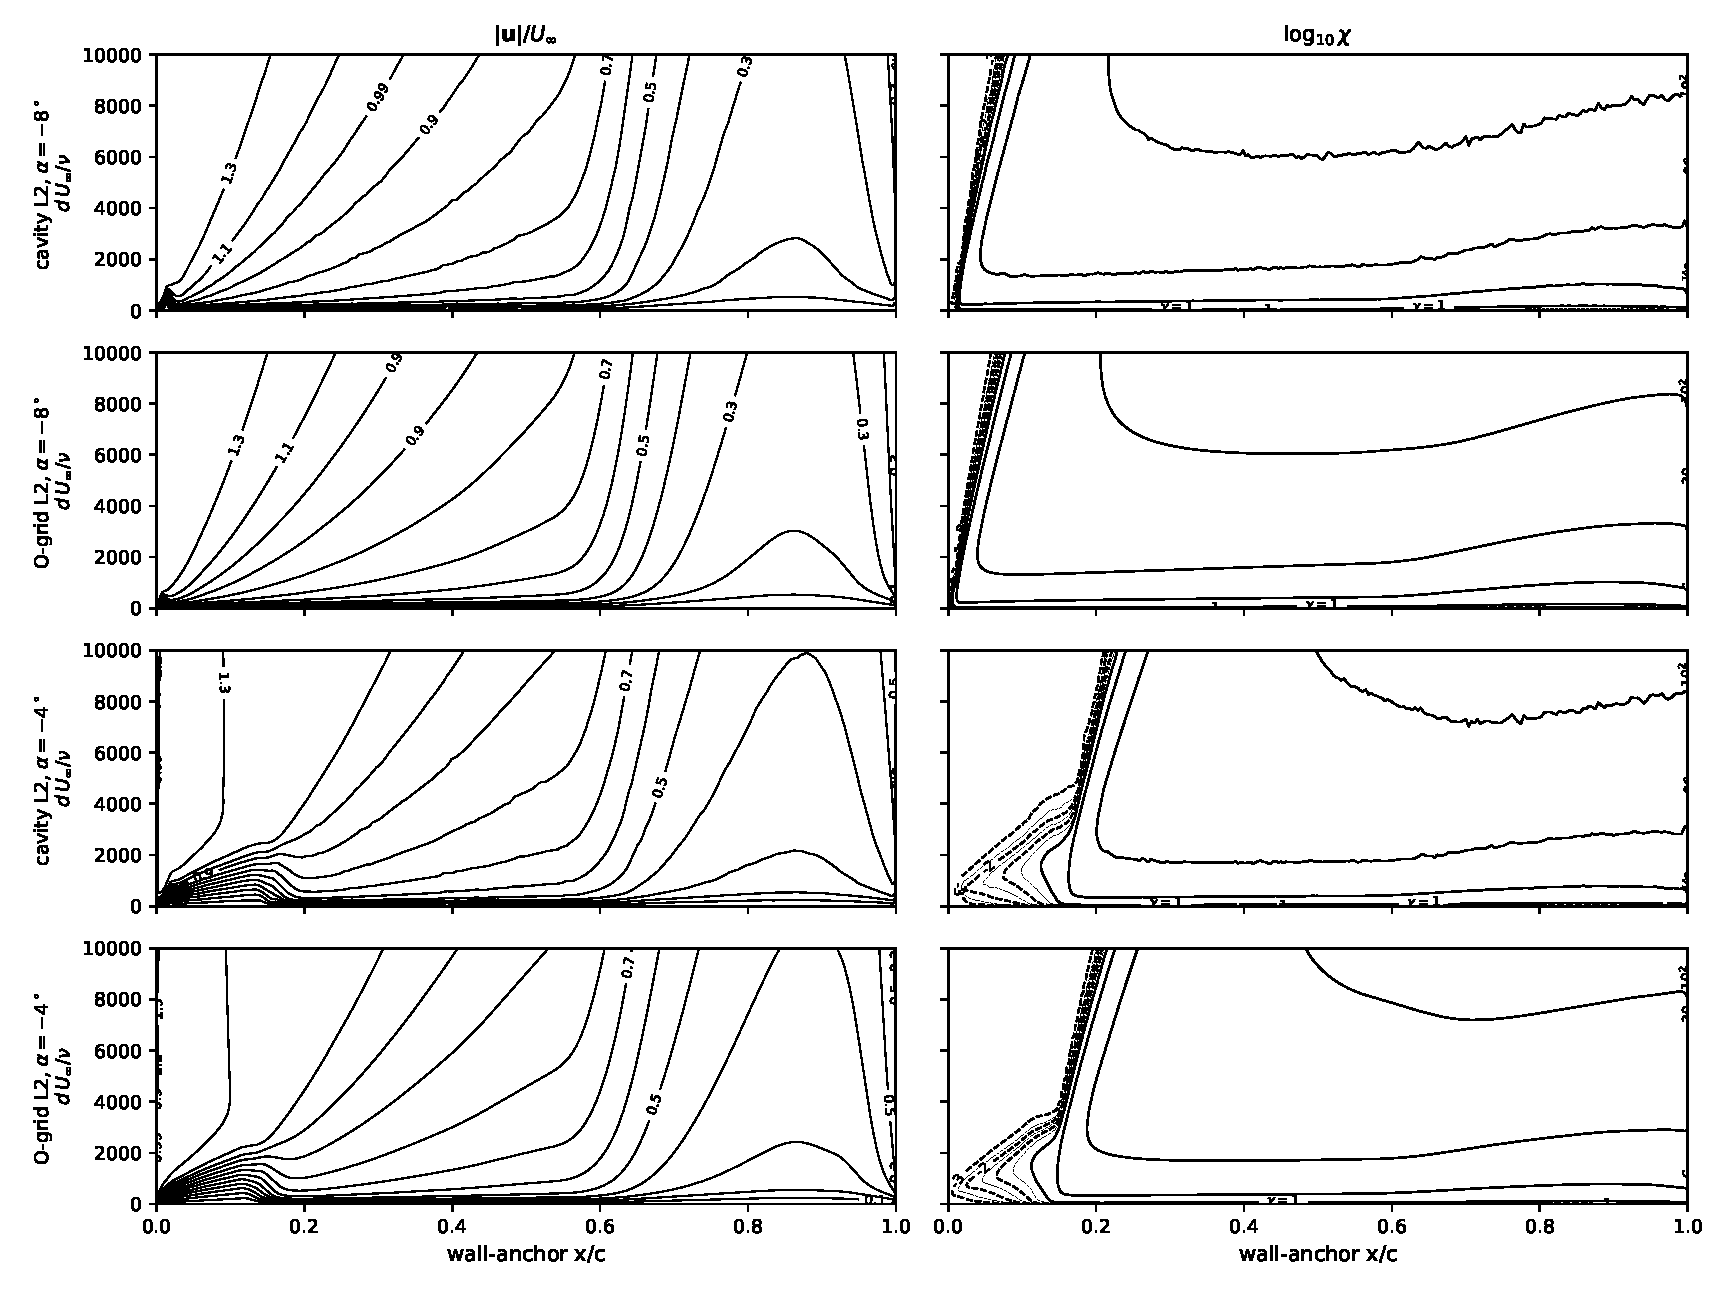
\includegraphics[width=0.99\textwidth]{chi_sheet_nlf0416_negalpha_lower.pdf}
  \caption{As Fig.~\ref{fig:sheet_nlf0416_negalpha_upper}, lower
  surface: tripped at the leading edge at $-8^\circ$ (the suction side
  there) and laminar to ${\approx}0.11$--$0.12\,c$ at $-4^\circ$.}
  \label{fig:sheet_nlf0416_negalpha_lower}
\end{figure}

\begin{figure}[p]
  \centering
  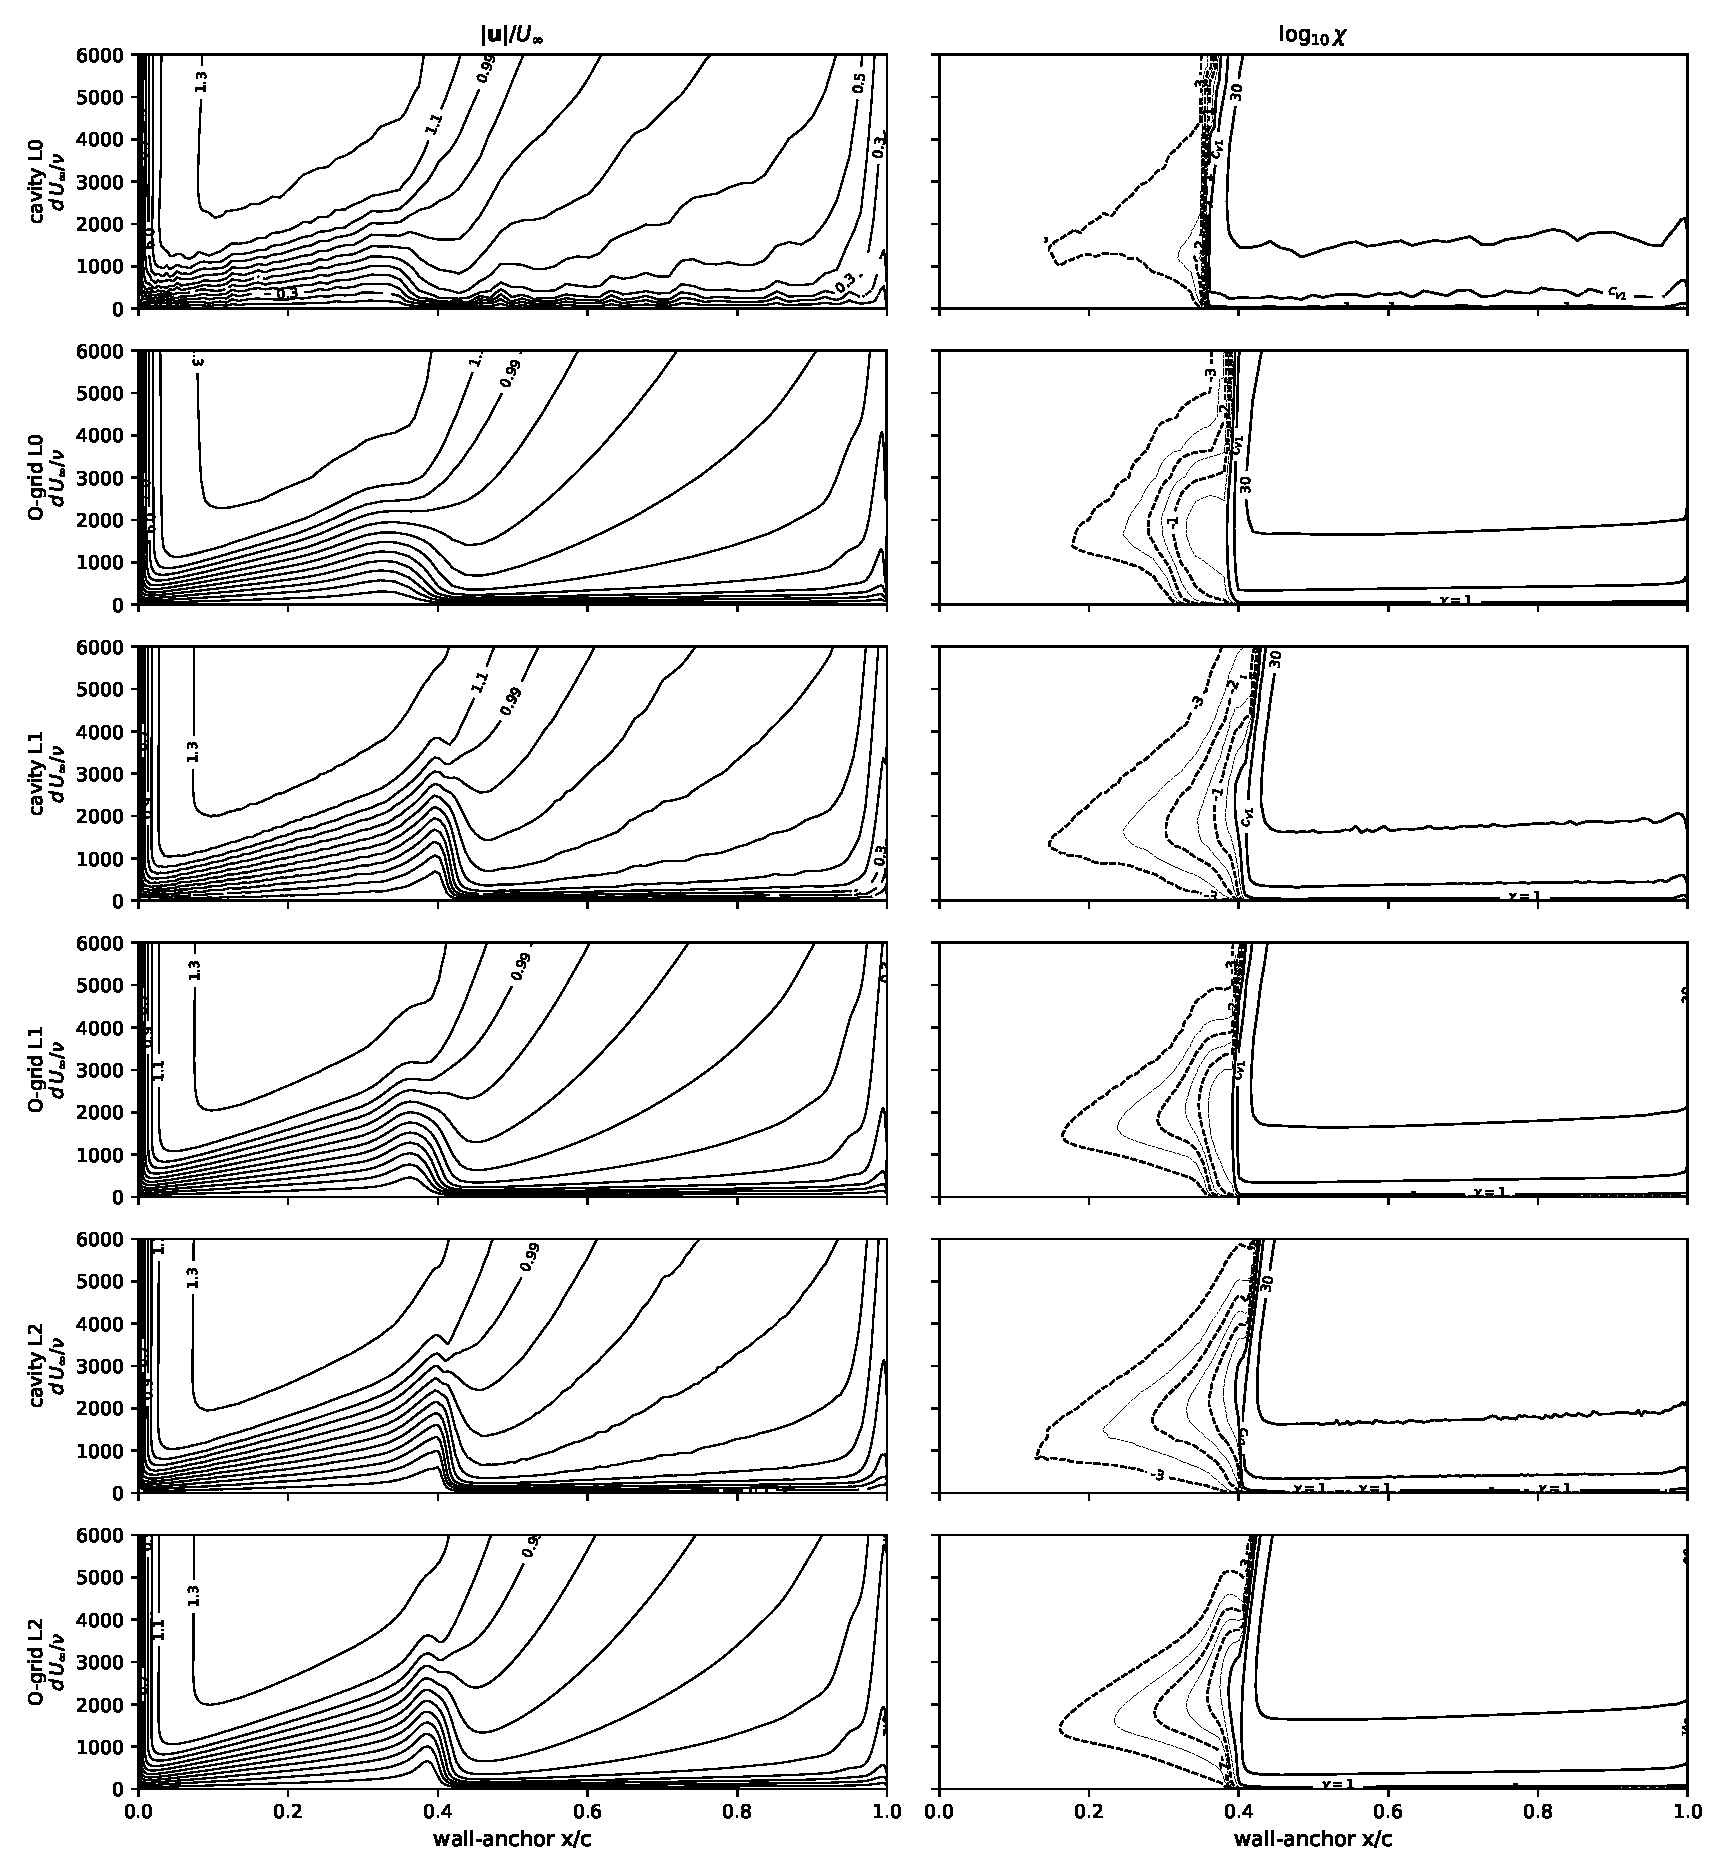
\includegraphics[width=0.99\textwidth]{chi_sheet_nlf0416_a0_upper.pdf}
  \caption{NLF(1)-0416, $Re=4\times10^6$, $\alpha=0^\circ$, upper surface: velocity magnitude (left) and $\log_{10}\chi$ (right) on all six grids.}
  \label{fig:sheet_nlf0416_a0_upper}
\end{figure}

\begin{figure}[p]
  \centering
  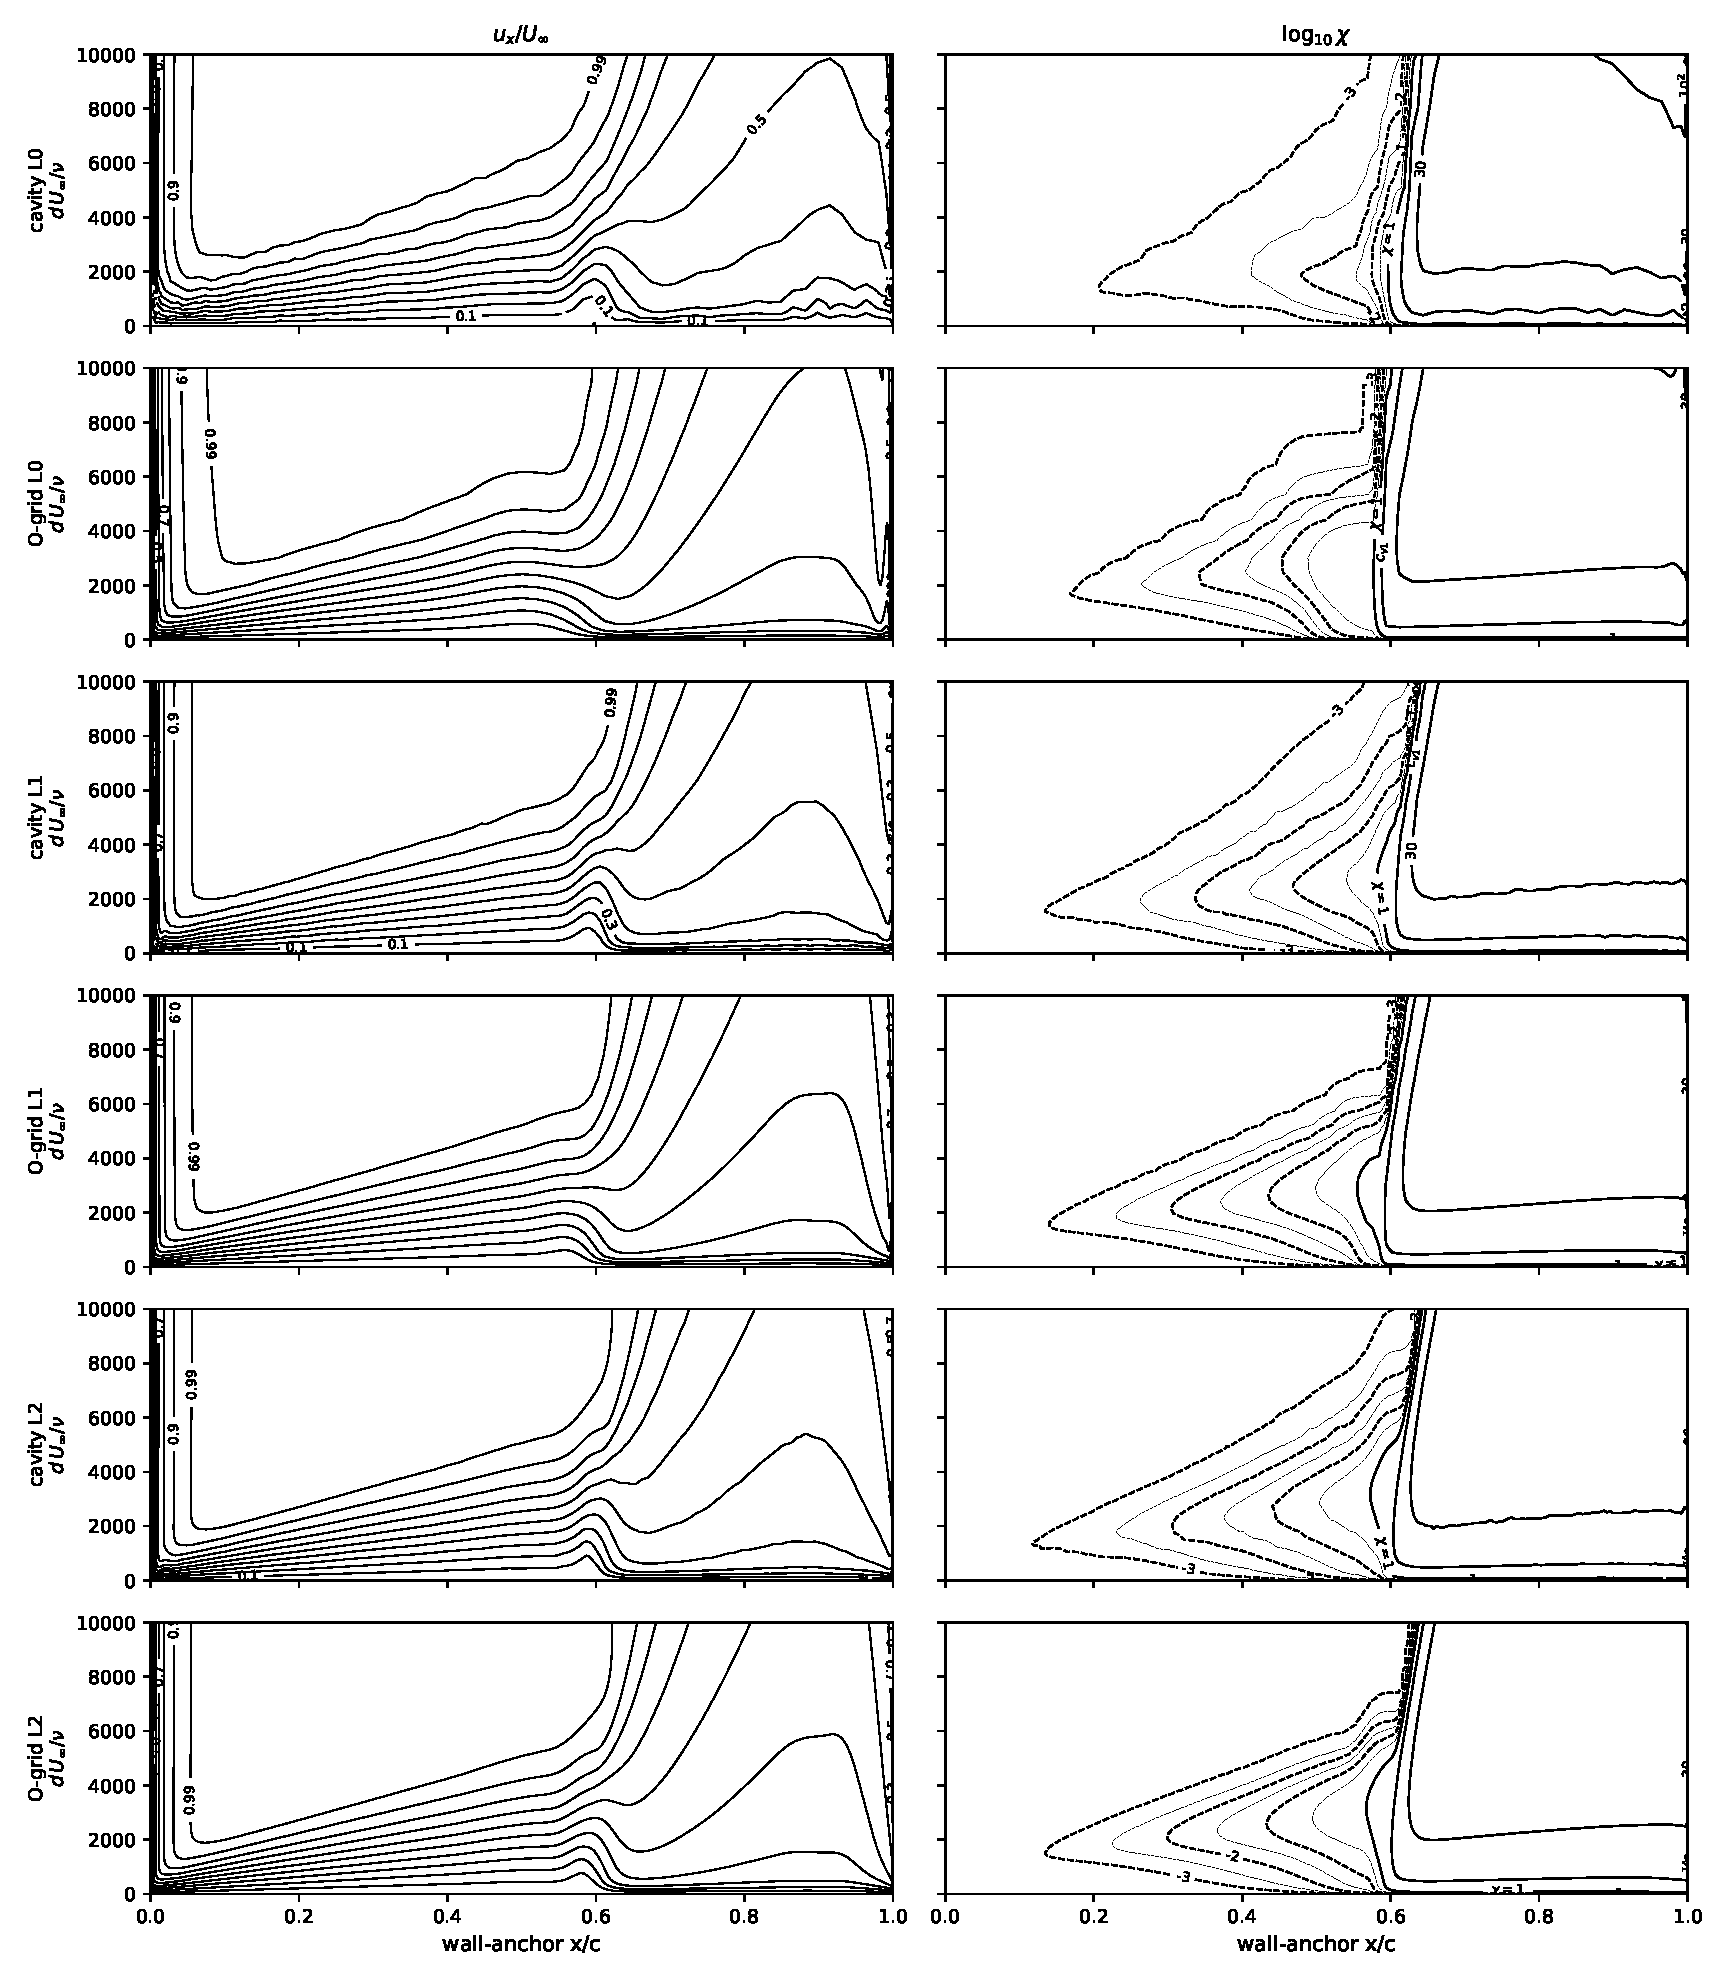
\includegraphics[width=0.99\textwidth]{chi_sheet_nlf0416_a0_lower.pdf}
  \caption{NLF(1)-0416, $Re=4\times10^6$, $\alpha=0^\circ$, lower surface: velocity magnitude (left) and $\log_{10}\chi$ (right) on all six grids.}
  \label{fig:sheet_nlf0416_a0_lower}
\end{figure}

\begin{figure}[p]
  \centering
  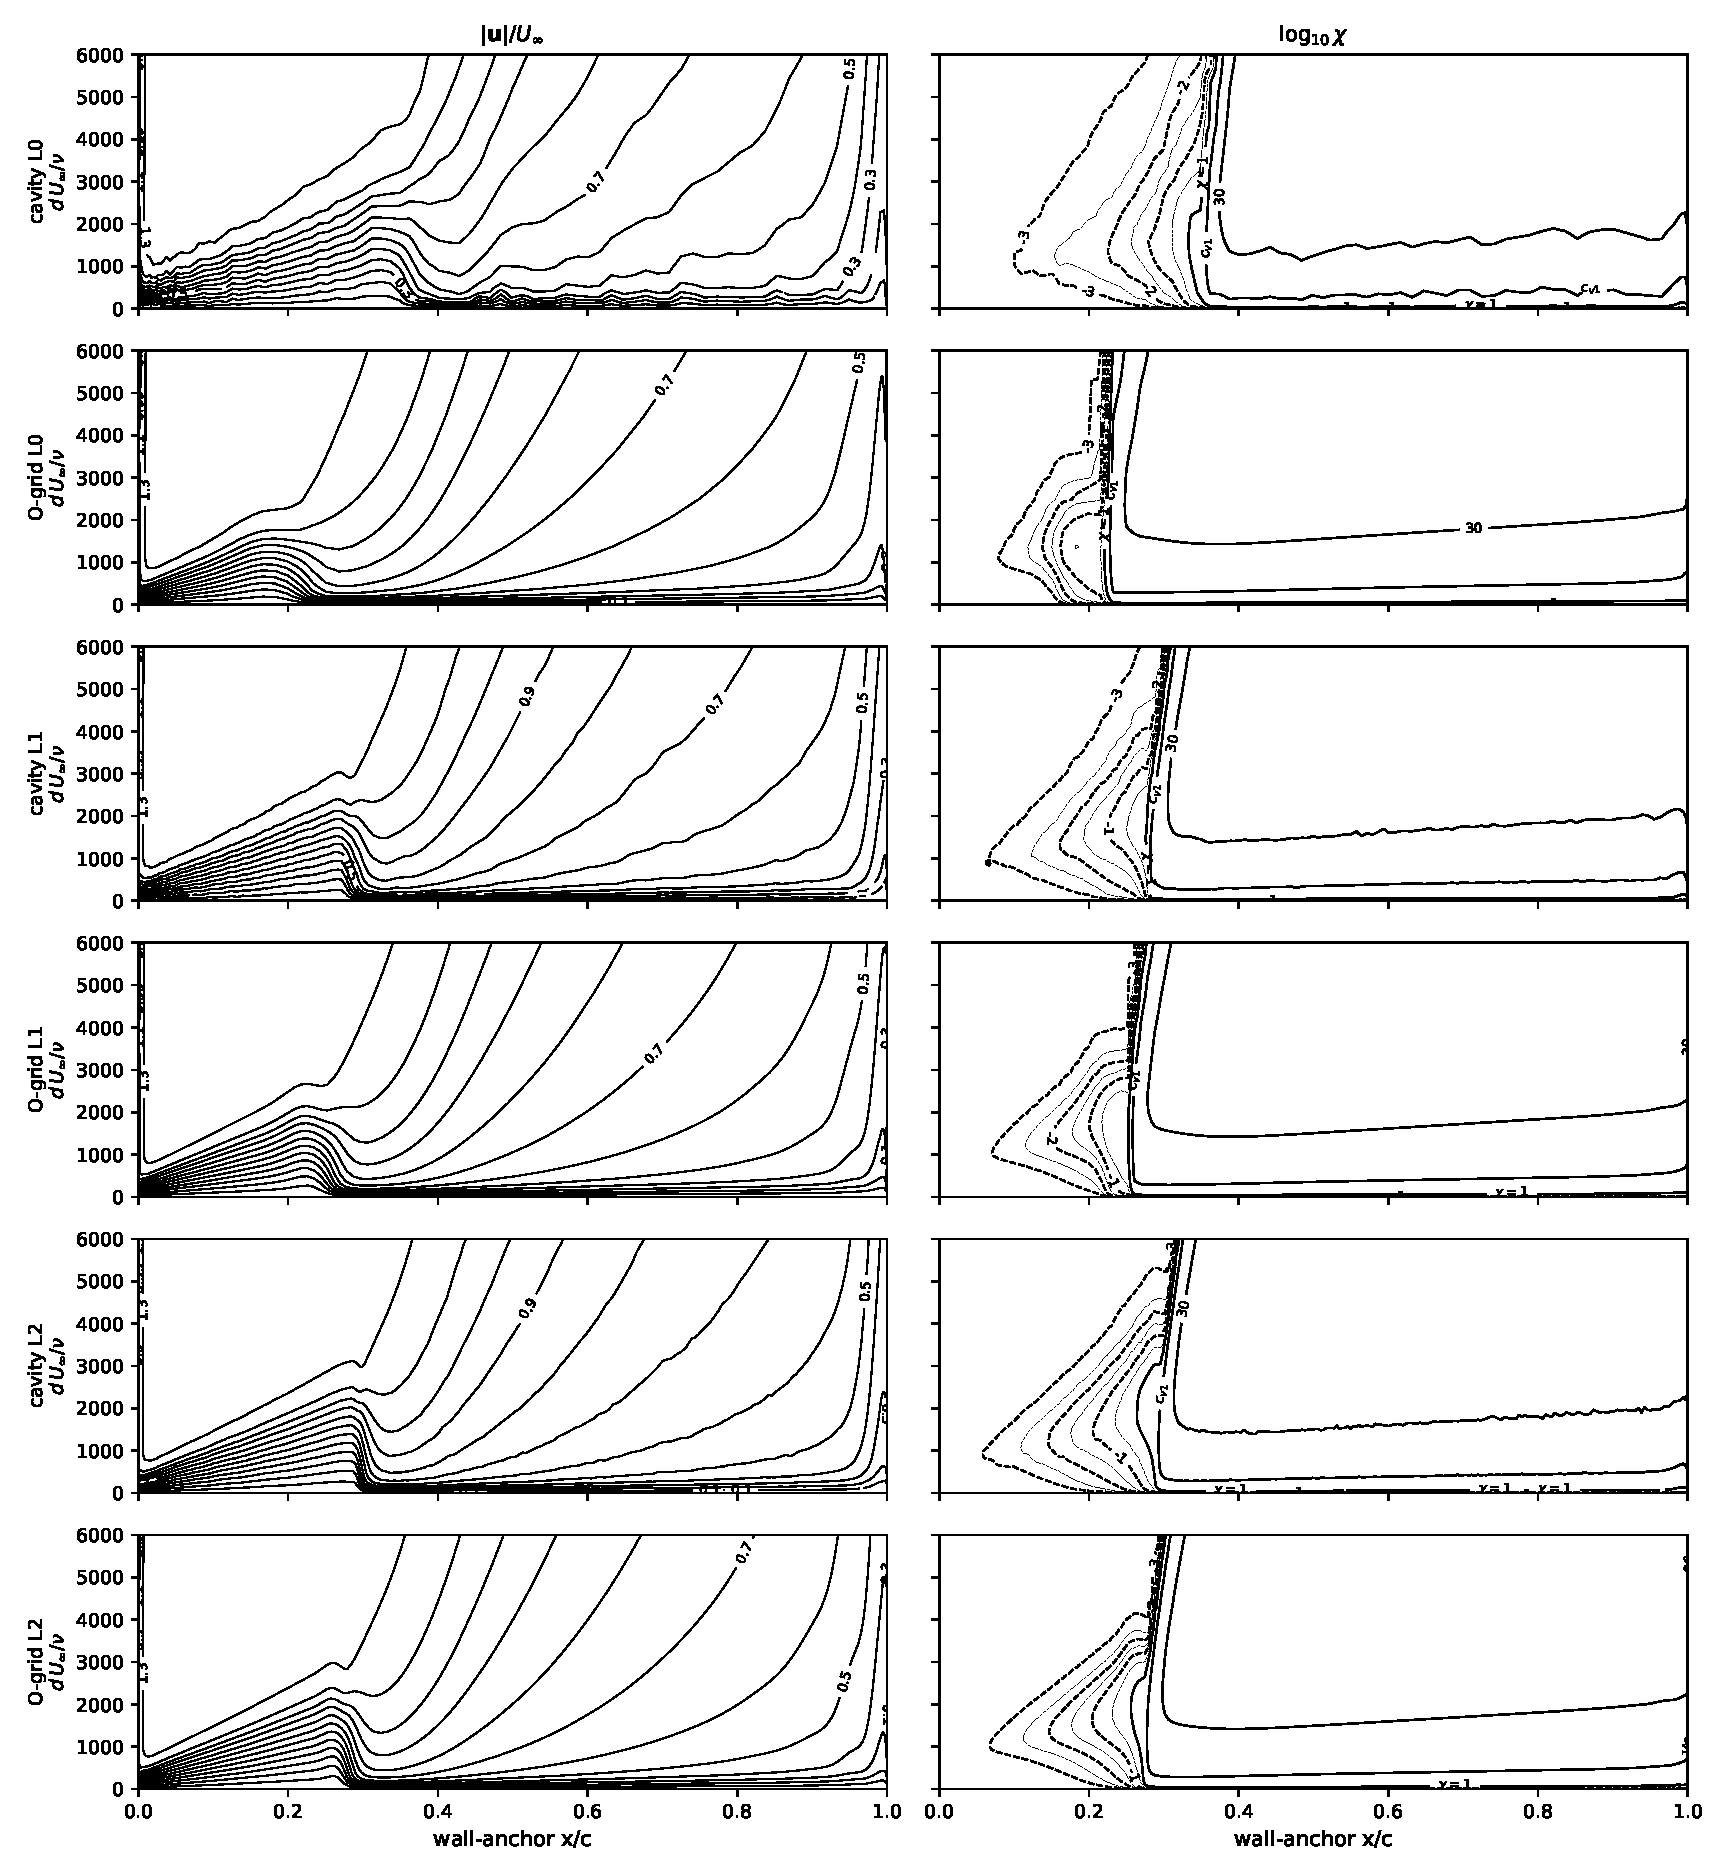
\includegraphics[width=0.99\textwidth]{chi_sheet_nlf0416_a4_upper.pdf}
  \caption{NLF(1)-0416, $Re=4\times10^6$, $\alpha=4^\circ$, upper surface: velocity magnitude (left) and $\log_{10}\chi$ (right) on all six grids.}
  \label{fig:sheet_nlf0416_a4_upper}
\end{figure}

\begin{figure}[p]
  \centering
  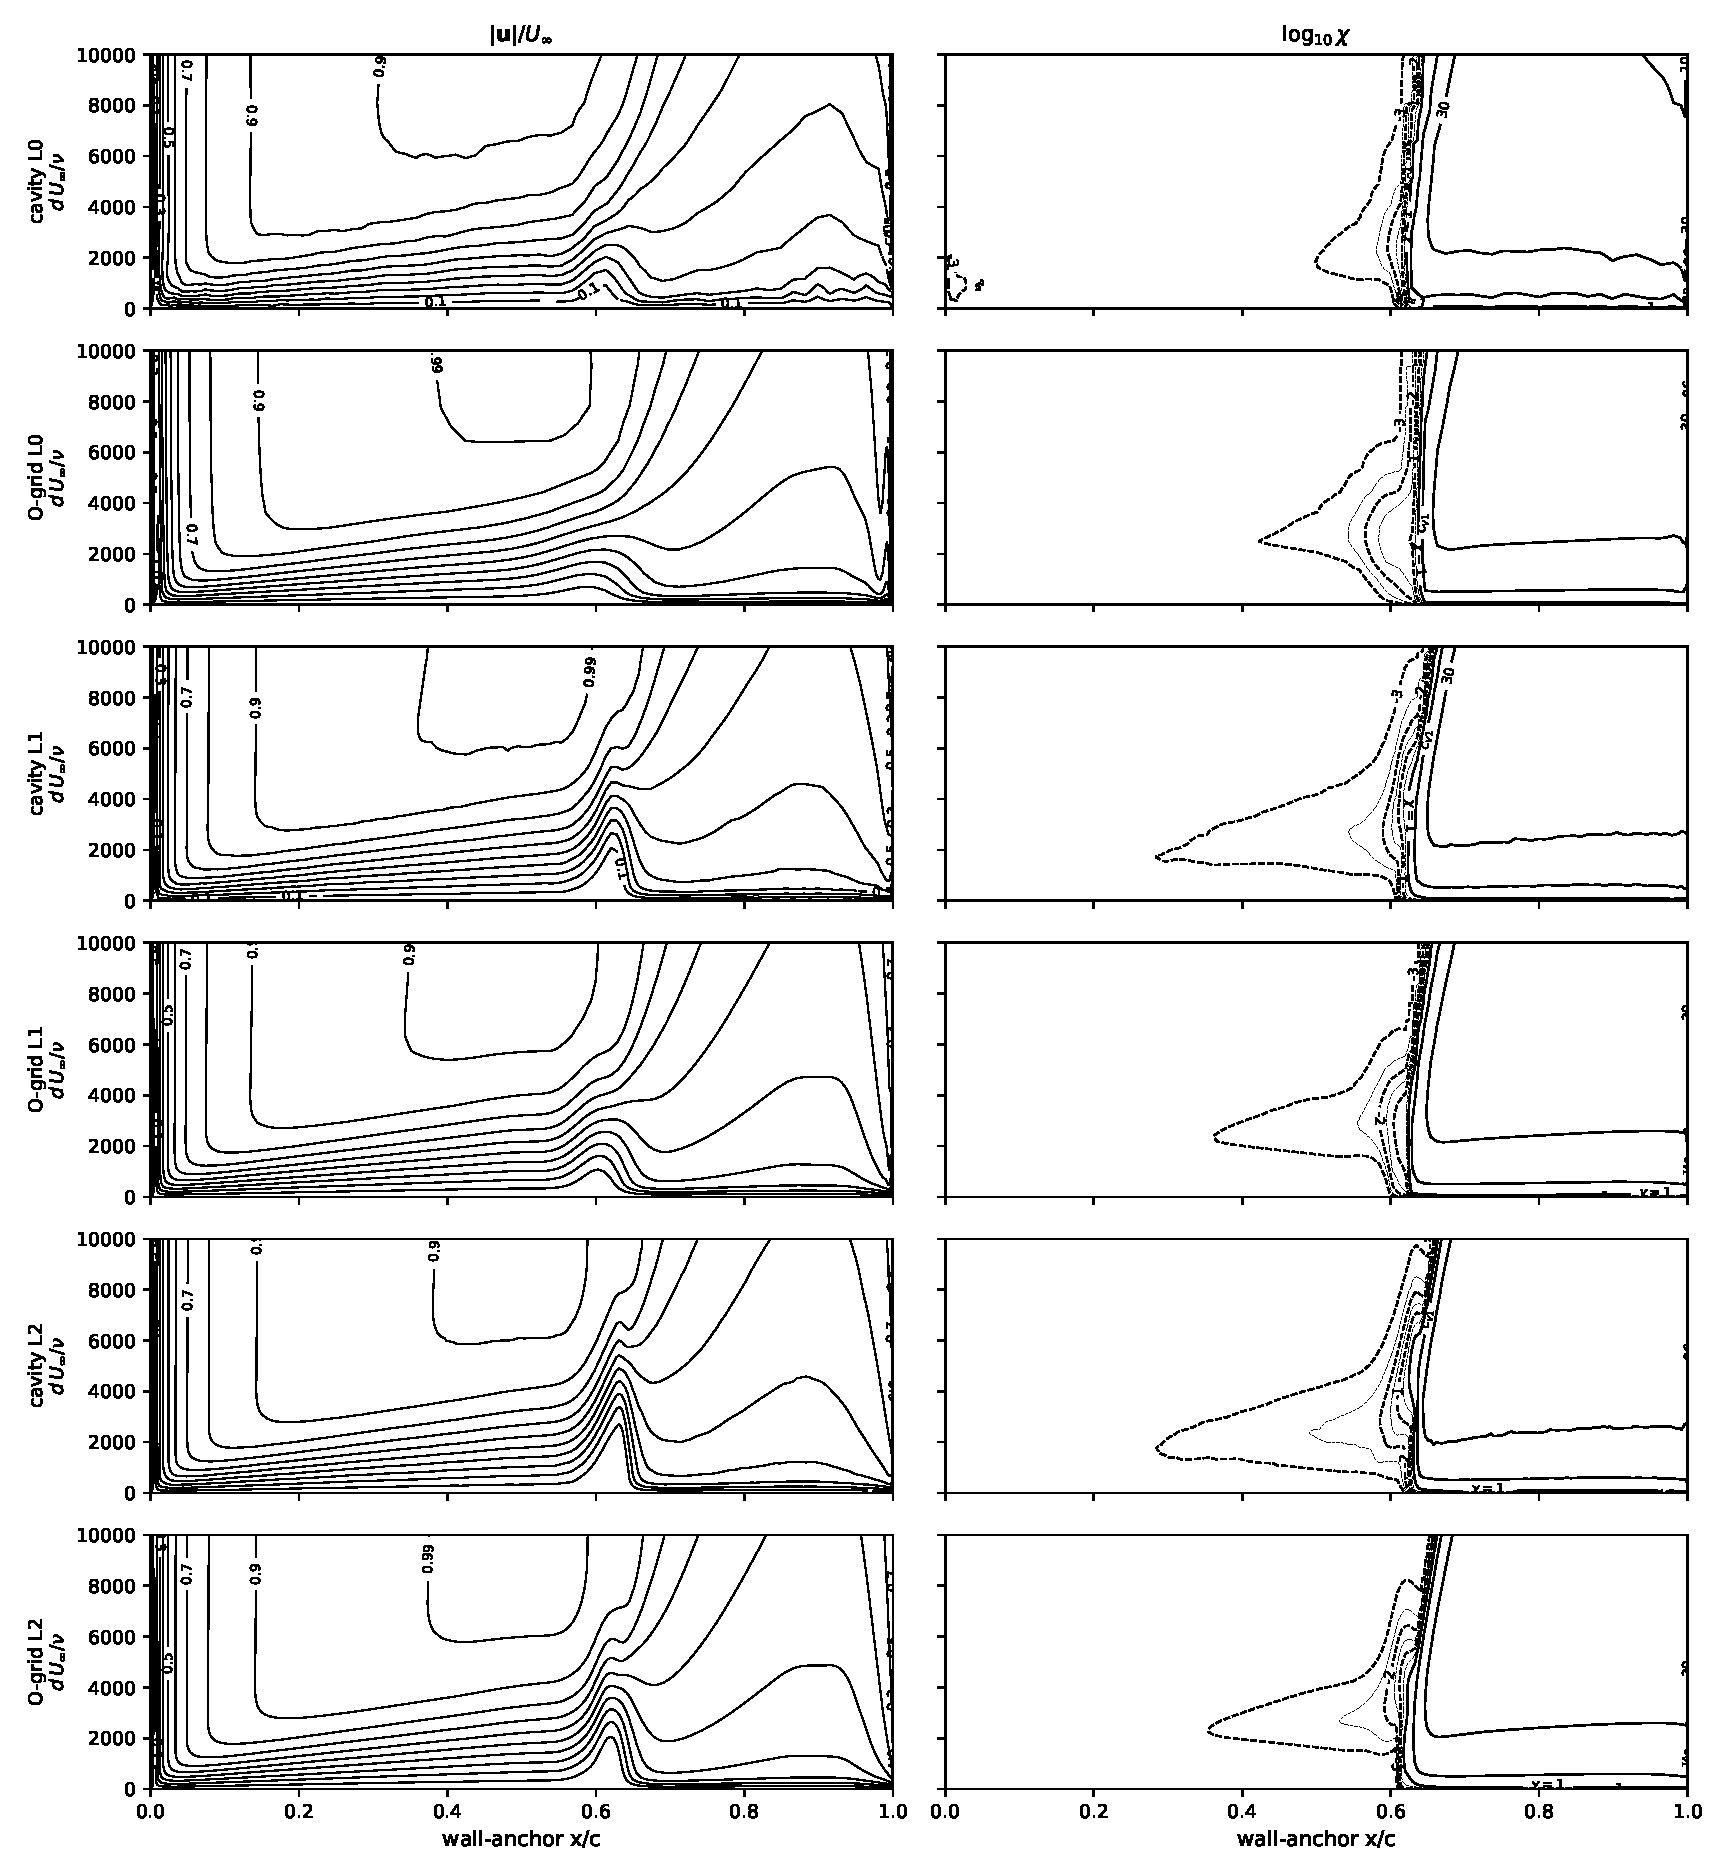
\includegraphics[width=0.99\textwidth]{chi_sheet_nlf0416_a4_lower.pdf}
  \caption{NLF(1)-0416, $Re=4\times10^6$, $\alpha=4^\circ$, lower surface: velocity magnitude (left) and $\log_{10}\chi$ (right) on all six grids.}
  \label{fig:sheet_nlf0416_a4_lower}
\end{figure}

\begin{figure}[p]
  \centering
  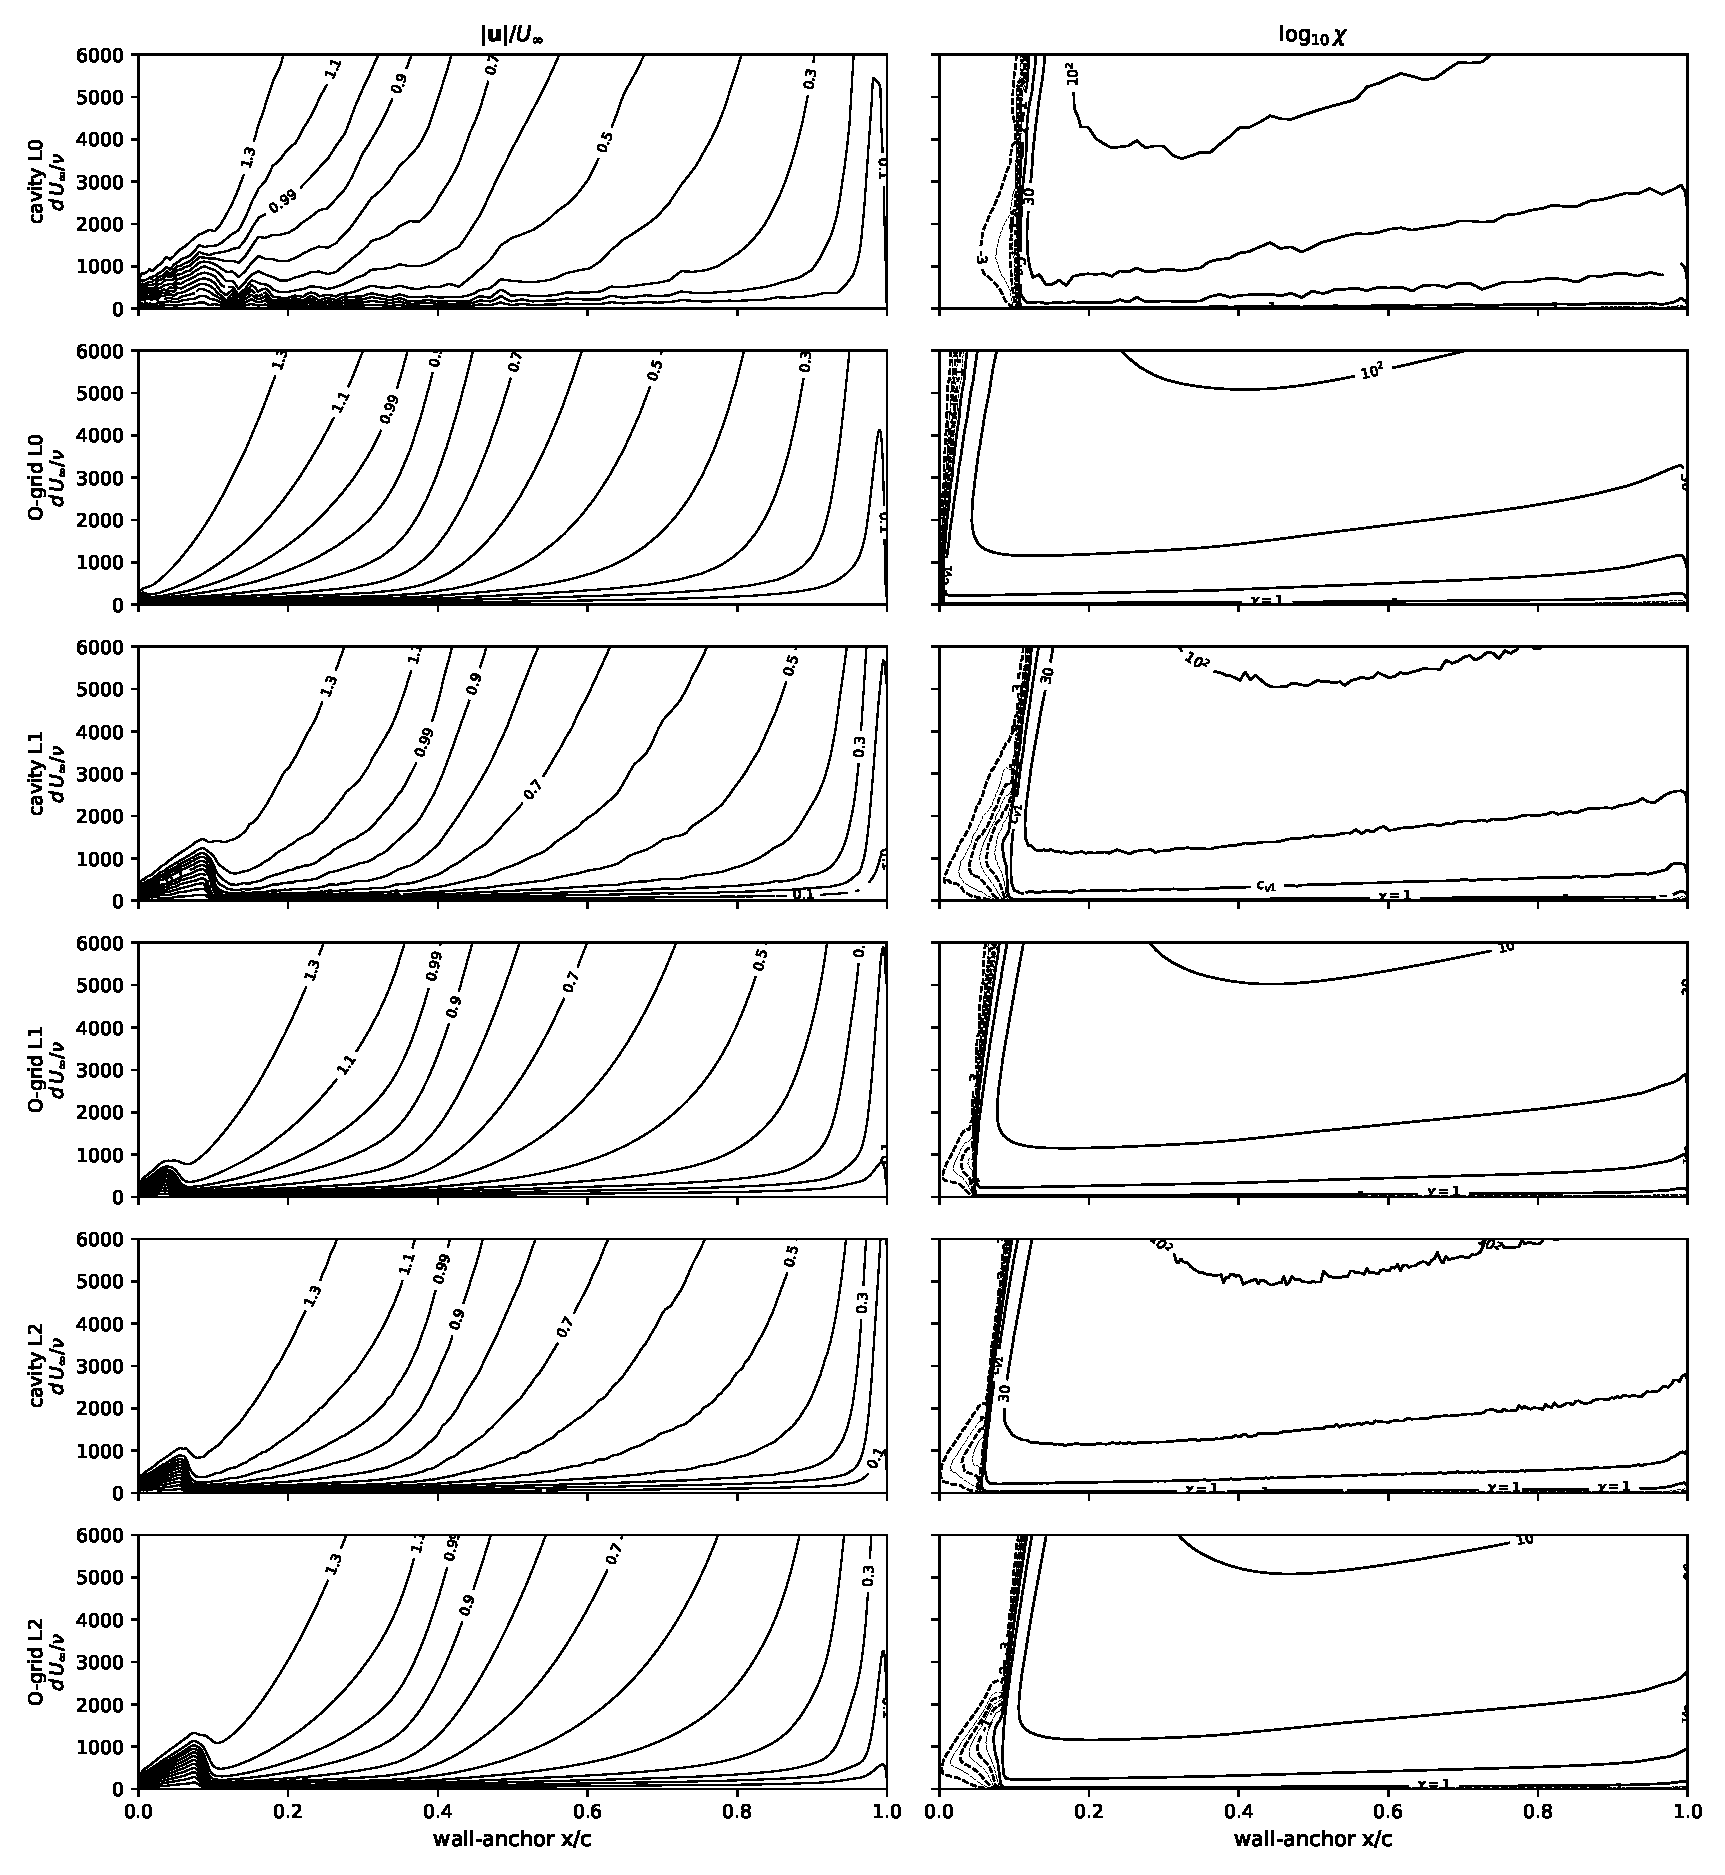
\includegraphics[width=0.99\textwidth]{chi_sheet_nlf0416_a9_upper.pdf}
  \caption{NLF(1)-0416, $Re=4\times10^6$, $\alpha=9^\circ$, upper surface: velocity magnitude (left) and $\log_{10}\chi$ (right) on all six grids.}
  \label{fig:sheet_nlf0416_a9_upper}
\end{figure}

\begin{figure}[p]
  \centering
  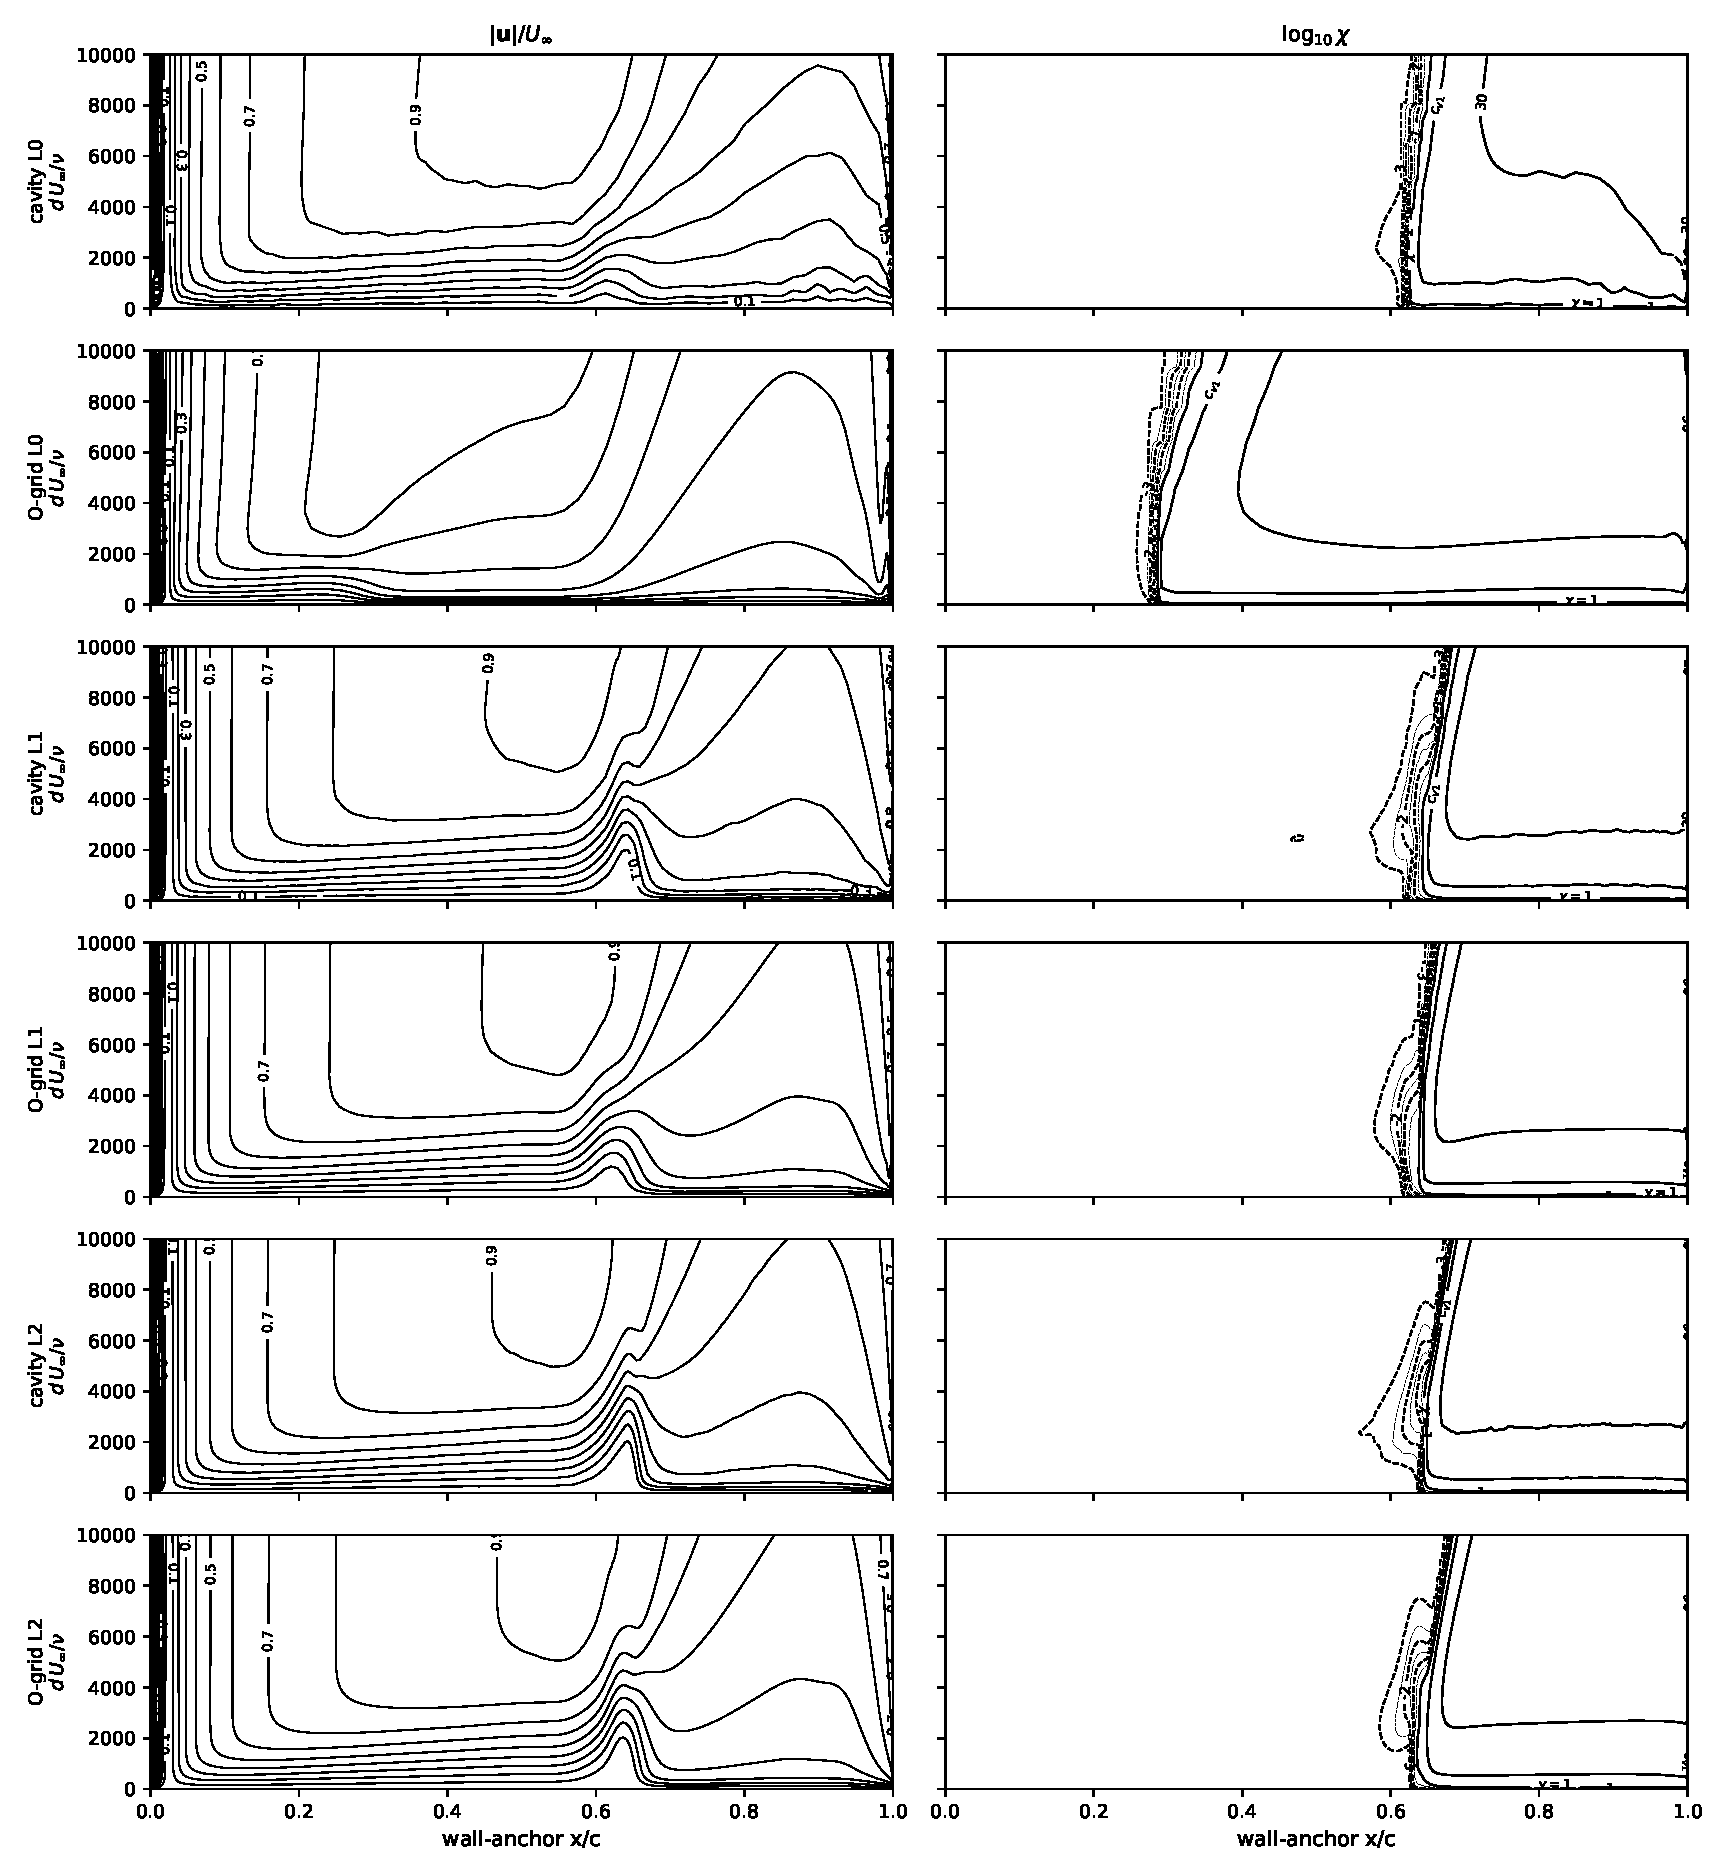
\includegraphics[width=0.99\textwidth]{chi_sheet_nlf0416_a9_lower.pdf}
  \caption{NLF(1)-0416, $Re=4\times10^6$, $\alpha=9^\circ$, lower surface: velocity magnitude (left) and $\log_{10}\chi$ (right) on all six grids.}
  \label{fig:sheet_nlf0416_a9_lower}
\end{figure}

\begin{figure}[p]
  \centering
  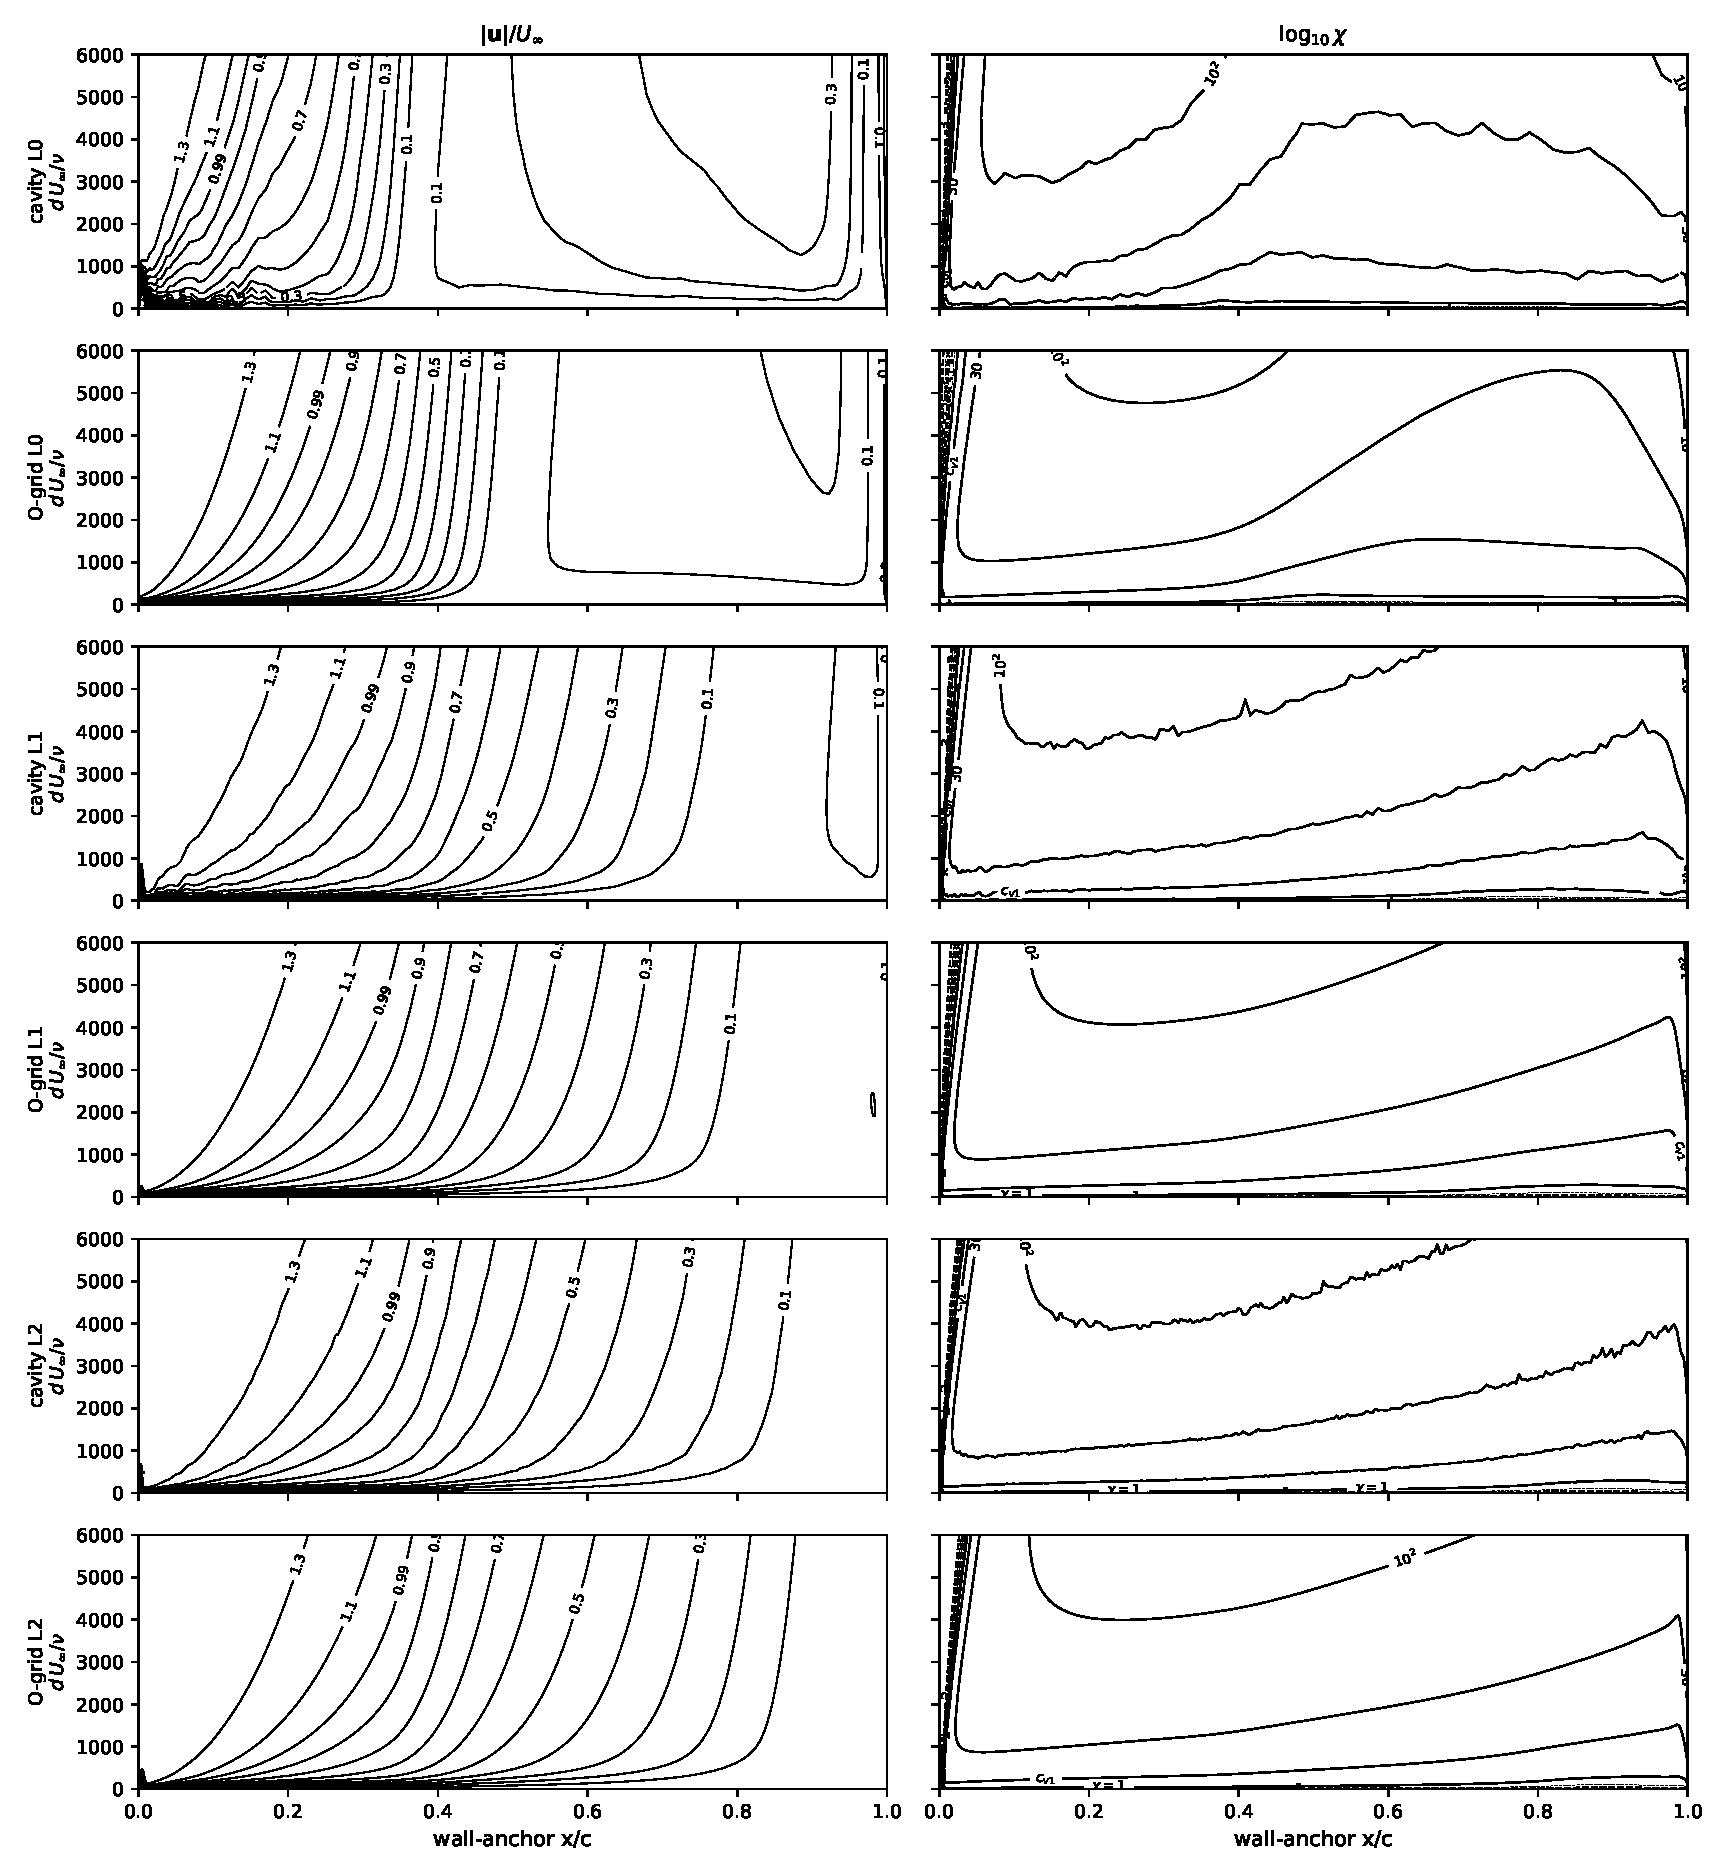
\includegraphics[width=0.99\textwidth]{chi_sheet_nlf0416_a15_upper.pdf}
  \caption{NLF(1)-0416, $Re=4\times10^6$, $\alpha=15^\circ$, upper surface: velocity magnitude (left) and $\log_{10}\chi$ (right) on all six grids.}
  \label{fig:sheet_nlf0416_a15_upper}
\end{figure}

\begin{figure}[p]
  \centering
  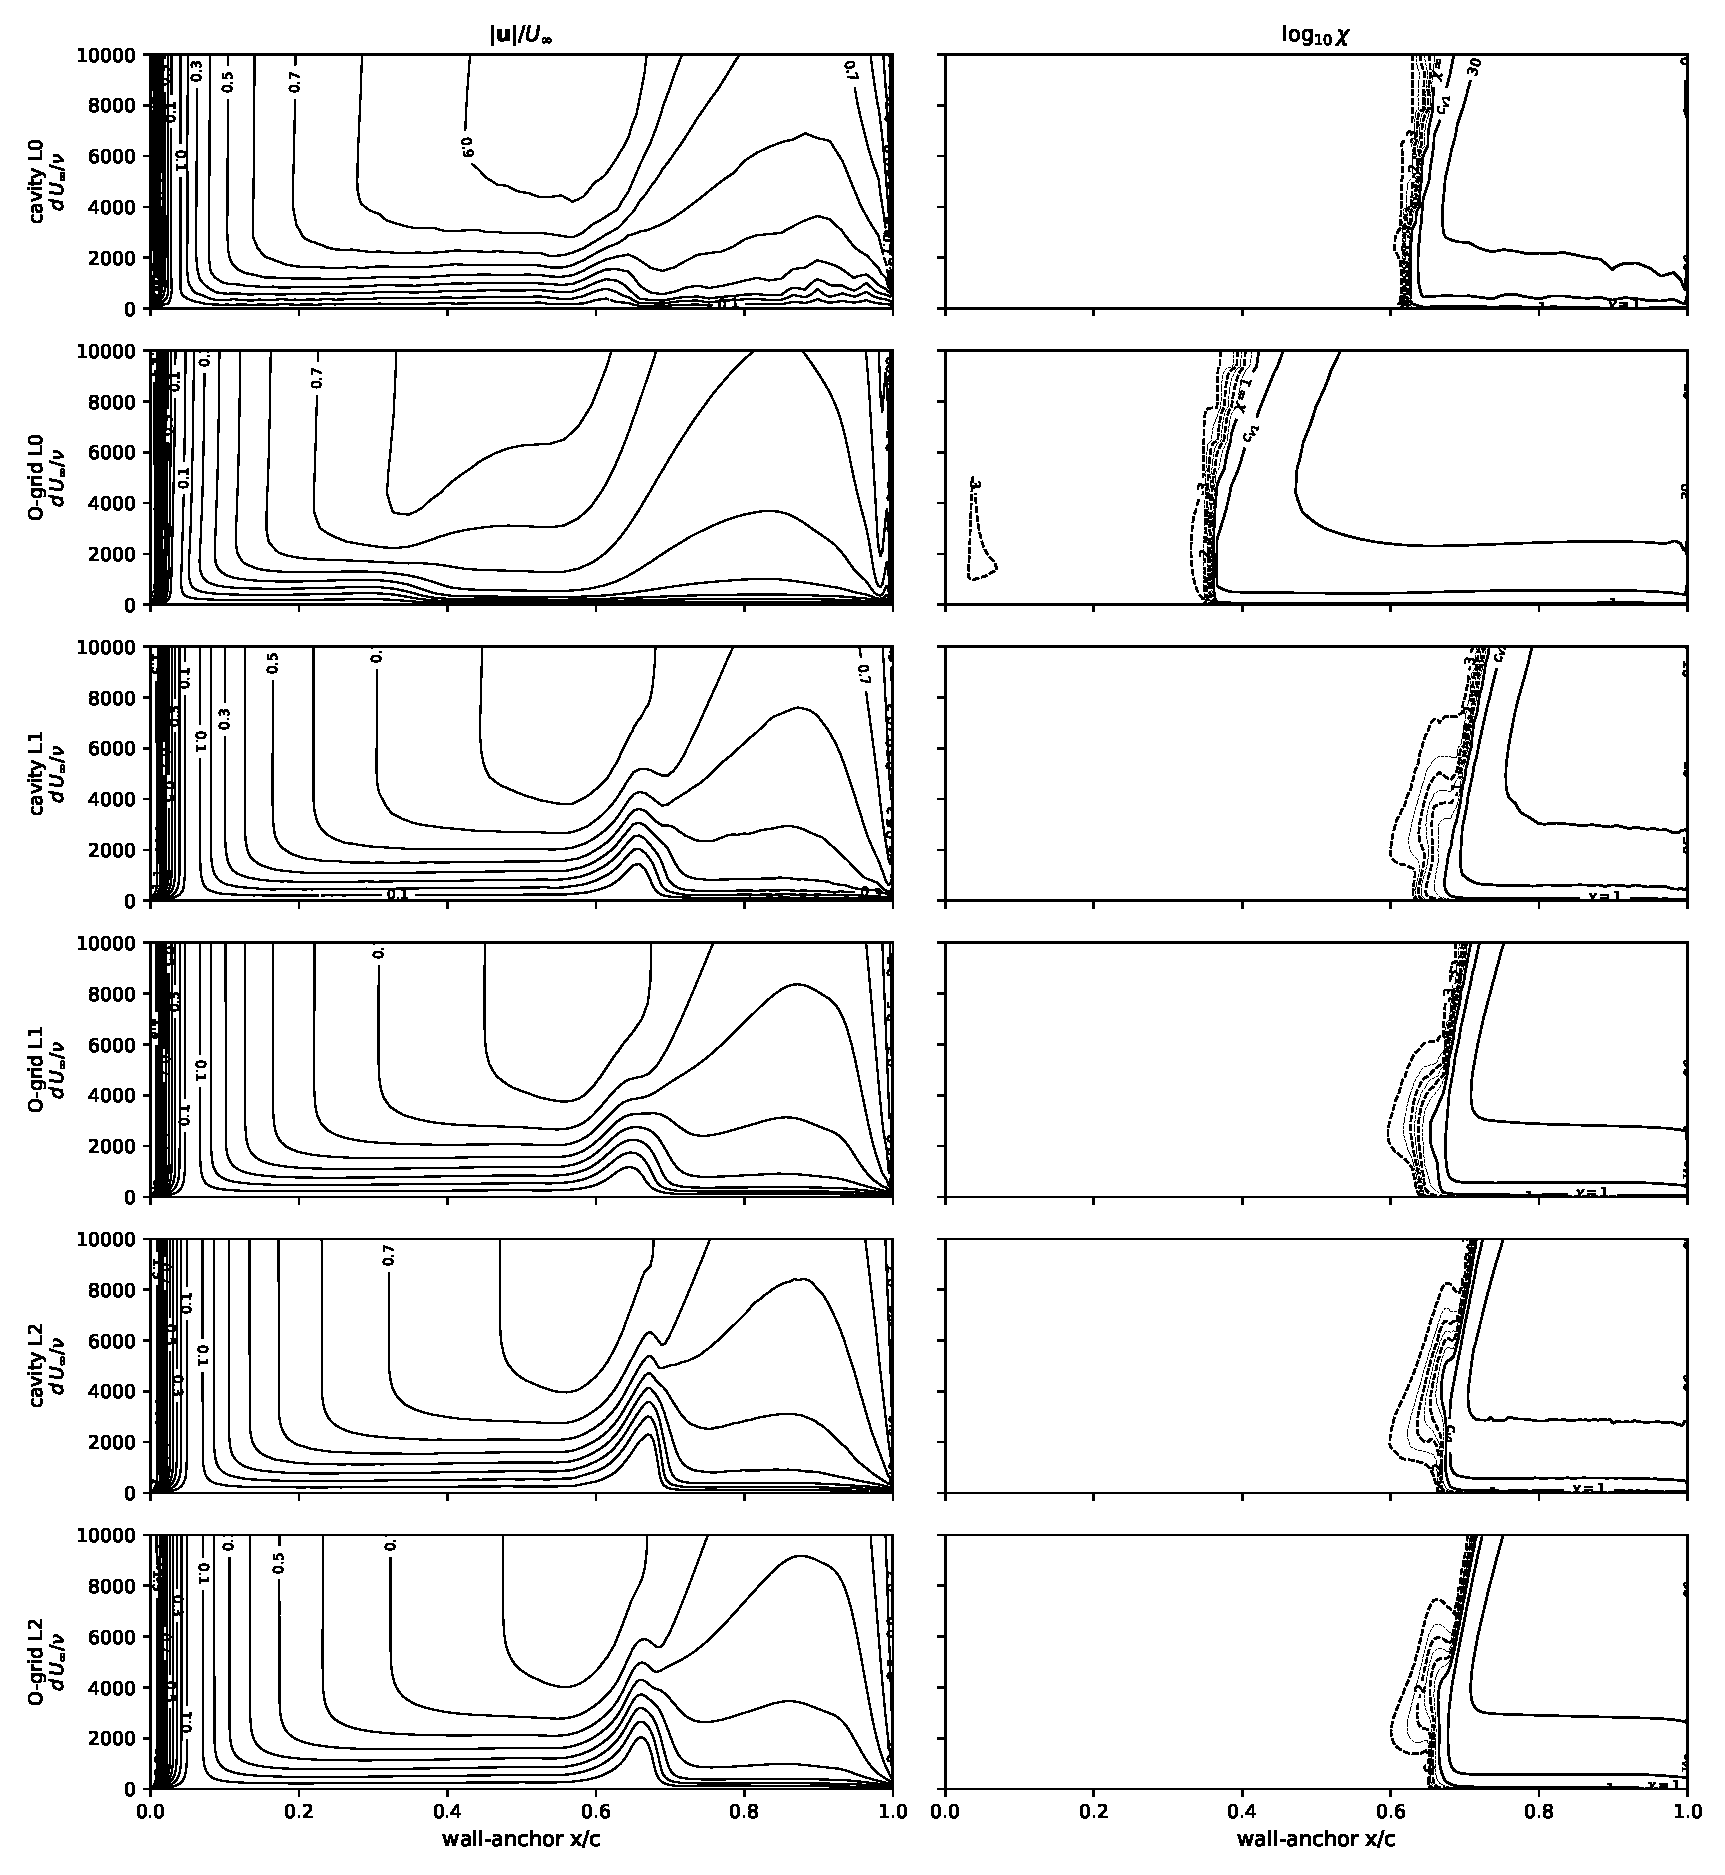
\includegraphics[width=0.99\textwidth]{chi_sheet_nlf0416_a15_lower.pdf}
  \caption{NLF(1)-0416, $Re=4\times10^6$, $\alpha=15^\circ$, lower surface: velocity magnitude (left) and $\log_{10}\chi$ (right) on all six grids.}
  \label{fig:sheet_nlf0416_a15_lower}
\end{figure}

\clearpage
\renewcommand{\thefigure}{B\arabic{figure}}
\setcounter{figure}{0}
\section*{Appendix B: the Eppler 387 benchmark---meshes and contour
sheets}

Figures~\ref{fig:eppmesh_str} and~\ref{fig:eppmesh_cav} show the mesh
close-ups for the Eppler benchmark of Sec.~\ref{sec:eppval}; the sheets
that follow cover the $\alpha$ sweep at $Re=2\times10^5$ in ascending
incidence, including the $-2^\circ$ and $8.5^\circ$ extension pair
(finest grids only), upper
surface only---the lower surface stays attached and featureless
throughout the sweep (wall-normal frame $0.0335c$, the
$5\times$-raised handover frame of the Appendix~A conventions).

The $\alpha\!=\!5^\circ$ sheet
(Fig.~\ref{fig:sheet_eppler387_a5_upper}) also resolves the anatomy
of the double peak that the $\max_y \hat\Omega \hat I$ trace of
Fig.~\ref{fig:eppcflow} (row~2, a wall-normal probe of fixed depth
$0.01\,c$, neighbor-smoothed as stated in Sec.~\ref{sec:nlfval})
shows inside the bubble. The first peak is the \emph{lifted laminar
shear layer} over the recirculation core: at its maximum ($0.92$ at
$x\!\approx\!0.50$) the rate-carrying layer has climbed to the top
of the probe window ($0.01\,c$, roughly $y^+\!\approx\!40$ in the
viscous units of the reattached wall)---visible in the sheet as the
elevated high-shear band arcing over the bubble. The notch that
follows (minimum ${\approx}0.28$ at $x\!=\!0.54$; deeper in the
raw pointwise trace) is the layer \emph{leaving that fixed window},
not a collapse of the physical field: probed at full depth, the
lifted layer stays saturated ($\hat\Omega \hat I\!\approx\!1$)
just above the window until $x\!\approx\!0.6$, and the full-depth
envelope never drops below $0.9$ between the peaks. With the strong
outer branch out of frame, the trace shows the still-weak near-wall
region, then re-rises as the layer descends through reattachment: the
second peak ($0.82$ at $x\!=\!0.615$) is the new near-wall
\emph{reattachment layer} (at a few thousandths of a chord,
$y^+\!\sim\!6$, the sublayer of the forming turbulent wall layer),
with concentrated shear at the low advection speed of the
reattachment region saturating $\hat\Omega \hat I$ once more before
the attached-boundary-layer level (${\approx}0.08$) takes over
downstream. The handover crossings ($\chi\!=\!1$ at $0.48$,
$c_{v1}$ at $0.54$, $30$ at $0.59$) bracket the notch because both
track the bubble's growth toward reattachment; the alignment is
correlational, not causal.

\begin{figure}[p]
  \centering
  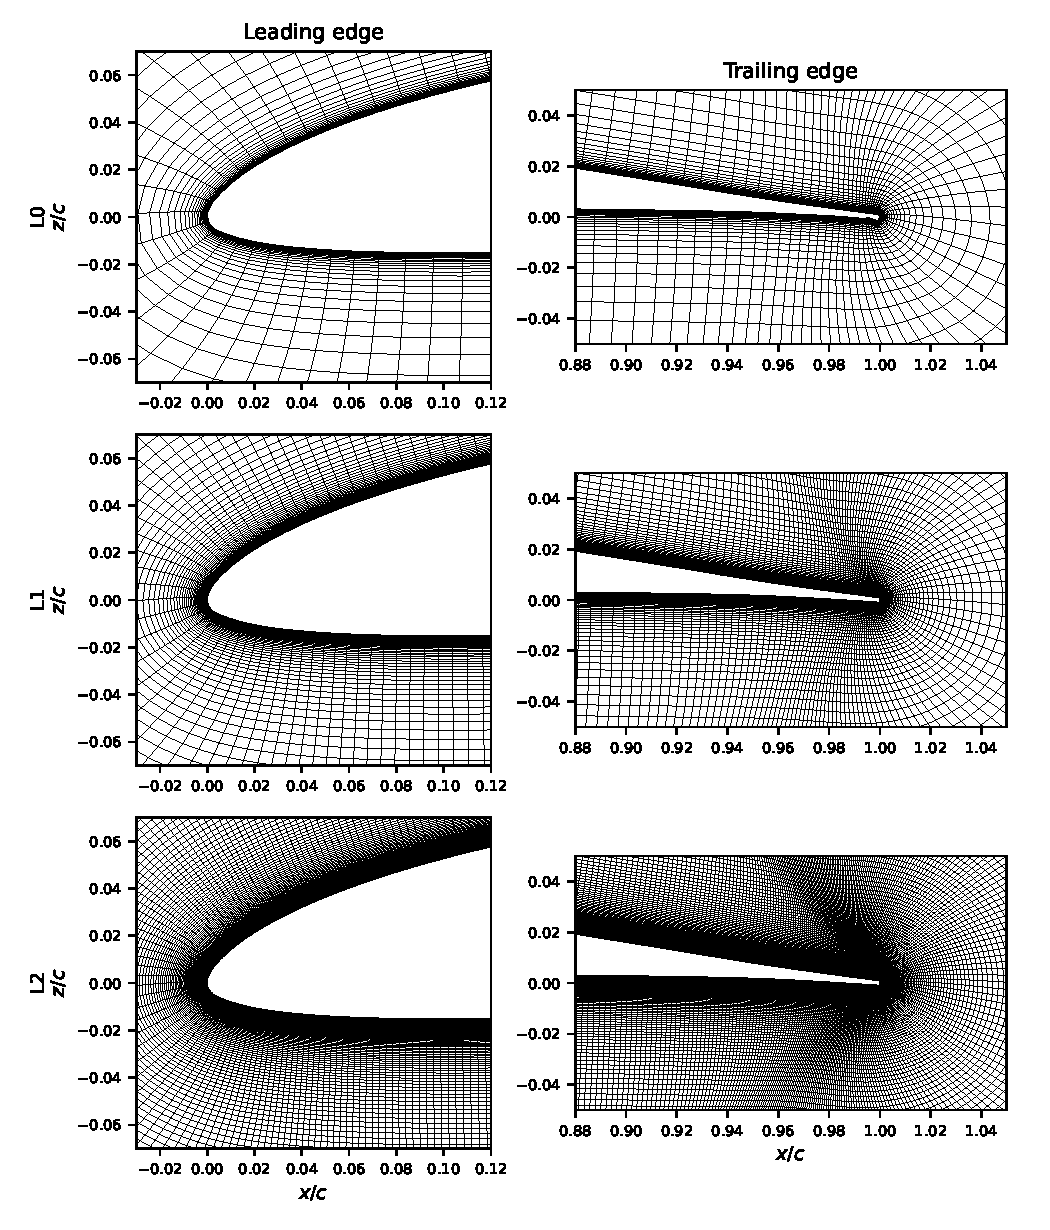
\includegraphics[width=\textwidth,height=0.92\textheight,keepaspectratio]{mesh_eppler_str.pdf}
  \caption{Eppler 387 structured O-grid mesh at the leading edge (left column)
  and trailing edge (right column) for the three refinement levels L0--L2
  (rows), generated by the same recipe as the NLF grid
  (Fig.~\ref{fig:nlfmesh_str}); every length scale halves per level. Chord
  normalized to unity ($z$ vertical).}
  \label{fig:eppmesh_str}
\end{figure}

\begin{figure}[p]
  \centering
  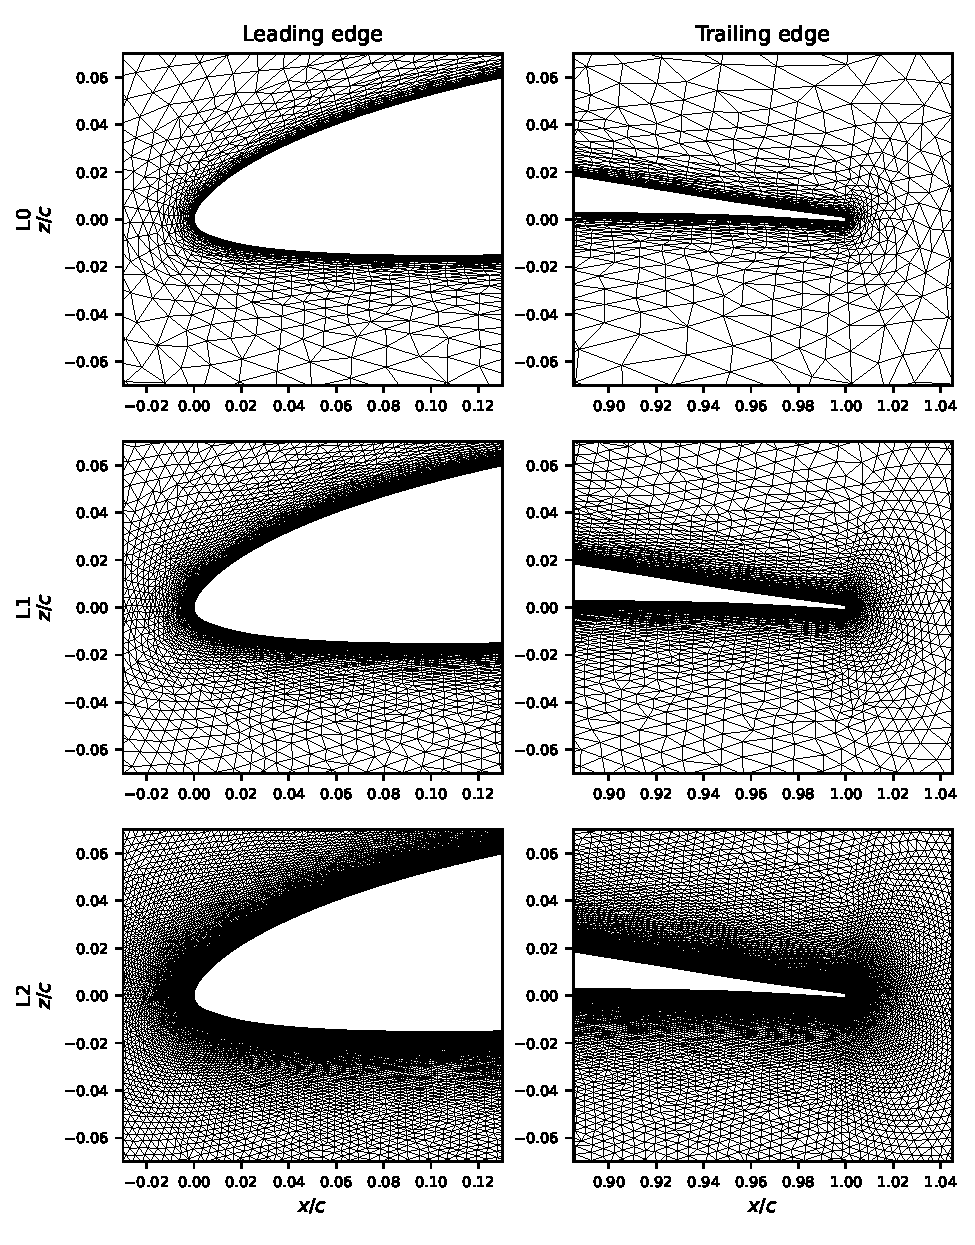
\includegraphics[width=\textwidth,height=0.92\textheight,keepaspectratio]{mesh_eppler_cav.pdf}
  \caption{Eppler 387 unstructured cavity mesh (leading and trailing edges,
  levels L0--L2), built from the same arc-length cubic-spline contour as the structured grid of
  Fig.~\ref{fig:eppmesh_str} with an anisotropic near-wall boundary-layer
  region; every length scale halves per level.}
  \label{fig:eppmesh_cav}
\end{figure}

\begin{figure}[p]
  \centering
  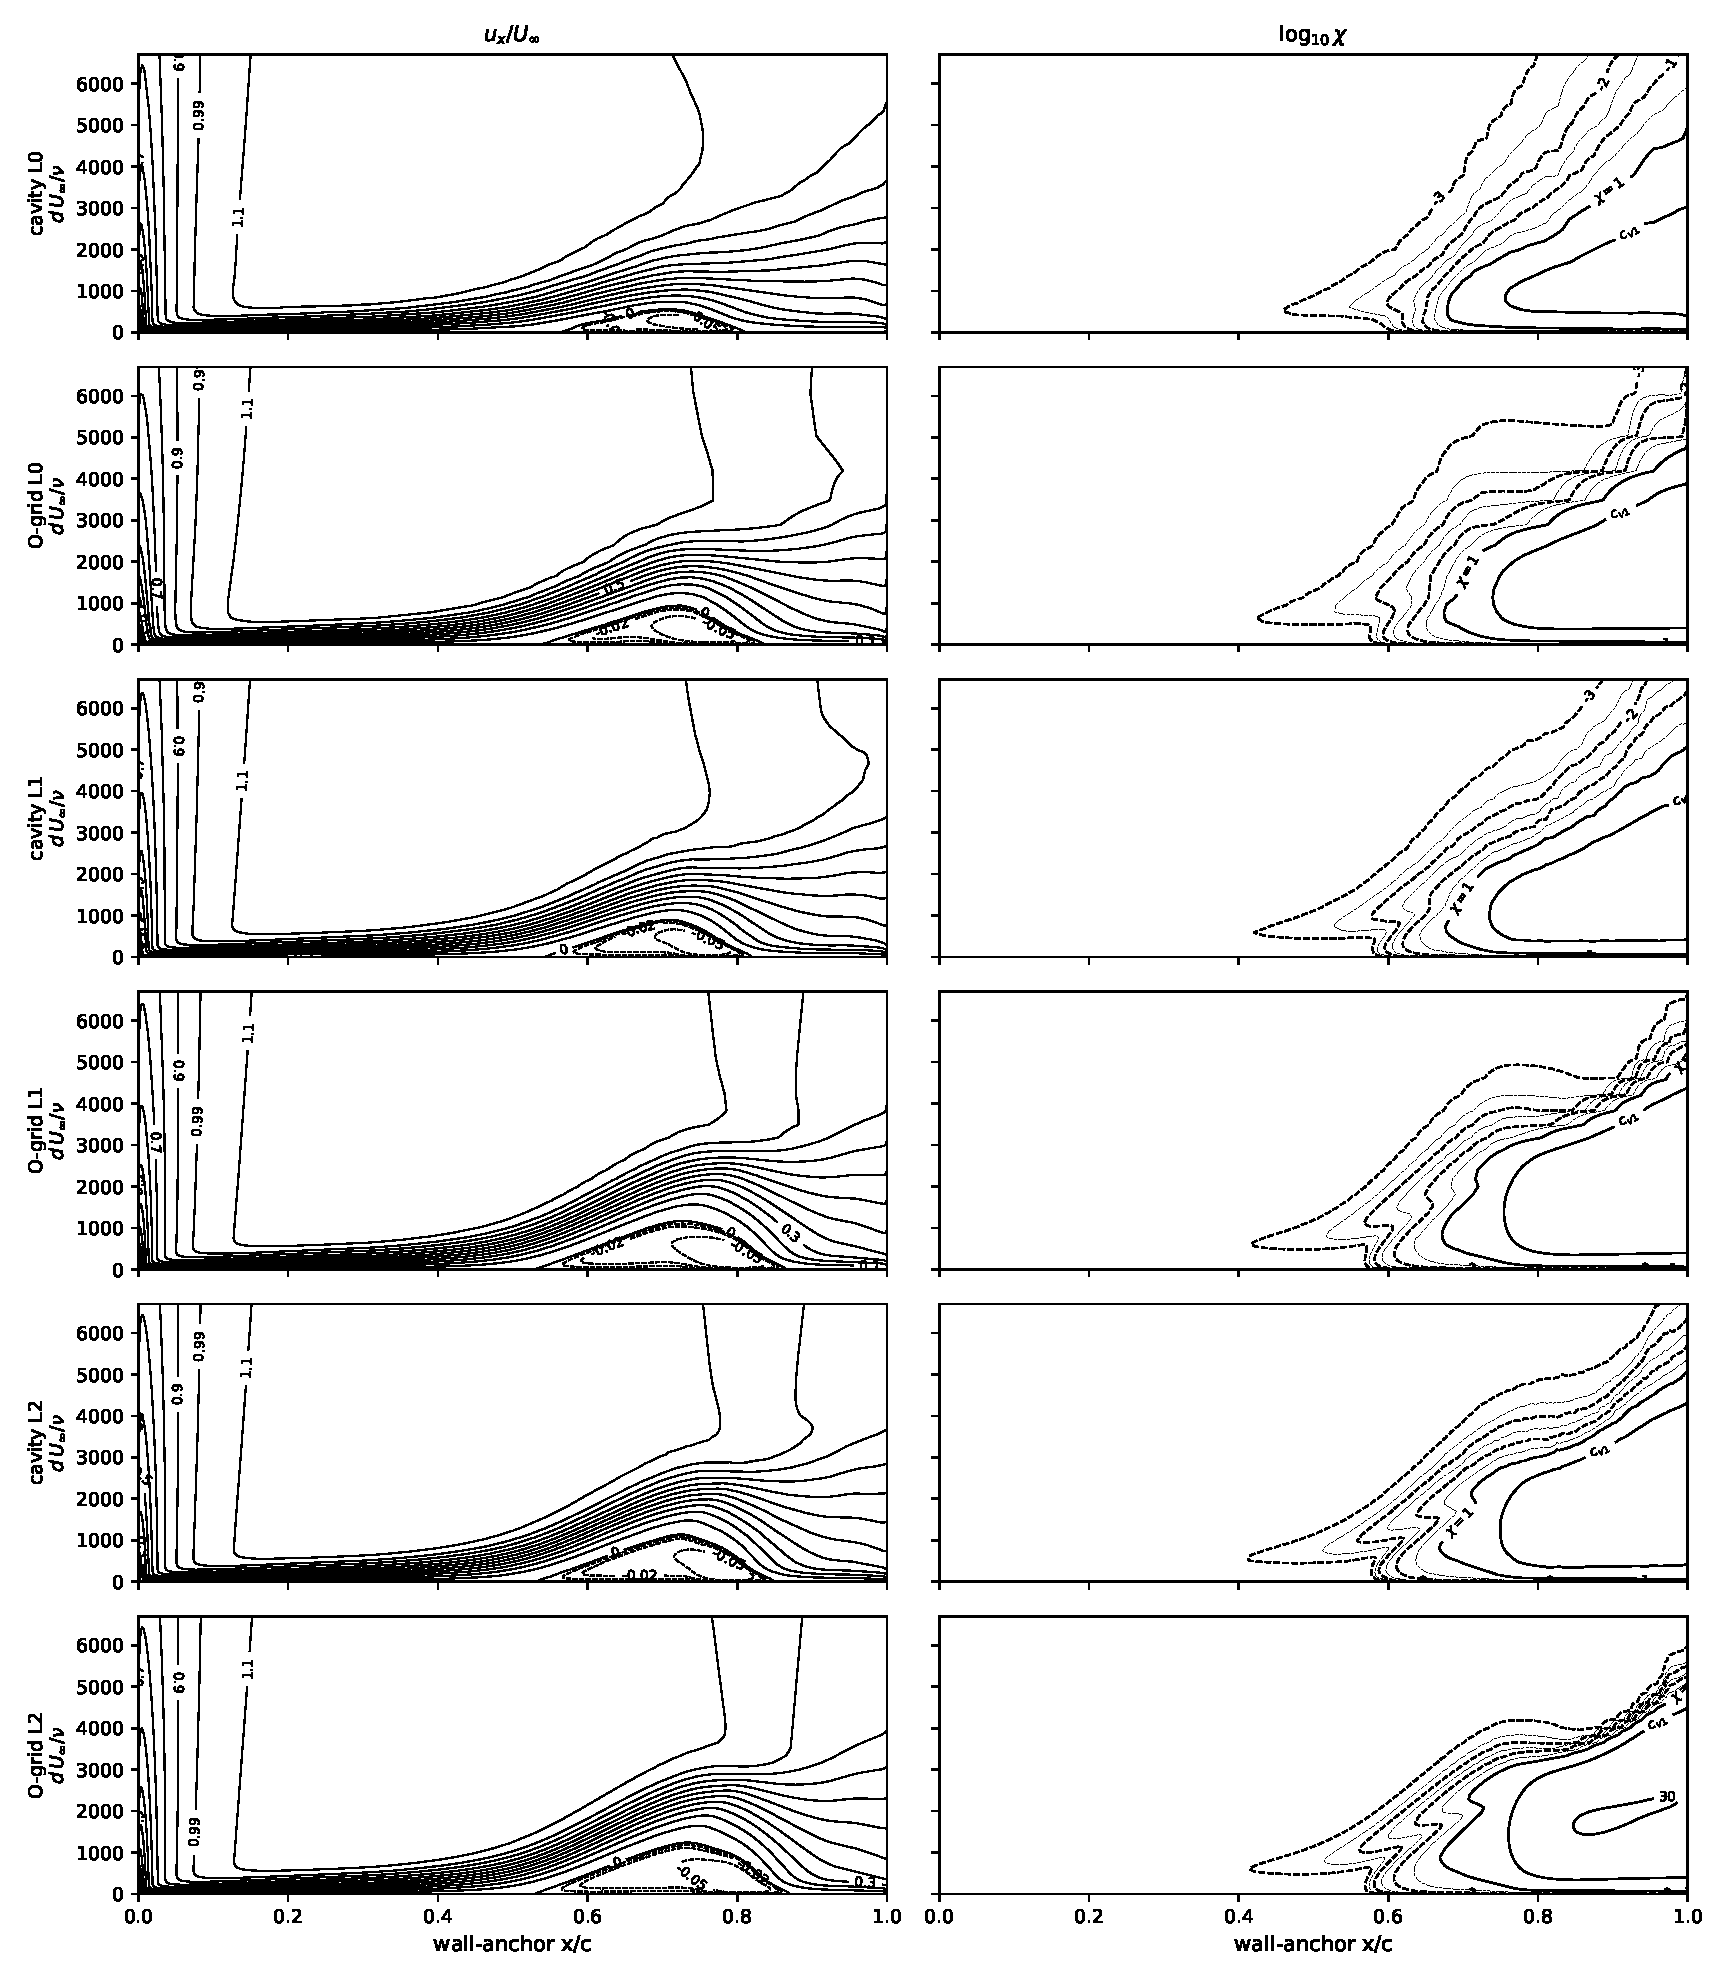
\includegraphics[width=0.99\textwidth]{chi_sheet_eppler387_am2_upper.pdf}
  \caption{Eppler~387, $Re=2\times10^5$, $\alpha=-2^\circ$, upper
  surface (finest L2 pair; the extension incidences exist on L2 only):
  velocity magnitude (left) and $\log_{10}\chi$ (right). The bubble
  sits at its aft-most station of the sweep
  ($x/c\!\approx\!0.55$--$0.80$).}
  \label{fig:sheet_eppler387_am2_upper}
\end{figure}

\begin{figure}[p]
  \centering
  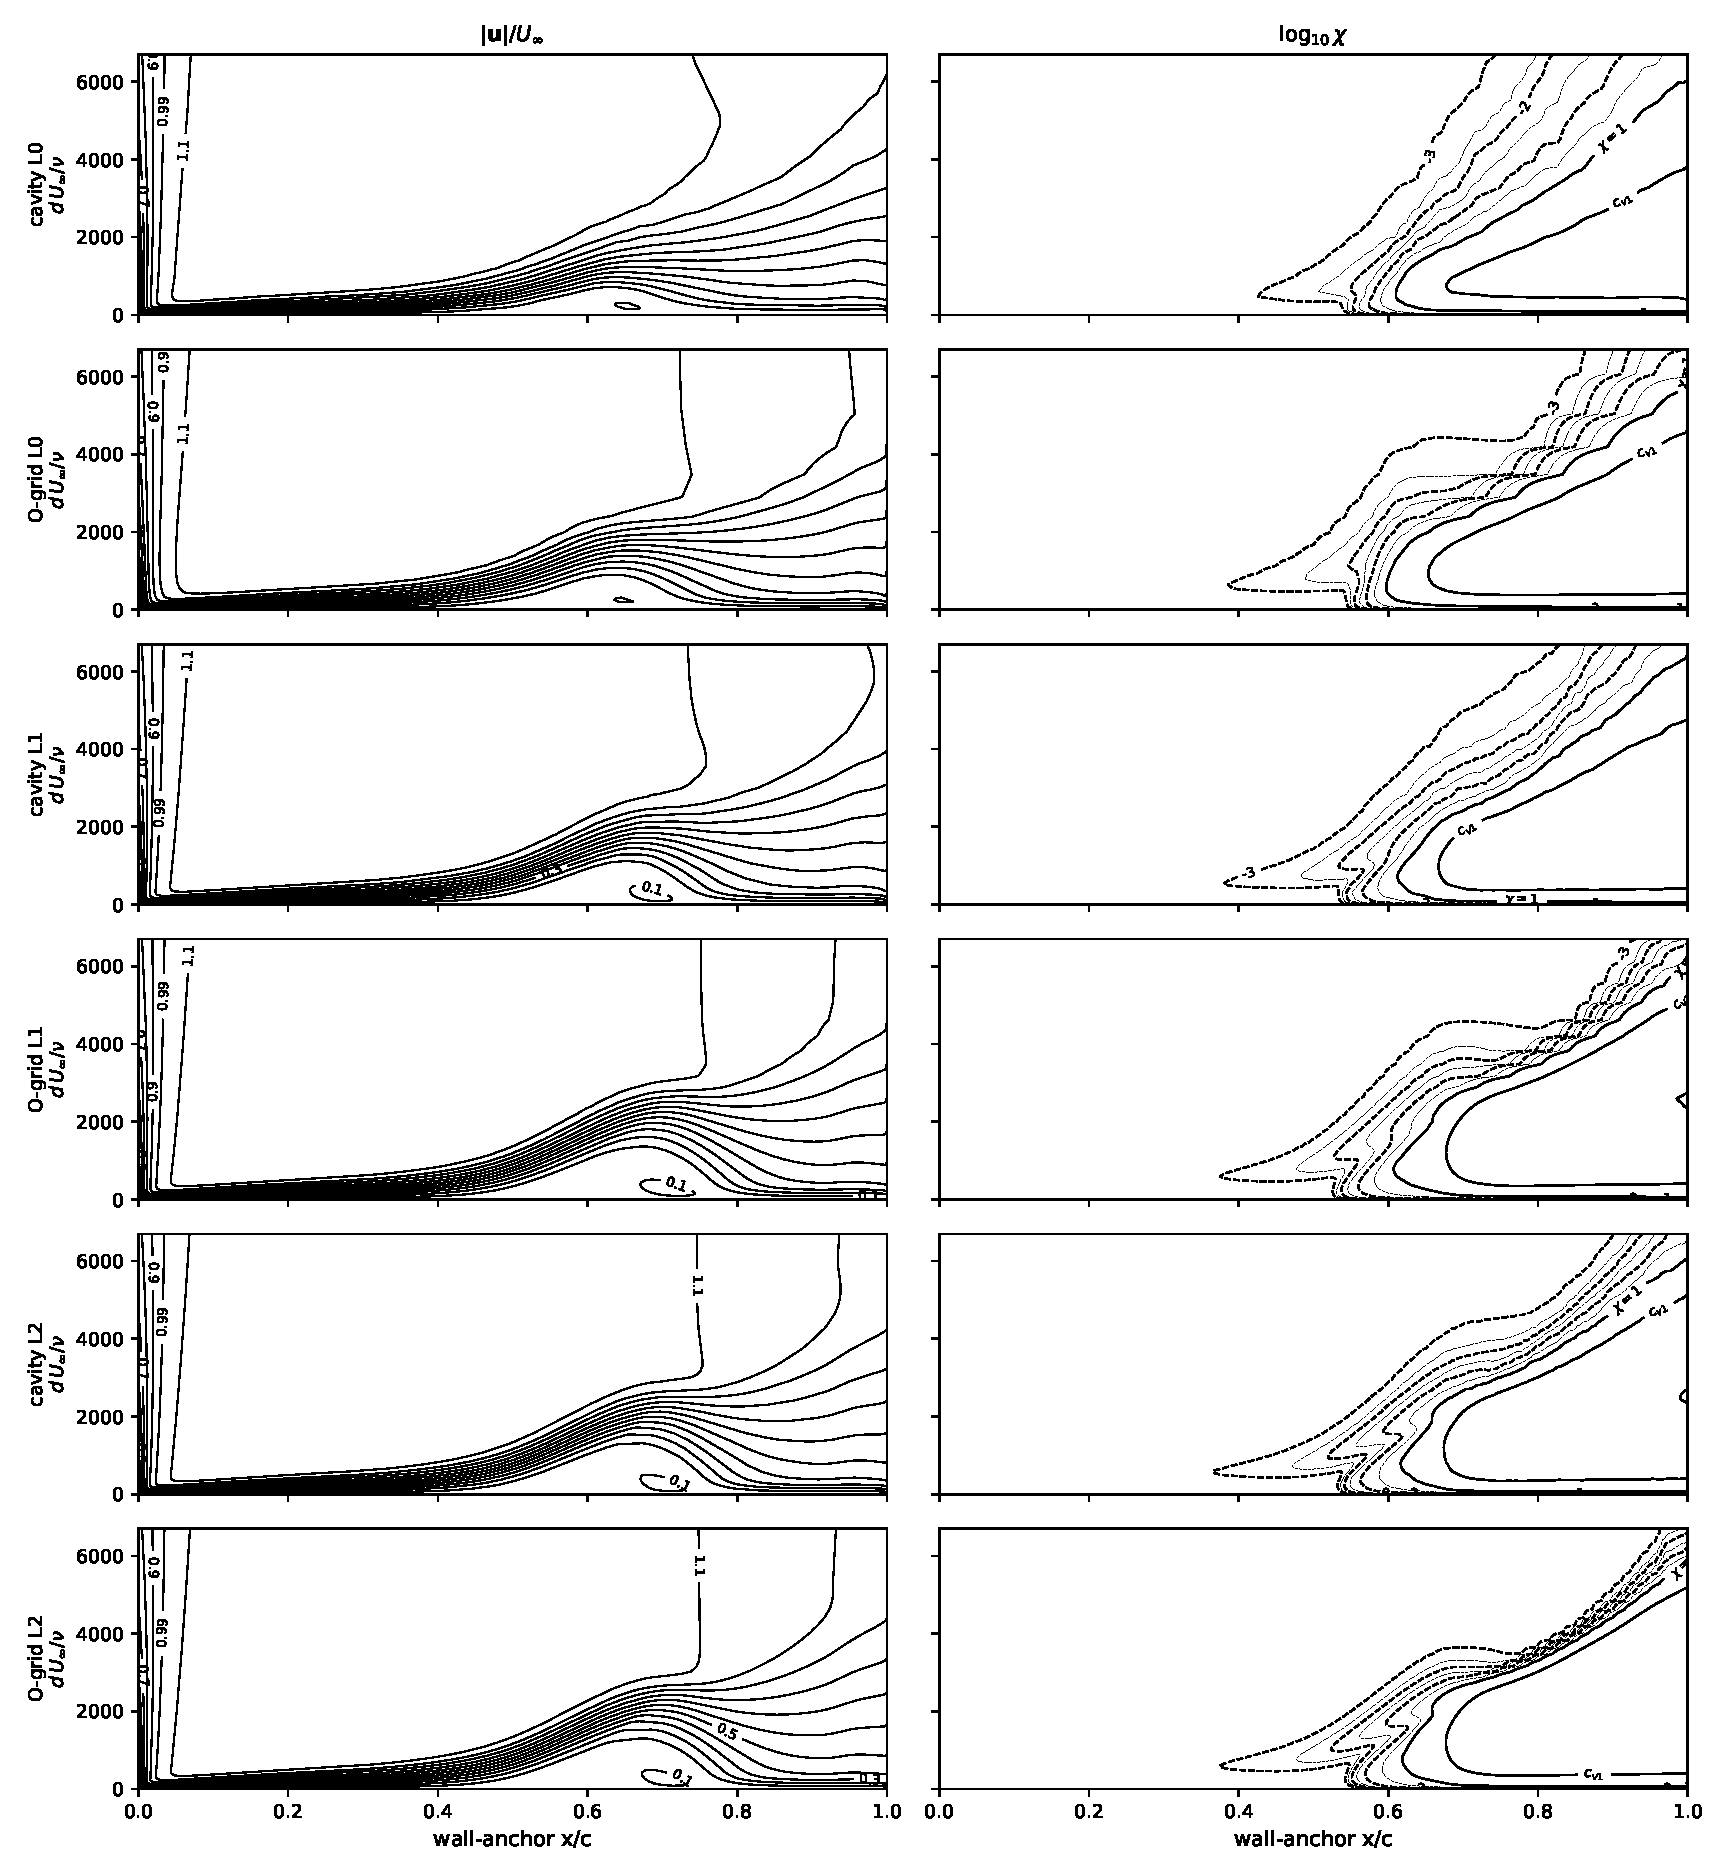
\includegraphics[width=0.99\textwidth]{chi_sheet_eppler387_a0_upper.pdf}
  \caption{Eppler~387, $Re=2\times10^5$, $\alpha=0^\circ$, upper surface: velocity magnitude (left) and $\log_{10}\chi$ (right) on all six grids.}
  \label{fig:sheet_eppler387_a0_upper}
\end{figure}

\begin{figure}[p]
  \centering
  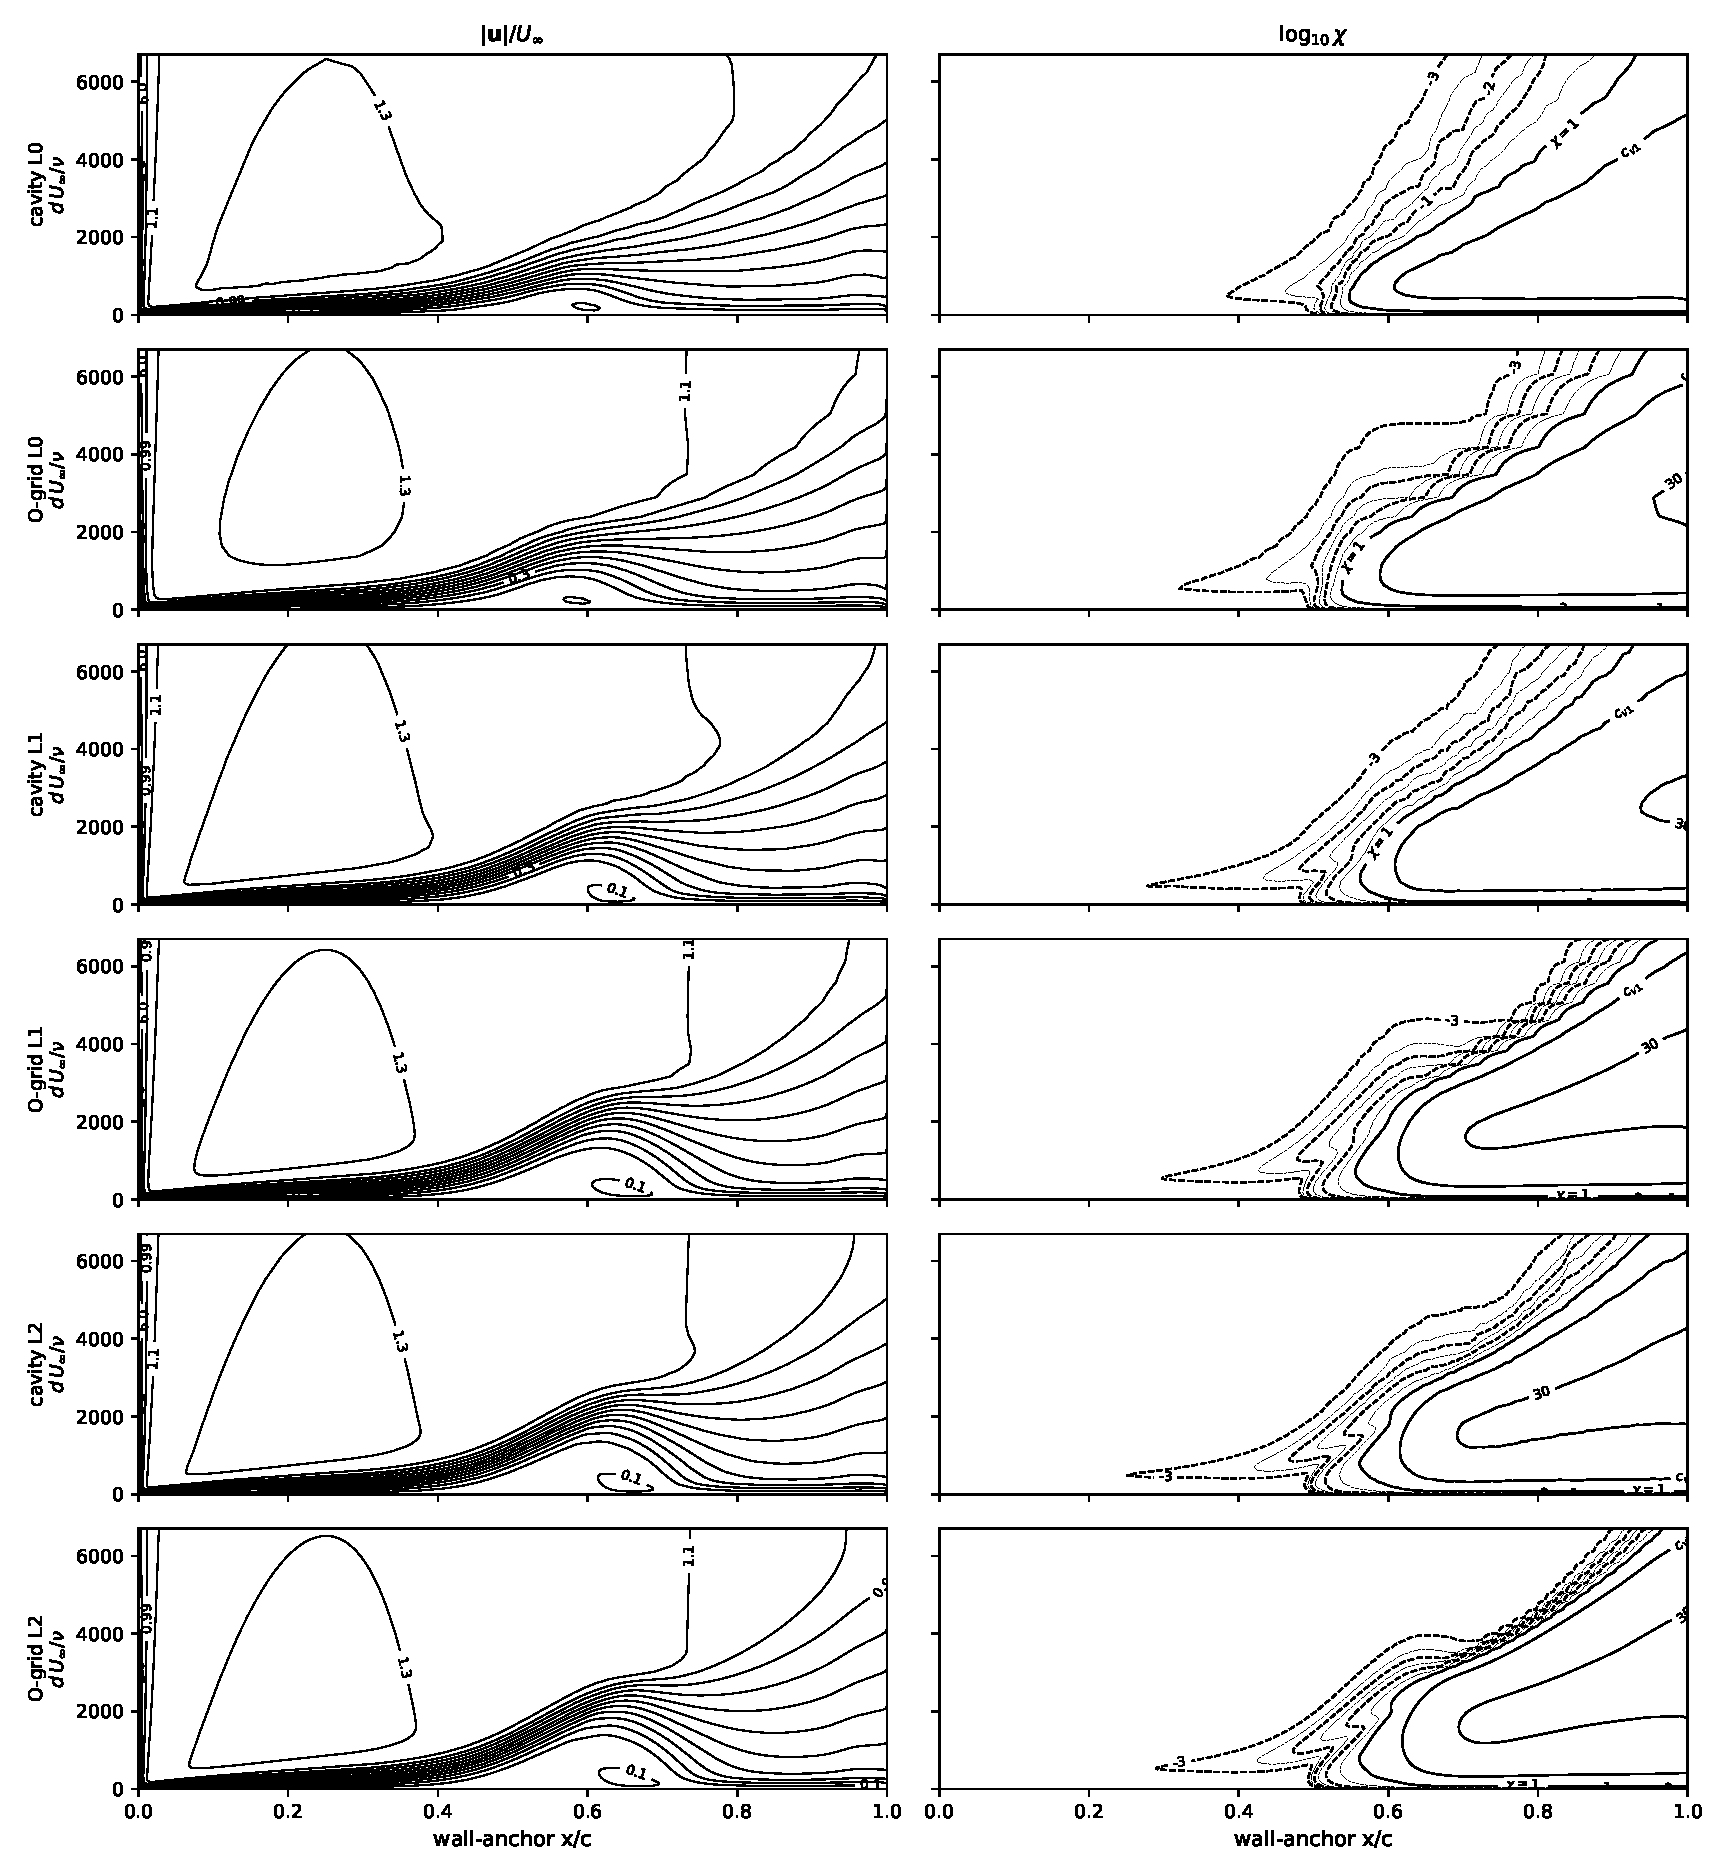
\includegraphics[width=0.99\textwidth]{chi_sheet_eppler387_a2_upper.pdf}
  \caption{Eppler~387, $Re=2\times10^5$, $\alpha=2^\circ$, upper surface: velocity magnitude (left) and $\log_{10}\chi$ (right) on all six grids.}
  \label{fig:sheet_eppler387_a2_upper}
\end{figure}

\begin{figure}[p]
  \centering
  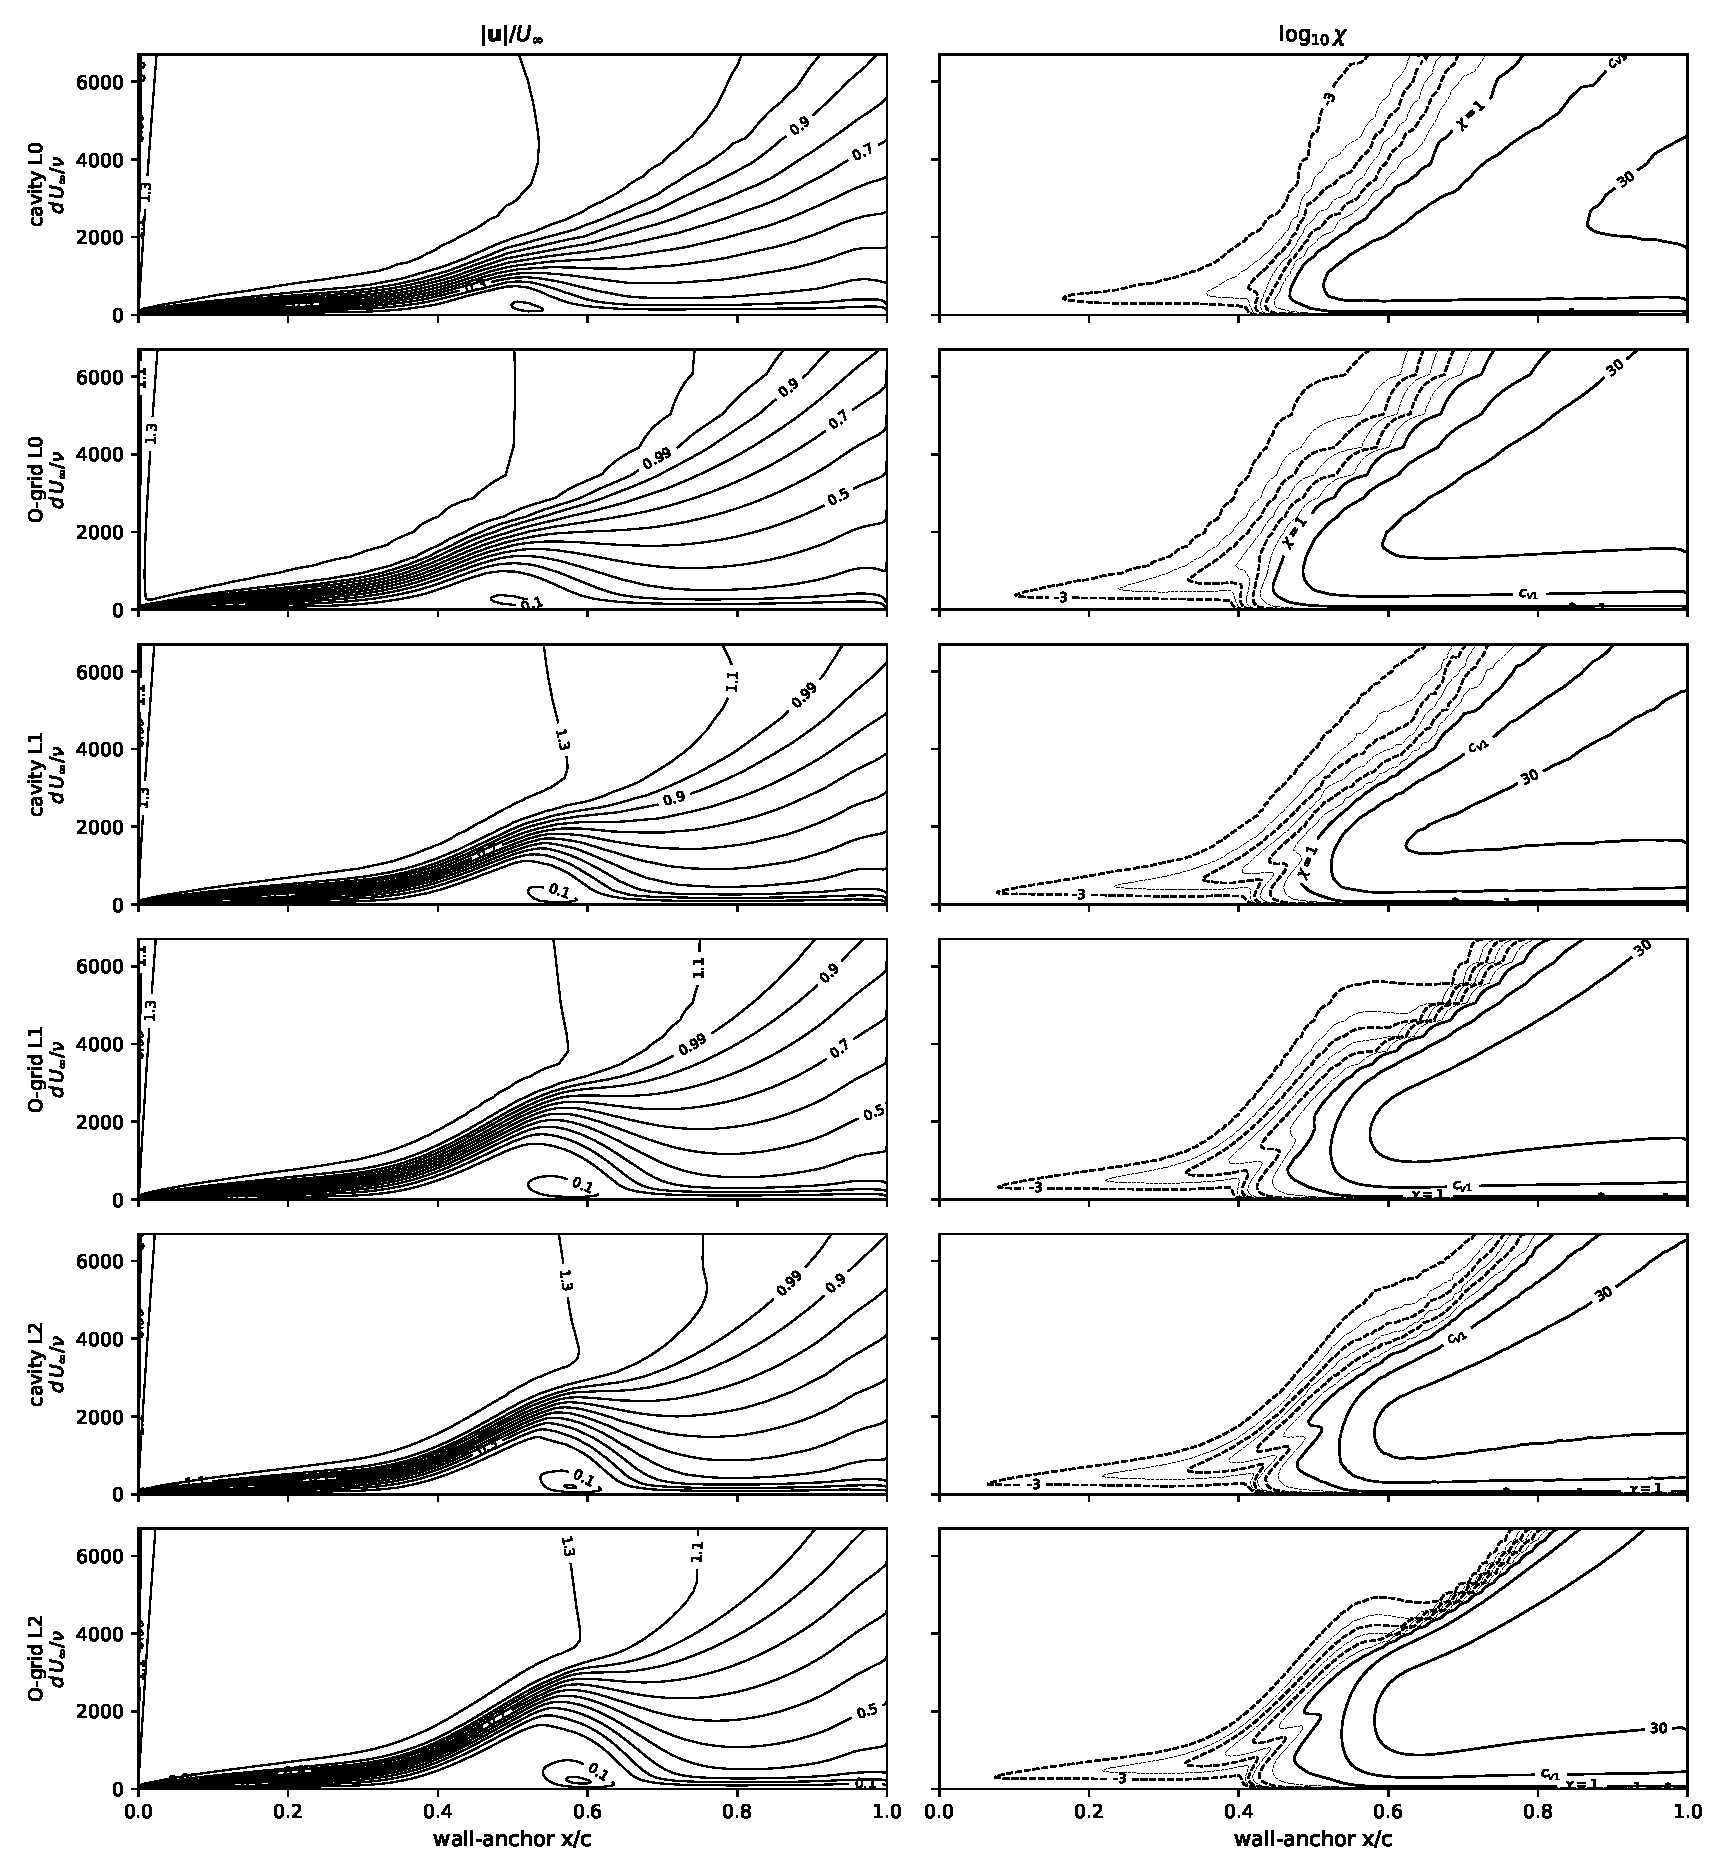
\includegraphics[width=0.99\textwidth]{chi_sheet_eppler387_a5_upper.pdf}
  \caption{Eppler~387, $Re=2\times10^5$, $\alpha=5^\circ$, upper surface: velocity magnitude (left) and $\log_{10}\chi$ (right) on all six grids.}
  \label{fig:sheet_eppler387_a5_upper}
\end{figure}

\begin{figure}[p]
  \centering
  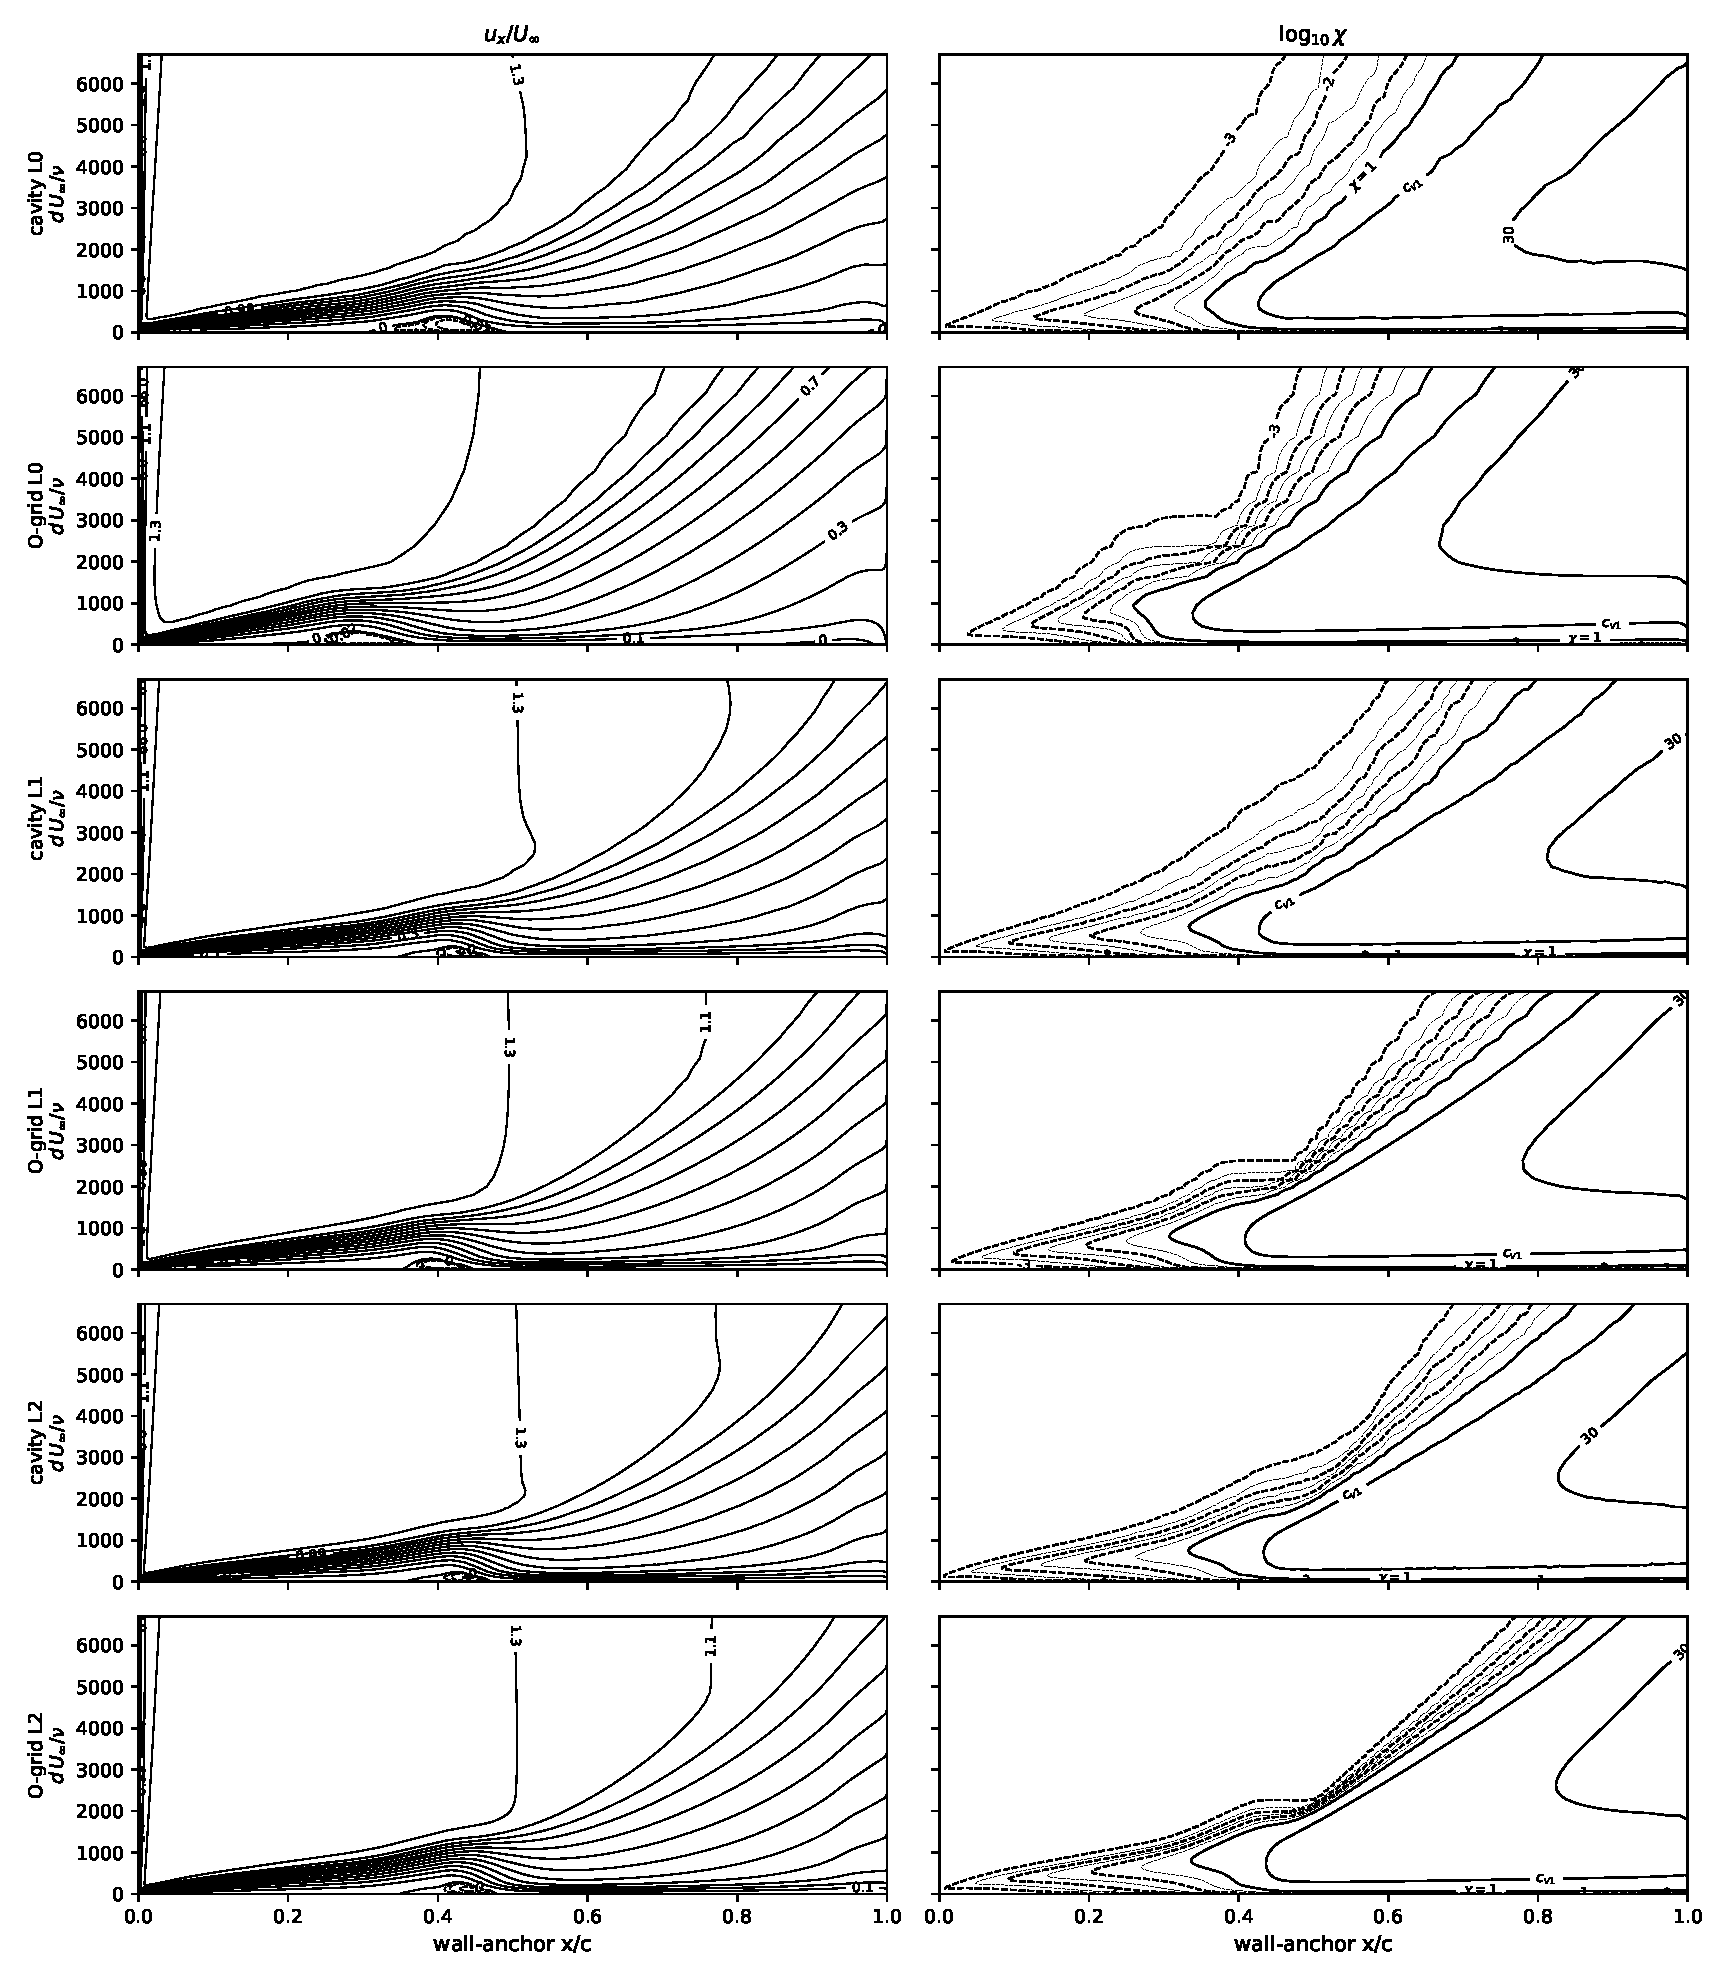
\includegraphics[width=0.99\textwidth]{chi_sheet_eppler387_a7_upper.pdf}
  \caption{Eppler~387, $Re=2\times10^5$, $\alpha=7^\circ$, upper surface: velocity magnitude (left) and $\log_{10}\chi$ (right) on all six grids.}
  \label{fig:sheet_eppler387_a7_upper}
\end{figure}

\begin{figure}[p]
  \centering
  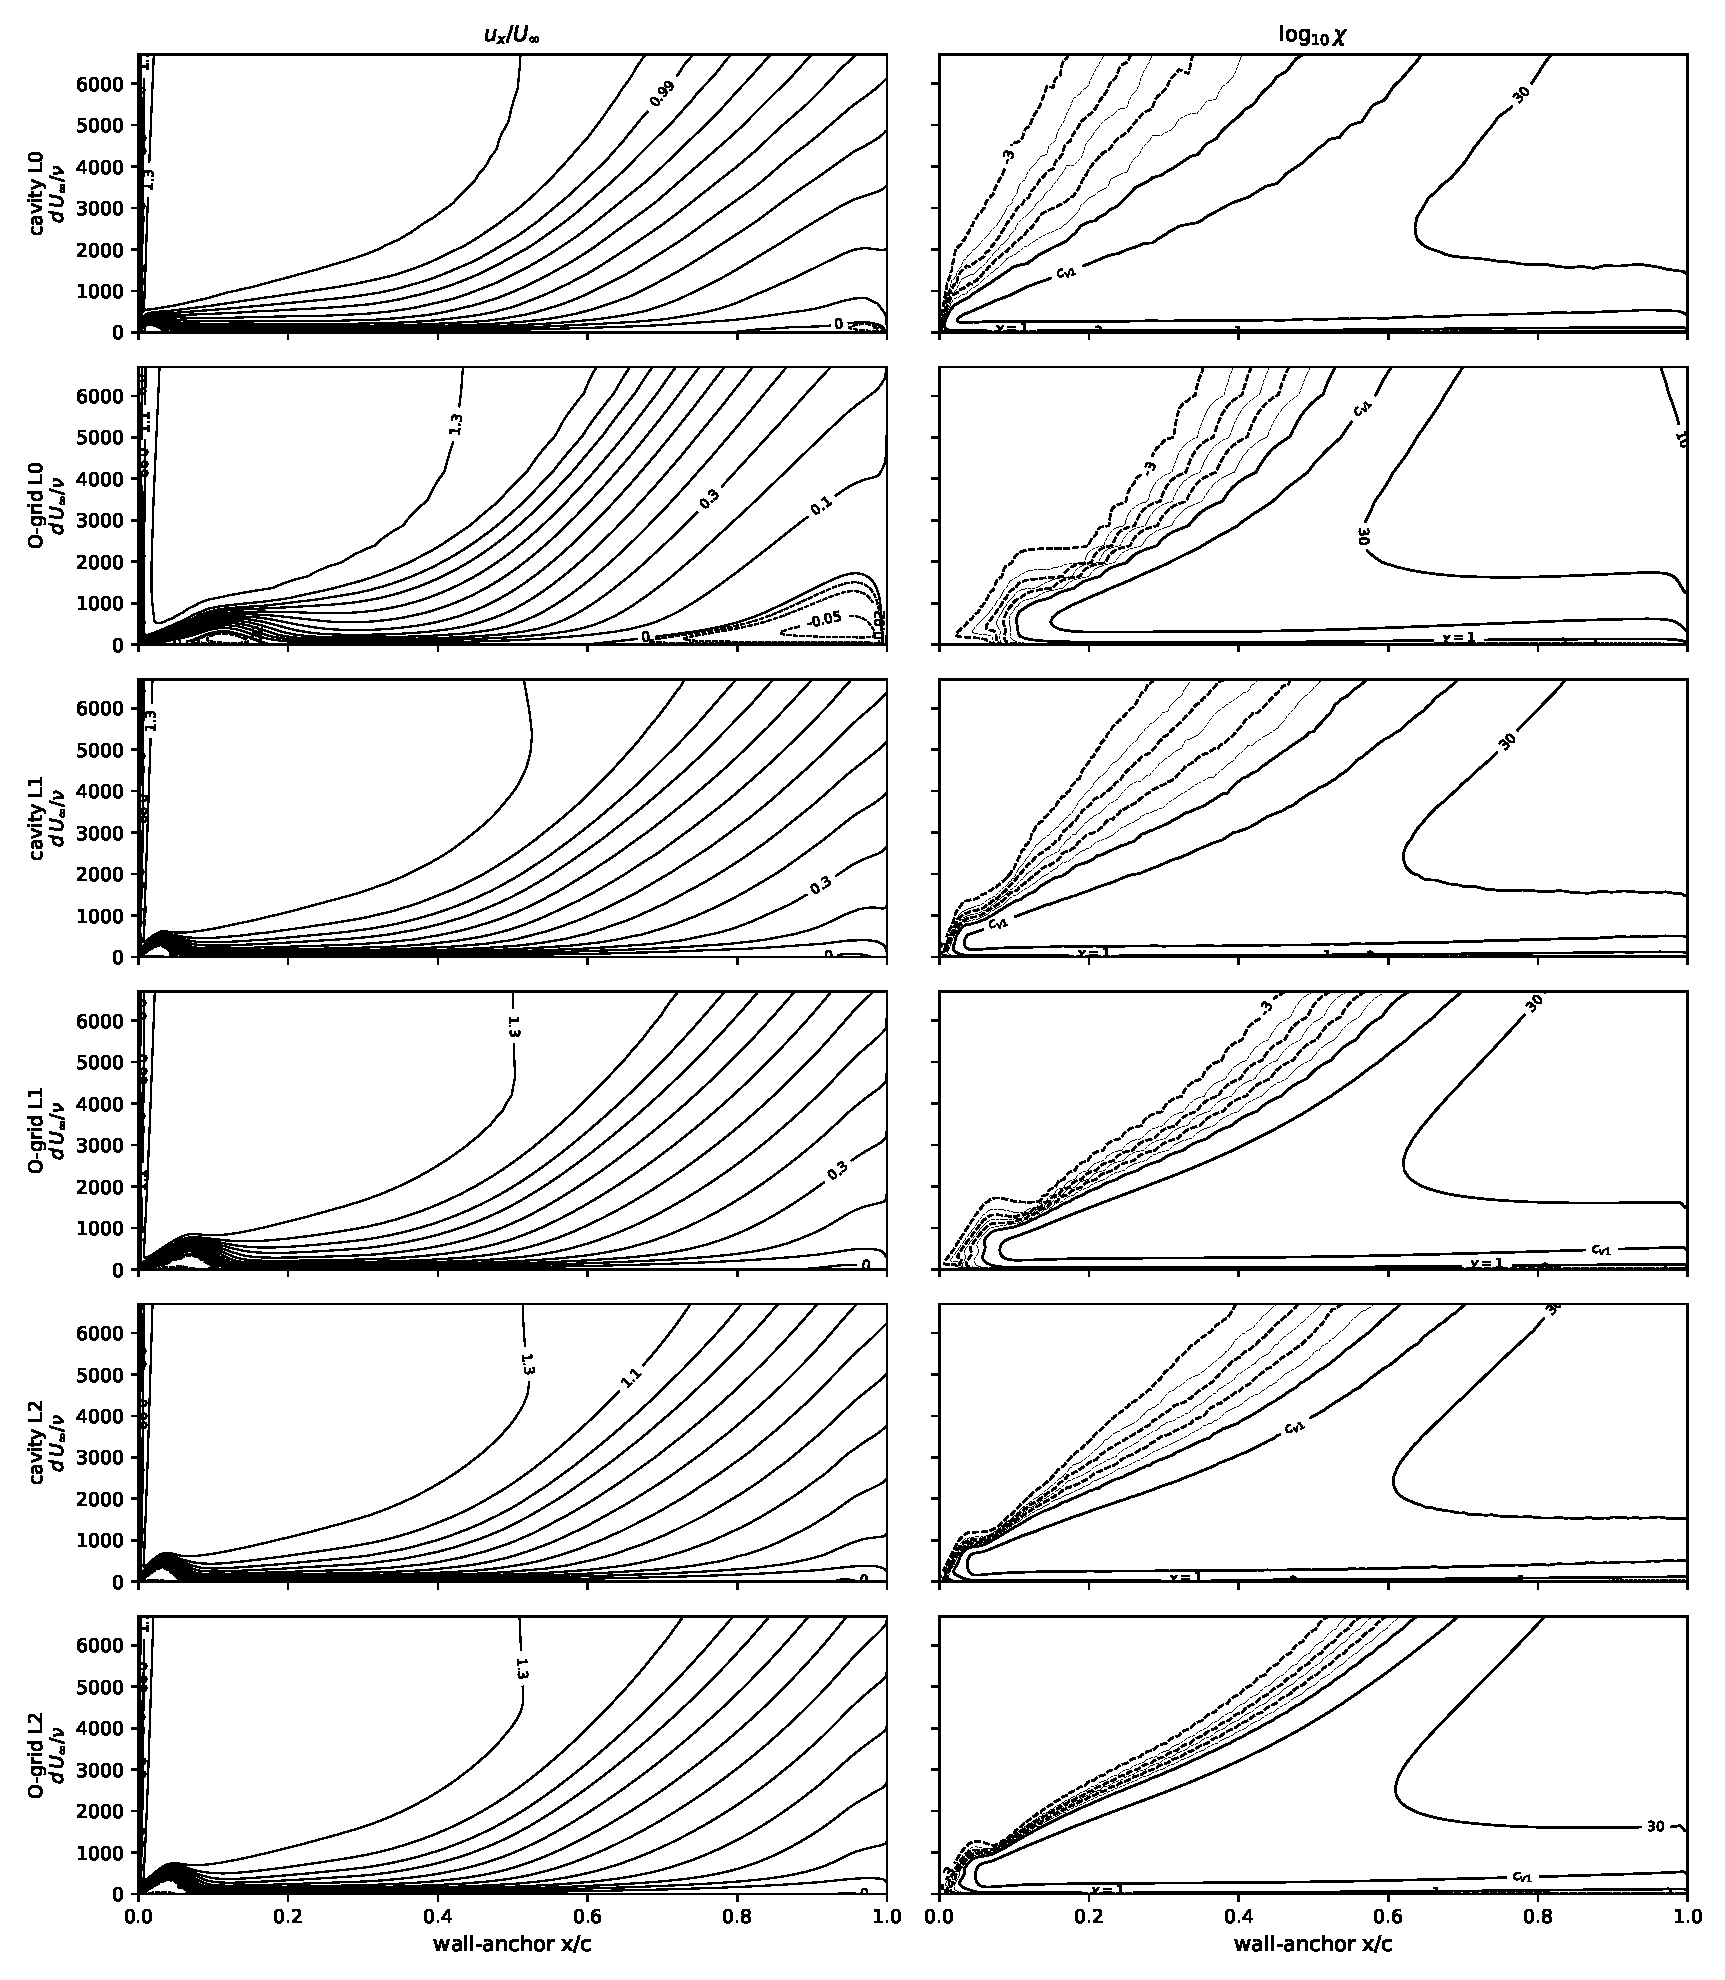
\includegraphics[width=0.99\textwidth]{chi_sheet_eppler387_a8p5_upper.pdf}
  \caption{Eppler~387, $Re=2\times10^5$, $\alpha=8.5^\circ$, upper
  surface (finest L2 pair): velocity magnitude (left) and
  $\log_{10}\chi$ (right). Post-stall: the layer trips in the
  leading-edge bubble within the first few percent of chord
  (Fig.~\ref{fig:eppcfhigh}) and runs turbulent and attached over the
  rest of the surface.}
  \label{fig:sheet_eppler387_a8p5_upper}
\end{figure}

\clearpage
\renewcommand{\thefigure}{C\arabic{figure}}
\renewcommand{\thetable}{C\arabic{table}}
\setcounter{figure}{0}\setcounter{table}{0}
\section*{Appendix C: the Eppler 387 Reynolds sweep---contour sheets}

One upper-surface sheet per swept Reynolds number of
Sec.~\ref{sec:eppresweep} (the $Re=2\times10^5$ anchor is the
$\alpha\!=\!5^\circ$ sheet of Appendix~B), each covering the full
L0--L2 suite on both mesh families; the wall-normal frame scales as
$\smash{\sqrt{2\times10^5/Re}}$. At $Re=10^5$ two additional rows
show each family's warm-started L2 solution after its
$40\,000$-iteration extension (Sec.~\ref{sec:eppbistab}): the fields
agree with the cold-start L2 rows above them to within the cavity
family's residual unsteadiness---the initialization independence of
the converged state, seen in the field variables.
Table~\ref{tab:eppresweep} tabulates the sweep's L2 section
coefficients against the $e^9$ reference and the tunnel data
(discussed in Sec.~\ref{sec:eppresweep}).

\begin{table}[tp]
  \centering
  \small
  \setlength{\tabcolsep}{4.5pt}
  \caption{Section coefficients for the Eppler 387 at $\alpha\!=\!5^\circ$
  across the Reynolds sweep: lift, drag, and quarter-chord pitching moment from
  the two mesh families' finest (L2) grids (the same grids as the
  $Re\!=\!2\!\times\!10^5$ study; the L0/L1 companions appear in
  Figs.~\ref{fig:eppresweep_low}--\ref{fig:eppresweep_high}
  and~\ref{fig:eppresweepforces}). The families' L2 drags agree to
  $0.1$--$0.2\!\times\!10^{-3}$ at $2$--$4.6\!\times\!10^5$ and diverge
  at $10^5$ as described in the text; the $10^5$ states are
  initialization-independent (Sec.~\ref{sec:eppbistab}). Also listed: the $e^9$ panel reference (mfoil; XFOIL at $6\!\times\!10^4$,
  where the two implementations visibly differ, and at
  $Re\!=\!4.6\!\times\!10^5$, where mfoil's stagnation-point iteration
  diverges on the thin high-$Re$ bubble), and the LTPT measurement
  (McGhee et al., NASA TM-4062,
  Table~B1, read at the tabulated angle nearest $5^\circ$:
  $\alpha\!=\!4.99^\circ$--$5.06^\circ$). The computed moment is transferred
  from the solver's leading-edge reference to the quarter chord,
  $c_m\!=\!c_{m,\mathrm{LE}}+\tfrac14(c_l\cos\alpha+c_d\sin\alpha)$. Repeat
  experimental points at $Re\!\geq\!10^5$ agree to within $0.006$ in $c_l$ and
  $0.0003$ in $c_d$; at $Re\!=\!6\!\times\!10^4$ the flow is bistable and the
  repeat scatter is an order of magnitude larger (see text).}
  \label{tab:eppresweep}
  \begin{tabular}{l ccc ccc ccc ccc}
    \toprule
    & \multicolumn{3}{c}{SA-AI, structured L2} & \multicolumn{3}{c}{SA-AI, unstructured L2}
    & \multicolumn{3}{c}{$e^9$ panel} & \multicolumn{3}{c}{Exp (LTPT)}\\
    \cmidrule(lr){2-4}\cmidrule(lr){5-7}\cmidrule(lr){8-10}\cmidrule(lr){11-13}
    $Re$ & $c_l$ & $c_d$ & $c_m$ & $c_l$ & $c_d$ & $c_m$ & $c_l$ & $c_d$ & $c_m$ & $c_l$ & $c_d$ & $c_m$ \\
    \midrule
    $6\!\times\!10^4$   & 0.636 & 0.0533 & $-$0.098 & 0.712 & 0.0506 & $-$0.103 & 0.869$^\ddagger$ & 0.0411$^\ddagger$ & $-$0.102$^\ddagger$ & 0.838 & 0.0439 & $-$0.114 \\
    $1\!\times\!10^5$   & 0.795 & 0.0410 & $-$0.102 & 0.877 & 0.0307 & $-$0.096 & 0.952 & 0.0213 & $-$0.087 & 0.873 & 0.0237 & $-$0.089 \\
    $2\!\times\!10^5$   & 0.927 & 0.0145 & $-$0.081 & 0.938 & 0.0143 & $-$0.083 & 0.960 & 0.0128 & $-$0.082 & 0.891 & 0.0138 & $-$0.081 \\
    $3\!\times\!10^5$   & 0.941 & 0.0107 & $-$0.080 & 0.950 & 0.0108 & $-$0.082 & 0.962 & 0.0103 & $-$0.082 & 0.901 & 0.0114 & $-$0.080 \\
    $4.6\!\times\!10^5$ & 0.950 & 0.0087 & $-$0.081 & 0.959 & 0.0089 & $-$0.083 & 0.966 & 0.0086 & $-$0.082 & 0.914 & 0.0093 & $-$0.081 \\
    \bottomrule
  \end{tabular}
  \\[2pt]{\footnotesize $^\ddagger$The only condition in this paper where
  the $e^9$ implementations visibly differ; XFOIL, whose forces sit
  closer to the measurement, is quoted as the reference. mfoil gives
  $c_l\!=\!0.889$, $c_d\!=\!0.0368$, $c_m\!=\!-0.097$---$11\%$ less
  drag---commensurate with the bistability of the flow at this Reynolds
  number, while a third, separately written implementation of the
  XFOIL closure set (FlexFoil, Flexcompute's Rust reimplementation)
  sides with XFOIL: $c_l\!=\!0.868$, $c_d\!=\!0.0406$,
  $c_m\!=\!-0.102$. At every other condition (both airfoils, all
  incidences, the higher Reynolds numbers, and the wing sections of
  Sec.~\ref{sec:daedalus}) all three agree to better than $1\%$ in
  $c_l$ and $c_d$, and to $0.005\,c$ in $x_\mathrm{tr}$ with one
  exception: the NLF $\alpha\!=\!0^\circ$ lower-surface front, whose
  near-flat envelope amplifies implementation differences---mfoil and
  FlexFoil both read $0.62\,c$, while an XFOIL run of the original study
  read $0.52\,c$ (Sec.~\ref{sec:nlfval}).}
\end{table}

\begin{figure}[p]
  \centering
  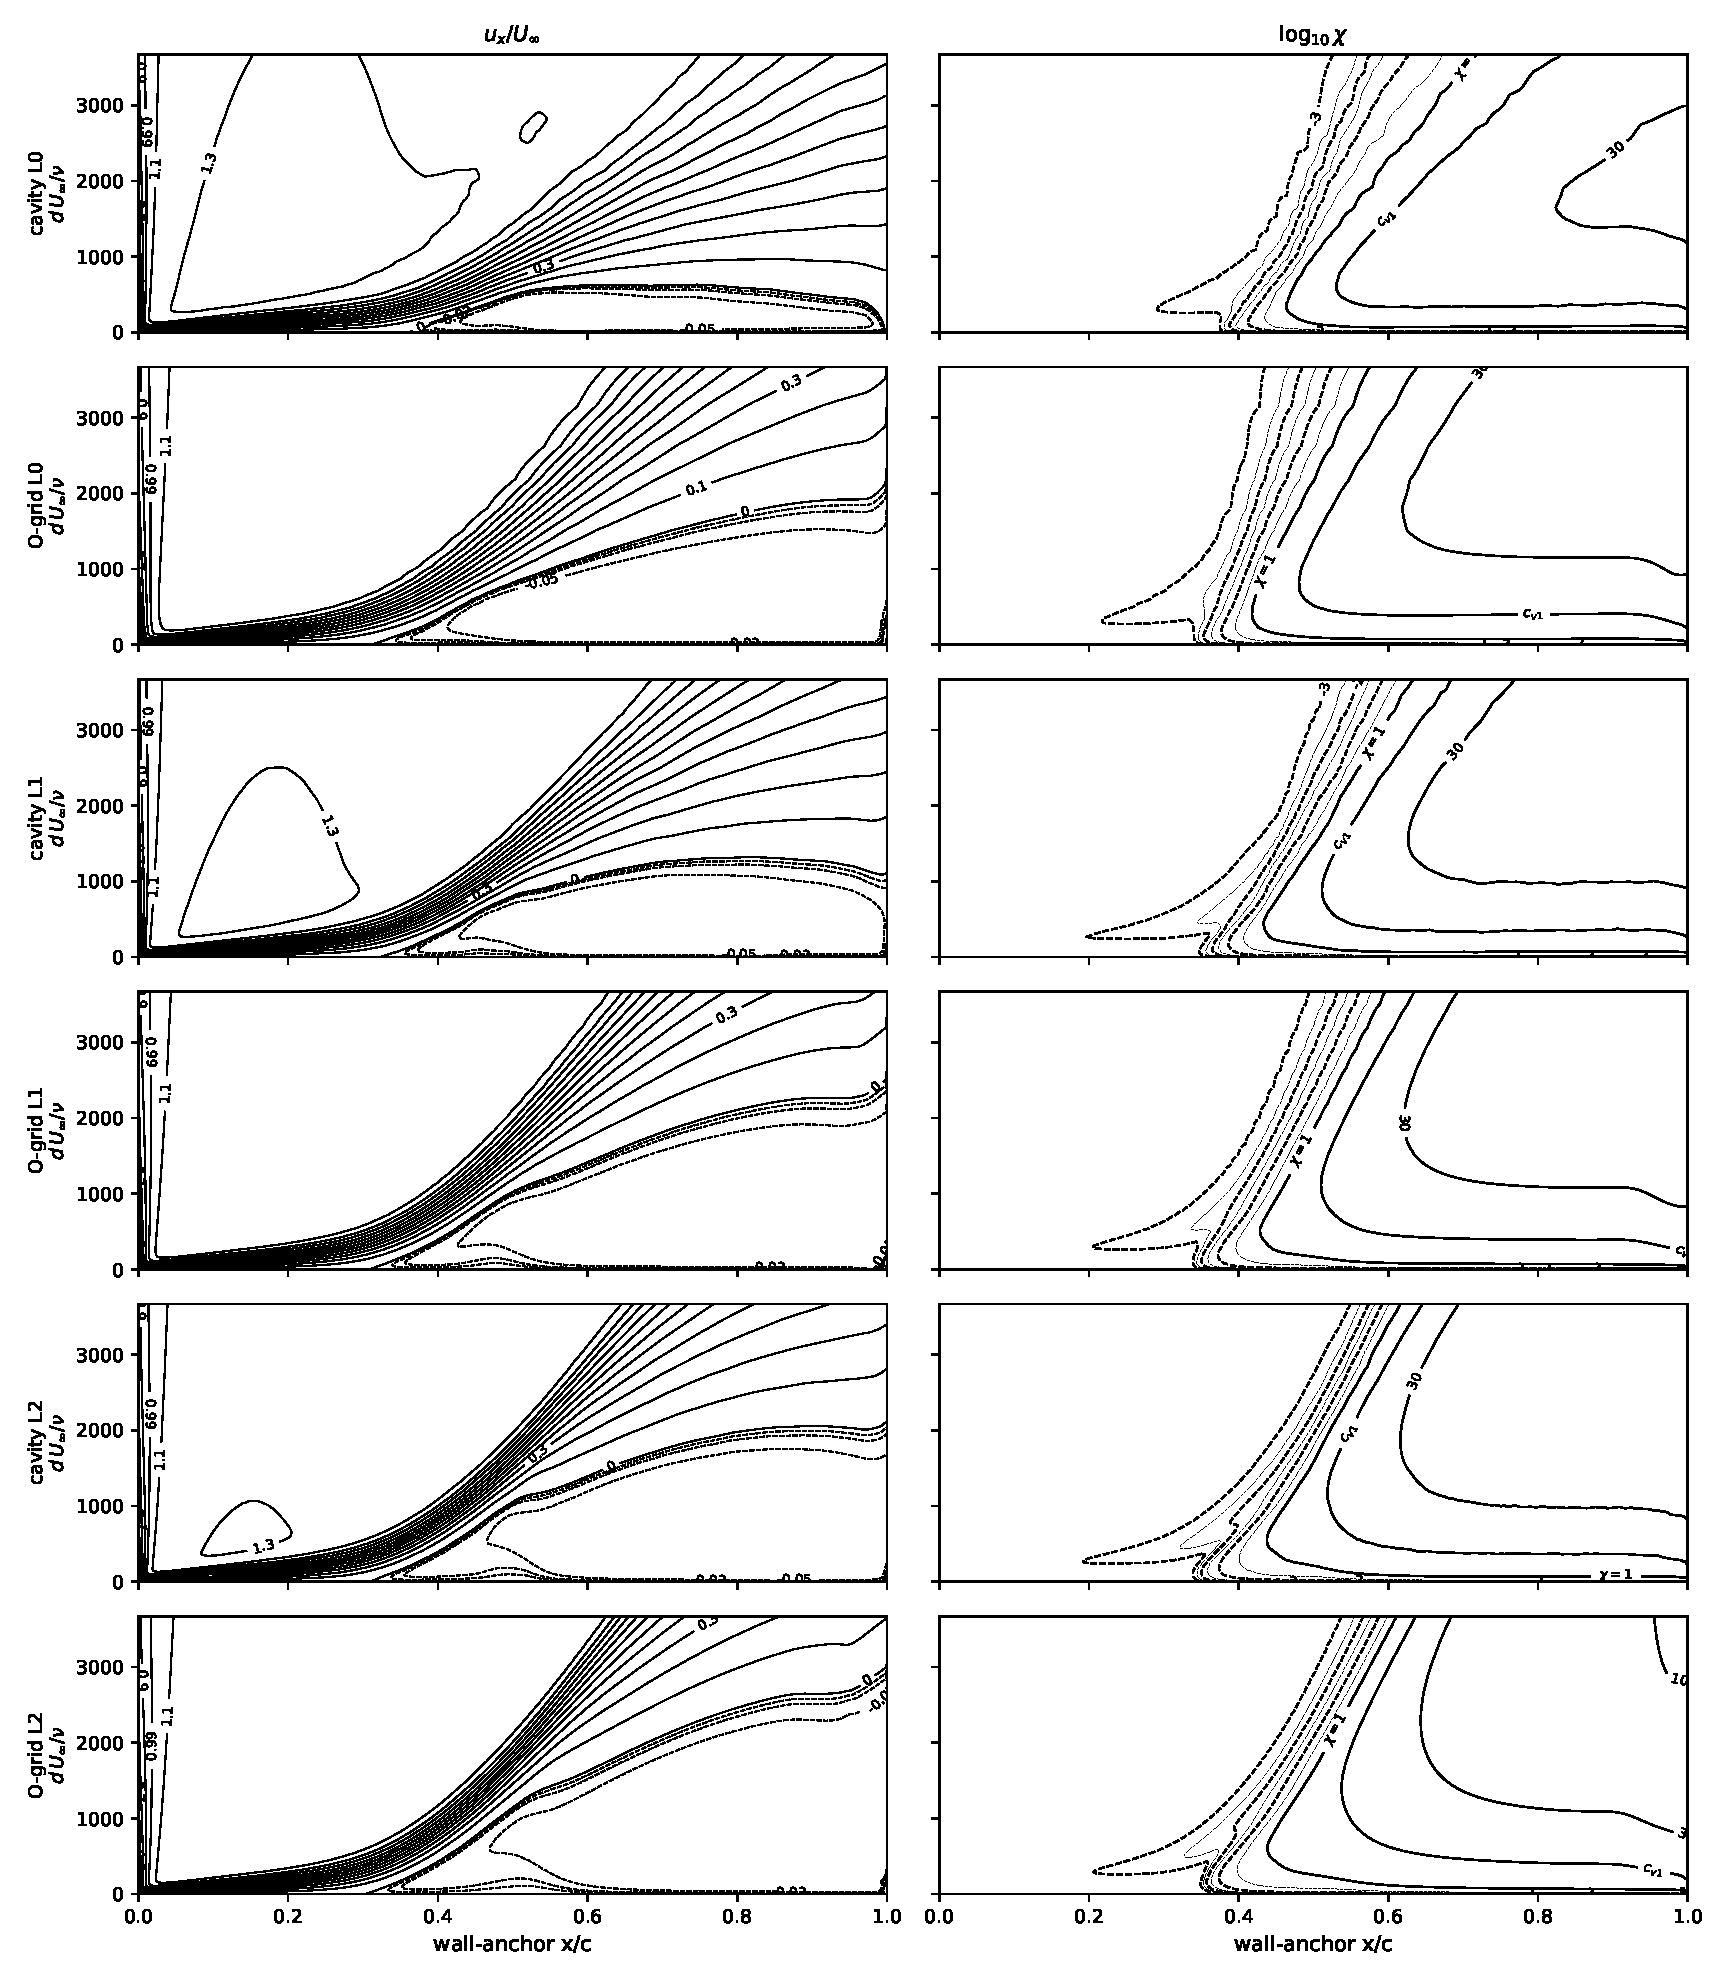
\includegraphics[width=0.99\textwidth]{chi_sheet_eppler387_Re60k_upper.pdf}
  \caption{Eppler~387, $Re=6\times10^4$, $\alpha=5^\circ$, upper surface: velocity magnitude (left) and $\log_{10}\chi$ (right) on all six grids.}
  \label{fig:sheet_eppler387_Re60k_upper}
\end{figure}

\begin{figure}[p]
  \centering
  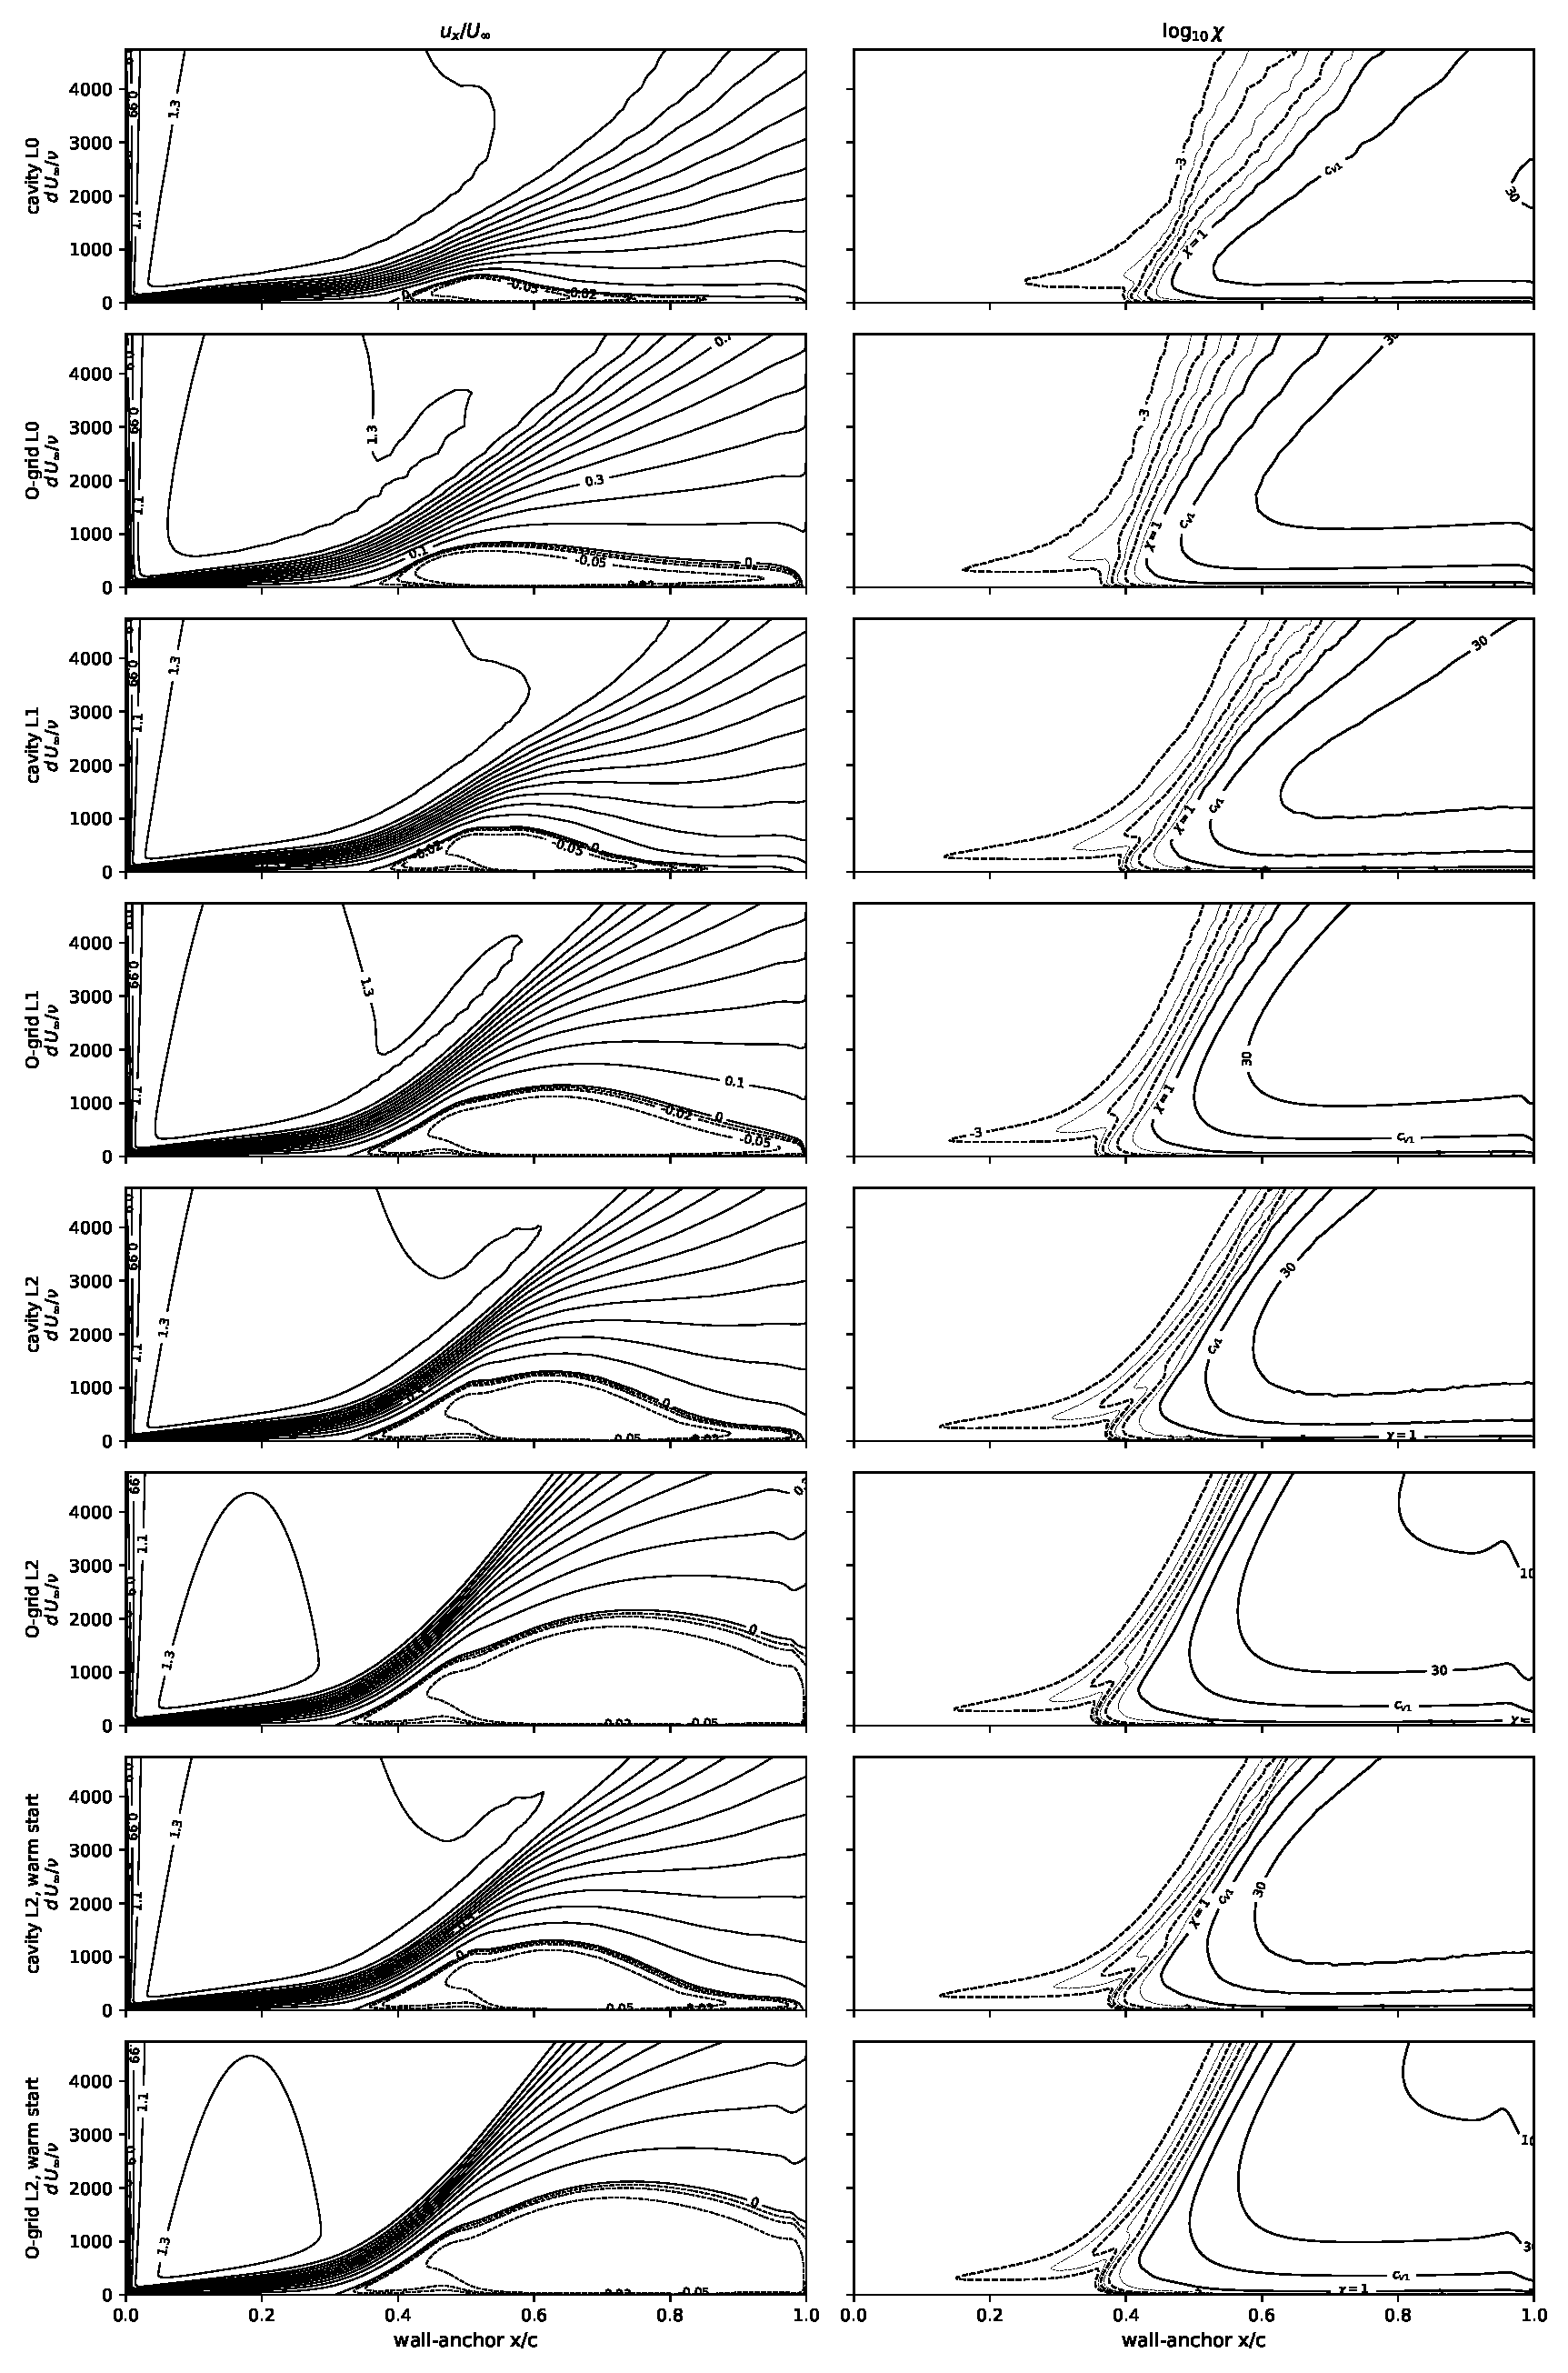
\includegraphics[width=0.82\textwidth]{chi_sheet_eppler387_Re100k_upper.pdf}
  \caption{Eppler~387, $Re=10^5$, $\alpha=5^\circ$, upper surface, all six
  grids plus the two extended warm-started L2 solutions (bottom rows),
  agreeing with the cold-start L2 rows to within the residual
  unsteadiness (Sec.~\ref{sec:eppbistab}).}
  \label{fig:sheet_eppler387_Re100k_upper}
\end{figure}

\begin{figure}[p]
  \centering
  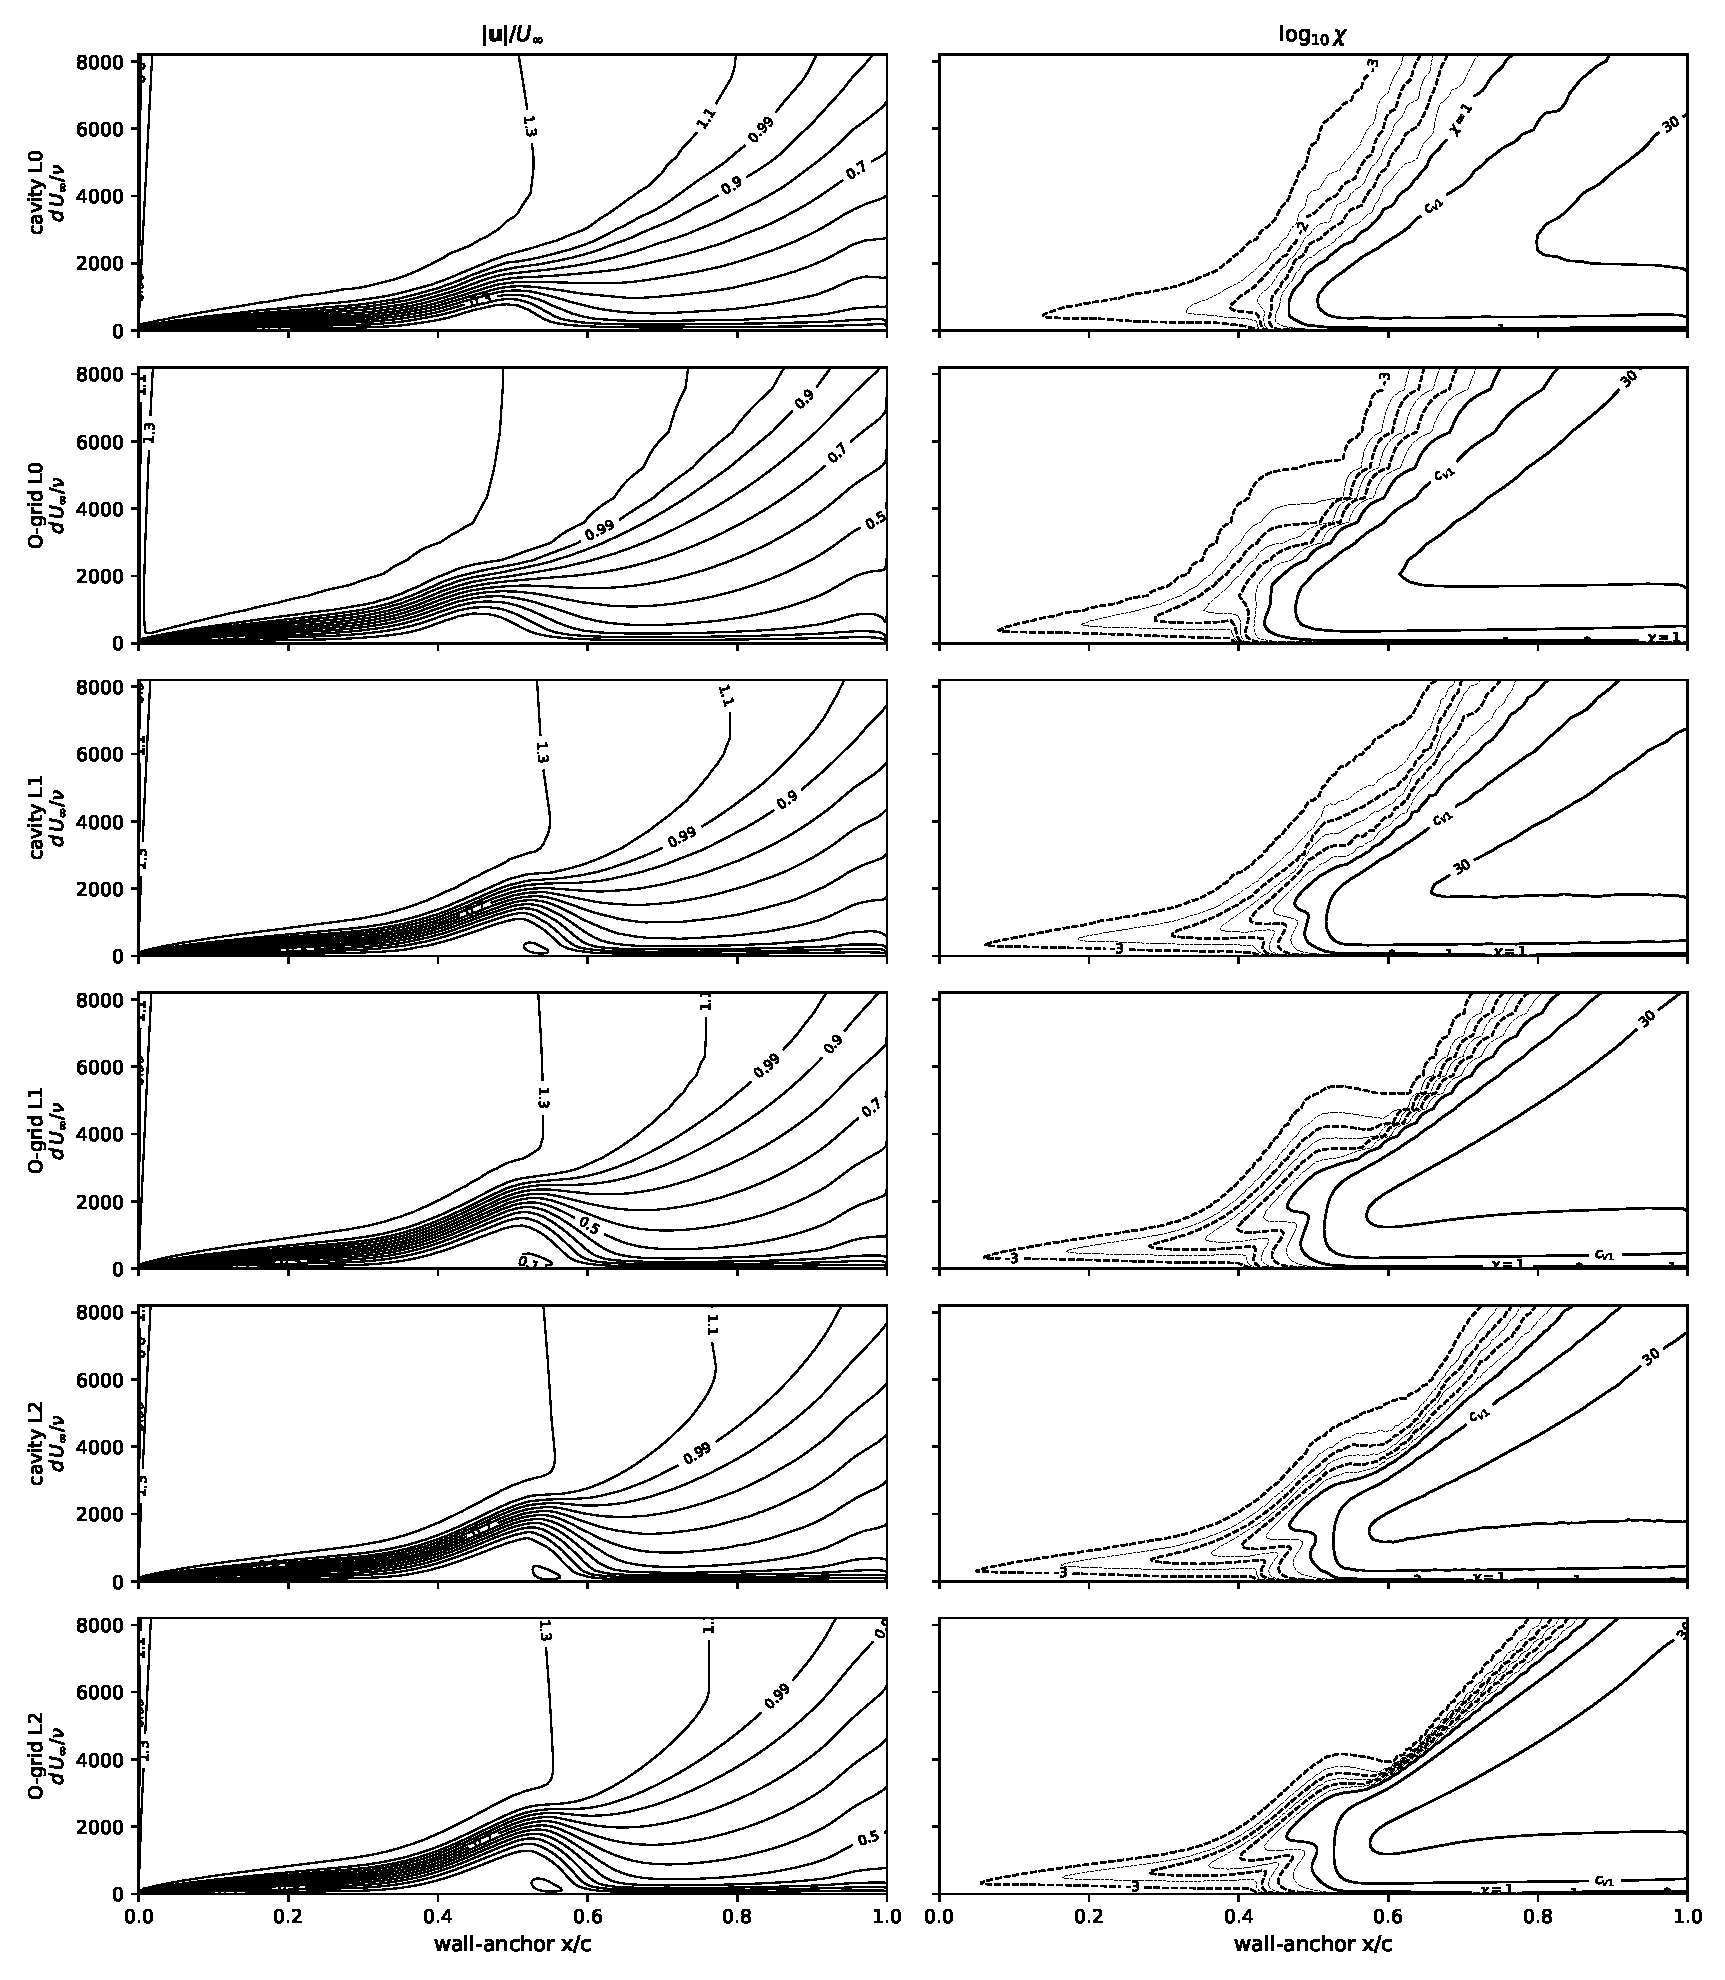
\includegraphics[width=0.99\textwidth]{chi_sheet_eppler387_Re300k_upper.pdf}
  \caption{Eppler~387, $Re=3\times10^5$, $\alpha=5^\circ$, upper surface: velocity magnitude (left) and $\log_{10}\chi$ (right) on all six grids.}
  \label{fig:sheet_eppler387_Re300k_upper}
\end{figure}

\begin{figure}[p]
  \centering
  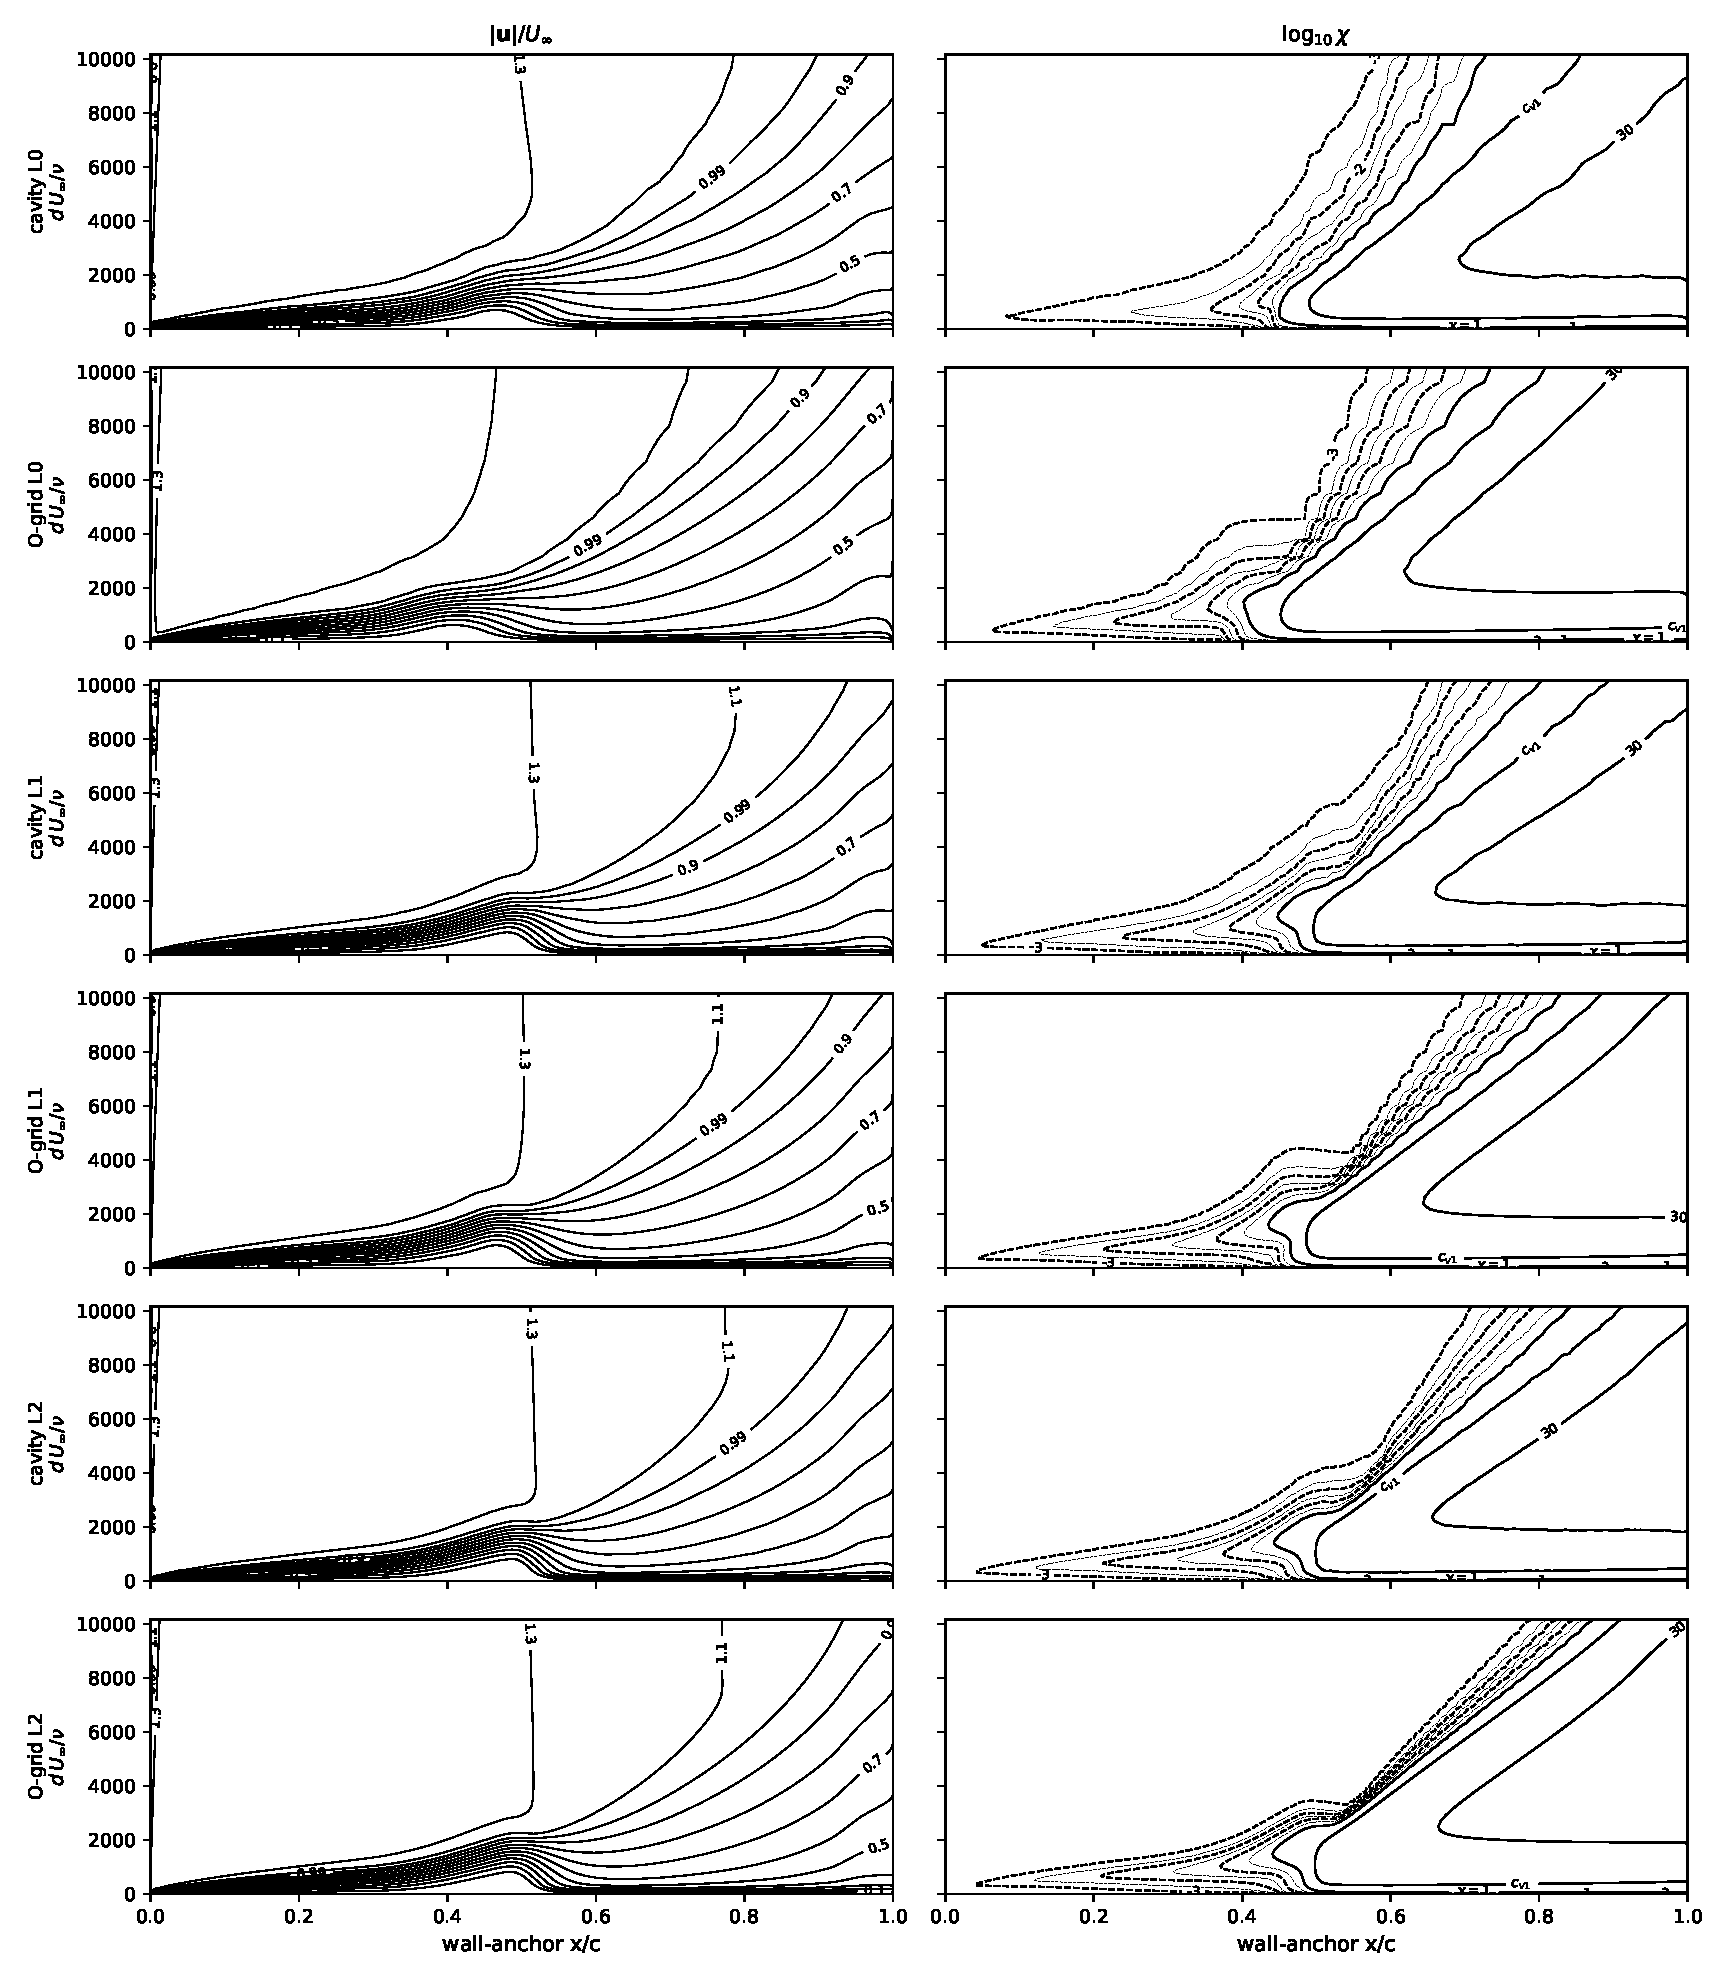
\includegraphics[width=0.99\textwidth]{chi_sheet_eppler387_Re460k_upper.pdf}
  \caption{Eppler~387, $Re=4.6\times10^5$, $\alpha=5^\circ$, upper surface: velocity magnitude (left) and $\log_{10}\chi$ (right) on all six grids.}
  \label{fig:sheet_eppler387_Re460k_upper}
\end{figure}

\clearpage
\renewcommand{\thefigure}{D\arabic{figure}}
\renewcommand{\thetable}{D\arabic{table}}
\setcounter{figure}{0}\setcounter{table}{0}
\section*{Appendix D: the Daedalus wing---definition, temporal-units
conversion, and force tables}

\paragraph{Geometry, meshes, and solutions.} The wing blends the
DAE-11, DAE-21, and DAE-31 sections~\cite{drela_daedalus_1988} along
the span (transition stations $\eta\!=\!0.30$ and $0.60$), holds the
$0.917\,$m chord to $\eta\!=\!0.88$, and tapers linearly to $0.35\,$m
at the tip with a straight quarter-chord line. The structured family
stacks two-dimensional O-grids spanwise, pinching the section to a line
beyond the tip. The unstructured family is a classical
three-dimensional unstructured mesh, distinct from the two-dimensional
cavity construction of Appendices~A and~B: anisotropic boundary-layer prisms
are grown from the triangulated wing surface, the far field is an
octree of hexahedra, and tetrahedra join the two, with the tetrahedron
size at the interface seeded from the area-equivalent edge length of
the surface triangles and the prism stack terminated where its height
reaches the local isotropic scale. Sizes, spanwise-station and
around-the-section resolution are tabulated in the main text
(Table~\ref{tab:daemesh}). All solutions use the airfoil-study solver
settings with the final kernel (the recomputation noted at the opening
of Sec.~\ref{sec:daedalus}; the completed set is the one tabulated in
Table~\ref{tab:daetotals}, dashes marking runs in progress) and are
converged to steady or small-limit-cycle force histories; tabulated
coefficients are means over the final 500 pseudo-steps (51 logged
samples).

\begin{table}[tp]
  \centering
  \small
  \caption{Daedalus wing totals by grid level: SA-AI on both mesh
  families against the AVL$+$XFOIL reference trimmed to the RANS lift
  (finest completed level) at each incidence: Trefftz-plane induced
  drag at the trim plus XFOIL profile drag at the trimmed strip
  loading, matched local $c_l$ and $N_\mathrm{crit}\!=\!13.6$,
  integrated over span
  (\texttt{daedalus/avl\_fixed\_cl\_reference.py}). Dashes: runs of
  the final-kernel recomputation still in progress.}
  \label{tab:daetotals}
  \begin{tabular}{cl cc cc}
    \toprule
    & & \multicolumn{2}{c}{structured O-grid} & \multicolumn{2}{c}{unstructured}\\
    \cmidrule(lr){3-4}\cmidrule(lr){5-6}
    $\alpha$ & level & $C_L$ & $C_D$ & $C_L$ & $C_D$\\
    \midrule
    $4^\circ$ & L1 & 1.0278 & 0.01957 & 1.0211 & 0.01975\\
              & L2 & 1.0282 & 0.01997 & 1.0208 & 0.02004\\
              & AVL$+$XFOIL & 1.0282 & 0.02125 & &\\
    \midrule
    $5^\circ$ & L1 & 1.1300 & 0.02212 & 1.1225 & 0.02235\\
              & L2 & 1.1289 & 0.02243 & 1.1223 & 0.02254\\
              & AVL$+$XFOIL & 1.1289 & 0.02315 & &\\
    \midrule
    $6^\circ$ & L1 & 1.2317 & 0.02479 & 1.2227 & 0.02523\\
              & L2 & 1.2279 & 0.02509 & --- & ---\\
              & AVL$+$XFOIL & 1.2279 & 0.02530 & &\\
    \bottomrule
  \end{tabular}
\end{table}

\paragraph{Temporal-units conversion.} The comparisons of
Sec.~\ref{sec:daedalus} and of this appendix's ledger between the kernel
ceiling and the $e^N$ reference convert Drela's envelope slope into a
growth rate per unit time in multiples of the profile's peak vorticity,
\begin{equation*}
  a_\mathrm{eff}
  \;=\;
  \underbrace{\frac{dN}{dRe_\theta}\,\frac{m(H)+1}{2}\,\ell(H)}_{dN/dx\;\cdot\;\theta}
  \;\cdot\;\frac{c/U_e}{\omega_\mathrm{peak}\theta/U_e},
\end{equation*}
with $\ell(H)$ and $m(H)$ the Falkner--Skan similarity factors of
Drela's spatial conversion and $c$ the packet speed, taken as the flow
speed at the profile's inflection point. On the separation-limit
profile ($H\!=\!3.98$: $\theta/\delta_s\!=\!0.585$,
$f''_{\max}\!=\!0.361$, hence
$\omega_\mathrm{peak}\theta/U_e\!=\!0.212$, $c\!=\!0.503\,U_e$) this
gives $a_\mathrm{eff}\!=\!0.066\!=\!0.35\,a_{\max}$: the anchor
condition of the \emph{predecessor} kernel (a shaped, sigmoidal rate;
cf.\ the linear clip of Eq.~\eqref{eq:rate}) pinned its sigmoid's flank at a
third of the ceiling. Profiles extracted from the wing's bubble
(the \emph{predecessor-kernel} campaign's structured L2,
$\eta\!=\!0.31$, $\alpha\!=\!5^\circ$,
$x/c\!=\!0.48$--$0.53$---that kernel's whole bubble; the final-kernel
bubble at the same station spans $0.47$--$0.65\,c$) measure
$\omega_\mathrm{peak}\theta/U_e\!=\!0.212$---unchanged from the
attached value; a marginal bubble has not de-concentrated its
vorticity---with the shear-layer center near $3.5\,\theta$ at
$0.45\,U_e$. mfoil's envelope slope there ($\approx\!67$ per chord)
converts to $a_\mathrm{eff}\!\approx\!0.09$, half the ceiling, while
the model's solved takeoff ($\approx\!200$ per chord) rides its own
$\tilde\nu$ peak at $2.4\,\theta$ and $0.22\,U_e$ and so corresponds to
$a\!\approx\!0.13$: the factor-of-three spatial excess decomposes into
$1.45\times$ in temporal rate (saturated sigmoid versus wall-damped
mode) and $2.05\times$ in ledger speed (the $\tilde\nu$ peak rides
below the physical critical layer at half its convection speed). This
ledger, measured on the predecessor-kernel campaign (the final-kernel
recomputation of Sec.~\ref{sec:daedalus} supersedes those solutions
but not this diagnostic, which is a property of the ungated rate),
is the in-place excess intrinsic to the advected temporal rate
(\S\ref{sec:reproduce}); on frozen separated profiles the resolved band
returns the spatial growth to $0.9$--$1.9\times$ the correlation. The
correlation itself is the weaker reference at these depths:
Orr--Sommerfeld rates computed on the wall-bounded tanh family of Dini
et al.~\cite{dini_selig_maughmer_1992} (their stand-in for Green's
profiles~\cite{green_1966}, the family bubble measurements support)
saturate with depth and side with the kernel---at $H\!\approx\!13$ the
kernel's inviscid limit matches the Orr--Sommerfeld rate while the
linearly extrapolated correlation is ${\sim}2\times$ above both
(\texttt{repro/analytic/explore\_green\_tanh\_family.py}).

\paragraph{Vortex-lattice $+$ section-polar reference and diagnostics.} The AVL model uses
$12\times40$ cosine-spaced vortex-lattice panels per semispan with the
blended sections at five stations, trimmed with AVL's fixed-lift
constraint to the RANS $C_L$ at each incidence; induced drag is taken
from the Trefftz-plane total at that trim, distributed as
$c_l\alpha_i$. (The near-field
induced-drag total is a small difference of large terms at this aspect
ratio and demands double precision: the single-precision AVL build
returned $C_{D\mathrm{ind}}$ $31\%$ above $C_{D\mathrm{ff}}$ on the
$12\times40$ lattice and NaN on $24\times80$, while a double-precision
rebuild returns $C_{D\mathrm{ind}}\!=\!C_{D\mathrm{ff}}$ to within
a tenth of a count at every lattice; $C_{D\mathrm{ff}}$ itself is
insensitive to both precision and lattice, moving a quarter percent
from $12\times40$ to $24\times80$.) Profile drag is
XFOIL at each station's local $c_l$, chord Reynolds number, and
$N_\mathrm{crit}\!=\!13.6$, integrated over span. RANS transition
fronts are read per spanwise strip as the $C_f$-rise location, and
bubbles as intervals of negative streamwise $C_f$. The $\chi$ columns
of Figs.~\ref{fig:daesurf4}--\ref{fig:daesurf6} map
$\max\tilde\nu/\nu$ over a band extending $5\%$ of local chord from
the wall, each volume node scatter-reduced to its nearest wall node;
the $e^N$ strip rows of the same figures use FlexFoil at each
station's AVL $c_l$ and chord Reynolds number, its amplification drawn
as $\chi_\infty e^{N}$ through the identical color map so the two
transition contours ($\chi\!=\!1$ and $N\!=\!N_\mathrm{crit}$) are
directly comparable.

\paragraph{Sectional diagnostic sheets.} Figures~\ref{fig:daesec10},
\ref{fig:daesec75}, and~\ref{fig:daesec92} carry the section-cut
diagnostics behind the drag-slope discussion of
Sec.~\ref{sec:daedalus}: at $\eta=0.10$, $0.75$, and $0.92$ (the last
in the taper, at its locally reduced chord Reynolds number), columns
$\alpha=4^\circ$, $5^\circ$, $6^\circ$, five rows per
station---the probe-maximum $Re_\Omega$ against the onset threshold
$Re_\Omega^c(\hat\Omega \hat I)$ evaluated at the local rate (dash-dotted), the
probe-maximum $\hat\Omega \hat I$ rate (neighbor-smoothed before the
maximum, as the airfoil suites; log scale, as
Fig.~\ref{fig:onsetgraze}), the
near-wall $\max\chi$ with the strip's $e^{N}$ amplification, $-C_p$,
and streamwise $C_f$. Solid lines are the structured L2 solution,
dashed the unstructured-family L2 where its field output is
available, dotted the AVL-trimmed FlexFoil/XFOIL strip at the same
station.

\begin{figure}[p]
  \centering
  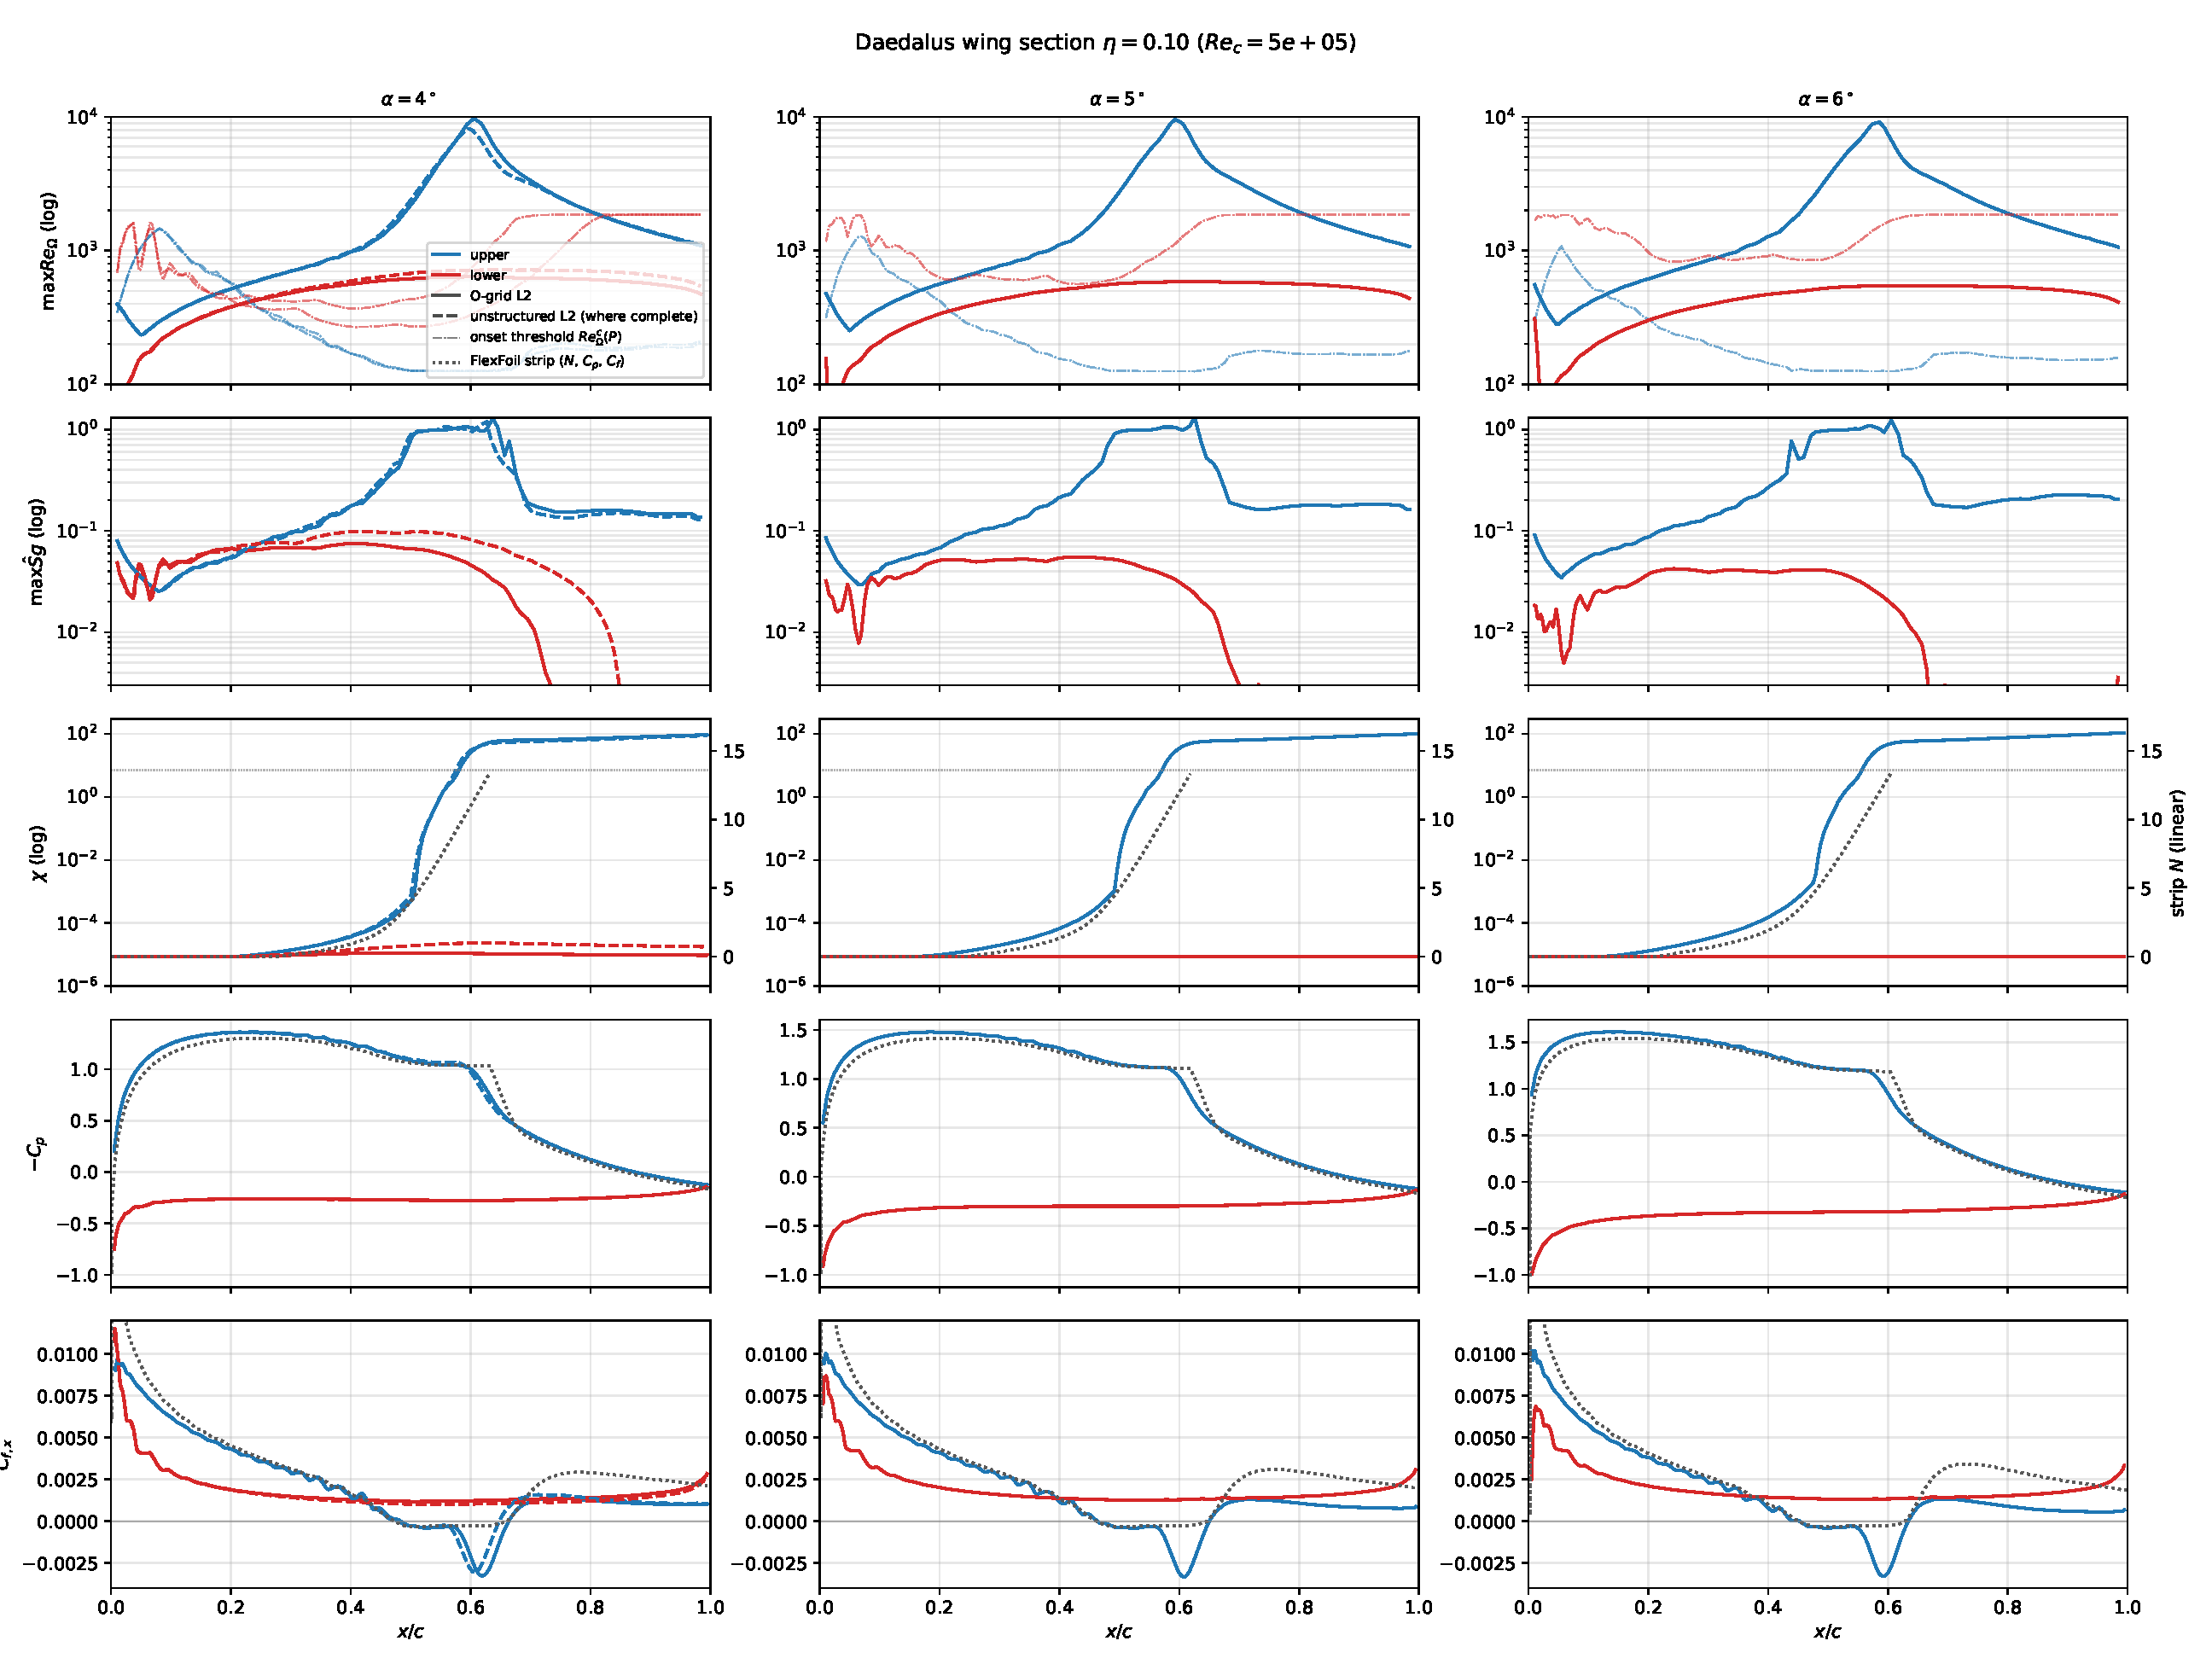
\includegraphics[width=0.99\textwidth]{daedalus_section_eta10.pdf}
  \caption{Daedalus wing section cut at $\eta=0.10$, $Re_c=5.0\times10^5$:
  sectional diagnostics on the finest grids (structured L2 solid;
  unstructured L2 dashed where its field output is available) against
  the AVL-trimmed FlexFoil/XFOIL strip (dotted) at $\alpha=4^\circ$,
  $5^\circ$, $6^\circ$ (columns).}
  \label{fig:daesec10}
\end{figure}

\begin{figure}[p]
  \centering
  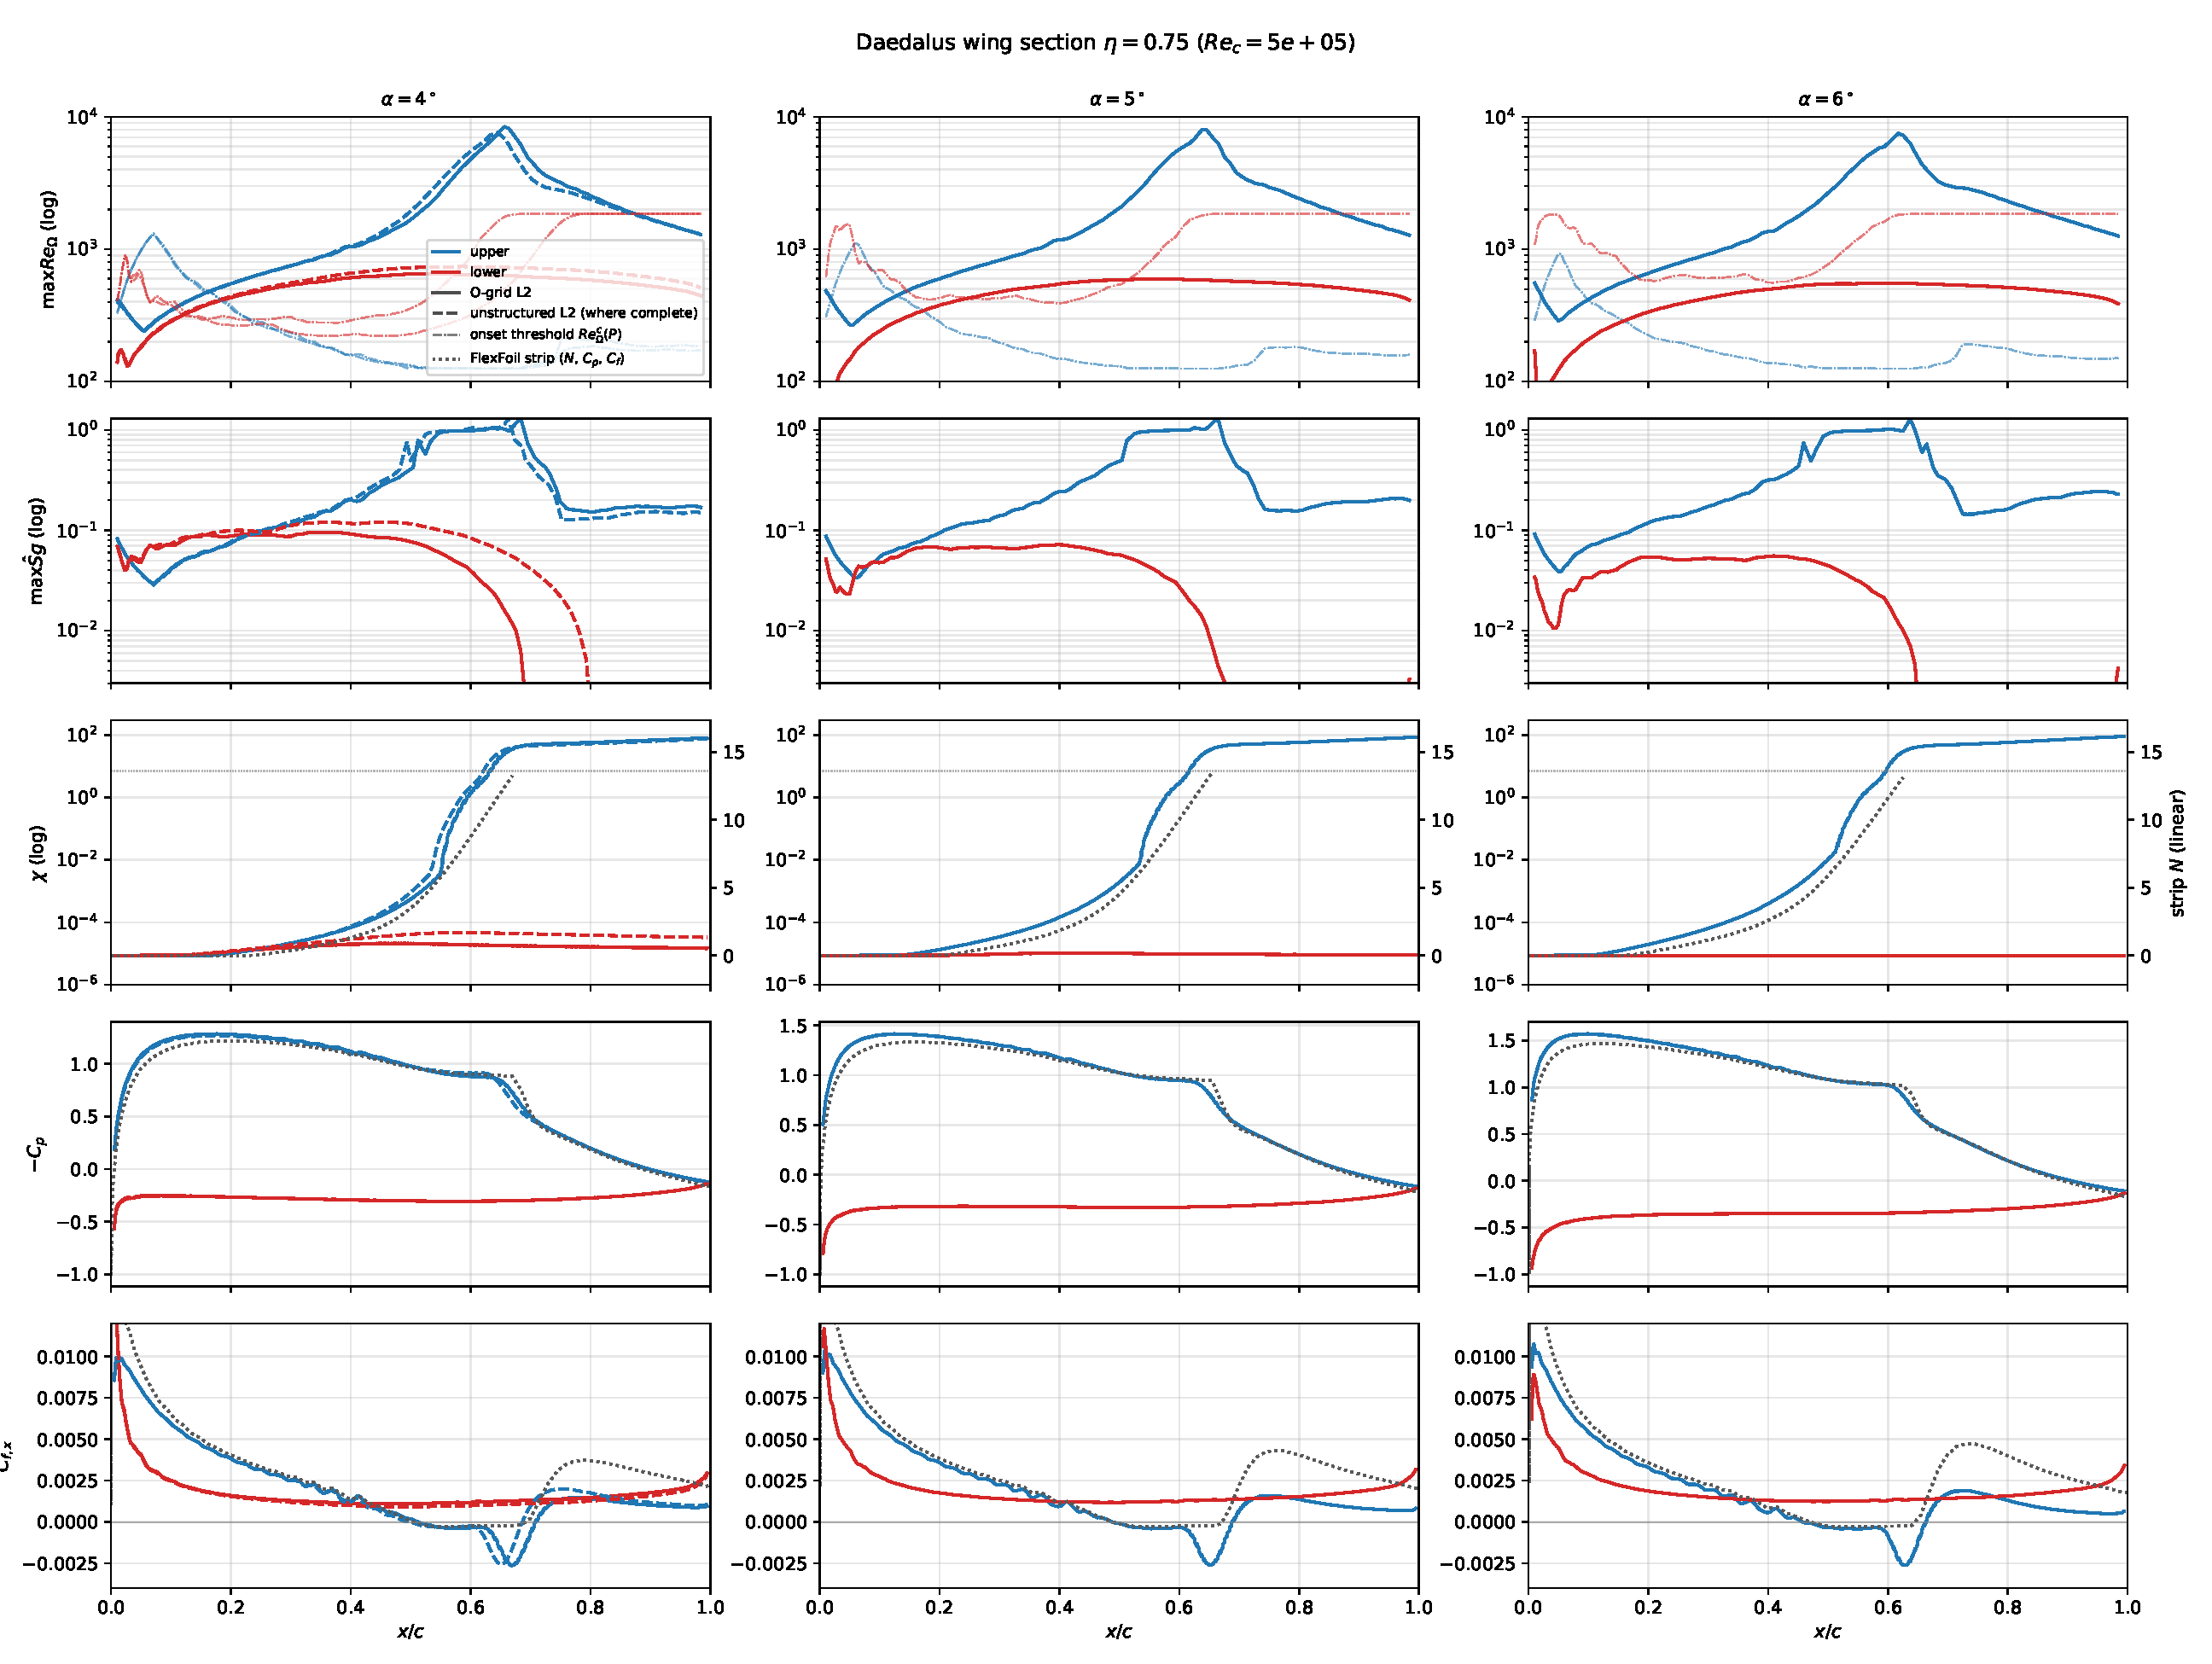
\includegraphics[width=0.99\textwidth]{daedalus_section_eta75.pdf}
  \caption{As Fig.~\ref{fig:daesec10}, at $\eta=0.75$.}
  \label{fig:daesec75}
\end{figure}

\begin{figure}[p]
  \centering
  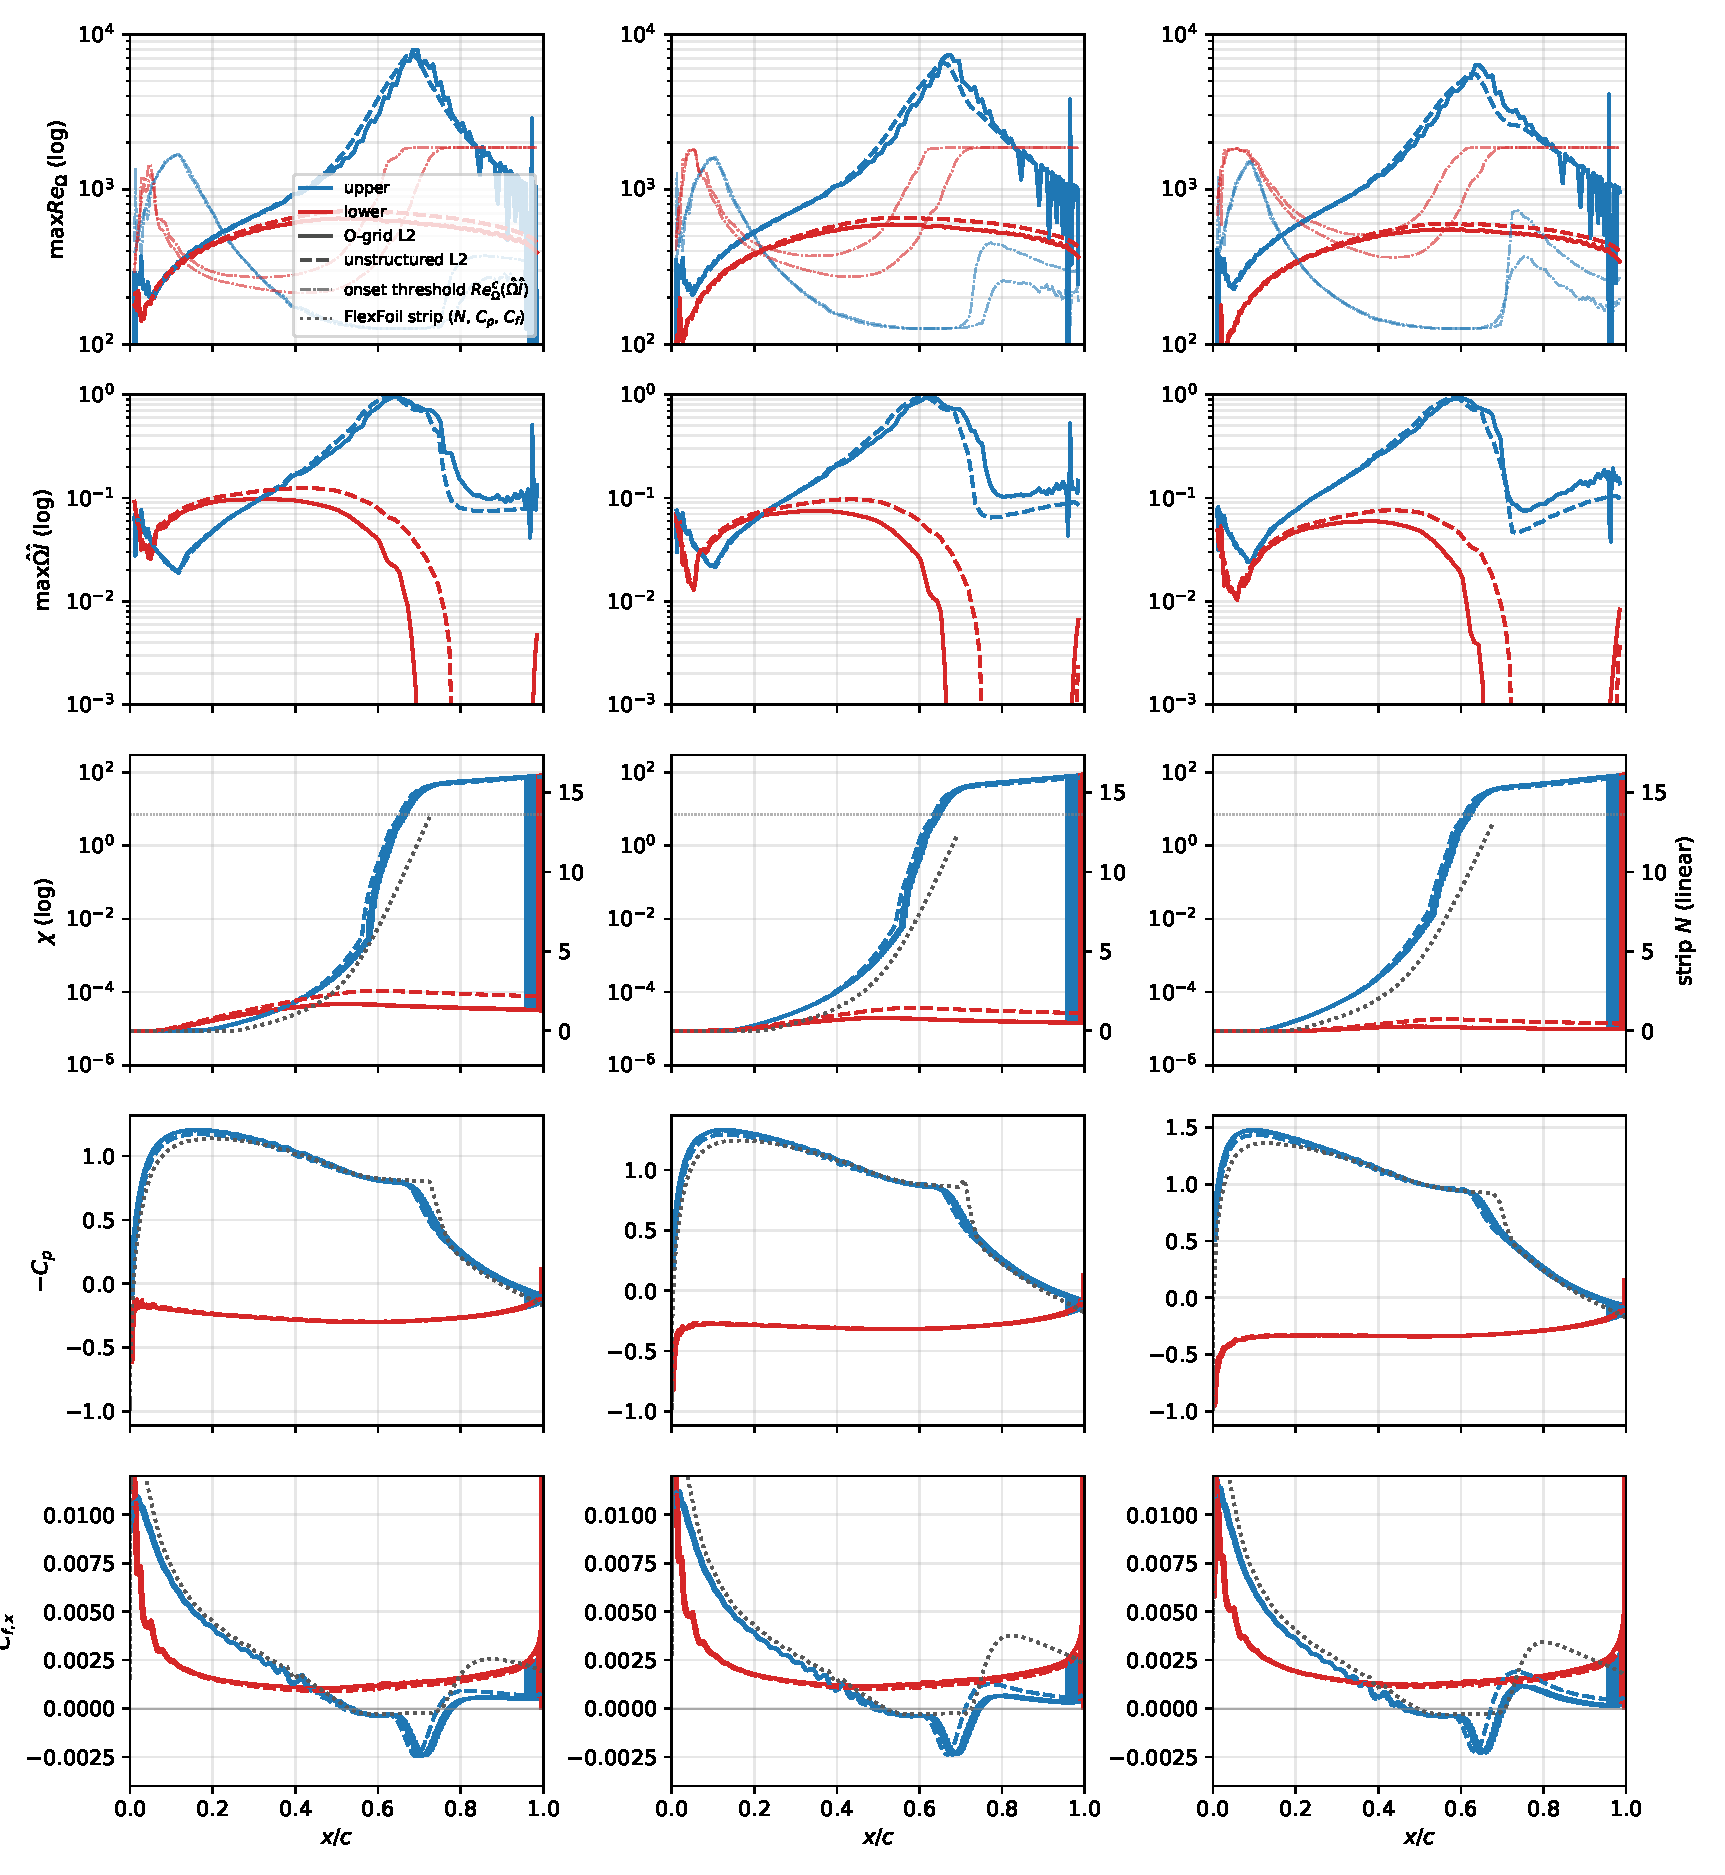
\includegraphics[width=0.99\textwidth]{daedalus_section_eta92.pdf}
  \caption{As Fig.~\ref{fig:daesec10}, at $\eta=0.92$---inside the
  taper, chord $0.728\,$m and $Re_c=4.0\times10^5$.}
  \label{fig:daesec92}
\end{figure}

\clearpage
\renewcommand{\thefigure}{E\arabic{figure}}
\renewcommand{\thetable}{E\arabic{table}}
\renewcommand{\theequation}{E\arabic{equation}}
\setcounter{figure}{0}\setcounter{table}{0}\setcounter{equation}{0}
\section*{Appendix E: the assembled one-equation model}\label{sec:assembled}

For reference, the complete model in one place. The working variable
$\tilde\nu$ obeys the single transport equation
\begin{equation}
  \frac{D\tilde\nu}{Dt} = P - D
  + \frac{1}{\sigma}\nabla\!\cdot\!\big[(c_{\nu,\mathrm{ai}}\,\nu+\tilde\nu)\,\nabla\tilde\nu\big]
  + \frac{c_{b2}}{\sigma}\,|\nabla\tilde\nu|^2,
  \label{eq:aisa}
\end{equation}
identical in form to Spalart--Allmaras~\cite{spalart_allmaras_1992} except in
four places---the blended production $P$ (its amplification branch built on
$\hat\Omega \hat I$), the tied destruction $D$, the
factor $c_{\nu,\mathrm{ai}}$ on the molecular diffusion, and the
lifted-layer bypass weight $b$ in the eddy-viscosity assembly;
$\sigma_P\!\equiv\!1$ (and with it $\sigma_D\!=\!1$),
$c_{\nu,\mathrm{ai}}\!=\!1$, and $b\!\equiv\!0$ recover baseline
SA exactly.

\paragraph{Terms.} The production and destruction are
\begin{equation}
  P = \max\!\big[\,(1-\sigma_P)\,a\,S\,\omega\,\tilde\nu,\;\;\sigma_P\,P_\mathrm{SA}\,\big],
  \qquad
  D = \sigma_D\,D_\mathrm{SA},
  \label{eq:aisa_pd}
\end{equation}
with the handover weights and the amplification rate restated below
(from Eqs.~\eqref{eq:indicators}--\eqref{eq:blend} and
\eqref{eq:sigmadtie}). The baseline SA
production, destruction, and closure functions, carried over unchanged, are
\begin{gather}
  P_\mathrm{SA} = c_{b1}\tilde S\,\tilde\nu, \qquad
  D_\mathrm{SA} = c_{w1}f_w\!\left(\frac{\tilde\nu}{d}\right)^{\!2}, \qquad
  \tilde S = \omega + \frac{\tilde\nu}{\kappa^2 d^2}\,f_{v2}, \qquad
  f_{v2} = 1 - \frac{\chi}{1+\chi f_{v1}}, \notag\\[3pt]
  f_{v1} = \frac{\chi^3}{\chi^3+c_{v1}^3}, \qquad
  f_w = g\!\left(\frac{1+c_{w3}^6}{g^6+c_{w3}^6}\right)^{\!1/6}, \qquad
  g = r + c_{w2}(r^6-r), \qquad
  r = \min\!\left(\frac{\tilde\nu}{\tilde S\,\kappa^2 d^2},\,10\right),
  \label{eq:sa_closure}
\end{gather}
with $\omega$ the vorticity magnitude, $\chi\!=\!\tilde\nu/\nu$, $d$ the wall
distance, and eddy viscosity
$\mu_t\!=\!\rho\tilde\nu\,[(1-b)f_{v1}+b]$ with the
lifted-layer bypass weight $b=s(\chi)G(q)$ of
Eqs.~\eqref{eq:fv1q}--\eqref{eq:fv1bypass}, where
$s=\mathrm{clip}(\chi-1,0,1)$, $G=\mathrm{clip}((q-2)/2,0,1)$, and
$U^+(y^+)$ in Eq.~\eqref{eq:fv1q} is Reichardt's law of the
wall~\cite{reichardt_1951},
$U^+=\tfrac1\kappa\ln(1+\kappa y^+)+7.8\,(1-e^{-y^+/11}-\tfrac{y^+}{11}e^{-y^+/3})$
(the wall-function
auxiliary $g$ is Spalart's, with its literature symbol restored now that the
coordinate rename freed it
below). We retain the
non-negative $\tilde S$ modification and the negative-$\tilde\nu$ safeguards
of Ref.~\cite{allmaras_2012}. The handover weights are
\begin{gather*}
  \sigma_P = \sigma_t(\chi;\tau), \qquad
  \sigma_t(\chi;\tau) = \max\!\left[\,1-e^{-(\chi-1)/\tau},\;0\right], \qquad
  \sigma_D = 1-\frac{c_{b1}}{\kappa^2c_{w1}}\,(1-\sigma_P),
\end{gather*}
and the amplification rate is built from four local vector-calculus
objects and their invariant pairings: the velocity $\mathbf u$,
measured relative to the nearest wall point (which makes the
indicators Galilean invariant; the absolute velocity for the
static-wall cases of this paper), the vorticity $\boldsymbol\omega$,
the wall-distance vector $\mathbf d=d\,\nabla d$ (so
$|\nabla d|\!=\!1$ and $\langle\mathbf d,\mathbf d\rangle\!=\!d^2$),
and the curvature vector
$\boldsymbol\ell=\tfrac12\langle\mathbf d,\mathbf d\rangle\,\nabla^2\mathbf u$,
with the divergence-free identity
$\nabla^2\mathbf u=-\nabla\times\boldsymbol\omega$ supplying the
second derivative. The indicator triple is their Gram form,
\begin{equation}
  (X,\,Y,\,Z) \;=\;
  \Big(\,\langle\mathbf u,\mathbf u\rangle,\;
  \sqrt{\langle\mathbf u,\mathbf u\rangle\,
        \langle\mathbf d,\mathbf d\rangle\,
        \langle\boldsymbol\omega,\boldsymbol\omega\rangle},\;
  \langle\boldsymbol\ell,\mathbf u\rangle\,\Big),
  \label{eq:gram}
\end{equation}
in which every entry is an invariant pairing, no unit vector appears,
no division by a vanishing magnitude can occur, and the only radical
sits over a non-negative product. From the triple,
\begin{gather*}
  \hat\Omega = \frac{Y}{\sqrt{X^2+Y^2}}, \qquad
  \hat I = \frac{Y-X-Z}{\sqrt{X^2+Y^2+Z^2}}, \qquad
  Re_\Omega = \frac{d^2\,|\boldsymbol\omega|}{\nu};
\end{gather*}
both $\hat\Omega$ and $\hat I$ are homogeneous of degree zero in the triple, so
any common positive factor drops out, and the solver's equivalent
ratio realization
$\big(|\mathbf u|,\,d|\boldsymbol\omega|,\,
\tfrac12 d^2(\nabla^2\mathbf u)\!\cdot\!\hat{\mathbf u}\big)$---the
arithmetic that produced every number in this paper---coincides with
Eq.~\eqref{eq:gram} wherever $\mathbf u\neq0$.

On a parallel layer
$\nabla^2\mathbf{u}=-\nabla\times\boldsymbol\omega=u''\,\hat{\mathbf{t}}$,
so the curvature projection reads $\operatorname{sign}(u)\,u''$---the
wall-normal derivative of the vorticity magnitude,
$\hat{\mathbf n}\!\cdot\!\nabla\omega$, in that limit---and the ratio
triple reduces to $(|u|,\,d|u'|,\,\tfrac12 d^2 u''\operatorname{sign}(u))$.
How these magnitude-based components realize the signed algebra of
Sec.~\ref{sec:model} (whose indicators, Eq.~\eqref{eq:indicators}, are
signed profile derivatives) is worth stating precisely: the
implemented parallel-layer triple is
$\big(\operatorname{sign}(u)\,u,\;\operatorname{sign}(u')\,d\,u',\;
\operatorname{sign}(u)\,\tfrac12 d^2u''\big)$. Wherever the velocity
and the shear share a sign---every attached profile, and all of a
reversed profile except the layer between its backflow extremum and
its velocity zero---the three components carry one common sign, so the
triple is a legitimate projective representative of the signed state
of Eq.~\eqref{eq:indicators}, and every even product, $\hat\Omega \hat I$
included, coincides with the theory \emph{exactly}: the magnitudes
realize the antipodal identification rather than break it (a globally
mirrored layer lands on the identified antipode), which is why the
calibration instruments of
Secs.~\ref{sec:calib_rate}--\ref{sec:calib_onset}, marched on attached
profiles, transfer to the solver unchanged. In the remaining
mixed-sign layer the implemented direction deviates from the signed
class in a single component's sign, and the deviation switches on and
off continuously: at the backflow extremum the affected component $Y$
itself vanishes, and at the velocity zero the state reaches the
$X\!=\!0$ meridian, where $\hat\Omega$ remains smooth and the curvature
projection changes sign with amplitude $\tfrac12 d^2|u''|$---small,
because the velocity zero of a free-shear-like reversed profile lies
close to its inflection point (for the antisymmetric layer the two
coincide and the amplitude is zero). The same four vectors admit two
other independent pairings, recorded here for completeness: the signed
pairing $\langle\boldsymbol\omega\times\mathbf d,\mathbf u\rangle$,
whose Cauchy--Schwarz \emph{envelope} is exactly Eq.~\eqref{eq:gram}'s
middle entry in two-dimensional flow, and its lower bound in three (by
the Lagrange identity
$|\boldsymbol\omega\times\mathbf d|^2=
\langle\mathbf d,\mathbf d\rangle\langle\boldsymbol\omega,\boldsymbol\omega\rangle-
\langle\boldsymbol\omega,\mathbf d\rangle^2$)---realizations built on
the signed pairing itself were implemented and rejected, as they
rectify vorticity-direction noise in weak shear---and the odd
(pseudoscalar) pairing
$\langle\nabla d,\mathbf u\times(\boldsymbol\omega\times\mathbf d)\rangle$,
which vanishes identically in two-dimensional flow, measures
crossflow, and is taken up in the outlook.

The rate $a$ (as in
Eq.~\eqref{eq:rate}) and its onset gate $S$ (as in Eq.~\eqref{eq:onset}) are
\begin{gather*}
  a = a_{\max}\,\operatorname{clip}\langle \hat\Omega \hat I\rangle_0^1, \qquad
  S = S\!\big(Re_\Omega/Re_\Omega^{\mathrm c}(\hat\Omega \hat I)\big), \qquad
  S(\zeta) = \tfrac12\big[1+\tanh\!\big((\zeta-1)/w\big)\big], \\[3pt]
  Re_\Omega^{\mathrm c}(\hat\Omega \hat I) = k\,\operatorname{softmin}_2\!\big(C,\;
      A + B\,\langle \hat\Omega \hat I\rangle_+^{-2}\big),
  \qquad \operatorname{softmin}_2(x_1,x_2) = \frac{x_1 x_2}{\sqrt{x_1^2+x_2^2}},
\end{gather*}
with $\langle x\rangle_+ = \max(x,0)$.

\paragraph{Constants.} The baseline SA constants are unchanged:
\begin{equation*}
  c_{b1}=0.1355,\quad \sigma=\tfrac{2}{3},\quad c_{b2}=0.622,\quad
  \kappa=0.41,\quad c_{w1}=\frac{c_{b1}}{\kappa^2}+\frac{1+c_{b2}}{\sigma},\quad
  c_{w2}=0.3,\quad c_{w3}=2,\quad c_{v1}=7.1 .
\end{equation*}
The SA-AI constants are
\begin{equation*}
  a_{\max}=0.19, \qquad
  (C,\,A,\,B;\;k)=(2600,\;175,\;2;\;0.712), \qquad
  w=0.35, \qquad
  \tau=4, \qquad
  c_{\nu,\mathrm{ai}}=\tfrac{1}{6},
\end{equation*}
with the freestream seed set by Mack's receptivity map,
$N_\mathrm{crit}(Tu)=-8.43-2.4\ln Tu_\mathrm{frac}$,
$\chi_\infty=c_{v1}e^{-N_\mathrm{crit}}$ (Eq.~\eqref{eq:tumap}).

\clearpage
\renewcommand{\thetable}{F\arabic{table}}
\setcounter{table}{0}
\section*{Appendix F: tabulated data for the one-dimensional comparison
figures}

Tables~\ref{tab:data_flatplate}--\ref{tab:data_eppresweep} tabulate the
computed values plotted in the paper's one-dimensional comparison
figures---forces, transition locations, and bubble stations---so exact
numbers need not be read off the plots. Conventions are those of the
corresponding figures: forces are medians over the final $20\%$ of the
pseudo-step history, transition locations are the near-wall $\chi\!=\!1$
front stations, and bubble stations are the signed-$C_f$ zero
crossings. The Daedalus totals are already tabulated in
Table~\ref{tab:daetotals}.

\begin{table}[tp]
  \centering\small
  \caption{Flat-plate transition-onset $Re_\theta$ (integrated from the computed profiles) at the $\chi\!=\!1$ and $\chi\!=\!c_{v1}$ crossings, Flow360 and the OpenFOAM replication (OF), against the Abu-Ghannam \& Shaw correlation (Fig.~\ref{fig:flatplate_batch}).}
  \label{tab:data_flatplate}
  \begin{tabular}{cccccc}
    \toprule
    $Tu$ [\%] & AGS $Re_\theta$ & $\chi\!=\!1$ & $\chi\!=\!c_{v1}$ & OF $\chi\!=\!1$ & OF $\chi\!=\!c_{v1}$ \\
    \midrule
    0.04 & 1126 & 1149 & 1203 & 1098 & 1154 \\
    0.08 & 1088 & 1002 & 1069 & 949 & 1004 \\
    0.16 & 1017 & 845 & 934 & 798 & 887 \\
    0.3 & 905 & 700 & 815 & 656 & 739 \\
    0.6 & 713 & 524 & 685 & 487 & 589 \\
    \bottomrule
  \end{tabular}
\end{table}

\begin{table}[tp]
  \centering\small
  \caption{NLF(1)-0416, $Re\!=\!4\!\times\!10^6$: computed forces and transition locations behind Figs.~\ref{fig:nlfaft}, \ref{fig:nlfpolar}, and~\ref{fig:nlfnegalpha}.}
  \label{tab:data_nlf}
  \begin{tabular}{ll cccc cccc}
    \toprule
    $\alpha$ & grid & \multicolumn{4}{c}{structured O-grid} & \multicolumn{4}{c}{unstructured cavity} \\ & & $C_L$ & $C_D$ & $x_\mathrm{tr}^\mathrm{up}$ & $x_\mathrm{tr}^\mathrm{lo}$ & $C_L$ & $C_D$ & $x_\mathrm{tr}^\mathrm{up}$ & $x_\mathrm{tr}^\mathrm{lo}$ \\
    \midrule
    $-8$ & L0 & -0.4426 & 0.01830 & 0.195 & 0.011 & -0.4689 & 0.01869 & 0.140 & 0.012 \\
    $-8$ & L1 & -0.4656 & 0.01093 & 0.538 & 0.006 & -0.4397 & 0.01150 & 0.571 & 0.011 \\
    $-8$ & L2 & -0.4646 & 0.00962 & 0.559 & 0.004 & -0.4426 & 0.00964 & 0.561 & 0.010 \\
    $-4$ & L0 & 0.0469 & 0.01078 & 0.435 & 0.100 & 0.0197 & 0.01025 & 0.476 & 0.083 \\
    $-4$ & L1 & 0.0142 & 0.00790 & 0.435 & 0.102 & 0.0357 & 0.00832 & 0.452 & 0.126 \\
    $-4$ & L2 & 0.0208 & 0.00718 & 0.447 & 0.109 & 0.0363 & 0.00739 & 0.453 & 0.122 \\
    $0$ & L0 & 0.5458 & 0.00803 & 0.400 & 0.590 & 0.4896 & 0.00808 & 0.355 & 0.592 \\
    $0$ & L1 & 0.5048 & 0.00607 & 0.395 & 0.553 & 0.5209 & 0.00660 & 0.392 & 0.579 \\
    $0$ & L2 & 0.5139 & 0.00564 & 0.387 & 0.566 & 0.5219 & 0.00606 & 0.391 & 0.569 \\
    $4$ & L0 & 1.0001 & 0.01090 & 0.250 & 0.645 & 0.9513 & 0.01062 & 0.330 & 0.621 \\
    $4$ & L1 & 0.9678 & 0.00800 & 0.238 & 0.610 & 0.9839 & 0.00805 & 0.269 & 0.614 \\
    $4$ & L2 & 0.9805 & 0.00730 & 0.255 & 0.610 & 0.9848 & 0.00772 & 0.260 & 0.621 \\
    $9$ & L0 & 1.4483 & 0.02252 & 0.015 & 0.385 & 1.4251 & 0.02345 & 0.105 & 0.641 \\
    $9$ & L1 & 1.4886 & 0.01436 & 0.065 & 0.625 & 1.5112 & 0.01353 & 0.085 & 0.635 \\
    $9$ & L2 & 1.5146 & 0.01245 & 0.073 & 0.628 & 1.5139 & 0.01286 & 0.078 & 0.638 \\
    $15$ & L0 & 1.5172 & 0.07109 & 0.010 & 0.440 & 1.3976 & 0.11602 & 0.005 & 0.623 \\
    $15$ & L1 & 1.9317 & 0.03159 & 0.004 & 0.650 & 1.9232 & 0.03454 & 0.001 & 0.659 \\
    $15$ & L2 & 2.0057 & 0.02628 & 0.005 & 0.659 & 1.9924 & 0.02772 & 0.000 & 0.662 \\
    \bottomrule
  \end{tabular}
\end{table}

\begin{table}[tp]
  \centering\small
  \caption{Eppler 387, $Re\!=\!2\!\times\!10^5$: computed forces behind the polar of Fig.~\ref{fig:epppolar} (the $-2^\circ$--$8.5^\circ$ extension incidences exist on the finest pair only).}
  \label{tab:data_epppolar}
  \begin{tabular}{ll cc cc}
    \toprule
    $\alpha$ & grid & \multicolumn{2}{c}{structured O-grid} & \multicolumn{2}{c}{unstructured cavity} \\ & & $C_L$ & $C_D$ & $C_L$ & $C_D$ \\
    \midrule
    $-2$ & L2 & 0.1750 & 0.01088 & 0.1791 & 0.01080 \\
    $0$ & L0 & 0.3859 & 0.01292 & 0.3847 & 0.01196 \\
    $0$ & L1 & 0.3843 & 0.01080 & 0.3969 & 0.01026 \\
    $0$ & L2 & 0.3844 & 0.01010 & 0.3894 & 0.01030 \\
    $1$ & L2 & 0.4960 & 0.01079 & 0.5013 & 0.01092 \\
    $2$ & L0 & 0.6079 & 0.01381 & 0.6061 & 0.01246 \\
    $2$ & L1 & 0.6048 & 0.01196 & 0.6207 & 0.01152 \\
    $2$ & L2 & 0.6059 & 0.01154 & 0.6124 & 0.01167 \\
    $3$ & L2 & 0.7146 & 0.01249 & 0.7215 & 0.01247 \\
    $4$ & L2 & 0.8216 & 0.01354 & 0.8304 & 0.01338 \\
    $5$ & L0 & 0.9083 & 0.02007 & 0.9253 & 0.01596 \\
    $5$ & L1 & 0.9218 & 0.01575 & 0.9465 & 0.01444 \\
    $5$ & L2 & 0.9274 & 0.01451 & 0.9375 & 0.01428 \\
    $6$ & L2 & 1.0346 & 0.01453 & 1.0459 & 0.01437 \\
    $7$ & L0 & 1.0639 & 0.02728 & 1.1241 & 0.02038 \\
    $7$ & L1 & 1.1262 & 0.01686 & 1.1593 & 0.01557 \\
    $7$ & L2 & 1.1415 & 0.01431 & 1.1535 & 0.01419 \\
    $8.5$ & L2 & 1.2197 & 0.02361 & 1.2426 & 0.02258 \\
    \bottomrule
  \end{tabular}
\end{table}

\begin{table}[tp]
  \centering\small
  \caption{Eppler 387, $Re\!=\!2\!\times\!10^5$: computed upper-surface laminar-separation and turbulent-reattachment stations behind Fig.~\ref{fig:eppbubble} (signed-$C_f$ zero crossings; missing entries transition ahead of separation and have no bubble).}
  \label{tab:data_eppbubble}
  \begin{tabular}{ll cc cc}
    \toprule
    $\alpha$ & grid & \multicolumn{2}{c}{structured O-grid} & \multicolumn{2}{c}{unstructured cavity} \\ & & $x_{LS}/c$ & $x_R/c$ & $x_{LS}/c$ & $x_R/c$ \\
    \midrule
    $-2$ & L2 & 0.573 & 0.822 & 0.567 & 0.815 \\
    $0$ & L0 & 0.549 & 0.720 & 0.540 & 0.711 \\
    $0$ & L1 & 0.526 & 0.771 & 0.526 & 0.737 \\
    $0$ & L2 & 0.523 & 0.761 & 0.520 & 0.757 \\
    $1$ & L2 & 0.500 & 0.740 & 0.499 & 0.733 \\
    $2$ & L0 & 0.490 & 0.656 & 0.512 & 0.649 \\
    $2$ & L1 & 0.479 & 0.713 & 0.483 & 0.682 \\
    $2$ & L2 & 0.477 & 0.714 & 0.478 & 0.706 \\
    $3$ & L2 & 0.454 & 0.691 & 0.454 & 0.679 \\
    $4$ & L2 & 0.426 & 0.667 & 0.430 & 0.657 \\
    $5$ & L0 & 0.393 & 0.568 & 0.429 & 0.558 \\
    $5$ & L1 & 0.394 & 0.624 & 0.415 & 0.600 \\
    $5$ & L2 & 0.402 & 0.634 & 0.404 & 0.623 \\
    $6$ & L2 & 0.388 & 0.565 & 0.391 & 0.560 \\
    $7$ & L0 & 0.250 & 0.343 & 0.351 & 0.458 \\
    $7$ & L1 & -- & -- & -- & -- \\
    $7$ & L2 & 0.388 & 0.407 & -- & -- \\
    $8.5$ & L2 & 0.031 & 0.039 & 0.019 & 0.049 \\
    \bottomrule
  \end{tabular}
\end{table}

\begin{table}[tp]
  \centering\small
  \caption{Eppler 387 $\alpha\!=\!5^\circ$ Reynolds sweep: computed forces and upper-surface stations behind Fig.~\ref{fig:eppresweepforces} ($x_R$ pinned near $1$ means no closure ahead of the trailing edge; $c_m$ and the $e^9$/experiment columns are in Table~\ref{tab:eppresweep}). The $2\times10^5$ rows are the figure script\'s own re-extraction of the benchmark histories and agree with Table~\ref{tab:data_epppolar}\'s campaign-record values to within one unit in the last digit (tail-window rounding).}
  \label{tab:data_eppresweep}
  \begin{tabular}{ll cccc cccc}
    \toprule
    $Re$ & grid & \multicolumn{4}{c}{structured O-grid} & \multicolumn{4}{c}{unstructured cavity} \\ & & $c_l$ & $c_d$ & $x_\mathrm{sep}$ & $x_R$ & $c_l$ & $c_d$ & $x_\mathrm{sep}$ & $x_R$ \\
    \midrule
    $60$k & L0 & 0.6648 & 0.04879 & 0.317 & 0.994 & 0.8377 & 0.03560 & 0.374 & 0.996 \\
    $60$k & L1 & 0.6606 & 0.05064 & 0.329 & 0.996 & 0.7777 & 0.04373 & 0.344 & 0.998 \\
    $60$k & L2 & 0.6362 & 0.05330 & 0.319 & 0.997 & 0.7123 & 0.05065 & 0.325 & 0.999 \\
    $100$k & L0 & 0.8245 & 0.03320 & 0.360 & 0.994 & 0.8929 & 0.02349 & 0.401 & 0.977 \\
    $100$k & L1 & 0.8401 & 0.03336 & 0.347 & 0.997 & 0.9011 & 0.02475 & 0.382 & 0.951 \\
    $100$k & L2 & 0.7952 & 0.04103 & 0.328 & 0.999 & 0.8773 & 0.03071 & 0.349 & 0.992 \\
    $200$k & L0 & 0.9084 & 0.02007 & 0.393 & 0.568 & 0.9253 & 0.01596 & 0.429 & 0.558 \\
    $200$k & L1 & 0.9220 & 0.01577 & 0.394 & 0.624 & 0.9465 & 0.01444 & 0.415 & 0.600 \\
    $200$k & L2 & 0.9275 & 0.01451 & 0.402 & 0.634 & 0.9377 & 0.01427 & 0.404 & 0.623 \\
    $300$k & L0 & 0.9233 & 0.01718 & 0.391 & 0.494 & 0.9364 & 0.01351 & 0.442 & 0.529 \\
    $300$k & L1 & 0.9352 & 0.01213 & 0.423 & 0.545 & 0.9600 & 0.01155 & 0.435 & 0.548 \\
    $300$k & L2 & 0.9410 & 0.01073 & 0.435 & 0.551 & 0.9499 & 0.01083 & 0.437 & 0.549 \\
    $460$k & L0 & 0.9341 & 0.01535 & -- & -- & 0.9453 & 0.01154 & -- & -- \\
    $460$k & L1 & 0.9444 & 0.00998 & -- & -- & 0.9704 & 0.00959 & 0.462 & 0.490 \\
    $460$k & L2 & 0.9499 & 0.00870 & 0.467 & 0.482 & 0.9589 & 0.00886 & 0.471 & 0.482 \\
    \bottomrule
  \end{tabular}
\end{table}


\end{document}
